\PassOptionsToPackage{outputdir=_build}{minted}
\PassOptionsToPackage{dvipsnames,usenames}{color}
% Load the kaobook class
\documentclass[
  french,english,
  fontsize=10pt, % Base font size
  twoside=true, % Use different layouts for even and odd pages (in particular, if twoside=true, the margin column will be always on the outside)
  %open=any, % If twoside=true, uncomment this to force new chapters to start on any page, not only on right (odd) pages
  secnumdepth=2, % How deep to number headings. Defaults to 1 (sections)
  numbers=enddot,
]{kaobook/kaobook}

% Choose the language
\usepackage{babel} % Load characters and hyphenation
\usepackage[english=british]{csquotes}	% English quotes

% Load packages for testing
\usepackage{blindtext}
\usepackage{comment}
%\usepackage{showframe} % Uncomment to show boxes around the text area, margin, header and footer
%\usepackage{showlabels} % Uncomment to output the content of \label commands to the document where they are used

% Load the bibliography package
\usepackage[style=alphabetic,maxbibnames=99,useprefix=true]{kaobook/kaobiblio}
\DefineBibliographyExtras{french}{\restorecommand\mkbibnamefamily} %To have consistent citations between French and English text
\addbibresource{biblio.bib} % Bibliography file

%Load my own style
\usepackage{styles/layout}

% Load mathematical packages for theorems and related environments
\usepackage[boxed]{kaobook/kaotheorems}

% Load the package for hyperreferences
\usepackage{kaobook/kaorefs}

% Macros are after the knowledge package
%TC:ignore
% \knowledgestyle*{notion}{style={color=black!80!},intro style={color=black!80!,emphasize}}

\knowledgestyle{black}{color=black}
\knowledgestyle{no}{color=.}
\knowledgestyle{notion intro}{color=LightOrange,emphasize}
\knowledgedirective*{notion}{autoref,style=black,intro style=notion intro}

\knowledgedirective*{automatic in command}{autoref,style=no,intro style=no}

\knowledgestyle{ignore intro}{color=LightOrange,emphasize}
\knowledgedirective*{ignore}{intro style=ignore intro}

\knowledgedirective{title}{}

\knowledgedirective{system}{smallcaps}

% Systems

\knowledge{system}
  | Idris

\knowledge{system}
  | Coq

\knowledge{system}
  | Agda

\knowledge{system}
  | Lean

\knowledge{system}
  | Gallina@fr

\knowledge{system}
  | Gallina

\knowledge{system}
  | MetaCoq

\knowledge{system}
  | Matita

\knowledge{system}
  | GitHub

\knowledge{system}
  | Dependent Haskell

\knowledge{system}
  | Equations

% Mathematical Macros
\knowledge{automatic in command}
  | \uni{}

\knowledge{automatic in command}
  | \pair{}

\knowledge{automatic in command}
  | \lnil{}

\knowledge{automatic in command}
  | \vnil{}

\knowledge{automatic in command}
  | \?

\knowledge{automatic in command}
  | \err{}

\knowledge{automatic in command}
  | \cast{}

\knowledge{automatic in command}
  | \rai{}

% Pre-text

\knowledge{notion}
  | example

%Chapter 1

\knowledge{ignore}
  | type@fr
  | types@fr

\knowledge{notion}
  | type dépendant
  | types dépendants
  | théorie des types dépendants
  | dépendant@typ
  | dépendants@typ

\knowledge{notion}
  | assistant à la preuve
  | assistants à la preuve

\knowledge{notion}
  | correspondance de Curry-Howard
  | correspondance preuves-programmes

\knowledge{notion}
  | noyau

\knowledge{notion}
  | critère de De Bruijn

\knowledge{notion}
  | bidirectionnel
  | typage bidirectionnel

\knowledge{notion}
  | graduel
  | graduels
  | typage graduel
  | type graduel
  | types graduels

% Chapter 2

\knowledge{ignore}
  | type@en
  | types@en

\knowledge{notion}
  | dependent type
  | dependent types
  | dependent@typ
  | dependently

\knowledge{notion}
  | Curry-Howard correspondence

\knowledge{notion}
  | kernel

\knowledge{notion}
  | De Bruijn criterion

\knowledge{notion}
  | proof assistant
  | proof assistants

\knowledge{notion}
  | bidirectional
  | bidirectional typing

% Chapter 3

\knowledge{notion}
  | substitution

% Section 3.2

\knowledge{notion}
  | Calculus of Constructions

\knowledge{notion, text={CC\textsubscript{ω}}}
  | CCω

\knowledge{title, text={CC\textsubscript{ω}}}
  | CCω@tit

\knowledge{title}
  | Calculus of Constructions@tit

\knowledge{notion}
  | CIC

\knowledge{notion}
  | Calculus of Inductive Constructions

\knowledge{title}
  | CIC@tit

\knowledge{title}
  | Calculus of Inductive Constructions@tit

\knowledge{notion}
  | Polymorphic, Cumulative Calculus of Inductive Constructions

\knowledge{notion}
  | PCUIC

\knowledge{title}
  | PCUIC@tit

\knowledge{notion}
  | α-equality
  | α-equal 

\knowledge{notion}
  | Church-style

\knowledge{notion}
  | Curry-style

\knowledge{notion}
  | universe level
  | universe levels
  | level
  | levels

\knowledge{notion}
  | typical ambiguity


% Section 3.3 
\knowledge{notion}
  | conversion
  | convertible

\knowledge{notion}
  | typed conversion
  | Typed conversion
  | typed@conv

\knowledge{notion}
  | untyped conversion
  | Untyped conversion
  | untyped@conv

\knowledge{notion}
  | Pure Type Systems
  | Pure Type System
  | PTS

\knowledge{notion}
  | declarative conversion
  | Declarative conversion
  | declarative@conv
  | conversion@decl

\knowledge{notion}
  | algorithmic conversion
  | algorithmic@conv
  | Algorithmic@conv
  | conversion@algo

\knowledge{notion}
  | reduction
  | Reduction

\knowledge{notion}
  | top-level reduction
  | Top-level reduction
  | top-level reductions
  | top-level@red

\knowledge{notion}
  | one-step reduction
  | one-step@red
  | One-step reduction

\knowledge{notion}
  | weak-head reduction
  | weak-head@red
  | Weak-head reduction

\knowledge{notion}
  | full reduction
  | Full reduction
  | full@red

% Section 3.4
\knowledge{notion}
  | stability under renaming
  | Stability under renaming
  | stable under renaming

\knowledge{notion}
  | weakening
  | Weakening

\knowledge{notion}
  | stability under substitution
  | Stability under substitution
  | stable under substitution

\knowledge{notion}
  | conditional stability under renaming
  | Conditional stability under renaming


\knowledge{notion}
  | strengthening
  | Strengthening

\knowledge{notion}
  | uniqueness of types up to
  | uniqueness of types
  | Uniqueness of types
  | uniqueness@typ

\knowledge{notion}
  | validity
  | Validity

\knowledge{notion}
  | Subject reduction
  | subject reduction
  | preservation

\knowledge{notion}
  | injectivity of function types
  | Injectivity of function types
  | injectivity of type constructors

\knowledge{notion}
  | confluence
  | Confluence
  | confluent

\knowledge{notion}
  | normal form
  | normal forms
  | Normal

\knowledge{notion}
  | neutral form
  | neutral forms
  | neutral
  | neutrals
  | Neutral

\knowledge{notion}
  | canonical form
  | canonical forms

\knowledge{notion}
  | progress
  | Progress

\knowledge{notion}
  | safety
  | Safety
  | safe

\knowledge{notion}
  | accessible
  | Accessibility

\knowledge{notion}
  | Normalization
  | normalization
  | normalizing

\knowledge{notion}
  | logical consistency
  | logically consistent
  | Logical consistency
  | consistency@log
  | consistent@log

\knowledge{notion}
  | closed term
  | closed terms
  | closed
  | open
  | open term

\knowledge{notion}
  | canonicity
  | Canonicity

% Section 3.5 
\knowledge{notion}
  | inductive type
  | inductive types

\knowledge{notion}
  | boolean
  | booleans

\knowledge{notion}
  | constructor
  | constructors

\knowledge{notion}
  | recursor
  | recursors
  | induction principle

\knowledge{notion}
  | scrutinee
  | predicate
  | branches

\knowledge{notion}
  | fully applied

\knowledge{notion}
  | indexed@ind
  | indexed inductive type
  | indexed inductive types
  | index
  | indices

\knowledge{notion, text ={CIC\textsubscript{$-$}}}
  | CIC-

% Section 3.6
\knowledge{notion}
  | cumulativity
  | Cumulativity

\knowledge{notion}
  | α-pre-order

\knowledge{notion}
  | impredicativity

\knowledge{notion}
  | proof irrelevance

\knowledge{notion}
  | local definitions
  | local definition

\knowledge{notion}
  | environment
  | global environment

\knowledge{notion}
  | universe polymorphism
  | universe polymorphic

\knowledge{notion}
  | guard condition

\knowledge{notion}
  | record type
  | record types
  | record@type

\knowledge{notion}
  | projection
  | projections

\knowledge{notion}
  | co-inductive type
  | co-inductive types

% Bidirectional part

\knowledge{notion}
  | mode
  | modes
  | subject
  | subjects
  | inputs
  | input
  | outputs
  | output

\knowledge{notion}
  | undirected typing
  | undirected@typ

% Chapter 4

\knowledge{notion}
  | well-formed
  | well-typed

\knowledge{notion}
  | inference

\knowledge{notion}
  | checking

\knowledge{notion}
  | boundary

\knowledge{notion}
  | constrained inference

\knowledge{notion}
  | full

\knowledge{notion}
  | type-level enforcing

\knowledge{notion}
  | Correctness
  | correctness@bidir
  | correct@bidir
  | Correctness@bidir

\knowledge{notion}
  | Soundness
  | soundness@bidir
  | sound@bidir
  | Soundness@bidir

\knowledge{notion}
  | Completeness
  | completeness@bidir
  | Completeness@bidir
  | complete@bidir

% Chapter 5

\knowledge{notion}
  | principal type
  | principal types
  | principal@type

% Chapter 6

\knowledge{notion}
  | Generic conversion
  | generic conversion

\knowledge{notion}
  | Neutral comparison
  | neutral comparison

\knowledge{notion}
  | Generic cumulativity
  | generic cumulativity



% MetaCoq

% MetaCoq Tour

\knowledge{notion}
  | conversion problem

\knowledge{notion}
  | well-scoped
  | well-scoping

\knowledge{notion}
  | parallel reduction
  | Parallel reduction

\knowledge{notion}
  | diamond property

\knowledge{notion}
  | best parallel reduct

% Gradual CIC

\knowledge{notion}
  | gradual@typ
  | Gradual typing
  | gradual typing
  | gradual types

\knowledge{notion}
  | consistency@grad
  | consistent@grad

\knowledge{notion}
  | Fire Triangle of Graduality

\knowledge{notion}
  | Gradual Calculus of Inductive Constructions
  | GCIC

\knowledge{title}
  | GCIC@tit

% Chapter 9

\knowledge{notion,text={CIC+$\axiom$}}
  | CICax

\knowledge{ignore,text={CIC+$\rai$}}
  | CICrai

\knowledge{notion}
  | ExTT

\knowledge{notion}
  | unknown term
  | unknown terms
  | unknown type
  | unknown

\knowledge{notion}
  | gradual guarantee
  | gradual guarantees

\knowledge{notion}
  | ascription

\knowledge{notion}
  | simply-typed lambda calculus
  | simply-typed

\knowledge{notion}
  | STLC

\knowledge{title}
  | STLC@tit

\knowledge{notion}
  | GTLC

\knowledge{notion}
  | error
  | errors

\knowledge{notion}
  | call-by-name

\knowledge{notion}
  | cast
  | casts

\knowledge{notion}
  | conservative extension
  | Conservativity
  | conservativity
  | conservative

\knowledge{notion}
  | precision
  | precise

\knowledge{notion}
  | static gradual guarantee
  | Static Gradual Guarantee

\knowledge{notion}
  | SGG

\knowledge{notion}
  | dynamic gradual guarantee
  | Dynamic Gradual Guarantee

\knowledge{notion}
  | DGG

\knowledge{notion}
  | observational error-approximation
  | Observational error-approximation
  | observationally error-approximates

\knowledge{notion}
  | observationally equivalent
  | observational equivalence

\knowledge{notion}
  | embedding-projection pairs
  | ep-pairs
  | ep-pair
  | embedding-projection

\knowledge{notion}
  | equi-precise
  | equi-precision

\knowledge{notion}
  | graduality
  | Graduality

\knowledge{ignore}
  | consistent lifting

\knowledge{ignore}
  | higher-order unification

\knowledge{notion}
  | observational refinement
  | Observational refinement
  | observationally refines

\knowledge{notion}
  | GDTL

\knowledge{notion}
  | Approximate Normalization

\knowledge{notion, text={CIC\textsuperscript{$\uparrow$}}}
  | CICs

\knowledge{notion, text={GCIC\textsuperscript{$\mathcal{G}$}}}
  | GCICP

\knowledge{notion, text={GCIC\textsuperscript{$\uparrow$}}}
  | GCICs

\knowledge{notion, text={GCIC\textsuperscript{$\mathcal{N}$}}}  
  | GCICT

\knowledge{notion, text={CastCIC}}
  | CastCIC
  | CCIC

\knowledge{title, text={CastCIC}}
  | CastCIC@tit
  | CCIC@tit

\knowledge{notion, text={CastCIC\textsuperscript{$\mathcal{G}$}}}
  | CCICP

\knowledge{notion, text={CastCIC\textsuperscript{$\uparrow$}}}
  | CCICs

\knowledge{notion, text={CastCIC\textsuperscript{$\mathcal{N}$}}}  
  | CCICT

\knowledge{notion}
  | syntactic@pre
  | precision@syn
  | syntactic precision
  | Syntactic precision

\knowledge{notion}
  | structural@pre
  | precision@str
  | structural precision
  | Structural precision
  | Structural@pre
  | Structural
  | structural

\knowledge{notion}
  | propositional@pre
  | precision@prop
  | propositional precision
  | Propositional precision
  | propositional

% Chapter 10

\knowledge{notion}
 | head constructor
 | Head constructor
 | head constructors

\knowledge{notion}
  | germ

\knowledge{notion}
  | static
  | static term

\knowledge{notion}
  | catch-up lemmas

\knowledge{notion}
  | simulation

\knowledge{notion}
  | α-consistency
  | α-consistent

\knowledge{notion}
  | consistent conversion
  | Consistent conversion
  | consistently convertible

\knowledge{notion}
  | Definitional precision
  | definitional precision
  | definitional@pre
  | Definitional
  | definitional

\knowledge{notion}
  | erasability
  | erasure
  | Erasure
  | erasable

\knowledge{notion}
  | elaboration graduality
  | Elaboration Graduality

\knowledge{notion}
  | universe adequate
  | universe adequacy

% Chapter 11

\knowledge{notion}
  | discrete model

\knowledge{notion}
  | monotone model

\knowledge{notion}
  | syntactic model
  | Syntactic models

\knowledge{notion}
  | concretely forceable

\knowledge{notion, text = {GRIP}}
  | CCICPrec
  | GRIP

\knowledge{notion}
  | RETT

\knowledge{notion, text={\textsc{TTObs}}}
  | TTOBS

\knowledge{notion}
  | internal precision
  | Internal precision

\knowledge{notion}
  | self-precise
  | self-precision

%TC:endignore
\usepackage{styles/macros}
\usepackage{styles/alectryon-minted}

\includeonly{header,intro,formal-intro,formal-kernel,formal-statics.gen,formal-discussion,mem-model-intro,mem-model-cn,eng-intro,eng-usable,conclusion}
%\includeonly{formal-statics.gen}

\graphicspath{{./figures/}} % Paths where images are looked for

% the un-wrapped (-tex_wrap false) generated LaTeX file for CN
%TC:ignore
\input{cn_included.gen}
% the package that allows customized layout described in this document
\usepackage{ott/ottlayout}
% the automatically generated file (with our Makefile) to link the generated
% LaTeX with the ottlayout package
\input{cn_override.gen}
\input{cn_drulenames.gen}
% Put judgement comment on a new line, half-BLS below the judgement form (in a box)
\renewenvironment{cndefnblock}[3][]{ \framebox{\mbox{#2}} \\[0.5\baselineskip] #3 \\[0pt]}{}
% Hide bind specs, and put comment on a new line underneath judgements
\newcommand{\cnprodlineCommentNewline}[6]{& & $#1$ & $#2$ & $#3$ & $#5$ & \\ & & & \multicolumn{4}{p{\textwidth} }{#6} }
% Hide bind specs
\renewcommand{\cnprodline}[6]{& & $#1$ & $#2$ & $#3$ & $#5$ & #6}
% Hide bind specs
\renewcommand{\cnbindspecprodline}[6]{}
\ottstyledefaults{numberpremises=yes,premisenamelayout=topright,rulelayout=nobreaks}
% Initially I wanted to pass in a list of macro invocations as the first
% argument, but I could not make that work (couldn't figure out how to split
% \detokenized{#1} by comma, such that I could lookup the \detokenized{##1} to
% the renewed \cnusedrule in that split list).
% Then I tried numbers, and this also I could not make work with a flag of some
% sort set inside the \foreach loop (it would set the flag, and then reset it
% after exiting the loop). So now it just prints like this, and duplicate numbers
% are simpy a call-site error.
\newcommand{\FilterUsedRules}[2]{%
  \begingroup
  \def\allowedNs{#1}%
  \newcount\nthcall%
  \nthcall=0

  \NewCommandCopy{\origcnusedrule}{\cnusedrule}

  \renewcommand{\cnusedrule}[1]{%
    \advance\nthcall by 1% chktex 1
    \foreach\n in \allowedNs{%
      \ifnum\nthcall=\n%
        \origcnusedrule{##1}
      \fi%
    }
  }

  #2
  \endgroup
}
%TC:endignore

%\makeindex[columns=3, title=Alphabetical Index, intoc] % Make LaTeX produce the files required to compile the index

\begin{document}

%----------------------------------------------------------------------------------------
%	BOOK INFORMATION
%----------------------------------------------------------------------------------------

% \titlehead{Document Template}
\title[Working Title: Why did JT release the 20/20 experience in 2013?]{Working Title: Why did JT release the 20/20 experience in 2013?}
\subtitle{Doctoral Thesis}
\author[D. C. Makwana]{Dhruv C. Makwana}%
\date{\today \\[\baselineskip] 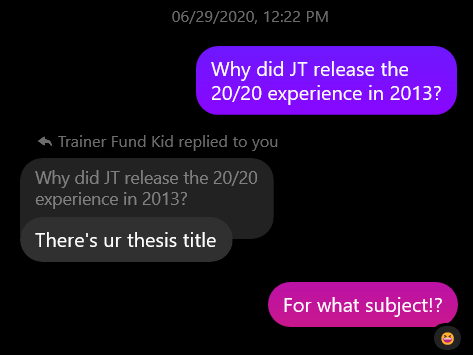
\includegraphics[width=.8\textwidth]{figures/working-title.png}
}
% \publishers{An Awesome Publisher}

%----------------------------------------------------------------------------------------

\frontmatter % Denotes the start of the pre-document content, uses roman numerals

%----------------------------------------------------------------------------------------
%	COPYRIGHT PAGE
%----------------------------------------------------------------------------------------

% \makeatletter
% \uppertitleback{\@titlehead} % Header
%
% \lowertitleback{%
% 	% \textbf{Disclaimer} \\
% 	% You can edit this page to suit your needs. For instance, here we have a no copyright statement, a colophon and some other information. This page is based on the corresponding page of Ken Arroyo Ohori's thesis, with minimal changes.
%
% 	% \medskip
%
% 	% \textbf{No copyright} \\
% 	% \cczero\ This book is released into the public domain using the CC0 code. To the extent possible under law, I waive all copyright and related or neighbouring rights to this work.
%
% 	% To view a copy of the CC0 code, visit: \\\url{http://creativecommons.org/publicdomain/zero/1.0/}
%
% 	% \medskip
%
% 	% \textbf{Colophon} \\
% 	% This document was typeset with the help of \href{https://sourceforge.net/projects/koma-script/}{\KOMAScript} and \href{https://www.latex-project.org/}{\LaTeX} using the \href{https://github.com/fmarotta/kaobook/}{kaobook} class.
%
% 	% \medskip
%
% 	% \textbf{Publisher} \\
% 	% First printed in May 2019 by \@publishers
% }
% \makeatother

%----------------------------------------------------------------------------------------
%	DEDICATION
%----------------------------------------------------------------------------------------

\dedication{\raggedleft\emph{To \_,\\
Something short and sweeet.}}

% \dedication{
% 	% The harmony of the world is made manifest in Form and Number, and the heart and soul and all the poetry of Natural Philosophy are embodied in the concept of mathematical beauty.\\
% 	% \flushright -- D'Arcy Wentworth Thompson
% }

%----------------------------------------------------------------------------------------
%	OUTPUT TITLE PAGE AND PREVIOUS
%----------------------------------------------------------------------------------------

% \includepdf[pages=1]{../MathSTICTemplate/main.pdf}

% Note that \maketitle outputs the pages before here
\maketitle

%----------------------------------------------------------------------------------------
%	PREFACE
%----------------------------------------------------------------------------------------

\begingroup

  %in the header, chapters start on any page to avoid too many blank pages
  \let\cleardoublepage\clearpage
  \pagelayout{margin}

\addchap{Abstract}

\addchap{Acknowledgments}

\addchap{How to Read This Thesis}

Use some words to talk about
\begin{itemize}
    \item lots of hyperlinking
    \item but not visible for readability
    \item example of \kl{bidirectional}
    \item in \cref{chap:formal-background}
    \item and emphasis like the following \intro{example}
    \item and even $\obsRef$.
\end{itemize}

Don't be confused, just click!

And also talk about the large margins, and fragments of the same figure like
\cref{fig:call-incr,fig:call-incr-fail}.

But still printable \textemdash{} colours are only (mostly?) used to aid readability.

\endgroup

%----------------------------------------------------------------------------------------
%	TABLE OF CONTENTS & LIST OF FIGURES/TABLES
%----------------------------------------------------------------------------------------

\pagelayout{wide}
\cleardoubleevenemptypage{}

\knowledgeconfigure{protect links}

\begingroup % Local scope for the following commands

\hypersetup{allcolors=.}

% Define the style for the TOC, LOF, and LOT
%\setstretch{1} % Uncomment to modify line spacing in the ToC
%\hypersetup{linkcolor=blue} % Uncomment to set the colour of links in the ToC
\setlength{\textheight}{230\vscale} % Manually adjust the height of the ToC pages

% Turn on compatibility mode for the etoc package
\etocstandarddisplaystyle% "toc display" as if etoc was not loaded
\etocstandardlines% "toc lines as if etoc was not loaded
\setcounter{tocdepth}{\sectiontocdepth} % Locally for the global toc

\tableofcontents % Output the table of contents

\setcounter{tocdepth}{\subsectiontocdepth} % To have correct tocs in the sections

% \listoffigures % Output the list of figures

% Comment both of the following lines to have the LOF and the LOT on different pages
% \let\cleardoublepage\bigskip
% \let\clearpage\bigskip

% \listoftables % Output the list of tables

\endgroup
\knowledgeconfigure{unprotect links}


%----------------------------------------------------------------------------------------
%	MAIN BODY
%----------------------------------------------------------------------------------------

\mainmatter% Denotes the start of the main document content, resets page numbering and uses arabic numbers

\selectlanguage{english}

\chapter{Introduction}\label{chap:intro}

\emph{“Our goal as computer scientist today, is to design the legacy systems of tomorrow.”}
\vspace{-1.5em}
\begin{flushright}
  \sidecite[][Timothy G.\ Griffin]{griffin2017legacy}
\end{flushright}

\margintoc%

\section{Context}

On the 1\nth{9} of July, 2024, 8.5 million Windows computers inside banks, airlines, TV
broadcasters, supermarkets and many other businesses suffered the infamous `Blue Screen of
Death' after (ironically) a faulty security update from cybersecurity
provider CrowdStrike was released.\sidecite[4\baselineskip]{verge2024crowdstrike}.

Even though it took only 78 minutes between when the issue was identified and
rectified, the ensuing chaos and disruption lasted hours if not days, as getting
the fix on affected machines and restarting complex systems was very difficult.
Although not as important as the human cost, the total finacial cost in terms
of downtime for businesses was estimated by one insurer to be between 5 and 9
billion USD.\sidecite{fitch2024crowdstrike}.

\begin{itemize}
    \item Explain \kl[OS]{operating system} and \kl{kernel} in lay terms.
    \item Explain \kl{systems programming language} in lay terms.
\end{itemize}

Whilst most of the commentary, including the root cause
analysis,\sidecite{rca2024crowdstrike} emphasised the need for better testing
and better deployment strategies, both of which are eminently sensible,
\emph{what} to test, and more importantly \emph{what's missing} in the tests
are only sufficiently clear with hindsight.

\emph{%
``The new IPC Template Type defined 21 input parameter fields, but the
integration code \ldots supplied only 20 input values to match against. This
\ldots evaded multiple layers of build validation and testing, as it was not
discovered during the sensor release testing process, the Template Type (using
a test Template Instance) stress testing or the first several successful
deployments of IPC Template Instances in the field.''
}

Aside from testing, Microsoft is also reported to be discussing locking down
access to the kernel with security vendors, and genereally designing it to be
more robust to rogue drivers and updates.

To me, the situation seems akin to building a wall with Swiss cheese, and when
something gets through, saying `we should have had more layers' or `layers
designed this way'. Surely one might wonder if we can consider a less porous
material?

So far, the answer has been no: methods for improving the reliability of such
software are \emph{costly}, mainly in terms of expertise, but also in term of
time and effort, with little scope for critical \emph{ongoing} maintenance. And
whilst the exact contributions of this thesis would not have prevented
CrowdStrike (even hinting at that would be temeritous), they are extremely
relevant to the general domain.

This thesis argues that the answer is now a \emph{qualified yes}. A `less
porous material' is possible with what we know now, and not too complex
conceptually (though novel in its application). The main challenges come due to
\emph{scale}. Whilst the cost of the technology is still too high for mass
deployment, the trend is downward and should continue that way with sustained
effort.


\section{Thesis statement}

In this thesis, I will argue that building a verification tool for C, suitable
for handling lowl-level systems programming idioms, is two parts engineering,
and one part theory. Little of the theory are novel or complex, but its
application at scale present new challenges and insights. The proportions do
not correspond to three different topics, which fit neatly in either bucket.
Rather, each conceptual part of this thesis has varying mix of those
categories, which I will explain later in \nameref{sec:contributions}.

To put those parts into context, I first need to explain the role and quirks of
the venerable C programming language, and the relevant developments in
verification theory.

\section{The C Programming Language}

\begin{itemize}
    \item More than fifty years after its introduction, and despite competition
        from C++\sidecite{isocpp1998} and Rust\sidecite{rust}, C remains in common use.
    \item Initially designed for portability, relative simplicity (but with plenty of
        subtlety around pointers), ease of compilation, proximity to hardware/control, was simple back then.
    \item Two forces: portable (underspecified for freedome), optimise (because performance critical code)
            have evolved it.
    \item Is the primary language of the Linux kernel.
    \item Is it really easy to compile though? Alias analysis, pointer rules.
        Provenance examples and optimisation issues here.
    \item Is it really so simple? Shifts burden from compiler writer to the programmer.
    \item ISO standard vs.\ de facto C\@. Consensus artifact hence not simple (lots of stakeholders).
    \item \kl{Cerberus} executable and \emph{empiricaly validated} semantics.
    \item Maybe some sort of list append example?
\end{itemize}

\section{Verification with Separation Logic}

\begin{itemize}
    \item Floyd and Hoare, key ideas in the 1960s.
    \item People tried to use this and failed (Euclid system for Pascal).
    \item Specifications of pointers because of aliasing issues, $n^2$ no aliasing conditions,
        do not compose well ${(n + m)}^2$ conditions.
    \item Key breakthrough, John Reynolds and Peter O'Hearn
    \item Frame rule (and the name comes from AI, asserting facts modularly, frame problem)
    \item This enables working with pointers and heap objects.
    \item Pen and paper proofs about sequential (then concurrent imperative programming, Iris?).
    \item Continue with list append example?
\end{itemize}

\section{CN:\ C, No bugs!}

Before I explain how \intro{CN}\sidenote{`\kl{CN}' does not stand for anything; its name is
a historical accident.} \emph{works}, I will explain how it is \emph{used}.

\kl{CN} is a program, which, in its \intro{proof mode}\sidenote{There are other
modes to CN, most notably instrumentation and test generation, which I will
mostly ignore.} given a C file, ensures that (a) the input code is free of
undefined behaviour and (b) correctly implements any specification written in
\intro{annotations} in comments demarcated by \cinline{/*@} and \cinline{@*/}
(so that they are first and foremost, for almost all C tools, a regular C
comment). Importantly, for compositionality, performance (paralellisability),
and ease of annotation,\sidenote{Annotations follow the structure/units of the
program.} these are checked on a \intro{per function} basis.

This means that even in the absence of annoations, code is being checked for
undefined behaviour. Incrementing an unsigned integer is perfectly acceptable
\begin{figure}[h]
\centering
\cfile{code/unsigned_increment.c}
\caption{Example unsigned\_increment.c.}\label{fig:un-incr}
\end{figure}%

\ldots but incrementing a signed integer triggers an error message.%

\begin{figure}[h]
    \centering
    \cfile{code/increment_broken.c}
    \caption{Example increment\_broken.c.}\label{fig:incr-broken}
\end{figure}

The wording of the error message is inherited from \kl{Cerberus}, and shows its
origins as a formal, executable specification for \kl{ISO} and \kl{de facto}
\kl{C}. In particular, it points to the relevant section of the standard which
has been violated, and uses jargon (``exceptional condition'') to indicate that
there are values of \cinline{x} for which executing this function would result
in \kl{UB}. Because of the \intro{per function} checking, the violation is not
guaranteed, but \emph{possible}. Specifically, it is considered an error
because there exist values, which if used to call this function, would result
in \kl{UB}. Phrased differently, it is the combination of the absence
\kl{annotation}s constraining the input, \emph{with respect to} what the body
of the function does with those inputs, which is erroneous.

Admittedly, as we shall discuss in \cref{sec:error-msgs}, there is much room
for improvement to take the language of the \kl{standards committee} and
translate it into something suitable for mere mortals. Yet the source location
and the \intro{state file} it points to is helpful. If \kl{proof mode} fails
because \kl{CN} was not able to prove a constraint, it produces a
\kl{counter-example} with values assigned (see \cref{sec:counter-ex})
internal representations of program variables.

\begin{figure}[h]
    \centering
    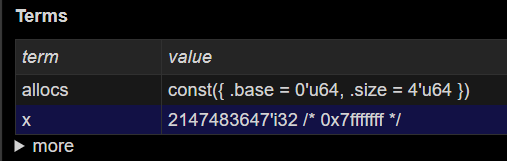
\includegraphics[width=.8\textwidth]{figures/increment_broken_state.png}
    \caption{Counter example for increment\_broken.c.}\label{fig:incr-broken-counter-ex}
\end{figure}

We can avoid this error by constraining the values of the input with a
precondition annotation as follows.

\begin{figure}[h]
    \centering
    \cfile{code/increment.c}
    \caption{Example increment.c.}\label{fig:incr}
\end{figure}

Here we see the keyword \cinline{requires} is used to introduce a pre-condition
on the input. \cinline{MAXi32()} is an in-built function which represents the maximum
value a signed 32-bit integer can represent. By constraining the input so that
it is strictly less than the maxiumum value, the function is now guaranteed to
have no \kl{UB} for all its inputs, no matter what the context. This is because
whilst pre-conditions are \emph{assumed} inside the function, they are
\emph{required} when calling it.

\begin{figure}[h]
    \centering
    \cfile{code/call_increment.c}
    \caption{Example call\_increment.c.}\label{fig:call-incr}
\end{figure}

In the first example, we see that from the constraint \cinline{y <=
100i32},\sidenote{Integer literals are currently written with a type
annotation, similar to Rust.} \kl{CN} deduces that \cinline{y <=
MAXi32()}\sidenote{Foreshadow subtyping, and bidirectional things.} and permits
the call to \cinline{increment}. Conversely, \cinline{INT_MAX} does not meet
that constraint, and so CN raises an error.

\begin{figure}[h]
    \centering
    \cfile{code/decrement_broken.c}
    \caption{Example decrement\_broken.c.}\label{fig:decr-broken}
\end{figure}

However, if we try to decrement the result of the successful call, \kl{CN}
raises an error. This is because that \kl{CN} has no indication on the
constraints of the return value (other than those deduced from its C type,
namely that it fits within a signed 32-bit integer).

\begin{itemize}
    \item Pointers
    \item User defined predicates
    \item Array example
\end{itemize}

\begin{marginfigure}
  \ContinuedFloat*
  \begin{mathpar}
      \inferdef{Var}{\vdash{} \Gamma{} \\ (x: A) \in{} \Gamma{}}{\Gamma{} \vdash{} x \ty{} A}\label{rule:cic-var}
  \end{mathpar}
  \caption{Integrate Ott into this system.}\label{fig:cic-var}
\end{marginfigure}

Reference the rule: \ruleref{rule:cic-var} opposite.

\begin{marginfigure}
\ContinuedFloat{}
  \begin{mathpar}
      \inferrule{\Gamma{} \vdash{} A \ty{} \uni{} \\ \Gamma, x: A \vdash{} t \ty{} T}
      {\Gamma{} \vdash{} \l x: A.\ t \ty{} A \to{} T}
    \and
    \inferrule{\Gamma{} \vdash{} f \ty{} A \to{} T \\ \Gamma{} \vdash{} u \ty{} A }{\Gamma{} \vdash{} f\ u \ty{} T}
  \end{mathpar}
  \caption{Ott in here too.}\label{fig:cic-nondep-fun}
\end{marginfigure}

You can see more at work in \cref{fig:cic-nondep-fun}.

\section{Contributions of this thesis}\label{sec:contributions}

\subsection{Formalisation of CN}

Kernel CN (type safety), the gap between CN and this (inferring output
arguments, historical note on inferring indices), heap factoring, and Ott
engineering.

\subsection{Design, formalisation and implementation of CN-VIP}

Memory object model and adapting it to CN

\subsection{Will the real world C, please stand up?}

Tree Carver (preprocessor), buddy allocator update, issues/pain points (on
GitHub repo), working with Galois.

\begin{comment}

\emph{“\kl{Coq} is an old man now, and it has a lot of scars.”}
\vspace{-1.5em}
\begin{flushright}
  \sidecite[][citing Assia Mahboubi]{QuantaPA}
\end{flushright}

\margintoc[4em]

This thesis belongs to the domain of \kl[dependent type]{type theory},%
\sidenote{If you do not know what this or any other word in this introduction
means, read on! They will be explained in due time.}
itself at the crossroads between computer science and mathematical logic.
One of the field’s goals is to give theoretical and practical foundations
for software tools helping humans in constructing and verifying proofs –
in the mathematical sense.
Such tools are called \kl{proof assistants}, and \kl{Coq}, the one
on which my work was mainly focused, is central in this thesis.

Over their more than 50 years of existence, proof assistants have
turned into an established technology. This history is both a blessing and a curse: as
the field matured, the tools have become more and more complex, making them more and more
powerful, but also more and more prone to critical bugs hiding in dark corners. At a time
when they are gaining traction in an increasing number of communities
concerned with high trust levels, this simply cannot be.
The historical solution of keeping a small, trusted \kl{kernel}
– the so-called De Bruijn criterion –
is not enough if we wish to keep moving on and integrate new, powerful features
to keep up with the needs of users.

There is a straightforward solution to this:
proof assistants have been used for decades to certify programs correctness.
Why could they not prove \emph{themselves} correct? After all, if this is
the gold standard we demand for software, it should apply first and foremost to the ones
used to justify that trust. For the proof assistant \kl{Coq},
this is the ambition of the \kl{MetaCoq} project,
which aims at providing a drop-in replacement for \kl{Coq}’s \kl{kernel} that has been
proven correct,
even though it handles all the subtleties and quirks of said \kl{kernel}.
No more trusting a complex and ever-evolving implementation, trust the formally validated
\emph{proofs} instead!

But before we can hope to achieve that goal, we need a deeper study of the structures at work
in the \kl{kernel}. In particular, its typing algorithm is \emph{bidirectional}, meaning that
it constantly alternates between the two problems of type \emph{inference} –
finding a type for a term – and type \emph{checking} –
verifying that a type is adequate for a term. While this
structure is crucial in relating the specification of the type system to its implementation,
it has been rather little studied in the context of the
\kl{Calculus of Inductive Constructions} (\kl{CIC}),
the theoretical foundation of \kl{Coq} – but also of the closely related
\kl{Lean}, \kl{Agda}…

This thesis aims at filling that gap, by providing a thorough study of bidirectional \kl{CIC},
formalized in the framework offered by \kl{MetaCoq} project. This is a key
ingredient in the first formal proof of soundness and completeness of a type-checking
algorithm for a realistic proof assistant kernel.
It was also able to uncover bugs in \kl{Coq}’s kernel that had gone unnoticed until then.

But bidirectional typing is also an interesting theoretical tool in its own right,
giving a valuable form of control over computation.
In particular, it is a necessary piece in the design of a gradual extension of
\kl{CIC}, \kl{GCIC}.
\kl{Gradual typing} aims at bringing to programmers both the flexibility of
development offered by dynamic typing, and the strong guarantees given
by static typing, in one and the same system. \kl{GCIC} intends
to bring that flexibility to dependently-typed programming,
and, by using the power of the \kl{Curry-Howard correspondence}, to proof writing.
But this endeavour comes with subtle difficulties,
that can only be solved in a bidirectional setting.

To replace this work in its larger context, this introduction begins with a very
short history of mathematical logic (\cref{sec:logic-history}), which exposes the
main questions of that field. Follows a presentation of the links between logic and
computer science, through \kl{proof assistants} (\cref{sec:proof-assistants}).
Next, \cref{sec:intro-coq-en} focuses more closely on presenting
the research questions I worked on: bidirectional typing, \kl{MetaCoq} and gradual typing.
Finally, \cref{sec:this-thesis} summarizes my contributions to these questions.

\section{A Very Short History of Logic}
\label{sec:logic-history}

\subsection{Syllogisms}

The main question that logic seeks to answer is that of finding criteria in order to determine
if a reasoning is valid. In Western tradition, this challenge can be traced back to the
Antiquity, and particularly to Aristotle's \textit{Organon}.
The main contribution of this work is to introduce the notion of syllogism.
These are simple fragments of reasoning, whose validity stems from the
fixed structure they follow, rather than a specific content.%
\sidenote{The most well-known is probably the \textit{Barbara} syllogism, and example
of which is: \emph{all humans are mortals; Socrates is human; so Socrates is mortal.}}
If complex reasoning is built from assembling such syllogisms, it must necessarily be valid as
a whole, since every assembled fragment is. There are two important ideas at work here.

The first is that reasoning can be valid or not, depending only on its structure,
independently of its content.
It can be syllogisms, but many other systems. We will come across a certain number of them
in this thesis!

The second idea is that of a construction from elementary components.
Starting from a set of rules
we have identified as valid \textit{a priori}, we have a means to ensure the validity
of potentially very complex reasoning: it suffices to check that these
can be decomposed into the base components.

For the Greek philosophers, logic was also conceived as a means towards communication.
The aim was to check one’s own reasoning, but also to be able to convey
it, by fixing a logical formal system.%
\sidenote{Structural rules reasoning should obey, as those of syllogisms.}
A person wanting their conclusion to be accepted by others would only have to express their
reasoning in a perfectly precise way in the framework of such a formal system.

From that point on, the main focus of logic as a discipline
concentrates on this structure which underlies reasoning.
The main challenge is to construct a formal system, adapted to a specific
field of reasoning. In the case we are interested in, mathematical logic, this
allows us to give a precise meaning to what constitutes a valid mathematical proof.


\subsection{The beginning of mathematical logic: towards a formal foundation}[Towards a formal foundation]

Following Aristotle, mathematicians seized logic in order to build a formal system
able to serve as a rigorous foundation for mathematics.
The links between logic and mathematics go back to Greek Antiquity, but
mathematical logic as a standalone discipline really established itself
during the 19\textsuperscript{th} century, thanks to important progress on two main aspects.

The first consisted in freeing mathematical logic from natural languages%
\sidenote{By opposition with the formal languages which appear in mathematics,
  computer science, etc.},
unsuited to a formal description of reasoning, and to instead design a new specific
form of language that could serve as a basis for mathematical reasoning.
An important step here was \citeauthor{Begriffsschrift}'s
\citetitle{Begriffsschrift}~\sidecite{Begriffsschrift}, which, for the first time,
gave a formal language rich enough to express mathematics satisfyingly. Its
major addition was the notion of quantifier, essential to the mathematical vernacular,
as they give a faithful way to account for universal%
\sidenote{For instance: “Every even natural number is the sum of two prime numbers”.}
and existential%
\sidenote{For instance: “There exists a real whose square is 2”.}
properties.

The second aimed at showing that mathematics as a whole could be reconstructed from a
few simple properties. An important step was the reduction of analysis to the properties
of real numbers, followed by constructions of those from arithmetic given almost
simultaneously by – among others – \sidetextcite{Dedekind1872} and
\sidetextcite{Cantor1872} in 1872.
Meanwhile, \sidetextcite{Peano1889} proposed an axiomatization of natural numbers close to the
one still used today. Finally, Cantor again proposed set theory \sidecite{Cantor1883}
as a formalism expressive enough to describe all mathematical object as sets of elements.

\subsection{The foundational crisis of mathematics}[The foundational crisis]

Unfortunately, the system proposed in the \citetitle{Begriffsschrift} is inconsistent!
That is, it is possible to use it to prove falsity, 
making the logical system collapse.%
\sidenote{In a system where falsity is provable, all propositions are,
  which is known as the principle of explosion.
  Such a system, where everything – and its negation – is provable can obviously not
  serve as an adequate foundation for mathematics.
}
This result, due to Russell%
\sidenote{%
  In a letter to Frege in 1902 the latter made made public
  in \textcite[Nachwort p.~253]{Frege1903}.}%
\margincite{Frege1903}
marked the opening of a crisis period.
Indeed, it cast doubt upon the systems that had started to establish
themselves as good candidates to serve as foundations – that of Frege, but
mainly those of Cantor, which were affected by the same difficulties.

A possible solution has been suggested ten years later  by \citeauthor{Whitehead1913} in their
\citetitle{Whitehead1913} \sidecite{Whitehead1913}. This colossal piece of work
not only proposed a formal system avoiding the inconsistency
of \citetitle{Begriffsschrift}. It also built a significant amount
of mathematics in this system, including a construction of integers,
some arithmetic, and finally real numbers.

In parallel, in the continuity of Cantor’s work, \sidetextcite{Zermelo1908} and others
worked towards giving a version of Cantor’s set theory that is consistent. This lead to what
is colloquially referred to as Zermelo-Fraenkel set theory – ZF, or ZFC when the
axiom of choice%
\sidenote{An axiom very useful in numerous branches of mathematics, but which is often treated
separately, as it is both less crucial than the other axioms of ZF and at the root of
counter-intuitive results.}
\sidecite{Zermelo1904} is added –, which also seemed able to serve as a
solid foundation for mathematics.

\subsection{Incompleteness}

The search for a formal system adequate as a foundation for mathematics however hit a
second major difficulty: Gödel’s incompleteness theorem \sidecite{Goedel1931}. It asserts
that a formal system in which one can construct integers such as those of Peano – and so
\textit{a fortiori} any system rich enough to serve mathematician’s needs – cannot
prove its own consistency.%
\sidenote{Unless the system is inconsistent, in which case it can prove \emph{everything},
by virtue on the explosion principle, including its own consistency… and inconsistency!}
Thus, no formal system can serve as a basis for mathematics
with a formal certitude as to its adequacy.
Indeed, as we cannot prove the consistency of the system in itself, it could very well
turn out to be inconsistent, ruining all the efforts put into its use – just like what
happened with Frege’s \citetitle{Begriffsschrift}. And if we were to use a second system
to prove the first consistent, we would only shift the prolem: now we rely on the
consistency of the second system.

A consequence of this theorem is that a system rich enough to found mathematics is
necessarily incomplete.%
\sidenote{%
  This means that there exist independent statements, that is assertions which
  cannot be proven, and whose negation cannot be proven either.
  The consistency of the system under consideration is one example of such a statement.
}
Thus, in what follows, I will never refer to truth in an absolute sense – which could
only be meaningful in a complete system where every statement is true or false –, but
only about provability \emph{relatively to a given system}.

\subsection{A satisfactory situation?}

Despite the difficulties put into light in the beginning of the 20\textsuperscript{th}
century, the research in mathematical logic reached a somewhat satisfactory situation
a few decades later.
First, ZFC is a reasonable formal system on which mathematics can be founded. Moreover,
the mathematical community is overall convinced it would be \emph{theoretically} possible
to write down all mathematics using ZFC\@. This is enough for most of its members,
even if those who attempt to actually give it a try, in the vein of the
\citetitle{Whitehead1913}, are quite few.

In \emph{practice}, however, things are very different. The human development and
verification of formalized mathematics%
\sidenote{%
  That is, effectively expressed in a fixed formal system.}
seems both impossible, and unnecessary.
On the one hand, it would demand a considerable effort, because such mathematics would
require an extremely high level of precision, both from the author of the formal proof
and from the reader. At the same time, this would not significantly reduce the risk of
errors. It would indeed be very hard for humans to check that some reasoning doubtlessly
follows the rules of the system: a tiny error can easily creep inside thousands of pages
of formal reasoning. Finally, describing mathematics in this way would drown the vital
mathematical intuitions, making communication sterile.

If we wish to make formal mathematics practicable, and benefit from the guarantees
they bring while eliminating these crippling defaults, we thus need new tools.

\section{Computers Enter the Scene}
\label{sec:proof-assistants}

A new element however radically modifies the previous situation: the advent of computers.
Indeed, computer science provides new tools, making formalized mathematics both possible
and attracting.

\subsection{Proof assistants}

Computers excel where humans are weak: their speciality is to treat large volumes of
information in a very precise way, exactly the kind of needs brought up when manipulating
formalized mathematics. Therefore, already at the beginning of the 70s,%
\sidenote{With systems like Automath \cite{DeBruijn1970}, or Mizar
  \cite{Rudnicki1992}.}%
\margincite{DeBruijn1970}%
\margincite{Rudnicki1992}
software tools, collectively called \intro{proof assistants}, start to
appear, that are dedicated to writing and verifying formal proofs.
Through the formalization of proofs and the verification by computers that they
actually follow the rules of the underlying logical system, proof assistants open the
door to a level of trust much higher than that allowed by “informal” proofs.
Renowned mathematicians, such as \sidetextcite{Voevodsky2010},
\sidetextcite[][Preface, p.\ xi]{Hales2012}, or \sidetextcite{Scholze2021} have indeed
turned to proof assistants, particularly in order to lift uncertainties regarding the
solidity of their own work.

Moreover, proof \emph{assistants} are not simply proof checkers: beyond verification,
they supply users with a large range of tools to ease the conception of
formal proofs. These tools allow users to write proofs at a
high level, and in an interactive manner,%
\sidenote{In most modern proof assistants, the final proof is built as the result of
  an exchange between the programmer and the tool, rather than written as a single block.}
leaving it to the proof assistant to construct the formal proofs.
They range from simple facilities, such as the possibility to visualize the structure
of proofs, or the tracking of hypotheses, to much more ambitious techniques.

Indeed, computer science lets us automatize entire parts of
proof writing, for instance through the use of tactic languages \sidecite{Delahaye2000},
with which one can program proof generation.
In addition, the automatic construction of proofs is a research field by itself,
and the question of its integration intro proof assistants is an active topic
\sidecite{Blanchette2016,Ekici2017}. Computer science has also proven its worth in the
setting of mathematical computations (computer algebra systems, numerical analysis),
and here again promising interactions with proof assistants are starting to arise
\sidecite{Lewis2022,Mahboubi2019}.

Finally, if the use of software eases the writing of proofs, proof assistants conversely
open new possibilities for programming. They indeed offer a natural framework to describe in
the same place the source code of a program, its specification, and the formal proof that the
former fulfils the latter. This way, we can \emph{prove} that the program runs correctly,
without encountering any bugs.
This mathematical certainty is much more reliable than any test set!
In this field, numerous projects have already achieved large scale programs, entirely proven
correct: compiler for the C language \sidecite{Kaestner2017}, implementation of the
\textsc{Https} protocol \sidecite{Bhargavan2017}, differential equations solving
\sidecite{Immler2018}…

\subsection{Logic, Programming and Type Theory}

In order to work, proof assistants must be founded on a formal system, corresponding to
the “rules” of the mathematical “game” they are supposed to enforce.
Thus, they require a renewed study of mathematical logic, but with the practical aim of
building tools that are at the same time powerful and easy to use.
There are multiple families of proof assistants, based on very different formal systems.
The one I am interested in in this thesis relies on the \kl{Curry-Howard correspondence}
and \kl[dependent type]{dependent type theory}. The proof assistant \kl{Coq}
\sidecite{CoqDevelopmentTeam2022}, which is at the heart of my work, belongs to this family.

If one compares a computer program with a text in a natural language,
\intro(en){types}
are a kind of equivalent of grammatical categories. However, contrarily to natural
languages, these types are conceived at the same time as the programming language, in order
to mirror properties of the objects it manipulates.
Their first use is to detect manifest errors. For instance, if a procedure
intended for an object of type “image” is applied to an object of type “character string”,
an error can be reported to the programmer.%
\sidenote{A well-known slogan due to \textcite{Milner1978} claims that
“Well-typed programs cannot go wrong.”}%
\margincite{Milner1978}
But types are very versatile, and their capacity to encode properties of the underlying
programs can be used for compilation, documentation, and many other applications. In our
framework, for instance, types correspond to the validity of a logical reasoning.

This idea is that of the \intro{Curry-Howard correspondence}.%
\sidenote{Made explicit for the first time in informal notes by Howard dating back to 1969,
but published only much later \cite{Howard1980},
themselves based upon previous remarks by Curry \cite{Curry1958}.}%
\margincite{Howard1980}%
\margincite{Curry1958}
Rather than a precise theorem,
it is more of a very general concept, according to which two worlds closely resemble each
other: on the one hand, that of logic and proofs, on the other that of programs
and their types.

\begin{marginfigure}

  % \begin{mathpar}
  %   \inferrule{ \Gamma, A \vdash B}{\Gamma \vdash A \Rightarrow B} \and
  %   \inferrule{\Gamma \vdash A \Rightarrow B \\ \Gamma \vdash A}{\Gamma \vdash B} \and
  %   \inferrule{\Gamma, x : A \vdash t : B}{\Gamma \vdash \lambda x : A . t : A \to B} \and
  %   \inferrule{\Gamma \vdash f : A \to B \\ \Gamma \vdash u : A}{\Gamma \vdash f~u : B}

  % \end{mathpar}

  % \caption{Règles d’inférence pour l’implication et de typage des fonctions}

  \begin{mathpar}
    \inferrule{A \\ B}{A \wedge B} \and
    \inferrule{A \wedge B}{A} \and
    \inferrule{A \wedge B}{B} \\
    \inferrule{a \ty A \\ b \ty B}{(a,b) \ty A \times B} \\
    \inferrule{p \ty A \times B}{p.1 \ty A} \and
    \inferrule{p \ty A \times B}{p.2 \ty B}
  \end{mathpar}
  
  \caption{Inference rules for conjunction and typing rules for pairs}
  \label{fig:curry-howard-example-en}
\end{marginfigure}

A short example says more than a long abstract talk, so let’s look at the correspondence
at work in \cref{fig:curry-howard-example-en}, in the form of inference/typing rules:
each bloc presents a rule, with above the bar the hypotheses, and below the conclusion.
The first three rules govern the logical conjunction “and”, written $\wedge$.
The first means that to deduce the proposition $A \wedge B$ (“$A$ and $B$”), it is enough
to deduce $A$ and $B$ taken individually.
Conversely, if we have as hypothesis $A \wedge B$, then we can deduce both $A$ (second rule),
and $B$ (third rule).
The last three rules govern typing%
\sidenote{Written using a colon.}
for the pair type $A \times B$. A pair $(a,b)$ built
from a first object $a$ of type $A$ and a second object $b$ of type $B$ has type $A \times B$.
Conversely, if $p$ is a pair of type $A \times B$, then we can retrieve its first component
$p.1$, which is of type $A$, and its second $p.2$, of type $B$.
If we erase the terms%
\sidenote{In the context of type theory, we often talk about \emph{terms} instead of programs,
  but the two are synonyms.
}
of the bottom rules, we obtain \emph{exactly} the rules above!
Thus, the programming construct of pairs corresponds to the logical concept of conjunction.

This extends well beyond the specific case of conjunction, in a general correspondence
between, on one side, logical propositions and their proofs, and, on the other, types and programs.
We can see properties as types, and a proof of a given property as a program of the
corresponding type – or the other way around!
Beyond a simple analogy between formalisms of different origins, this correspondence
is a powerful tool to establish a dialogue between two worlds. In particular, it
relates two \textit{a priori} quite distant problems: checking that a proof
is valid, and checking that a term is well-typed. In both cases, it amounts to checking that
a construction – program on one side, proof on the other – respects a set of formal
rules guaranteeing it is well-formed.

The \kl{Curry-Howard correspondence} is therefore ideal to serve as a foundation for
\kl{proof assistants}, since it gives access, when studying formal logical systems,
to the rich literature on programming languages, in particular on the theory and
implementation of types. In this framework, the
\intro[dependent types]{dependent type systems} are a specific family of type systems,
whose main characteristic is the ability for types to depend on terms. The archetypical
example from the point of view of programming is the type $\Vect(A,n)$
of vectors of length $n$. These are lists that contain exactly $n$ elements of type $A$ – with
$n$ a natural number.
This type depends on $n$, in the sense that the type’s inhabitants differ depending on the
integer’s value.
From the point of view of logic, this dependency corresponds to quantification: if we
wish to express a universal property “for all $x$, the property $P(x)$ holds”, then we need
the property $P$ to depend on $x$.
Thanks to this ability to express quantification, dependent types are rich enough
to serve as foundations for mathematics.

\section{\kl{Coq} and Its Kernel}
\label{sec:intro-coq-en}

Let us now focus a bit more on the proof assistant which we will consider mainly in this
thesis: \kl{Coq}.

\subsection[The kernel]{The kernel, cornerstone of the system}

\begin{figure}[h]

  \centering
  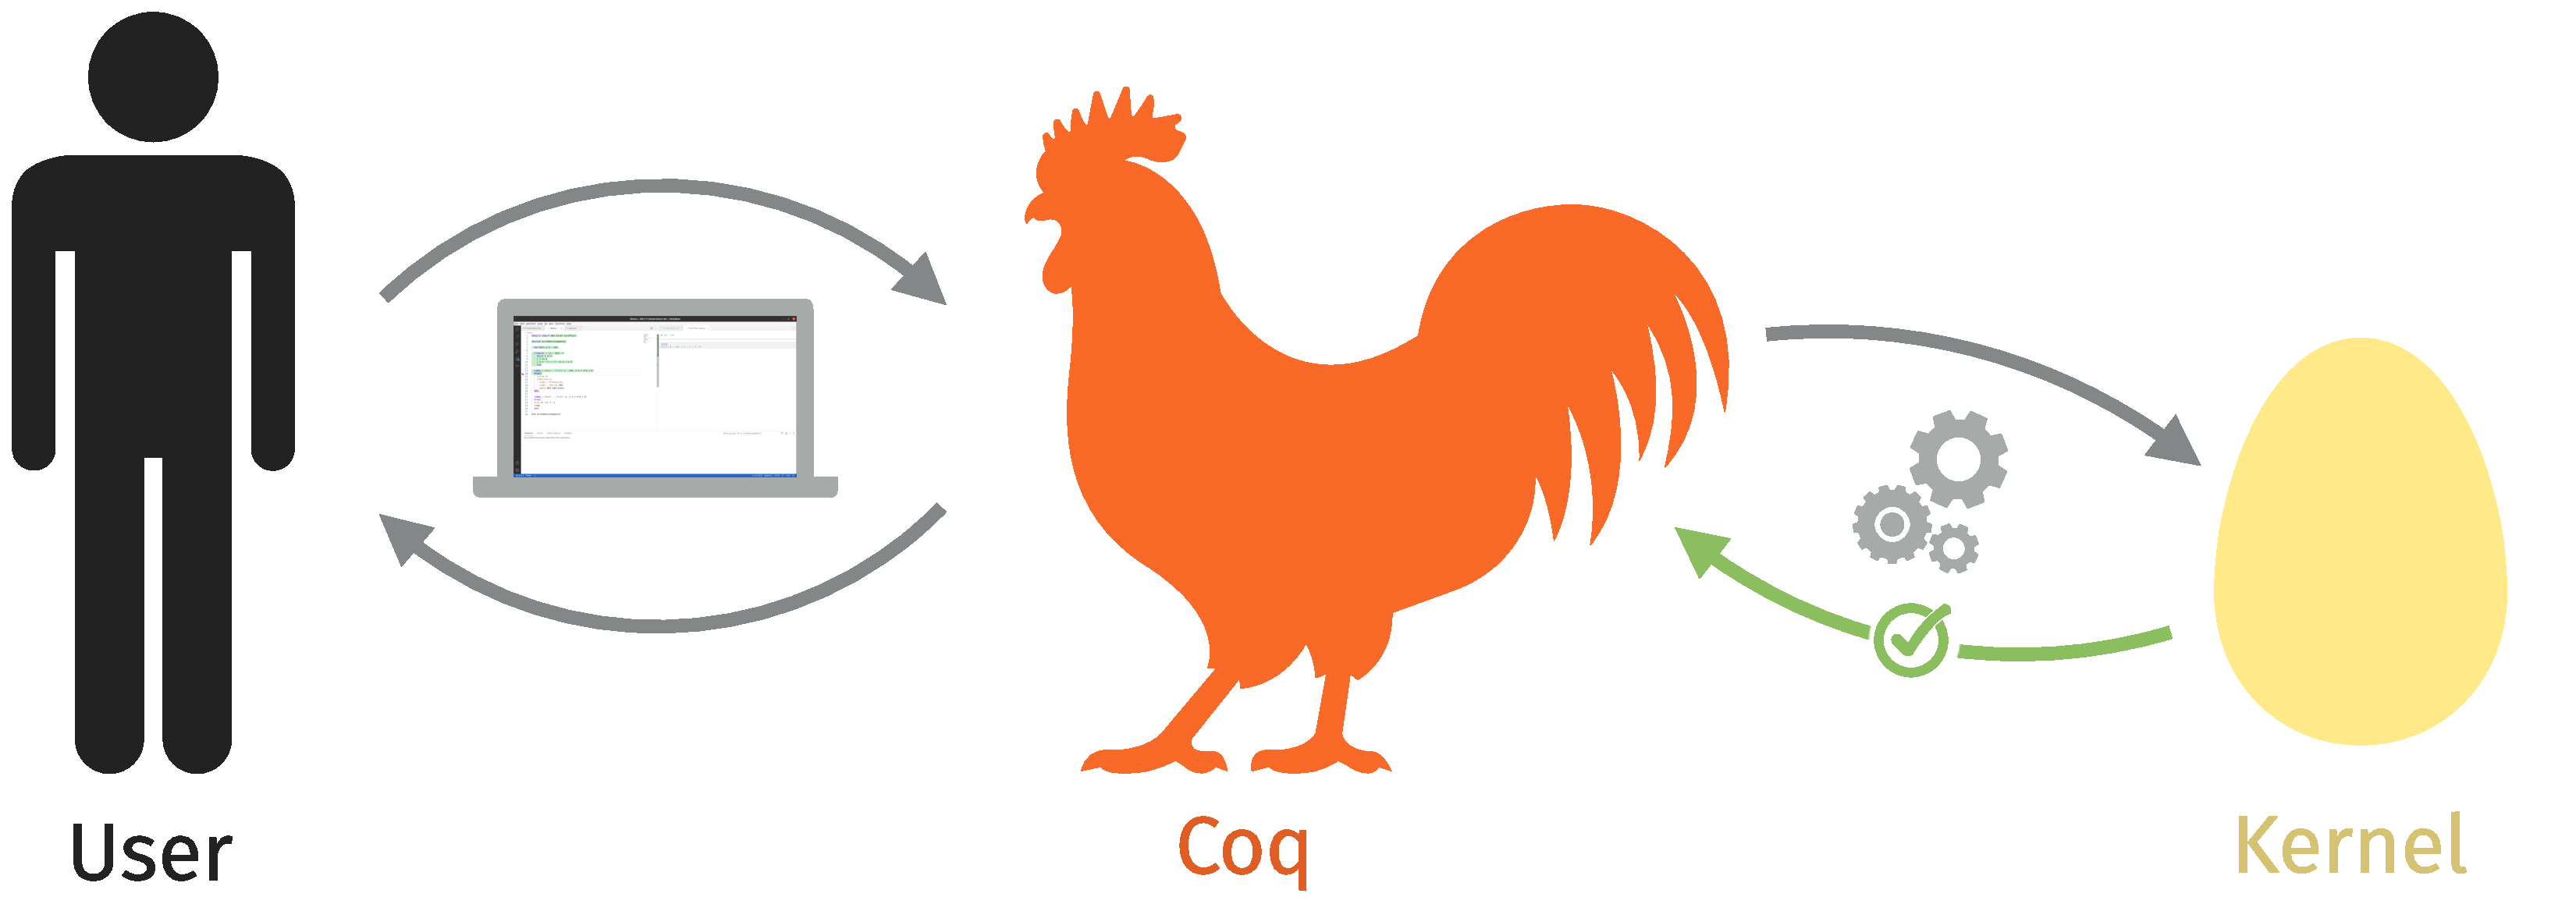
\includegraphics{./figures/coq-kernel-en.pdf}

  \caption{\kl{Coq}’s schematic architecture}
  \label{fig:coq-en}
\end{figure}

\kl{Coq} is based on the \kl{Curry-Howard correspondence}: proofs are seen as programs,
in a language called \intro{Gallina}, and their verification is done using an algorithm
close to those used for types in conventional languages. However, if, in the first versions
from the 80s, \kl{Coq} proof were mostly written directly in \kl{Gallina}, it is
no longer the case at all. The reason is that the major part of the tool in its
current versions aims at helping the user in generating a correct proof. It is a true
\kl[proof assistant]{proof \emph{assistant}}!
The way \kl{Coq} works is illustrated in \cref{fig:coq-en} : the user interactively exchanges
with \kl{Coq}, which uses this interaction to generate a proof term. This proof term is then
sent to a very specific part of the tool, called the \intro{kernel}.
This is the part implementing the type-checking algorithm, and thus responsible for ensuring
that the proof terms built interactively are correct.
The \kl{kernel} is thus the crucial part of \kl{Coq}, because it is the one – and only –
ultimately responsible for proof-checking.
This architecture, which clearly isolates the critical part of the system, is called
\intro{De Bruijn criterion} \sidecite{Barendregt2001}, in tribute to one of the pioneer
of proof assistants.

If the rest of the ecosystem has grown much more than the \kl{kernel} since the beginning,
the latter has also evolved, becoming gradually more complex.
And, as any other software development, it is not safe from bugs.%
\sidenote{The magnitude is that of one critical bug found every year, a list is maintained
at the following address: \url{https://github.com/coq/coq/blob/master/dev/doc/critical-bugs}.}
These are in general hard to exploit for a user, even more so without noticing.
But still, they exist, and since the \kl{kernel} tends to get more and more complex, they
are likely to continue appearing.

\subsection{\kl{MetaCoq}, a formalization in \kl{Coq}, for \kl{Coq}}[\kl{MetaCoq}]
\label{sec:intro-metacoq-fr}

If we wish to guarantee a trust level as high as possible in the \kl{kernel}, we must
resort to new ideas. This is what the \kl{MetaCoq} project is all about. The idea
is simple: use \kl{Coq} itself to certify the correctness of its \kl{kernel}.

More precisely, the first step is to describe formally the type system on which the \kl{kernel}
is based, and to show its theoretical properties.
This is already a difficult endeavour: in order to ease its use, \kl{Coq}’s type theory
incorporates a lot of complex features.

Once this meta-theory is established, the second step
% \sidenote{This is the one on which I mostly work, and on which we will come back in more
% length later on.}
consists in implementing a type-checking algorithm as close as possible to the one of the
\kl{kernel}, directly in \kl{Gallina}%
\sidenote{Indeed, thanks to the \kl{Curry-Howard correspondence}, \kl{Gallina} is not
only a proof language, but also a true programming language!}.
We show, while defining the algorithm, that it is indeed \reintro(bidir){sound}%
\sidenote{If the algorithm claims that a term is well-typed, then it is the case.}
and \reintro(bidir){complete}%
\sidenote{The algorithm answers positively on all well-typed programs.}.
Together, these two properties correspond to the \intro(bidir){correctness} of
the program.

Finally, in a third step, we extract out of this certified \kl{Gallina} program another
more efficient program, by erasing the content related to the proof of correctness, in order
to keep only the algorithmically relevant one.
This extraction is a complex but crucial step if we wish to replace the current \kl{kernel}
while keeping a reasonable efficiency. Therefore, we also prove that said extraction
is correct,%
\sidenote{Meaning that it preserves the semantics of programs.}
once again by programming it in \kl{Gallina}.

\subsection{Checking, inference and bidirectional typing}[Bidirectional typing]

While proving the correctness of the type-checker is relatively easy once the
meta-theoretical properties of the type system have been established, completeness is harder.
In order to prove it, it is very useful to go through an intermediate specification,
which is more structured than the theoretical one.
In particular, it is important to separate two close but distinct questions:
on the one side, type-checking, where we \emph{check} that a term indeed has a
given type;
on the other side, inference, where we try and \emph{find} a type for a term, if such a
type exists.
The typing algorithm of \kl{Coq}'s \kl{kernel} is \intro{bidirectional}, meaning that it
alternates constantly between these two processes when it checks that a term is well-typed.
Describing this bidirectional structure independently of the algorithm allows for a
clear separation between, on the one side, its equivalence with the original specification,
and, on the other, the part purely dedicated to implementation questions.

In the specific case of dependent types, even if present in type-checking algorithms since
the origin – see \eg \sidecite{Huet1989} –, bidirectional typing has been relatively little
studied. However, beyond its strong relation to algorithms, this approach also presents
theoretical advantages: its more constrained structure makes it easier
to obtain properties that are difficult to obtain in the standard context.

\subsection{Gradual types: some flexibility in a desperately static world}
  [Gradual types]
\label{sec:intro-graduel-en}

There are two main approaches to program type-checking. In the static approach,%
\sidenote{On which \kl{Coq} is based.}
types are verified prior to the execution, whereas, in the dynamic approach, the well-typedness
of operations is verified on the fly during that same execution.
The dynamic discipline is more flexible, as it checks exactly what is necessary
for the good execution of a program.
The strictness of static typing, conversely, allows for error detection earlier in the
development, and imposes invariants useful to optimize compilation or execution.

Instead of opting exclusively for one of the two approaches,
\reintro{gradual typing} \sidecite{Siek2015} aims at integrating
the static and dynamic disciplines in one and the
same language.
The main idea is to have a first pass of verification before the execution, as in static typing,
while leaving the possibility to defer parts of the verification to the execution, as in
dynamic typing.
This gives access to a whole spectrum of options, from a rigid completely static
discipline to a flexible dynamic one. It particularly allows for a fine-grained, local choice
of how each part of a program is type-checked.
One can thus evolve the discipline during software development, benefiting from
the flexibility of dynamic typing in early phases, and from the guarantees of static typing
later on.

As the case of \kl{MetaCoq} illustrates, \kl{Coq} can be used as a true programming language.
Even better: its type system can express very complex properties of programs, and thus
verify even before their execution that the code indeed enforces them.
Sadly, these reinforced constraints can turn against the user, by making the
early development phase more difficult. Indeed, nobody writes correct code on the first try,
and it would often be nice to temporarily lift the strong guarantees of typing to
facilitate experimentation. The idea then is to take inspiration from gradual typing,
in order to pave the way for a more flexible logical or software development. Once again, the
\kl{Curry-Howard correspondence} is at work, since we adapt concepts from the world of
programming languages to the logical one.

\section{And this Thesis?}
\label{sec:this-thesis}

My doctoral work itself is centred around bidirectional typing, under three main aspects,
corresponding to the three parts of this thesis.
They are preceded by \cref{chap:tech-intro}, which introduces the main technical notions
used in what follows.

\subsection{Theory of bidirectional typing}

The first part (\nameref{part:bidir}) proposes to – partially – fill the theoretical gap around
bidirectional typing for dependent types. More precisely, it contains a proof of equivalence
between the standard presentation of CIC in the literature, and a bidirectional one.
\Cref{chap:bidir-ccw} presents the main ideas in a relatively
simple setting, in order to ease the exposition. \Cref{chap:bidir-pcuic} shows how to extend
them to a more realistic setting, close to the type theory implemented in \kl{Coq}.
Finally, \cref{chap:bidir-conv} focuses on the particular status of conversion%
\sidenote{This crucial notion allows the integration into dependent type theory of
the notion of computation of programs.},
and the links between recent work on this subject and bidirectional typing.

\subsection{Bidirectional typing in \kl{MetaCoq}}

The second part of the thesis (\nameref{part:metacoq}) focuses on the \kl{MetaCoq} project,
and especially the formalization, in \kl{Coq}, of the ideas presented in the first part.
\Cref{chap:metacoq-general} gives a general overview of the project, while
\cref{chap:kernel-correctness} concentrates more specifically on the proof that the
\kl{kernel} implemented in \kl{MetaCoq} fulfils its specification.

\subsection{Gradual dependent types}

Finally, the third and last part (\nameref{part:gradual}) presents my work in the area
of \kl{gradual types}. Since dependent types already form complex systems, their adaptation
to the gradual approach is particularly delicate. A summary of the possibilities and issues is
presented in \cref{chap:gradual-dependent}. An interesting point of emphasis is that the
usual presentation of dependent types turns out to be unsuited, as it is too flexible.
The additional structure provided by bidirectional typing is key to solve this issue. It is also
relevant to present the type-directed elaboration of terms from a source language
to a target one, an important characteristic shared by all \kl[gradual types]{gradual languages}.
The use of a bidirectional elaboration, and the properties it allows us to obtain, are described
in \cref{chap:bidir-gradual-elab}. Finally, \cref{chap:beyond-gcic} describes follow-up work
complementing that of \cref{chap:bidir-gradual-elab}, but which is not directly linked to
bidirectional typing.

\subsection{Technical contributions}

My doctoral work started with the study of \kl(typ){gradual}
\kl(typ){dependent} types.
I contributed, together with Kenji Maillard, Nicolas Tabareau and Éric Tanter, to
\sidetextcite{LennonBertrand2022}, where we study a gradual extension to the
Calculus of Inductive Constructions. My main technical contribution corresponds
to \cref{chap:bidir-gradual-elab}. The precise literature review and the impossibility
theorem of \cref{chap:gradual-dependent} it leads to also comes from this
publication.
The second technical part of \textcite{LennonBertrand2022}, in which I participated but
whose main author is Kenji Maillard, as well as a second article,%
\sidenote{\textcite{Maillard2022}, currently under review.}%
\margincite{Maillard2022}
together with the same authors and again Kenji Maillard as main investigator,
correspond to \cref{chap:beyond-gcic}.

This work having shown the relevance of a bidirectional dependent type system and the relative
scarceness of results on the subject, I focused more closely on it, both on
paper and by means of a formalization based on \kl{MetaCoq}. This led to a second publication
\sidecite{LennonBertrand2021}, and corresponds to \cref{chap:bidir-ccw,chap:bidir-pcuic}
for the theoretical part, and \cref{sec:kernel-bidir} for the formalized proof
of equivalence between bidirectional and undirected typing.
The completeness bug in the kernel of \kl{Coq} found during this formalisation, together with
the impact of this discovery on the implementation of \kl{Coq} is presented in
\sidetextcite{Sozeau2022}.

I then turned to the closer integration of this formalization into \kl{MetaCoq}, and its use
in order to prove completeness of the \kl{kernel} it implements.%
\sidenote{A definition of a type-checking algorithm proven sound but not complete by
Simon Boulier was already present, although I had to alter it during the completeness
proof.}
This is described in \cref{sec:kernel-typing}.
I also contributed more generally to the project on various more minor points.
This part of my thesis work has not been published yet, but the other contributors to
\kl{MetaCoq} and I are currently working on it.

Finally, \cref{chap:bidir-conv} corresponds to a project I initiated in order to extend
\kl{MetaCoq} to integrate extensionality η rules to conversion,
but which did not reach the stage of publication yet. Yet, I presented the difficulties
that led me to it in \sidetextcite{LennonBertrand2022a}.

\end{comment}


\pagelayout{wide} % No margins
\addpart{Formalisation}%
\label{part:formalisation}
\pagelayout{margin} % Restore margins

In the \cref{sec:c-lang}, I discussed how competing forces of inherited
portability requirements, proximity to hardware, and the desire for more
aggressive optimisations led to complex and subtle technical resolution by
stakeholders in the \kl{ISO} standard of C. I also mentioned that its nature as
a prose document, with natural language ambiguities and omissions, as well as
divergence C as used \kl{de facto}, mean that its semantics are unreasonable
for a human to adhere to, and challenging to build into tools directly,
without making some sort of simplifying assumptions.

Existing program logic frameworks for C such as Verifiable C~\sidecite{appelSF5}
and RefinedC~\sidecite{sammler2021refinedc} take the approach of building a
logic directly above an operational semantics for a language which is
recognisably C, minus some desugaring to consolidate similar constructs. They
attempt to retain as many C features (control flow, variable scoping, aliasing,
loose evaluation order, pointer manipulation rules) as possible, but make
simplifying assumptions where it would be impractical otherwise.

Given that \kl{CN}'s headline goal (\cref{sec:cn-intro}) is to work with
pre-existing C programs, which rely on many if not all of those impractical
features, adopting the conventional approach would quickly use up most of its
complexity budget and make the other goal (of reducing the expertise required
to do verification) unfeasible.

Instead, \kl{CN} builds directly upon the
\kl{Cerberus}~\sidecite{memarian2022cerberus} executable and empirically
validated semantics for C. Not only does \kl{CN} benefit from the
\emph{accurate} semantics for both \kl{ISO} and \kl{de facto} C, it benefits
most from the \emph{usability} of it. This is because, Cerberus is elaborated
into a relatively small calculus \emph{\kl{Core}}, which translates all of C's
complexity into a first-order functional language with a few special (but easy
to understand and specify) constructs.

Additionally, \kl{CN} is intended to be used more like a \emph{type system} in
an IDE than a program logic inside a proof assistant. Ideally, instead of
seeing intermediate goals in a sophisticated separation logic, and needing to
be well versed with a range of inference rules and automation tactics, a user
sees their C program, scattered with predictable and lightweight annotations in
comments, in an editor which either indicates success, or clear and helpful
error message.

Aside from the fact that the notion and mode of use of a type system is more
familiar to most programmers (an advantage not to be scoffed at), this approach
also allows \kl{CN} to use and advance the extant literature on building
refinement type systems on top of existing languages.

This type system approach also leads to other desiderata and their
corresponding responses. If we want to follow a type system approach, we want
to minimise obvious annotations and justify why the necessary ones are so, we
need to track carefully the flow of information in the type system, using a
\kl{bidirectional} approach. We also need some sort of automation so as to not
burden the programmer with proving things like $1 + 1 = 2$. Similar to
VeriFast~\sidecite{jacobs2011verifast} and Frama-C\sidecite{kirchner2015frama},
\kl{CN} enlists the support of SMT solvers to mitigate this. When trying to
verify code against expressive specifications, this could lead to
non-termination, so \kl{CN} also restricts the expressiveness of the assertion
language, and the queries it sends to the SMT solver. And given the importance
of managing resources in C, the typing discipline needs to be substructural.

The \kl{CN} assertion language syntax aims to be expressive enough to verify
real world C, but also restricted enough to limit the aforementioned technical
problems, and intuitive enough to a target audience of systems programmers who
happen to know Haskell (or Rust).

With this many constraints and design decisions, it is easy to doubtful of the
elegance and feasibility of this approach, let alone consider proving such a
type system sound. As I will show in \nameref{chap:kernel-cn}, whilst the setup
might be novel, multi-faceted and large, the definitions are relatively
straightforward, and the proof of soundness can be done syntactically. Both the
definitions and the proof are modular with respect to the heap, so that
changing the memory object model does not require redoing the entire soundness
proof. The formalisation is close enough to the surface syntax of \kl{CN} so
that a correspondence between the two can be stated simply and precisely, and
close enough to the implementation to offer actionable insights.

\chapter{Formalisation Background}%
\label{chap:formal-background}

\margintoc{}

The components of \intro{Kernel CN} all have precedent in prior work; the main
new contribution is the adaptation and confluence of those ideas. This chapter
will set out \kl{CN}'s design goals and origins, recapitulate the disparate
concepts used in CN, and along the way discuss how they satisfy the
aforementioned design goals.

\section{\kl{CN} Design goals and constraints}%
\label{sec:cn-goals}

Aiming for \emph{``a verification tool whose aspirational goal is to lower the
cost of C verification from a Rocq programmer who knows separation logic to a
systems programmer who knows Haskell''} (\cref{sec:cn-intro}) helps narrow
down the large design space of verification tools.

The reason for picking this particular goal is in \kl{CN}'s origins as
an attempt to verify the pKVM hypervisor, developed by Google.

Before I explain pKVM, I need to explain the context for this. The Android
operating system runs on billions of devices worldwide, playing a central role
in many lives, including handling an enormous amount of sensitive data. This
means that security is paramount, however because each device runs its own
kernel (up to half the code is not Android's version of Linux), updates are
very challenging and expensive to test and deploy to each device. Aside from
security issues, this also leads to fragmentation of Android, so devices and
apps are not all up-to-date and the long delay (at least 18 months) between
Linux and device releases makes to difficult upstream features and fixes.%
\sidenote{%
TODO: cite these properly.
\begin{itemize}
    \item \url{https://youtu.be/7novnkldMmQ?feature=shared}
    \item \url{https://youtu.be/wY-u6n75iXc?feature=shared} and \url{https://lwn.net/Articles/836693/}
    \item \url{https://source.android.com/docs/core/architecture/kernel/generic-kernel-image}
    \item \url{https://source.android.com/docs/core/virtualization/whyavf}
    \item \url{https://googleprojectzero.blogspot.com/2020/02/mitigations-are-attack-surface-too.html}
    \item \url{https://lpc.events/event/7/contributions/780/}
\end{itemize}
}

Whilst some of this has been mitigated with the introduction of
\intro[GKI]{Generic Kernel Images (GKI)}, which provide a small and stable
kernel ABI \emph{for a particular long-term release} version of Android, there
are still security issues present in this model, because the kernel is too
large (20 million lines of code) to be a reasonable trusted computing base, and
the drivers vendors ship with a device are part of it.

Some manufacturers use hypervisors, which attempt to isolate the kernel from
the rest of the system by running Android and other hardware components in
virtual machines, such `secure' parts of the device storing sensitive data.
Aside from security, hypervisors are also used to partition memory at boot-time
so that devices can use it for things like direct memory access, and run
arbitrary code outside of Android, which is worrying because this code would
run at a more privileged level than Android itself. All of this just
\emph{shifts} the attack surface, and has also resulted in \emph{more}
fragmentation at the hypervisor layer.

Similar to GKI, the proposed solution to standardise the hypervisor used. There
is already a mature hypervisor which is part of the Linux kernel, the
Kernel-based Virtual Machine (KVM)\@. It is set up so that a host kernel can
dynamically allocate virtual machines for guests to run on, and protect the
host from the guests. However, at the start of the project, the API exposed by
the hypervisor to the host kernel offered too much control, and guests were not
protected from the \emph{host}. This is a problem because the guest could be
running code for a secure hardware component (e.g.\ a biometric authenticator),
the host could be a compromised version of Android, so an attacker could still
get access to sensitive information.

To solve this, Google, as part of the Android Virtualisation Framework, is
developing a \intro[pKVM]{protected KVM (pKVM)}, which runs \emph{underneath}
the kernel, and ships \emph{as part} of the kernel image. Not only does this
tight coupling remove issues around ABI compatibility between the hypervisor
and the kernel, since the source is always in the same repository, it also
allows pKVM to commit to only handling implementing a select few functions such
as virtual memory management and remain very small, and rely on the Linux
kernel to manage the rest, such as scheduling, device drivers and power
management.

If successful, this could make the attack surface a lot smaller, but it could
also make it one that is used very widely. It is in this context that Google
sought assistance from the research community to see if verifying the kernel
was feasible, \emph{on an ongoing basis}. A one-and-done verification of pKVM
which takes an army of PhD students and postdocs a few years to verify and is
years out of date by the time is developed is not worth the investment, a
tool which C kernel hackers can understand, use and maintain proofs as they
make changes to very important security critical code is.

So not only does this background explain \kl{CN}'s headline goal, it also
clarifies some of the \emph{constraints} on its design:
\begin{itemize}
    \item Because kernel hackers wrote the code, and are intending to use
        conventional compilers to build and run it,\sidenote{Assuming the
        binary can be verified as well, perhaps with input from \kl{CN}.} we
        cannot rely on (hopefully sound) approximation to the semantics of C
        \textemdash{} we want and need something that matches and can handle
        its real world behaviour as closely as possible.
    \item Because it will be used by kernel hackers, we want a story that is
        is accessible and acceptable to them. These are very smart and
        capable people, who do not have the time or support to get up to
        speed with separation logics and interactive proof assistants, or be
        amenable to change their (or more importantly, their organisations)
        workflows substantially. A ``fancier type system'' which runs as part of
        the \intro[CI]{continuous integration (CI)} pipeline is much more
        likely to be used and adopted in this context.
    \item Similarly, because the annotations will be read by kernel hackers,
        and upstreamed into Linux, we want them to be minimal and relatively
        easy to understand. Not only does this affect the design of the type
        system to manage the flow of information carefully, this encourages
        exploring how best to automate as many obvious things as feasible.
\end{itemize}

In turn, these constraints feed into concrete technical choices which \kl{CN}
makes:
\begin{itemize}
    \item To capture real-word C behaviour, \kl{CN} uses the \kl{Cerberus}
        empirically validated semantics.
    \item To integrate into existing workflows, \kl{CN} appears to users
        as a fancy type system.
    \item To minimise annotations, \kl{CN}'s type system is
        formalised and implemented in a \kl{bidirectional} style.
    \item To retrofit the type system on top of existing ones, and in particular
        to preserve erasure properties, \kl{CN}'s type system uses
        \intro{refinement types}.
    \item To avoid the need for proofs of trivial statement, \kl{CN} relies
        on SMT solvers.
    \item To ensure decidability (termination), and aim for reasonable in
        practice performance, \kl{CN} restricts the syntax of its assertion
        language, and restricts the queries it sends to the SMT solver.
    \item To check the resource management of C programs, \kl{CN}'s type
        system uses \intro{linear} types, using the grammar of separation
        logic assertions.
\end{itemize}

\section{Cerberus and Core}%
\label{sec:cerberus-core}

\intro{Cerberus} is an empirically validated and executable semantics for
\kl{ISO} and \kl{de facto} C, specifically C11. A detailed comparison
between it and other C semantics is available in the Related Work chapter
of \sidetextcite{memarian2022cerberus}, but for the purposes of \kl{CN},
it suffices to say it captures real-world C.

Where \kl{Cerberus} really shines with respect to \kl{CN}'s use case in
\emph{how} it captures this executable semantics. In particular, it does so by
\emph{compositional elaboration} into a \emph{relatively simple first-order
functional language}, unlike other semantics, which are defined over some
desugared and consolidated grammar closely resembling C.

This approach drastically simplifies many tricky parts of C. For example,
\cref{fig:perplexing-ub} is accepted by the frontend, complete with strange
scoping and strange control flow which jumps \emph{into} a loop body. And in
this particular program, the fact that the \emph{mutable variables} \cinline{x}
and \cinline{*p} alias, or the myriad of \kl[UB]{undefined} or \kl{unspecified}
behaviours programmers might usually be familiar with, is not the reason it is
illegal, but due to subtle rules around block scopes and variable
initialisation. The way Cerberus does this is by making explicit C features
such as \kl{UB}, \kl{unspecified} or implementation-defined behaviours,
coercions, loose evaluation order and so on.

\begin{marginfigure}
    \cfile[breaklines]{code/perplexing-ub.c}
    \caption{This example has undefined behaviour because of the subtle
        interaction between block scopes, variable initialisation and
        \cinline{goto} statements in C. But, if the comment is uncommented,
        then the program has defined behaviour.}\label{fig:perplexing-ub}
\end{marginfigure}

Instead of working directly over something similar to C and trying to express
static and dynamic semantics over something so complex, \kl{Cerberus}
elaborates C into \intro{Core}, a not-too-large calculus where each construct
is designed to capture some peculiarity of C. It is split into two fragments, a
pure (\cref{fig:pure-core-grammar}) and effectful
(\cref{fig:effectful-core-grammar}) which embeds the pure one.

The pure fragment is pure in the sense that it allows no memory operations, but does
include the effect of undefined behaviour explicitly with the
\coreinline{undef()} operator. This aspect of the language handles % chktex 36
things like implicit type conversions or bounded arithmetic. As visible from the
grammar, the pure part is very much a first-order functional language with
recursive functions with some constructs specific to C such as pointer
arithmetic on arrays and struct fields, structs, unions and
specified/unspecified/integer values.

\begin{figure*}[tp]
    \ContinuedFloat*
    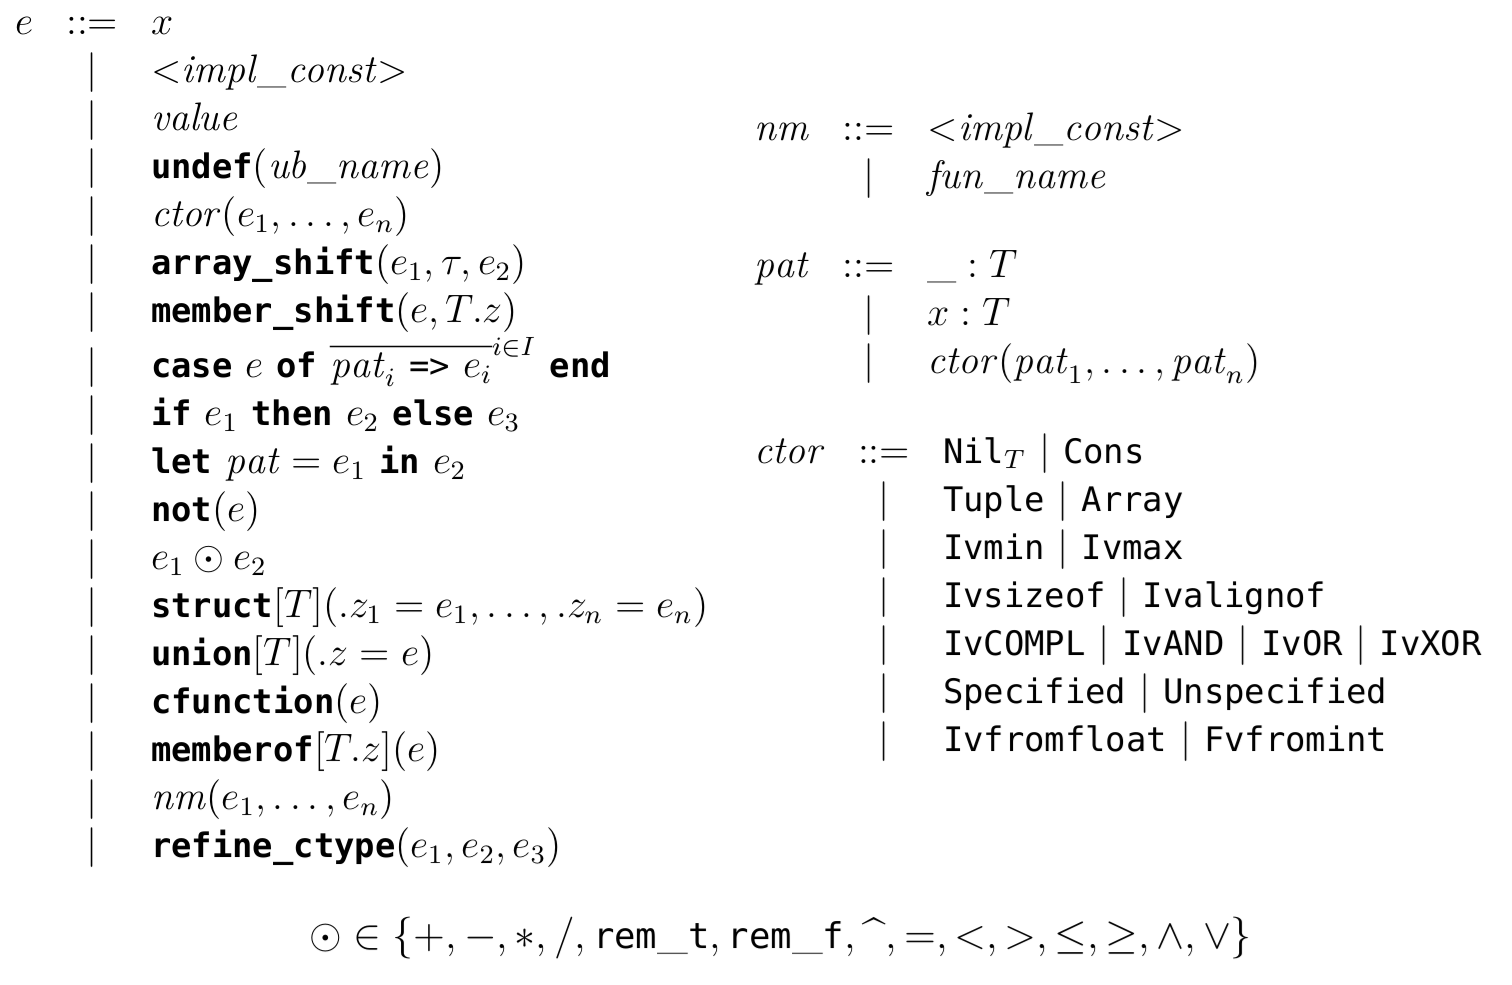
\includegraphics{figures/pure-core.png}
    \caption{The pure fragment of Core.}\label{fig:pure-core-grammar}
\end{figure*}

The effectful fragment captures interactions with memory (via a memory
interface), various ordering constraints, and more exotic control flow with a
goto-like operator used in the elaboration of C's iteration and \cinline{goto}
statements. The distinction between the pure and effectful fragments is is in
fact unrelated to the distinction between expressions and statements in C,
since both are elaborated into effectful expressions (for example,
\coreinline{PtrEq} which tests for for pointer equality).

I will discuss \coreinline{memop()} in more detail in % chktex 36
\nameref{chap:mem-model-explained}. For now it suffices to say that the
operations are effects, part of the memory interface \kl{Core} uses to abstract
over choices of different handlers, implementations of those effects in a
specific memory object model.

The following constructs are all related to evaluation order:
\coreinline{neg()}, \coreinline{unseq()}, \coreinline{let weak}, % chktex 36
\coreinline{let strong}, \coreinline{bound()}, \coreinline{nd()}, % chktex 36
\coreinline{par()}. These were supported in the implementation but  % chktex 36
stopped working due to a refactor of the resource inference scheme, and not
enough of a priority to re-enable. I did not attempt to formalise their
operational behaviour.\sidenote{The technique for doing so would simple
enough conceptually (using fractional-permissions), but capturing the allowable
behaviours in the type system accurately and threading it through the rest of
the formalisation would add unnecessary noise and complexity at this stage.}

The \coreinline{ccall()} and \coreinline{pcall()} constructs for calling % chktex 36
elaborate C functions and Core procedures (effectful functions) respectively.
They differ only in how the name of the procedure to be called is found, with
\coreinline{ccall()} using the memory interface to do so. % chktex 36

The \coreinline{save()} operator is \kl{Core}'s way of introducing named % chktex 36
continuations with default arguments. The label $l$ and arguments $x_1, \ldots,
x_n$ are in scope in $E$; those variables are associated pure expressions
provided by the \coreinline{run()} operator or with the default $e_1, \ldots, % chktex 36
e_n$ otherwise if the operator is reached otherwise. This is the \cinline{goto}-like
operator referred to earlier, which is used to elaborate all of C's iteration
and \cinline{goto} statements.

The important aspect from our purposes is that while control flows into
\coreinline{ccall()}, \coreinline{pcall()} and \coreinline{run()}, it % chktex 36
only returns from the first two and not the last.

\begin{figure*}[tp]
    \ContinuedFloat{}
    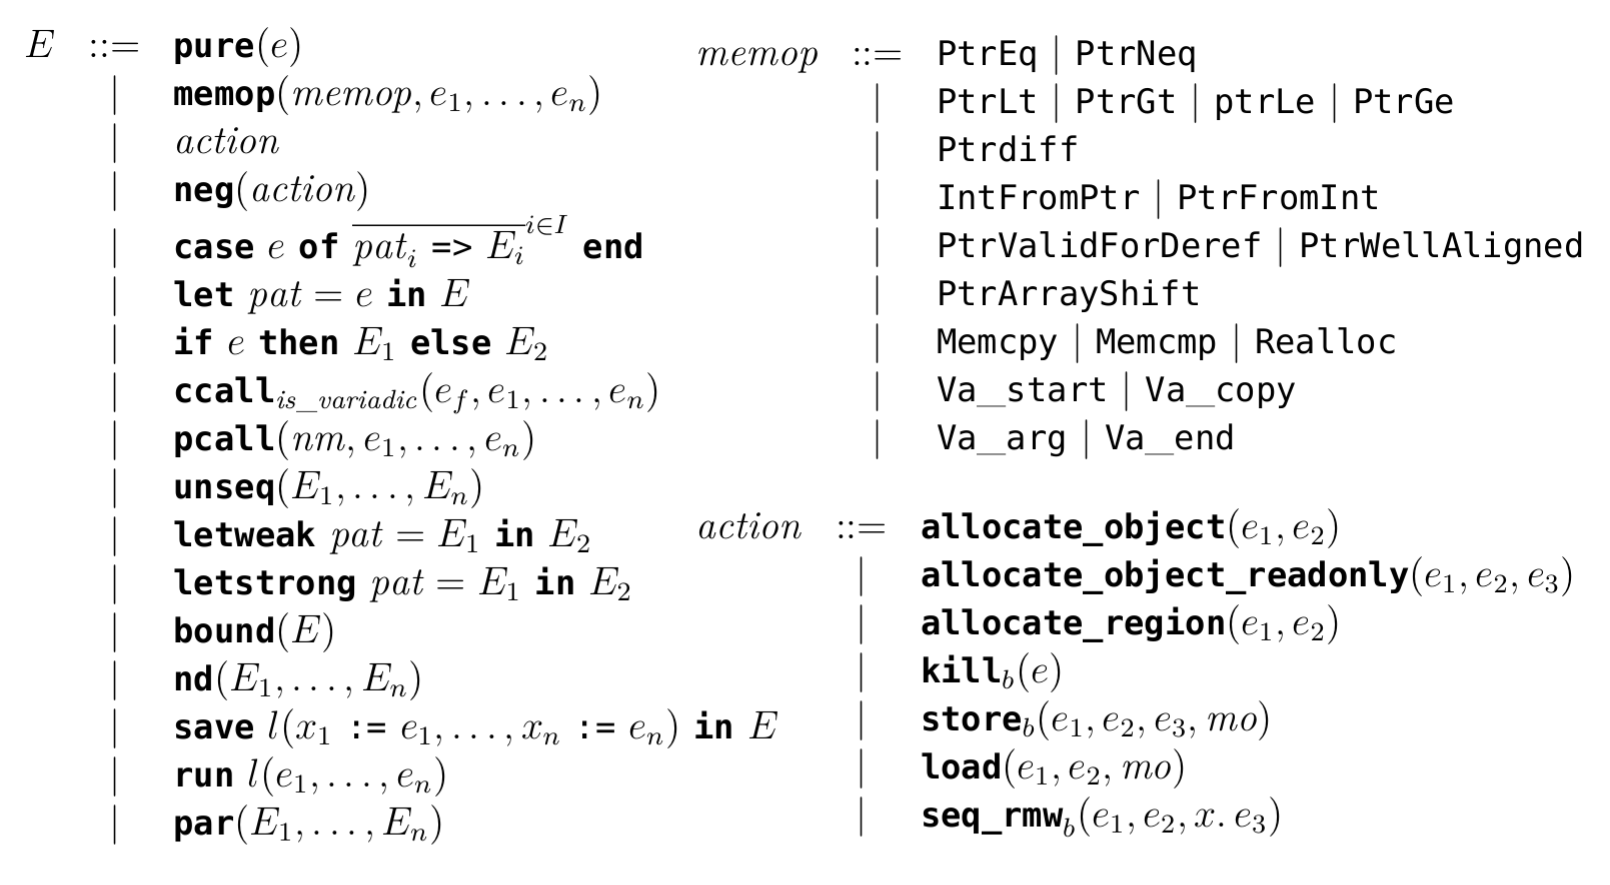
\includegraphics{figures/effectful-core.png}
    \caption{The effectful fragment of Core.}\label{fig:effectful-core-grammar}
\end{figure*}

We can see an example of Cerberus' elaboration into \kl{Core}, by recalling the
singly-linked integer list append function from \cref{fig:append-c}, reproduced
in \cref{fig:append-c-formal} for convenience.

\begin{marginfigure}
    \centering
    \cfile[breaklines]{code/append_plain.c}
    \caption{Singly-linked integer list append in C.}\label{fig:append-c-formal}
\end{marginfigure}%

\begin{figure*}[p]
    \centering
    \begin{minipage}{1.2\textwidth}
        \corefile{code/append_plain.core}
    \end{minipage}
    \caption{Elaboration of singly-linked int list append in C into
        \kl{Cerberus} \kl{Core}; library functions and \cinline{else}-branch
        omitted.}\label{fig:append-core}
\end{figure*}%

The elaboration is presented in \cref{fig:append-core}. To save space,
definitions the \kl{Core} standard library are omitted, as are choices about
implementation-defined details and the elaboration of the
\cinline{else}-branch. A few things are note-worthy:
\begin{itemize}
    \item The translation is \intro{compositional}. Each function, block,
        statement and expression is elaborated in isolation, based only
        on its parts, and follows the structure of the original C program.
    \item Each variable function argument and local gets its own storage via the
        \coreinline{create} function. Reads, writes, and de-allocations are
        represented with \coreinline{load}, \coreinline{store},
        \coreinline{kill} respectively.
    \item Loose evaluation order (for example between the expressions of a \cinline{==})
        are represented using \coreinline{unseq} and \coreinline{let weak} constructs.
    \item UB is made explicit in the syntax of the program, for example if \cinline{xs} was
        an unspecified pointer value (line 23) or if the function exited without a return statement
        and its `return value' was used elsewhere (line 71).
\end{itemize}

In particular, \kl{compositional}ity is just as important, if not more, than the
target language being a first-order functional language with effects. Given
that we want users to annotate programs at the C level, if we wish to type
check \kl{Core}, we need to be able to transport those annotations through the
elaboration process too, and place them at the appropriate program points.

If \kl{Cerberus} were to have elaborated into a dataflow graph instead of \kl{Core},
such transporting would be a major undertaking in itself. It might achievable
for function pre- and postconditions, but would become much more challenging
for loops, and \coreinline{goto} and even between specific statement as proof
hints to \kl{CN}. With a \kl{compositional} mapping, placing annotations
structurally, and relating annotations mentioning C variables to \kl{Core}
variables becomes feasible.

In principle, the compositional mapping also ensures that errors in \kl{Core}
elaboration can be related back to useful source locations in the original C
program. However, in practice, though \emph{compositional}ity does
\emph{enable} this, it requires a good amount of engineering effort to
accomplish (\cref{sec:error-msgs}). Another challenge is that though
elaboration simplifies greatly the checked language, it also increases the
distance between the checked and the typed language, which is felt acutely when
attempting to relate failures in SMT queries back to what users wrote,
particularly when those SMT are part of an inference procedure, rather checking
C source assertions (\cref{sec:counter-ex}).

\section{Refinement Types}

What are refinement types? Why do we care about decidability? It's a short hand
for usable, SMT, imperfect proxy for performance, to be discussed later.

You can layer over the existing system (from Kayvan's thesis), \textendash{}
rule for undef means (previously YOLO) to context has to be false. E\.g\. same if-then-else twice, so dead code.

Liquid types.

\section{Linearity}

\subsection{Friendly and convenient syntax}\label{sec:friendly-syntax}
Separation logic types, syntax and restrictions for it.

Explicit witness to having permissions, which are linearly typed (just ingredients).

\section{Alternatives and Related Work}

\chapter{Kernel CN:\ A Bidirectional, Separation Logic Refinement Type System for Core}%
\label{chap:kernel-cn}

This will be a lot of pages.
Explain \intro{bidirectional} (for quantifiers), linear resources, constraints.
Explain enough rules \textemdash{} typing, operations, especially the weird heaps.
And of course, type safety statement and its proof.

\subsection{Resource Terms, Quantifier Inference}

Linear terms in a refinement type system.

(Dep ML, L3, F star, Jhala, ATS)

Different and unusual compared to Iris style \textemdash{} separation proofs outside the program.

Proof term in one sense, but also factors out operations for resource manipulation.

\subsection{Heaps}


\subsection{Type Safety}


\chapter{Kernel CN:\ Grammar}%
\label{chap:kernel-grammar}

\kl{CN} and \kl{Kernel} CN have different grammars. This is because \kl{CN} is
intended to be used by C programmers, whereas \kl{Kernel} CN is more for type
theorists, and also to be more convenient to work with as a formalism. The
primary differences are (a) \kl{CN} is implemented over (a version of)
\kl{Core}, whereas the \kl{kernel} is defined over a let-normalised version of
\kl{Core} (b) \kl{CN}'s grammar of types is close to the surface syntax and so
each construct serves many purposes whereas the \kl{kernel}'s grammar of types
is more traditional and each construct only serves one purpose.

In this chapter I will present the relevant parts of \kl{CN}'s syntax of
predicate definitions and assertions, and the \kl{kernel}'s syntax of types and
relevant terms, with a particular focus on explicit resource terms.

\section{CN Syntax}%

\begin{figure*}[tp]
    \centering
    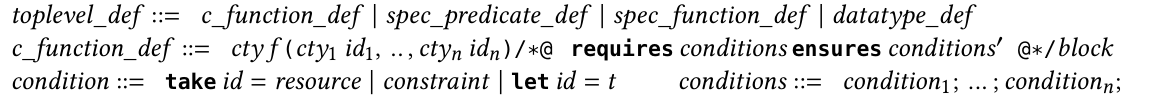
\includegraphics{figures/cn-grammar-1}
    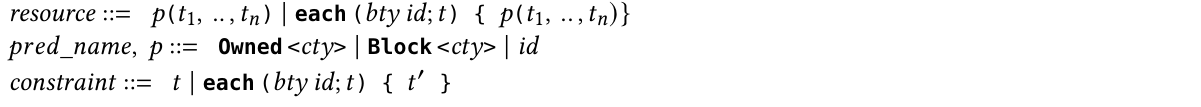
\includegraphics{figures/cn-grammar-2}
    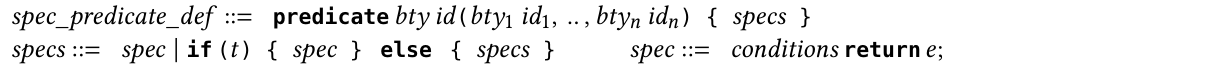
\includegraphics{figures/cn-grammar-3}
    \caption{Grammar of CN.}\label{fig:cn-grammar}
\end{figure*}

A file for \kl{CN} consists of series of top-level declarations of annotated C
functions, (separation logic) predicate definitions, (purely logical) function
definitions, and datatype declarations.\sidenote{Does the kernel formalism
support datatypes?} 

Function definitions for C introduce the identifiers for the arguments into the
scope of the pre- and postconditions, preceded by \cninline{requires} and
\cninline{ensures} respectively. Pre- and postconditions are a list of
`${conditions}$', each followed by a semi-colon.
\begin{itemize}
    \item \cninline{take id = resource} is a \kl{monadic} bind, which binds
        the \emph{output} arguments of the resource to the identifier \cninline{id},
        which doubles up as an assertion about the heap.
    \item \cninline{constraint} is a boolean-valued expression, which acts as a
        pure assertion.
    \item \cninline{let id = t} is simply an abbreviation for the expression
        \cninline{t} bound to \cninline{id}; it has no effect on the context.
\end{itemize}

\kl{CN} constraints (pure assertions) are either simple terms, or quantified
constraints.\sidenote{These must be manually instantiated by the user.}

\kl{CN} \kl{resource}s are simply a predicate \cninline{p(t1, .., tn)} % chktex 26 chktex 12 chktex 36
or an iterated predicate of the form
\cninline[breaklines]|each (<type> i; <guard>) { <pred>( array_shift(p i) ) }|. % chktex 36 chktex 37
Predicate names \cninline{p} are either
\cninline{Owned<ct>}/\cninline{Block<ct>}, representing ownership of an
initialised (read and write)/uninitialised location (a points-to $\mapsto{}$)
indexed by a C type, or \cninline{Alloc} representing an allocation, or a
user-defined one.

Similar to C syntax, \kl{CN} \kl{predicate} definitions first specify return
type, then a name, and a \intro{base type} annotated list of arguments. Their
definition consists of either a top-level \cninline{f} with a list of ${specs}$
in each branch, or a just the list of ${specs}$ at the top-level. ${specs}$ are
the ${conditions}$ followed by a return expression.

\section{Kernel CN types}

\begin{marginfigure}
    \centering
    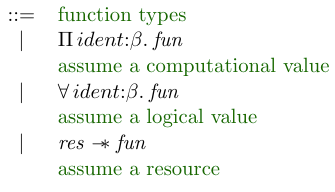
\includegraphics{figures/kernel-fun-1}
    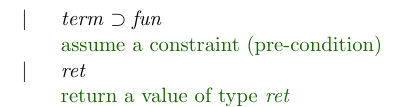
\includegraphics{figures/kernel-fun-2}
    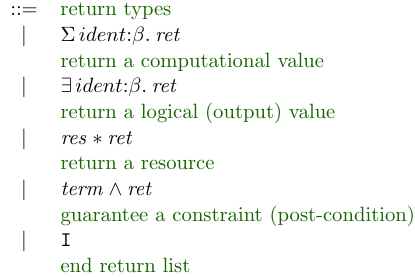
\includegraphics{figures/kernel-ret}
    \caption{\kl{Kernel CN} function and return types.}\label{fig:kernel-fun-ret}
\end{marginfigure}

\cref{fig:kernel-fun-ret} show the grammar of function types ${fun}$ which
include both pre- and postconditions, and return types ${ret}$, which
represents postconditions. Where the \kl{CN} grammar pre- and postconditions
are a flats list of ${conditions}$, these types are nested and have quantifiers
to make explicit their scoping, specifically that the variables bound in the
precondition are available for use in the postcondition. This is necessary
because these types depend on computational values, and so, for example, a call
to a function needs to propagate the symbolic or concrete function arguments
into the rest of a pre- and postcondition (via a spine judgement).

In order, both include: quantification over computational (program) values,
quantification over logical (ghost) values, separating implication/conjunction
for assertions about the heap,\sidenote{Should I change this (back) to
$\otimes$ and $\multimap$? Or would that be confusing?} and logical
implication/conjunction for pure assertions (in a linear context, about an
empty heap).

Though this seems like a large departure from the syntax given in
\cref{fig:cn-grammar}, the mapping into this is straightforward, and helps
clarify what each \kl{CN} surface construct represents in more familiar,
type theoretic terms.

Before I explain this mapping, there is one more key component left to explain:
\emph{resource types}. As seen in~\cref{fig:kernel-res}, they are type for
separation logic assertions, which will be treated linearly. The constructs are
quite standard, except for the only mention of branching in any of the types,
with the \emph{ordered} disjunction, to prevent the need for backtracking,
rather than the usual $\vee{}$.

For ease of implementation and formalisation, we do not have branching for pre-
and postconditions and function/return types, but this does not affect
expressiveness because these can be embedded into the resource types. Note that
in the formalisation, the branching is not restricted to the top-level in
predicate definitions, but can occur directly in function types, and can be
arbitrarily nested.

Predicates ${pred}$ and quantified predicates ${qpred}$ are simple
${pred\_term}$ and ${qpred\_term}$ with output arguments, as seen
in~\cref{fig:kernel-qpred}. I will explain why I factored out ${pred\_term}$
and ${qpred\_term}$ later. For now, I will draw attention to the fact that
where there is a distinction between \cninline{Owned} and \cninline{Block} in
the surface syntax, the formalisation tracks whether or not a points-to has
been initialised in a symbolic \emph{record} field ${.init}$, whose type
mirrors the structure of the C type, i.e.\ with leaves which are booleans, and
branches which are records or arrays. This allows for more fine-grained control
over reading and writing \emph{partially} (and completely) uninitialised reads
of structs/unions,\sidenote{\url{https://www.cl.cam.ac.uk/~pes20/cerberus/notes98-2018-04-21-uninit-v4.html\#reads-of-partially-uninitialised-structsunions-as-a-whole} % chktex 8
Though honestly I could just get rid of this because it would be simpler.} as
allowed by the C standard.

\begin{marginfigure}
    \centering
    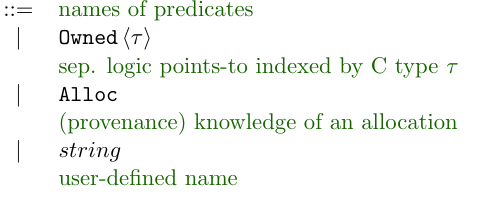
\includegraphics{figures/kernel-pred-name}
    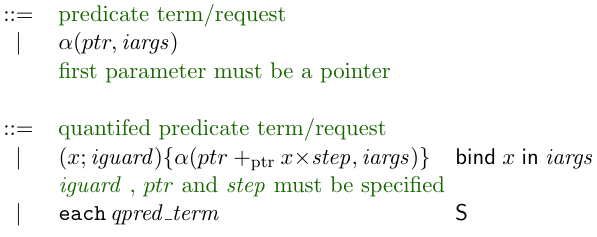
\includegraphics{figures/kernel-qpred-term}
    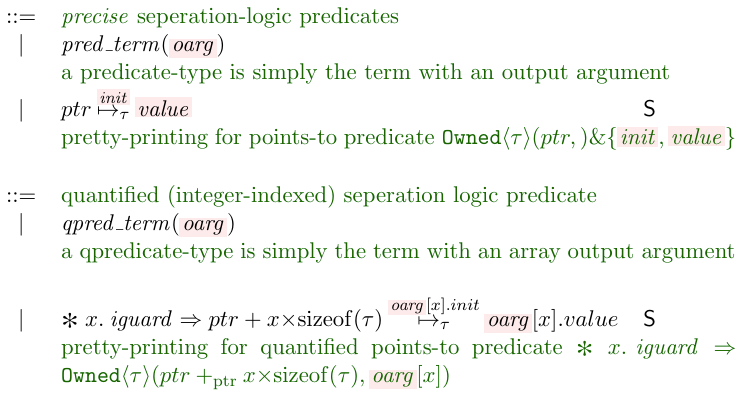
\includegraphics{figures/kernel-qpred}
    \caption{\kl{Kernel CN} predicate and quantified predicate terms (without
        output arguments) and types (with output arguments). The formalisation
        is set up with some syntactic sugar (marked with $\mathsf{S}$) to make
        the meanings of these constructs more intuitive.}\label{fig:kernel-qpred}

\end{marginfigure}

\begin{marginfigure}
    \centering
    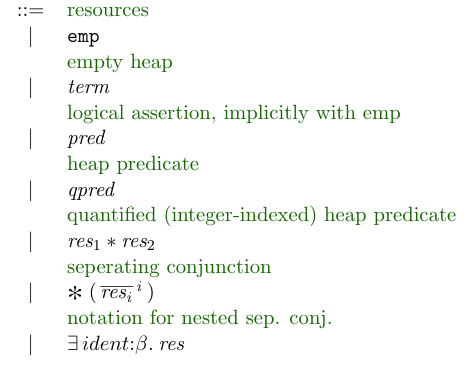
\includegraphics{figures/kernel-res-1}
    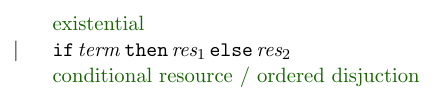
\includegraphics{figures/kernel-res-2}
    \caption{\kl{Kernel CN} resource types, a linear type for separation logic
        assertions.}\label{fig:kernel-res}
\end{marginfigure}

\section{Desugaring \kl{CN} types into \kl{kernel} types}\label{sec:desugaring}

All judgements in the formalisation which have a natural bidirectional
interpretation have the information they are synthesising highlighted with
\colorbox{pink!30}{light pink} background. The grammars presented below will
refer to ${term}$, ${iguard}$, ${ptr}$, ${init}$, ${value}$, ${iarg}$, ${oarg}$
(and later, ${alloc}$). These are all simply aliases for pure (SMT) terms, used
so that the roles of these terms in different productions, especially ones
productions which refer to multiple instances of them, are clearer. \intro{Base
types}, represented by $\beta$ or ${bty}$ are simply they types of such terms.

Desugaring \kl{CN} types into \kl{Kernel CN} starts with the C functions, which
map their parameters into computational variables in function types, or with
predicate definitions, which map their parameters into essentially a
$\lambda$-abstraction over a resource type (\cref{fig:prepost-to-kernel}). To
clear, this is merely quantifying over pure (SMT) terms in the type, rather
than any higher-order assertions about the shape of the heap.

\begin{figure*}[tp]
    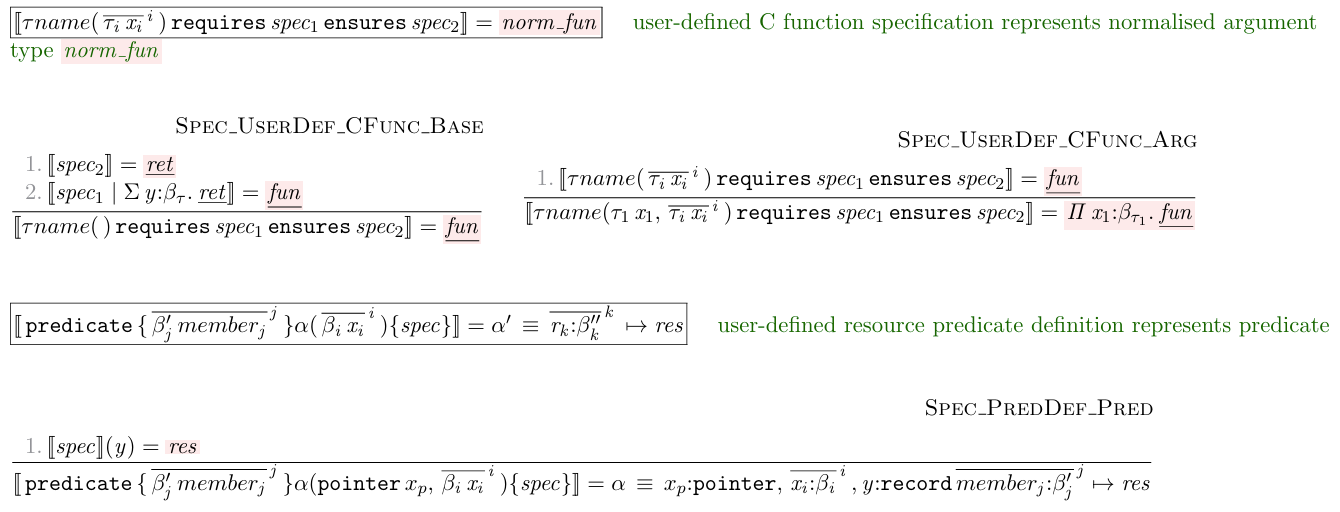
\includegraphics{figures/prepost-to-kernel}
    \caption{\kl{CN} to \kl{Kernel CN} pre- and postcondition and predicate
        definition desugaring. For the C functions, each C argument is bound to
        a computational argument, with a base type corresponding to the C type.
        Predicate definitions simply abstract pure (SMT) terms over
        resources.}\label{fig:prepost-to-kernel}
\end{figure*}

Desugaring preconditions into function types requires the postcondition to be
desugared first; because that is similar to precondition desugaring, I will
omit it for space. Abbreviations are simply substituted into the function
type.\sidenote{In the implementation, for better error messages, they are bound
to a fresh variable and constrained with an equality constraint.}\label{sn:abbrev}
Constraints are mapped into logical implications. The formalisation can handle
ifs directly in the precondition, unlike the surface syntax which allows ifs to be placed
only at the top-level of a predicate (\cref{sec:restriction-branching}).

The monadic binding \cninline{take id = ..} is always translated into a logical % chktex 26
quantification over the output argument of the (quantified)\sidenote{Should
really consider renaming these to `iterated predicates'.} predicates. Because
all the predicate definitions are guaranteed to be precise, all the logical
quantifications can be inferred when required.

\begin{figure*}[tp]
    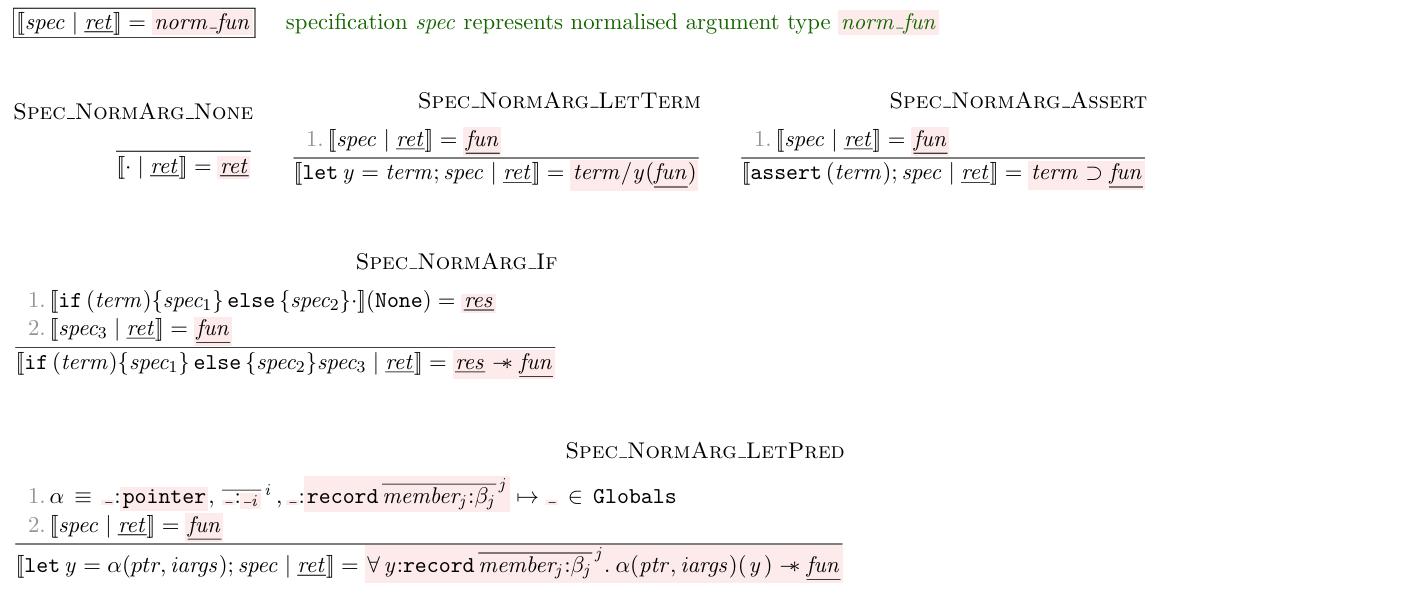
\includegraphics{figures/preconditions-to-kernel-1}
    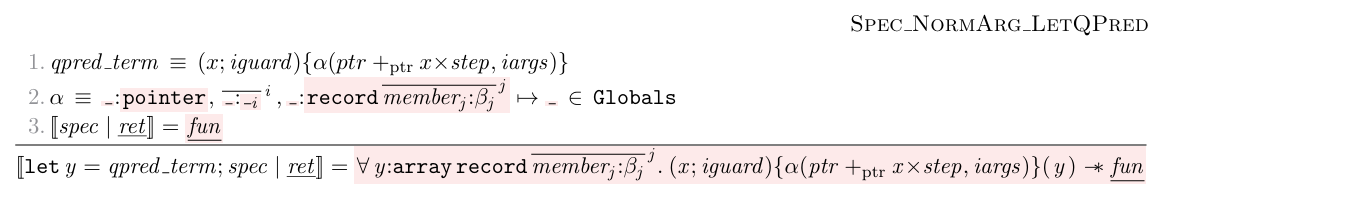
\includegraphics{figures/preconditions-to-kernel-2}
    \caption{\kl{CN} to \kl{Kernel CN} precondition desugaring.
        Postcondition desugaring is similar, and thus omitted.}\label{fig:precond-to-kernel}
\end{figure*}

Desugaring predicate definitions is similar. Because the grammar is used in two
contexts, inside a pre- or postcondition where a return is not allowed, and in
a predicate definition where a return is allowed, the desugaring is
parameterised over whether or not a return is expected. If one is not, then the
resource is simply an $\mathsf{emp}$, otherwise it is an equality constraint,
as shown in \cref{fig:monad-sl}. Outputs of (quantified) predicates are always
assumed to be of the shape of a record for uniformity, which I will justify
later. Abbreviation are also substituted in,\sidenote{As in note~\ref{sn:abbrev}.}
Because pure (SMT) terms are syntactically stratified out of
the impure ones, they are embeded directly into a resource type (separation
logic assertion) with $\astRef{}$. Ifs in the syntax are translated into ifs in
the resource type grammar, with some adjustment based on whether it occurs in a
terminal place; no returns are expected/allowed in non-terminal
ifs. This restriction side steps the need for a more complicated
destination-passing style \sidecite{shaikhha2017destination} transformation to
translate the semantics early-returns into precise separation logic
assertions. Lastly, as before, the monadic binding \cninline{take id = ..} is % chktex 26
always translated into a logical quantification over the output argument of the
(quantified) predicate.

\begin{figure*}[tp]
    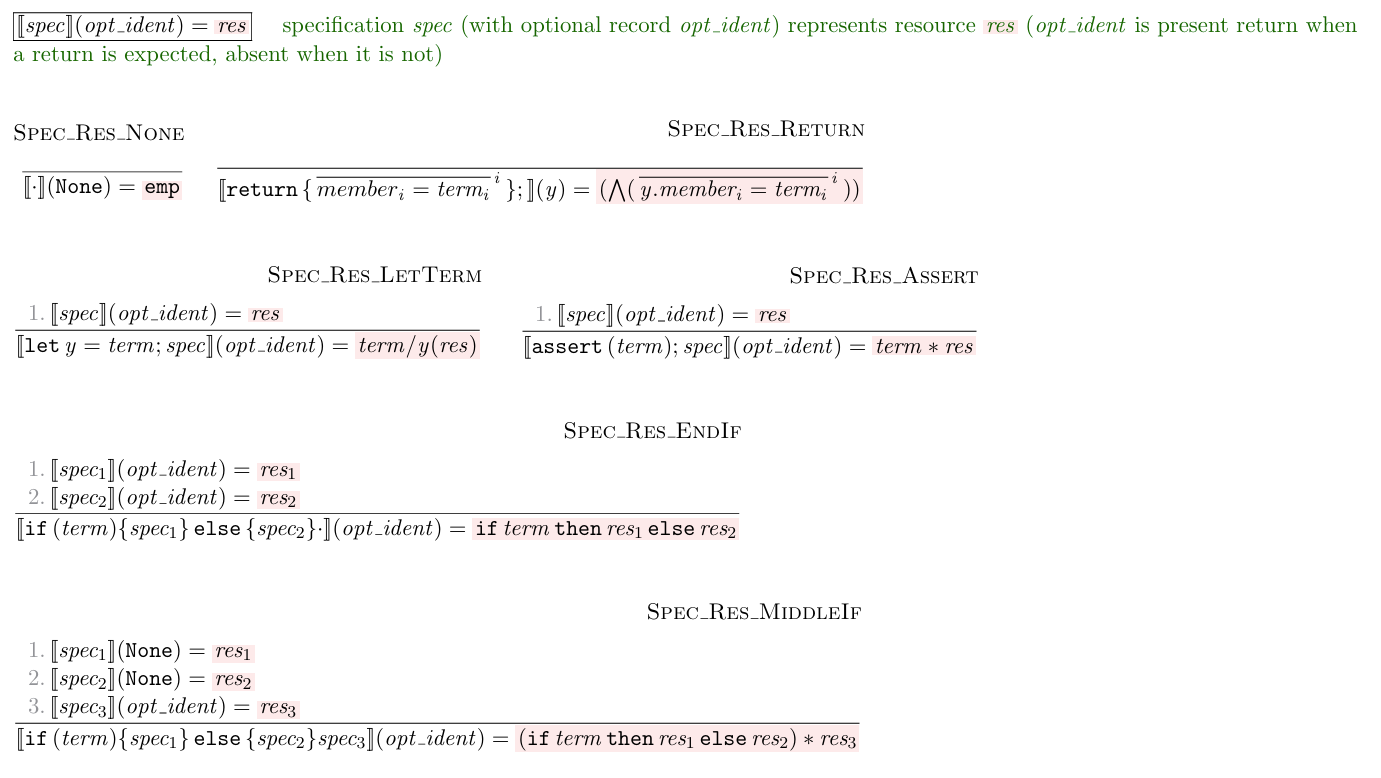
\includegraphics{figures/predicate-to-kernel-1}
    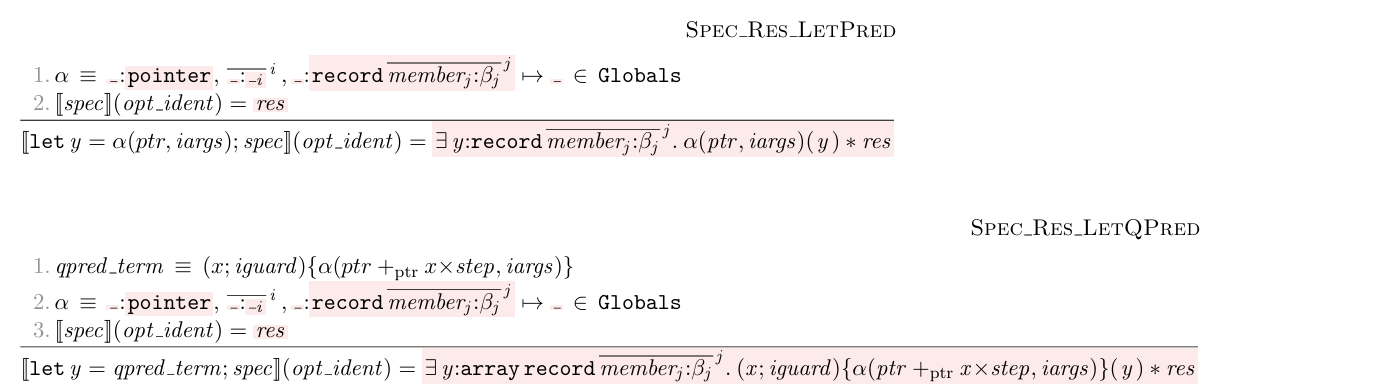
\includegraphics{figures/predicate-to-kernel-2}
    \caption{\kl{CN} to \kl{Kernel CN} user-defined predicate desugaring.}\label{fig:pred-to-kernel}
\end{figure*}

\section{Let-normal Core}

Not only is the formalisation defined over a desugar representation of types
from the surface \kl{CN} syntax, it is also defined over the let-normal form of
the \kl{Core} grammar
(\cref{fig:pure-core-grammar,fig:effectful-core-grammar}). By let-normal, I
mean an A-normal\sidecite{flanagan1993essence} form which is closed under
substitution.

Specifically, it syntactically stratifies values and
expressions from which we would like to \emph{synthesise} type information, and
top-level values and expressions against which we would like to \emph{check} a
given type. This applies to both pure and effectful fragments, leading to a
four-fold distinction in the let-normal form of the grammar.

This dramatically simplifies presenting and working with the type system, because:
\begin{itemize}
    \item \coreinline{undef()}. In typing this, it is necessary to give is a % chktex 36
        checking rule, since control flow is required to not reach that point
        (\cref:fig:core-ub-typing).
    \item \textbf{Control flow}. Here too, we would also very much like to use
        a checking rule, since this would alleviate the need to construct
        \emph{join}-points in types (or require users to place annotations
        after all \cinline{if}-statements).
    \item \textbf{Lets}. In typing these, we would also very much like to use a
        \emph{synthesis} rule for the bound expression, since that removes the
        need for an annotation to be placed on the binder there.
    \item \textbf{Memory actions}. These too are well-suited to synthesis, since
        they can manipulate they manipulate the resource context via the
        resources types they will synthesise.
\end{itemize}

Initial versions of \kl{CN} did a full A-normalisation of Core, but this resulted
in far logical variables being created (one for each intermediate sub-expression)
and these were very difficult to relate back to the source program in concrete
counter-examples produced by the SMT solver.\sidenote{Location information was not
tracked properly either so this was doomed.} Hence, this was
removed.\sidenote{\href{https://github.com/rems-project/cerberus/commit/21808139bda2ee320756c71eb22dbd57d0986f97}{Commit 21808139.}}.
The way that \kl{CN} currently manages the flow of information is by explicitly
passing around continuations; when it comes across any expression which is
treated as a top-level one in \kl{let-normal Core}, it simply does the appropriate
checks and then \emph{drops} the continuation.\sidenote{\href{https://github.com/rems-project/cerberus/commit/350fefc675626dcc69c7adc9edea30ff9687b752}{Commit 350fefc6.}}
This makes the code more fragile but saves the need for maintaining another large
syntax tree which needs pretty-printers, debug printers, source location
mappings and so on.

Since it would require more complex fractional permissions, I left out
let-normalising \coreinline{unseq()}, \coreinline{let weak} and other % chktex 36
constructs related to C's loose evaluation order. However, this also means
the formalisation glosses over the fact that those constructs can contain each
other in a semantically meaningful way, such that flattening out that nesting
seems impossible. The solution would be to require type-annotations on any
situation which requires top-level expressions to be nested inside one another.
Indeed, as we shall see in \nameref{chap:kernel-soundness}, annotations on
nested top-level expressions are required anyway for proving type preservation
for function calls to pure Core functions, effectful Core procedures, and
elaborated C functions. And as I demonstrate in \nameref{chap:kernel-alternative},
it seems very difficult to avoid some sort of normalisation somewhere in
the type system in the presence of early returns in sub-expressions.

For now, I will confine my discussion of the let-normal grammar to top-level
expressions (full details for both nested and top-level expressions are
available in the appendix). Pure expressions include things such as pure values,
datatype values, pointer arithmetic for arrays (in \kl{de facto}, not \kl{ISO})
and struct/union members, boolean negation, binary operations and relations, function
calls and assertions. Top-level values and expressions are in
\cref{fig:kernel-tp}. As mentioned earlier, constructs where control flow
should not reach, such as \coreinline{undef()} must be in a checking % chktex 36
judgement, so top-level values consists of them and regular pure values lifted
to the top.

\begin{marginfigure}
    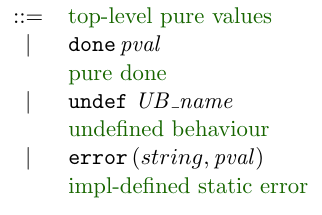
\includegraphics{figures/kernel-tpval}
    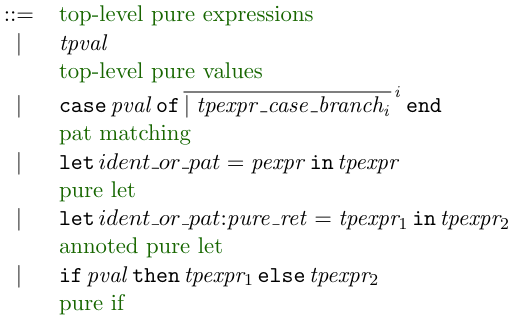
\includegraphics{figures/kernel-tpexpr}
    \caption{Top-level pure values and expressions in let-normal Core.}\label{fig:kernel-tp}
\end{marginfigure}

Top-level effectful values are the same as top-level pure values.
Effectful values and expressions are further split into \intro{sequenced}
expressions and \intro{indeterminately} sequenced expressions. Sequenced
expression include only C function calls and Core procedure calls.
As shown in \cref{fig:kernel-is-expr}, \kl{indeterminately} sequenced
expressions include annotated top-level values, memory operations, and explicit
terms to pack or unpack predicates (I will explain explicit resource terms in
\cref{subsec:res-terms}).

\begin{marginfigure}
    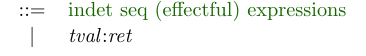
\includegraphics{figures/kernel-is-expr-1}
    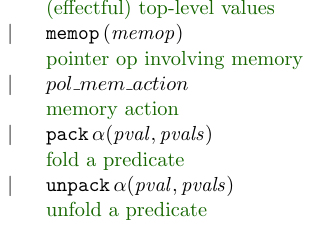
\includegraphics{figures/kernel-is-expr-2}
    \caption{\kl{Indeterminately} sequenced expressions in let-normal
        Core.}\label{fig:kernel-is-expr}
\end{marginfigure}


Sequenced top-level effectful expressions (\cref{fig:kernel-texpr}) are
simply the constructs which mention a pure expression inside them; you can see
that the bound expression in a \coreinline{let}, the scrutinee of a
\coreinline{case}, the condition of an \coreinline{if}, as well as the
arguments to \coreinline{run} are contain pure expressions
(\cref{fig:effectful-core-grammar}).

However, this are mutually defined with \kl{indeterminately} sequenced
top-level expressions (\coreinline{let weak} and \coreinline{let strong}), for
which as I mentioned before, I do not have accurate support. This is mutual
recursion is achieved the $\mathit{texpr}$ production.

\begin{marginfigure}
    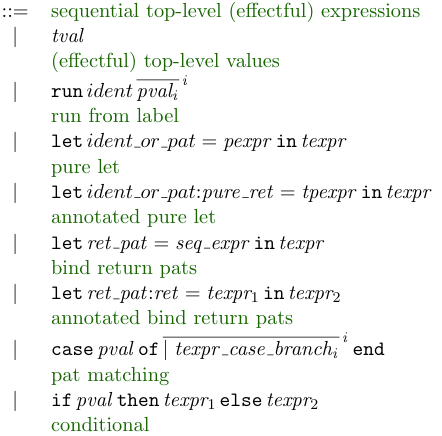
\includegraphics{figures/kernel-seq-texpr}
    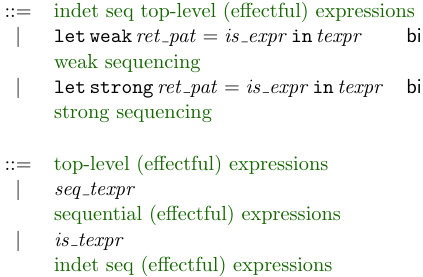
\includegraphics{figures/kernel-texpr}
    \caption{Top-level expressions in let-normal Core.}\label{fig:kernel-texpr}
\end{marginfigure}

\subsection{Resource terms}\label{subsec:res-terms}

\subsection{Heap types}\label{subsec:heap-types}

\subsection{Resource Terms, Quantifier Inference}\label{subsec:resq-inf}

Explain \intro{bidirectional} (for quantifiers), linear resources, constraints.
Explicit witness to having permissions, which are linearly typed (just ingredients).
Explain enough rules \textemdash{} typing, operations, especially the weird heaps.
And of course, type safety statement and its proof.
Linear terms in a refinement type system.

(Dep ML, L3, F star, Jhala, ATS)

Different and unusual compared to Iris style \textemdash{} separation proofs outside the program.

Proof term in one sense, but also factors out operations for resource manipulation.

\subsection{Heaps}


\subsection{Type Safety}

\chapter{Kernel CN:\ Typing rules}%

\chapter{Kernel CN:\ Proof of soundness}%
\label{chap:kernel-soundness}

Weird heaps.

\chapter{Informing implementation discussions}%

In the early stages, \kl{CN} was implemented by Christopher Pulte and Thomas
Sewell, based on sketches by Neel Krishnaswami. I started formalising
\kl{Kernel CN} much later, and benefited by the clarity of having an
implementations and implementers which and whom I could refer to in moments of
confusion.

However, this mode of development means that there were \emph{many} design
decisions made in a rather conservative context, because the programming was
always of a system which was being defined along the way, rather than a
well-understood pre-existing one. Extensions to syntax and inference were
always the minimum required for verifying the pKVM buddy allocator, lest
performance and inference suffer greatly, rather than ones based on a strong
formal and holistic consideration of the constructs and interactions at play.

As such, there are several restrictions in the implementation, which with the
benefit of hindsight and formalism, are completely unnecessary, but persist as
technical debt. This chapter list a few of these, and explains how the
formalisation brings much needed clarity to many questions around the
implementation.

\url{https://github.com/rems-project/cerberus/labels/language}
\url{https://github.com/rems-project/cerberus/labels/resource\%20reasoning}

\section{Supporting partially initialised reads of structs/unions}

This is not asked for, and actually seems to add a non-trivial amount of noise
and book-keeping to the formalisation. This suggests that the feature is not
worth implementing in CN unless a strong use-case comes up.

\section{Auto unfolding scheme for logical functions}
\url{https://github.com/rems-project/cerberus/issues/483}

\section{Higher-order resources}
\url{https://github.com/rems-project/cerberus/issues/483}

\section{Restrictions on branching}\label{sec:restriction-branching}
\url{https://github.com/rems-project/cerberus/issues/483}
\url{https://github.com/rems-project/cerberus/issues/266}

\section{Removing the pointer first restriction on predicates}
\url{https://github.com/rems-project/cerberus/issues/303}

\section{Unifying the syntax of functions, predicates and specifications}
\url{https://github.com/rems-project/cerberus/issues/304}


\chapter{An alternative presentation}\label{chap:kernel-alternative}

Perhaps a short chapter about MiniCN\@? This could demonstrate the strong
advantages of defining a type system over a first-order functional language,
rather than trying to do so directly over something C-like.

It would also give some space to the interesting but yet-to-be-baked ideas
from the Fuliminate paper.


\chapter{Kernel CN:\ Static semantics}\label{chap:kernel-statics}

\margintoc{}%
%
I have covered a large amount of background to the type system so far:
\intro{Core}, liquid types, bidirectional type systems, linear types, precise
separation logic assertions, monadic syntax for the latter and its relation to
kernel syntax for types, let-normalisation and explicit resource terms in
\kl{ResCore}. I use all of these ingredients in defining the type system for
\kl{kernel CN} that I will explain in this chapter. Some of the sections will
based on my contributions to~\sidetextcite[4.5cm]{pulte2023cn}%

The \kl{Kernel CN} type system is ordinary \kl{CN}, defined over \kl{ResCore}
instead of \kl{Core}, without any type or resource inference. In particular, It
requires that that all universal quantifiers are explicitly instantiated, that
all existential quantifiers have explicit witnesses, and all resource
operations are embedded into the program itself as linearly typed proof terms.
It does not require proof terms for the logical properties, since by
construction all of the entailments fall into the decidable SMT fragment; many
rules rely on this. The lack of inference make it a simpler language for which
to prove type soundness, whilst still demonstrating all the key ingredients
mentioned above. Since it handles the majority of C, the entire system is very
large, and so I will only discuss the main features.

There are some additional minor differences between the implementation and the
formalisation. As I mentioned \nameref{sec:desugaring}, the formalisation has a
richer grammar of resources: this makes defining predicates to represent tagged
unions more succinct, and allows for opening predicates in more cases. The
formalisation assumes that iterated resources output arguments have type array
of records, whereas the implementation uses records of arrays.\sidenote{This
purely a notational convenience so I could avoid inventing syntax for indexing
over an arbitrary record of arrays.}

Along with the type system, I briefly discuss a formalisation of two different
elaboration algorithms: one for inferring instantiations of logical quantifiers,
one for inferring indices for \kl{iterated} predicates. Because of a change
to the inference scheme used by \kl{CN}, the latter algorithm is no longer
used.\sidenote{\href{https://github.com/rems-project/cerberus/commit/7c2c0a364a4373e4eb109f32d01cc9584f51e81f}{Commit
7c2c0a36.}}\label{sn:new-inf-statics}

\section{Contexts}

The contexts for the static semantics consist of four parts: (1) $\mathcal{C}$
containing the computational variables from the Core program; (2) $\mathcal{L}$
containing purely logical variables mentioned in specifications; (3) $\Phi$,
the constraint context, containing a list of (non-quantified) SMT constraints;
and (4) $\mathcal{R}$ a \emph{linear} context containing the resources
available at that point during type-checking. I assume a constraint context of
only non-quantified constraints because users are required to manually
instantiate quantified constraints to use them.

\section{Pure values and expressions}

\kl{ResCore} programs have both computational and logical (ghost) terms.
Every such term, computational or ghost, has a \kl{base type} $\beta$,
which are things like unit, booleans, (mathematical) integers,\sidenote{After the formalisation was completed,
\kl{CN} switched from using mathematical unbounded integers to bit vectors
(\href{https://github.com/rems-project/cerberus/commit/8fdd4198750446de3b44d00f9e8f185db9610fab}{around
commit 8fdd41987}) to better support common bit-twiddling idioms, used heavily
in the buddy allocator in pKVM, without resorting to lots of lemmas about
uninterpreted functions.} locations, and records and user-defined algebraic datatypes of
other base types. Each C type $\tau$ is mapped to a corresponding base type $\beta_\tau$
\textemdash{} for example, $\beta_{\mathtt{int*}} = \mathsf{loc}$.

Logical terms are variously referred to as ${term}$, ${iguard}$ (for boolean
index guards of iterated predicates), ${ptr}$ (for pointers), ${init}$ (for
initialisation status), ${value}$ (for pointees), ${iarg}$ (for input mode
arguments to predicates),  ${oarg}$ (for output arguments for type record or
array of records), and later, ${alloc}$ (for constraints about the allocation
history).

As seen in \cref{fig:typing-pval-pexpr}, the rules for pure
values\sidenote{Because \kl{Core} factors out the memory object model, it also
factors out the precise representation of memory objects such as integers,
pointers, arrays and structs, so I have followed a similar factorising in
the structure of the typing judgements, and left the representation of these
values abstract.} are very simple pure value synthesis judgements of the form
$\mathcal{C} \vdash \mathit{pval} \Rightarrow \colorbox{red!8}{\beta}$;
given computational context and a pure value, synthesise a base type.

Building on the rules for pure values, the pure expression synthesis judgements
are not that much more complicated either: $\mathcal{C}; \mathcal{L}; \Phi
\vdash \mathit{pexpr} \Rightarrow \outpol{pure\_ret}$. Given a computational
context, a logical context, a constraint context and a pure expression,
synthesise a \emph{pure} return type (a return type without any resources or
logical variables). The use of return types starts to introduce a few more of
the refinement type features gestured at earlier. The type $\Sigma y {:}
\beta.\ \phi(y) \wedge{} I$ is simply the usual refinement type $\{ \, y \in
\beta \mid\phi(y) \, \}$, translated over to the grammar of types in \kl{Kernel
CN}. Recall that $\Sigma$ is used to bind a computational value in a
\emph{return} type, so these types are simply expressing, symbolically, in
constraints, that these expressions will evaluate to a value. Pure values are
simply lifted into the grammar of SMT constraints with an equality constraint;
pure expressions are lifted similarly but with their equivalent symbolic
computation.

\begin{figure*}[tp]
    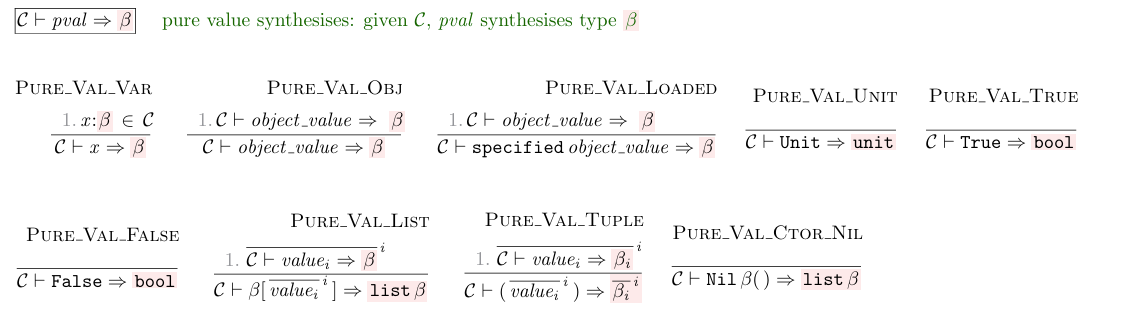
\includegraphics{figures/kernel-pval-typing}
    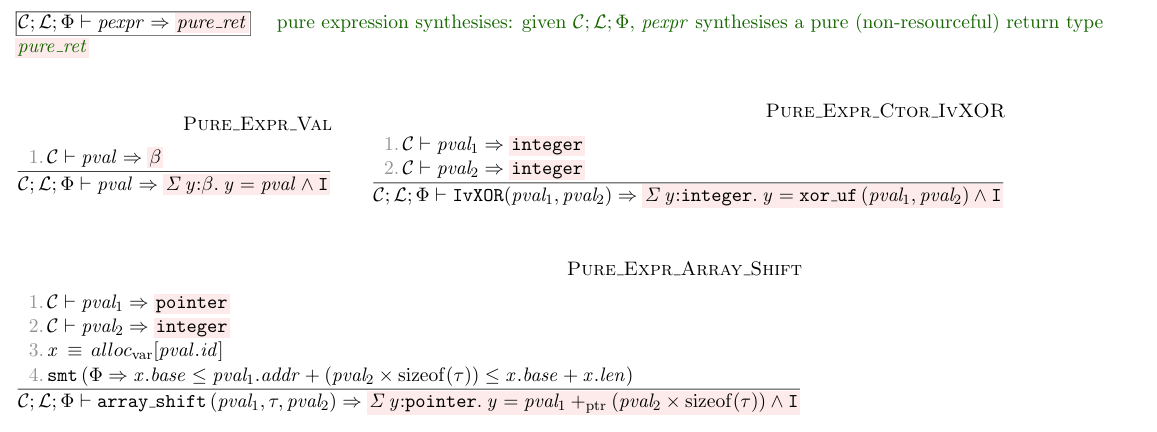
\includegraphics{figures/kernel-pexpr-typing}
    \caption{Selection of \kl{Kernel CN} typing rules for pure values and
        expressions.}\label{fig:typing-pval-pexpr}
\end{figure*}

\section{Top-level pure value values and expressions}

Whilst the rules for typing \emph{top-level} pure values and pure expressions
share the same context as typing pure values and expressions, they differ in
that they are \emph{checking} judgements instead of synthesising ones, of the
form $\mathcal{C}; \mathcal{L}; \Phi \vdash \mathit{tpexpr} \Leftarrow
\mathit{pure\_ret}$ (and similarly for $\mathit{tpexpr}$). Given the
computational, logical and constraint contexts, check the top-level value (or
expression) has satisfies this type.

Here we start to see the let-normalisation (\cref{sec:rescore}) and the
bidirectional (\cref{sec:bidir-subtyping}) approaches pay off. A top-level pure
value (i.e.\ the result of evaluating a pure expression) is checked against a
pure return type by checking if the constraint attached to it is true given the
context by calling the SMT solver, which is another reason why the constraints
being decidable is important and helpful. Similarly, the constructs we would
like to avoid (\coreinline{undef()} and \coreinline{error()}) check against % chktex 36
\emph{any} type, so long as the constraint context is inconsistent (can prove
$\mathsf{false}$). Top-level if-expressions synthesise a type for their condition,
but then check the branches, with an extra constraint on the true or false
value of the condition. Similarly, top-level let-expressions synthesise a type
for the bound expressions, and a constraint on the \emph{shape} bound value to
the context, and then check the body of the let.

The constraint on the shape of the bound value is produced by a judgement which
given a computational pattern (one inherited from Core) and a base type, it
produces a computational context and a term corresponding to the \emph{shape}
of the value according to the pattern match. For the sake of simplicity, I
assume all patterns are complete.

\begin{figure*}[tp]
    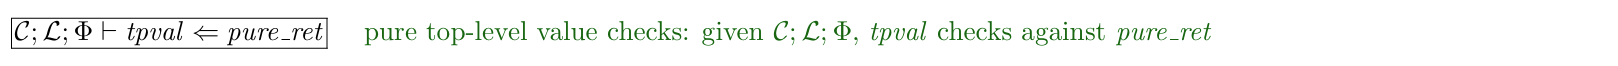
\includegraphics{figures/kernel-tpval-typing}
    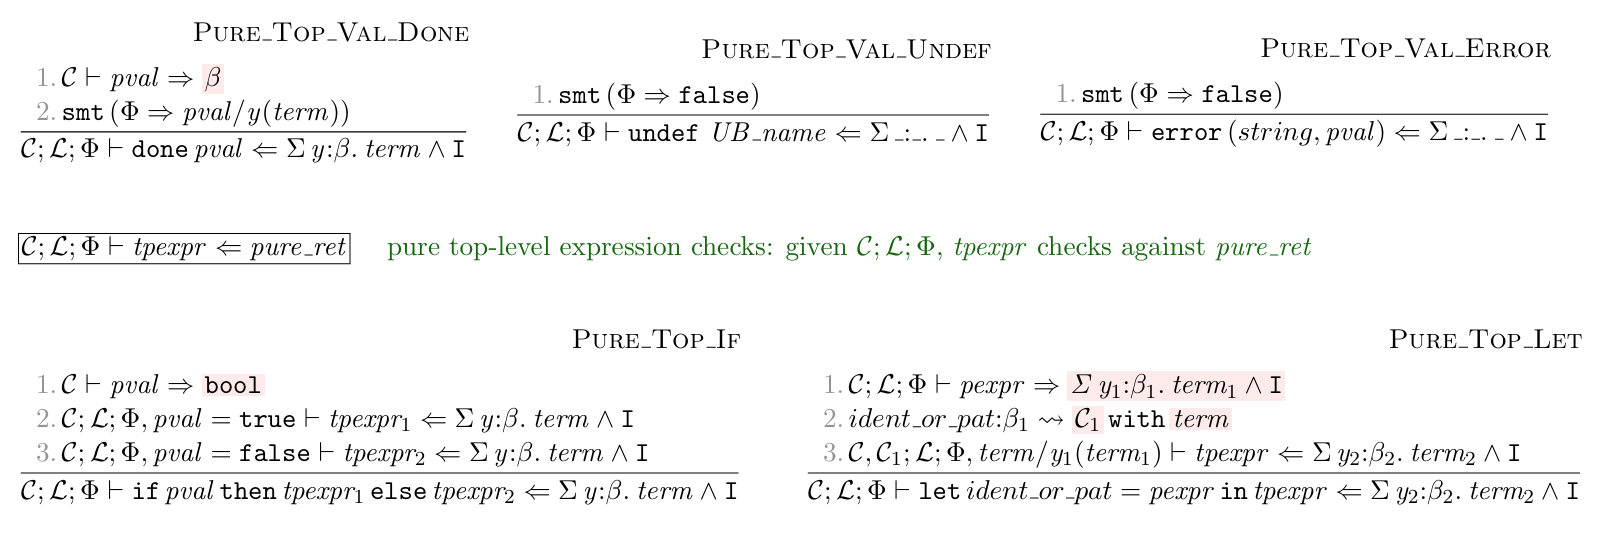
\includegraphics{figures/kernel-tpexpr-typing}
    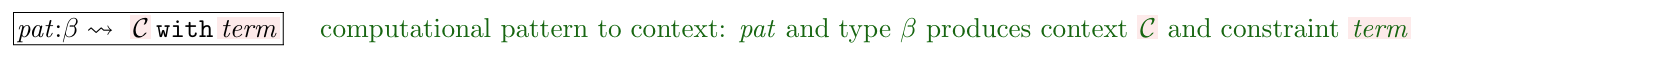
\includegraphics{figures/kernel-pat-comp-typing-1}
    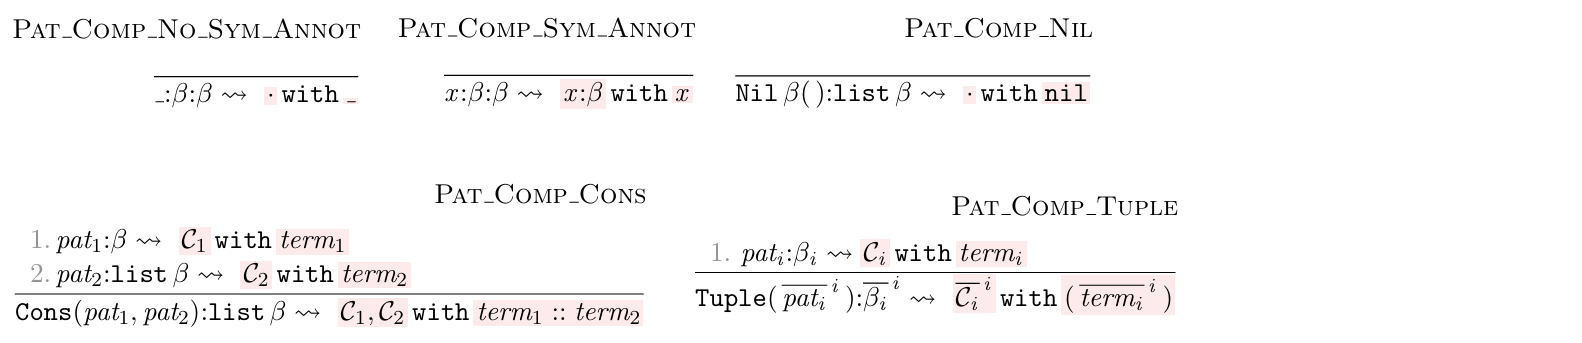
\includegraphics{figures/kernel-pat-comp-typing-2}
    \caption{Selection of \kl{Kernel CN} typing rules for top-level pure values and
        expressions, including the translation of computational patterns into a
        computational context used in the \coreinline{let} rule.}\label{fig:typing-tpval-tpexpr}
\end{figure*}

\section{Resource terms}\label{sec:typing-res-terms}

\begin{figure*}[tp]
    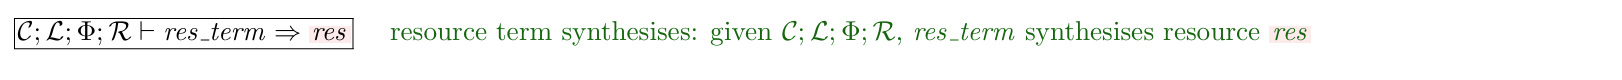
\includegraphics{figures/kernel-res-term-synth-1}
    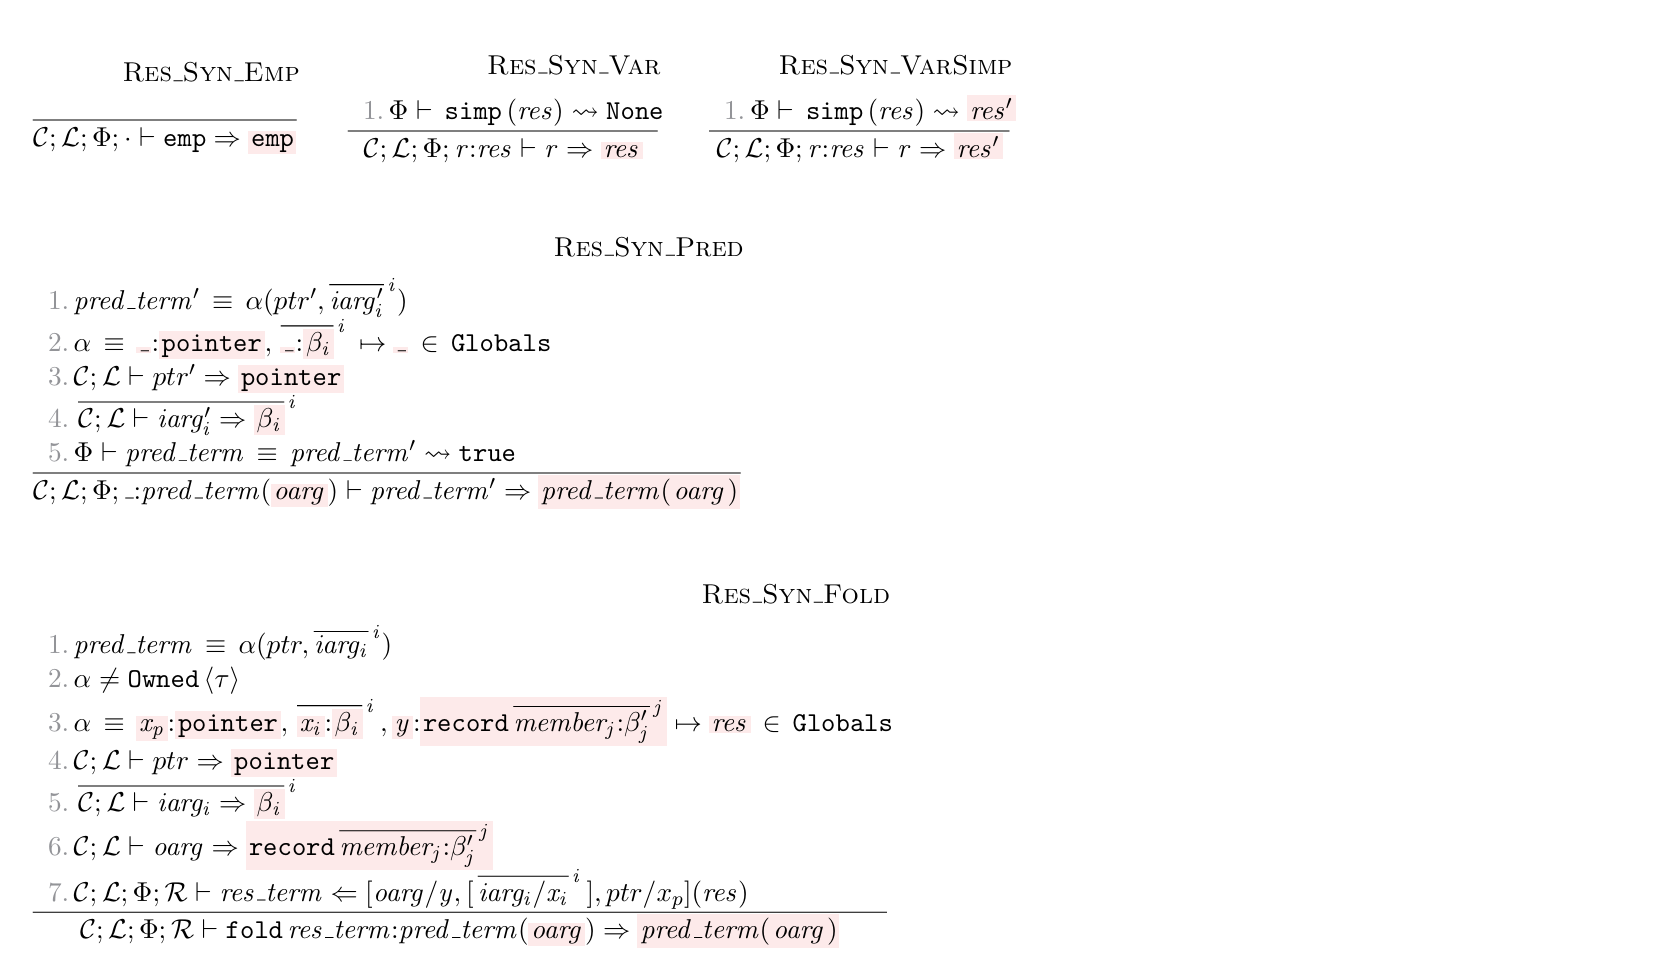
\includegraphics{figures/kernel-res-term-synth-2}
    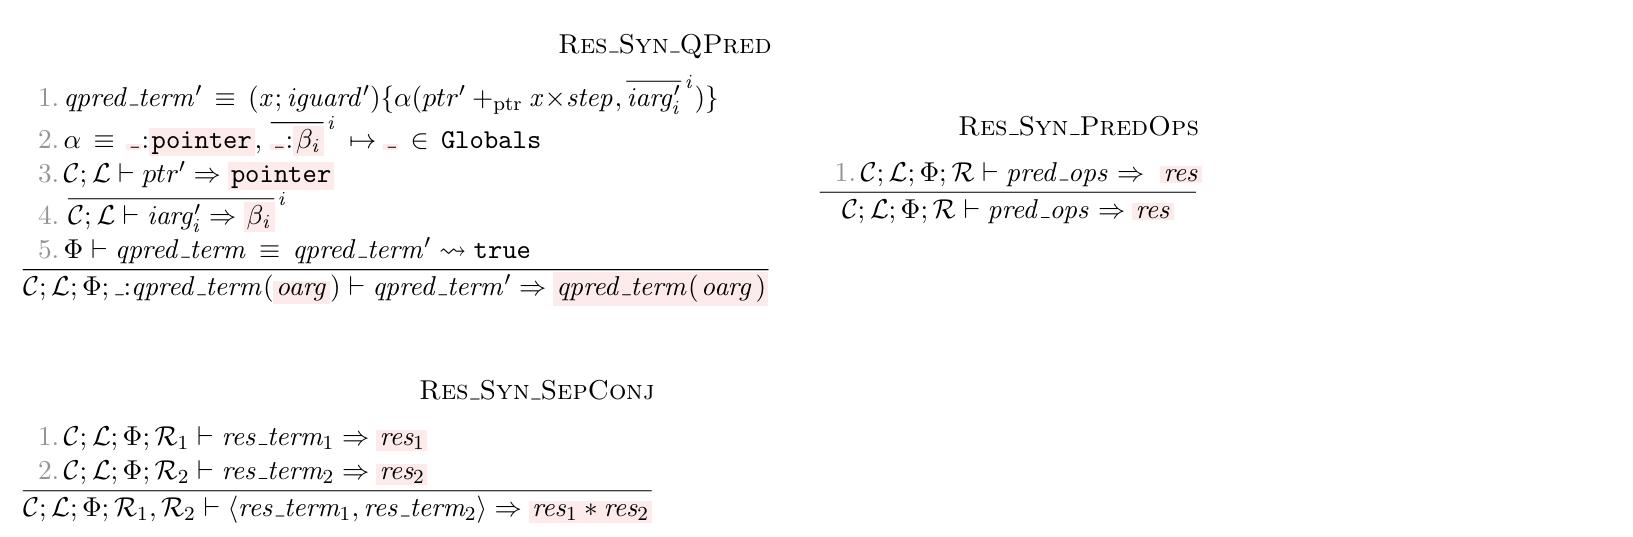
\includegraphics{figures/kernel-res-term-synth-3}
    \caption{Selection of \kl{Kernel CN} synthesising typing rules for resource
        terms.}\label{fig:typing-res-term-synth}
\end{figure*}

Typing resource terms requires the addition of an extra \emph{linear} context
$\mathcal{R}$ of resources. I will start with the synthesising judgements first,
and move on to checking judgements after.

\subsection{Synthesis for resource terms}\label{subsec:synth-res-term}

As visible in \cref{fig:typing-res-term-synth}, unsurprisingly, $\mathsf{emp}$
requires an empty context, and a variable use requires a singleton context.
Using variables also \emph{simplifies} them; simplification here just means
stripping as many top-level \coreinline{if}s off when their conditions are
provable to be true or provable to be false. Predicate (iterated and otherwise)
terms synthesise their types by checking the arguments (input and output) are
of the correct type. Note that (a) because of linearity, the context is a
singleton and (b) the lookup into the context is by predicate name $\alpha$ and
its input arguments, not by variable and (c) the output argument is synthesised
from the context. For ownership predicates, the input is the location, but the
output will be the initialisation status and the value stored at that location:
the program terms are not required to know what is in the heap.

Only user-defined predicates can be folded, so $\mathsf{Owned}\langle\_\rangle$
is excluded.\sidenote{Needs to be updated for $\mathsf{Alloc}$ too.} A term to
be folded is simply the (partially-evaluated) body of some predicate, so it
does not have the information required to know which predicate it could belong
to, especially because resources can and are moved between predicate. Hence,
morally, $\mathsf{fold}$ should be checked, not synthesised. However, in a
prior version of \kl{CN}, users were required to manually fold and unfold
predicates, and (by accident) that annotation was placed in an
indeterminately-sequenced expression, which also includes things like memory
actions. Memory actions are not well suited to be checked and are best
synthesised, and so this forced the fold/unfold annotations, and the resource
terms it contained, to also be synthesising.\sidenote{Of course, despite all
this, because the resource assertions are all assumed to be precise, we
could infer the output argument, but {Kernel CN} is meant to assume no
inference of instantiations to logical quantifiers, i.e.\ output arguments of
resources.} Hence, $\mathsf{fold}$ terms are annotated with the predicate which
they are meant to be folded into, so that the $\mathit{res\_term}$ it carries
can be \emph{checked} against the \emph{definition} (`body') of that predicate,
with the input and output arguments substituted in (after the arguments
are checked to be of the correct type).

\subsection{Synthesis for predicate operations}

Predicate operations are also synthesising and have their own judgement. And
because these operations can combine more than one kind of resource, they need
to synthesise separating conjunctions, so the rule for them is also
synthesising.

For space, I only present the rules for turning ownership of fixed size array
into an iterated separating conjunction and back (\cref{fig:typing-predops}).

The first rule says that if $\mathit{res\_term}$ synthesises ownership of a
fixed size array, then the iteration of that synthesises an iterated separating
conjunction for ownership over the indices of that array ($0$ to
$n-1$).\sidenote{The notational hacks in this rule are a bit too cute and
difficult to explain, should probably change them.} The second rule does the
inverse, but includes some additional checks to prevent two adjacent locations
of the same type but belonging to different allocations, being indexable from
a single base pointer.

\begin{figure*}[tp]
    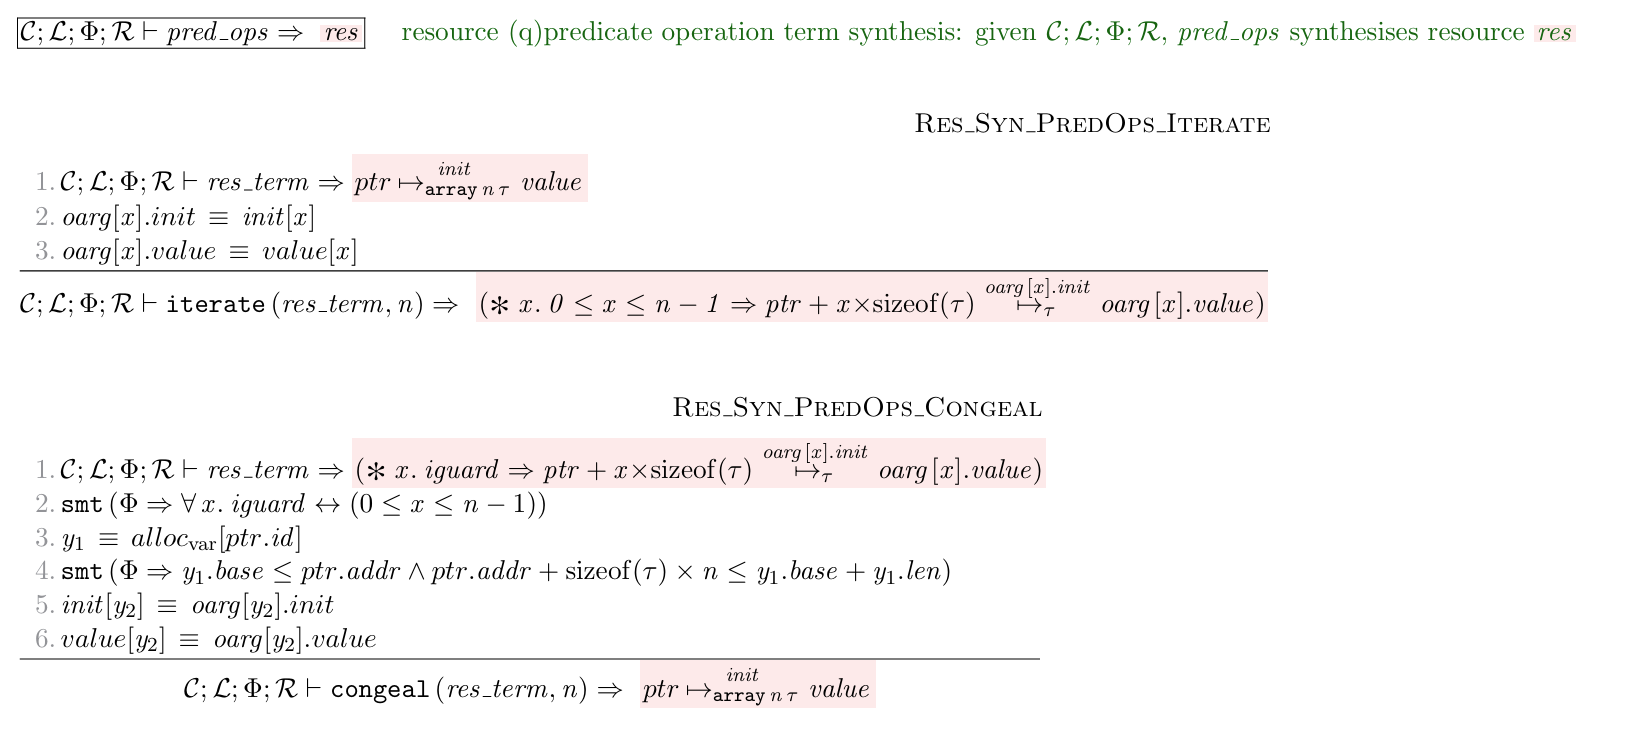
\includegraphics{figures/kernel-predops-typing}
    \caption{Selection of \kl{Kernel CN} synthesising typing rules for
        predicate operations.}\label{fig:typing-predops}
\end{figure*}

\subsection{Checking for resource terms}\label{subsec:checking-res-terms}

Lastly for the resource terms, we come to the checking rules. Resource terms
which represent constraints do not carry the constraint in them, and so need a
checking rule to learn them and prove them with a call to the SMT solver.
Similarly, because it is impossible to infer existential types in the general
case,\sidenote{Consider a heap $1 \mapsto 1$, and consider that all of $\exists
x.\ 1 \mapsto 1$, $\exists x.\ x \mapsto 1$, $\exists x.\ 1 \mapsto x$
(imprecise), $\exists x.\ x \mapsto x$ are valid inferences for it.} this too
is checking, and is straightforward since the instantiation is part of the
term, so it can be substituted into the type, which in turn can check the
$\mathit{res\_term}$ it carries.

As I mentioned earlier (\cref{sec:res-terms}), \emph{any} resource term can
introduce an ordered-disjunction, and so any resource term can be checked by
it. Furthermore, at most \emph{one} of the branches may be checked, and which
one depends on whether the condition or its negation can be proven. In the
situation that neither is possible, I call the condition (and the resource)
\intro{under-determined} (with respect to a constraint context). In this case,
the system may attempt to synthesise a type for the term and check that the
synthesised type is equal to the ordered-disjunction. Only variables can
synthesise an ordered-disjunction type, that too only if the condition is
under-determined (otherwise simplification will reduce it to either branch).
Separating conjunctions are also checked to allow for the case where an
existential or an ordered-disjunction are in the sub-components.

\begin{figure*}[tp]
    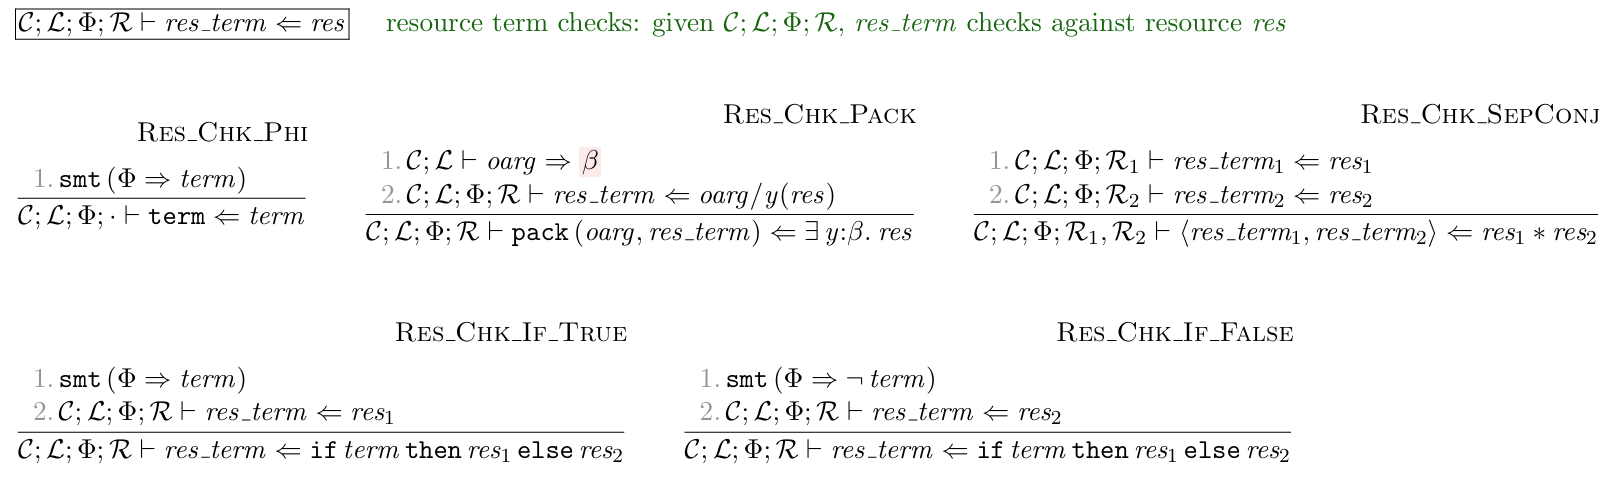
\includegraphics{figures/kernel-res-term-check}
    \caption{Selection of \kl{Kernel CN} checking typing rules for
        resource terms.}\label{fig:typing-res-term-check}
\end{figure*}

At any point, if the term cannot be checked by any other rule, the system can
switch to synthesising a type and then comparing whether the two types are
structurally equal, modulo SMT provability (\cref{fig:typing-res-term-check}).

\begin{marginfigure}
    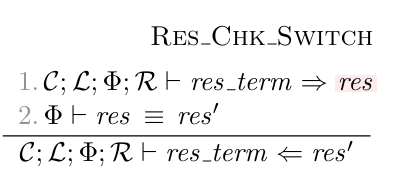
\includegraphics{figures/kernel-res-term-switch}
    \caption{Switching from checking to synthesising types for resource
        terms.}\label{fig:typing-res-term-switch}
\end{marginfigure}

\section{Memory actions and pointer operations}\label{sec:kernel-mem-action-ops}

As with resource terms, memory actions require all the contexts (computational,
logical, constraint and resource). The judgement $\mathcal{C} ; \mathcal{L} ;
\Phi ; \mathcal{R} \vdash \mathrm{mem\_action} \Rightarrow
\outpol{\mathrm{ret}}$ means that given the contexts and a memory action,
it synthesises a return type.

The rule for \coreinline{create()} is a bit busy because of % chktex 36
constraints on allocations required by the C standard (in premise 2), which I
will ignore. For now, the main thing to note is that the return type speaks of
the pointer to the newly created allocation as a computational value $y_p$,
constraints on pointer $y_p$ as required by the C standard, a unconstrained
logical (ghost) value for the pointee of the new allocation $x$, and the
finally the two resources it creates. The first is ownership of an
uninitialised piece of memory, at address $y_p$, and the second is an
allocation token $\mathsf{Alloc()}$ which is related to the memory object model
in \nameref{chap:cn-vip}.

In contrast, the rules for loads, stores and kill are quite simple. Loads
consume ownership of an initialised piece of memory\sidenote{For further
flexibility, loads of structs and unions could can be partially or completely
uninitialised, as allowed by the C standard, see
note~\ref{sn:partial-init-read}.}, check if the address of the load and the
address of the resource are symbolically equal, and synthesise a return type
mentioning the loaded value and ownership of the loaded location. Stores are
similar, but with extra checks on the stored value, which is also mentioned in
the ownership that is synthesised in the return type. Lastly, the rule for
\coreinline{kill()} is the converse of the one for \coreinline{create()}, % chktex 36
in that it \emph{consumes} the ownership and allocation token for a location
and synthesises a return type with no resources.\sidenote{I need to add the
rule for dynamic allocations.}

\begin{figure*}[tp]
    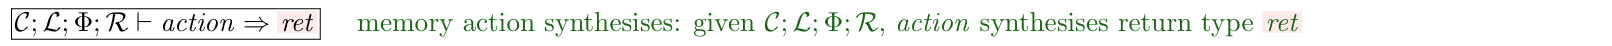
\includegraphics{figures/kernel-mem-action-typing-1}
    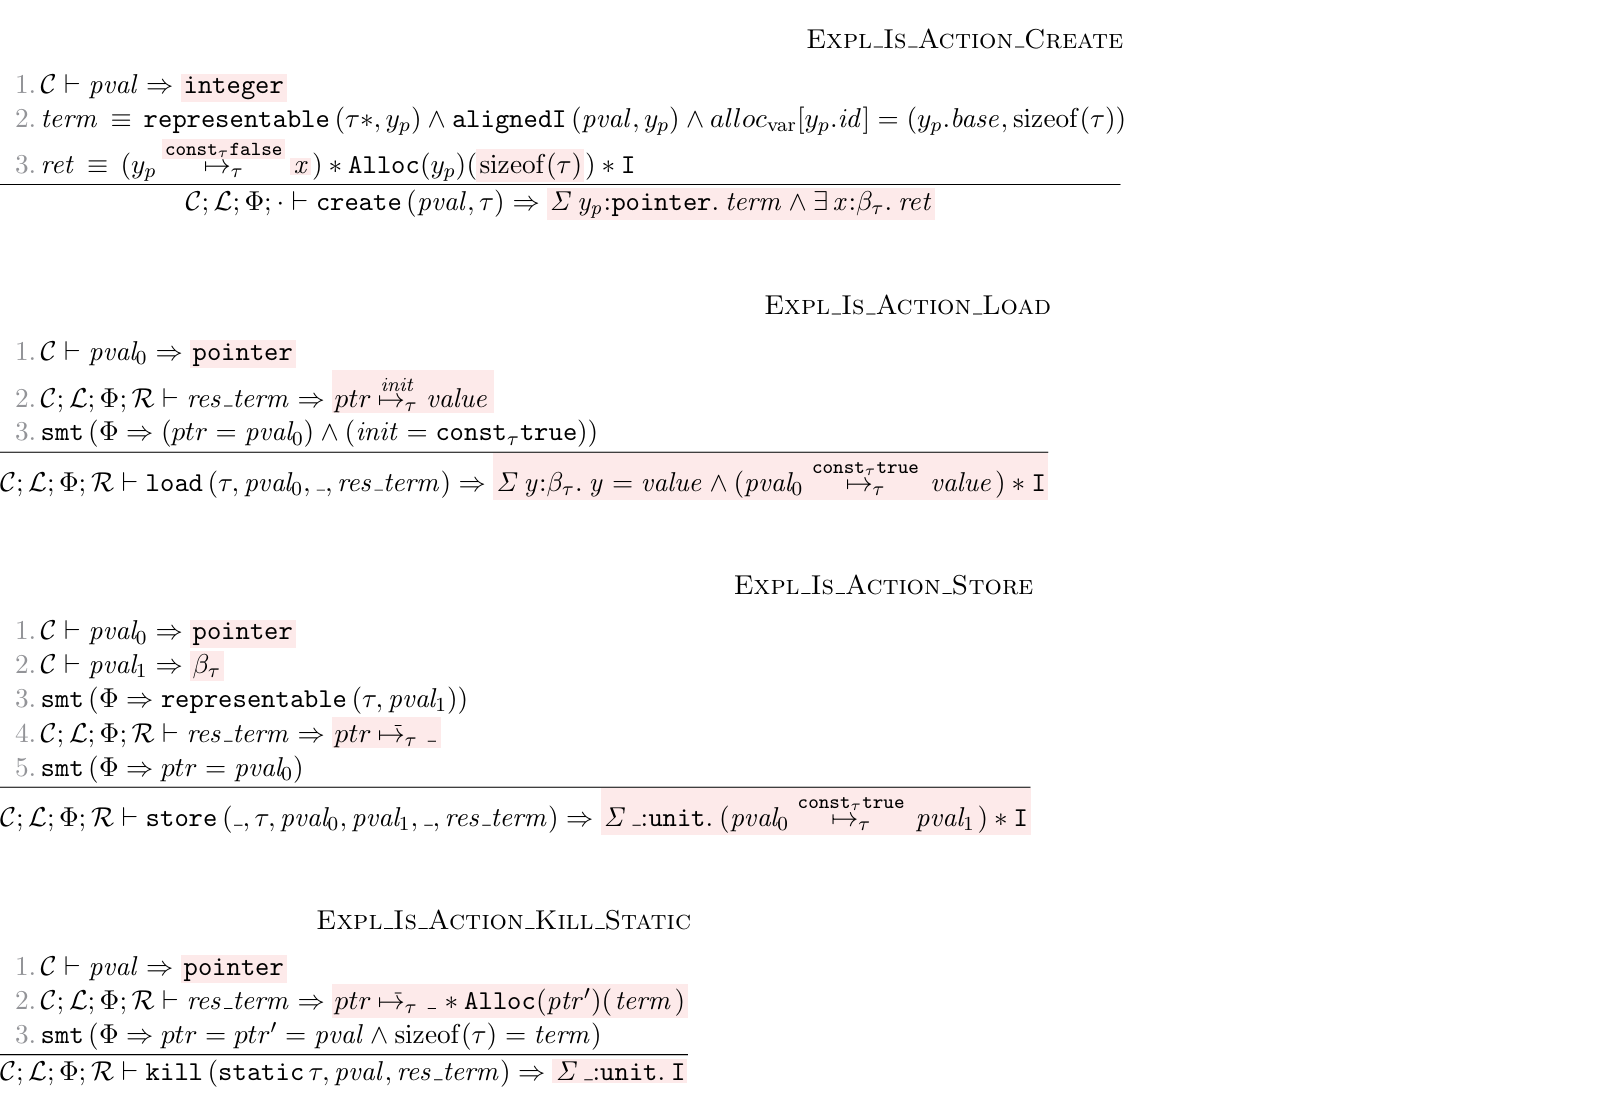
\includegraphics{figures/kernel-mem-action-typing-2}
    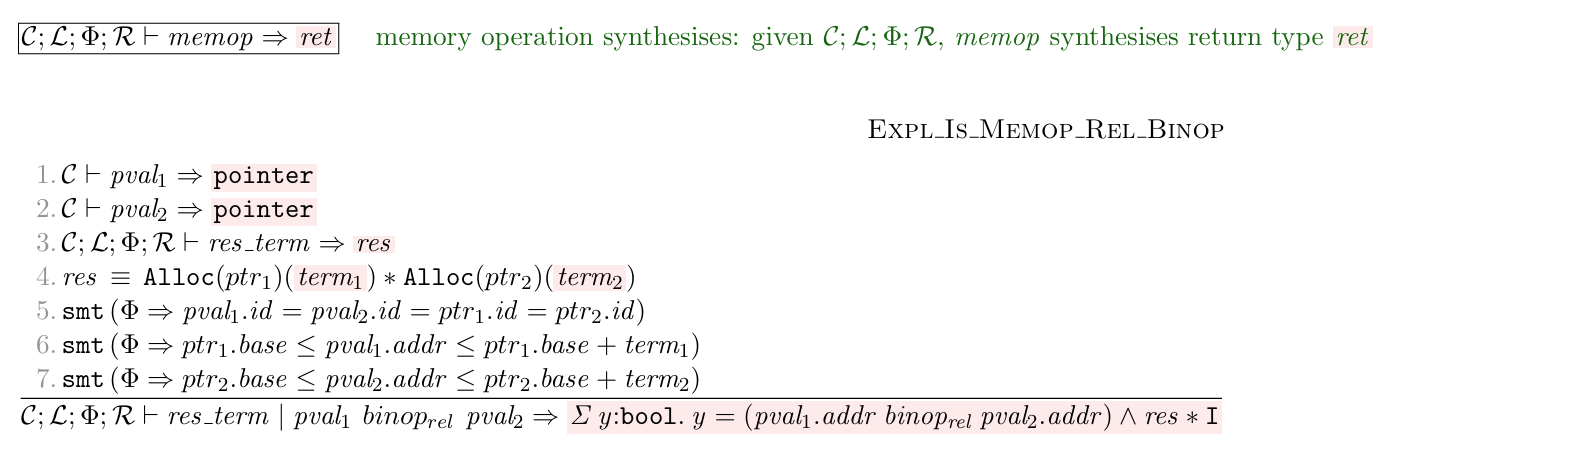
\includegraphics{figures/kernel-memop-typing}
    \caption{\kl{Kernel CN} typing rules for memory actions, and a select rule
        for typing a memory operation.}\label{fig:typing-mem-action}
\end{figure*}

Rules for typing memory operations, i.e.\ `effectful' pointer operations which
require not only for the pointer to be live, but satisfy certain allocation
bounds checks, also synthesise a return type. There are many of them, but they
share the same principles so it suffices to only explain one
(\cref{fig:typing-mem-action}).\sidenote{Update the rule to adjust the pointer
liveness check and notationally simplify the bounds checks into one line.}
Using a binary relational operator (not equality) is only valid if both
pointers are live, belong to the same allocation and have addresses which are
in that allocation's bounds. These constraints are all checked by the SMT
solver, and the return type synthesises the result of that relational operator
applied to the addresses of those pointers, plus any resources consumed to
prove the pointer is live.

\section{Spine judgement}

There are two parts of the grammar which use spine, lists of values. The first
is its typical use in calls to pure Core functions, elaborated C functions, and
effectful Core procedures, as well as to the \coreinline{run()} % chktex 36
operator. Second is the less typical one, in \emph{top-level return values},
usually marked with \coreinline{done()}. So far, I have been showing % chktex 36
how expressions have return types, and so this is how to type the values to
which those expressions step.

Either way, the process for checking them is the same, and so the simplicity
gained by desugaring the \kl{CN} types into kernel types
(\cref{sec:desugaring}) pays off in the straightforward specification of these
rules (\cref{fig:typing-spine}).

\begin{figure*}[tp]
    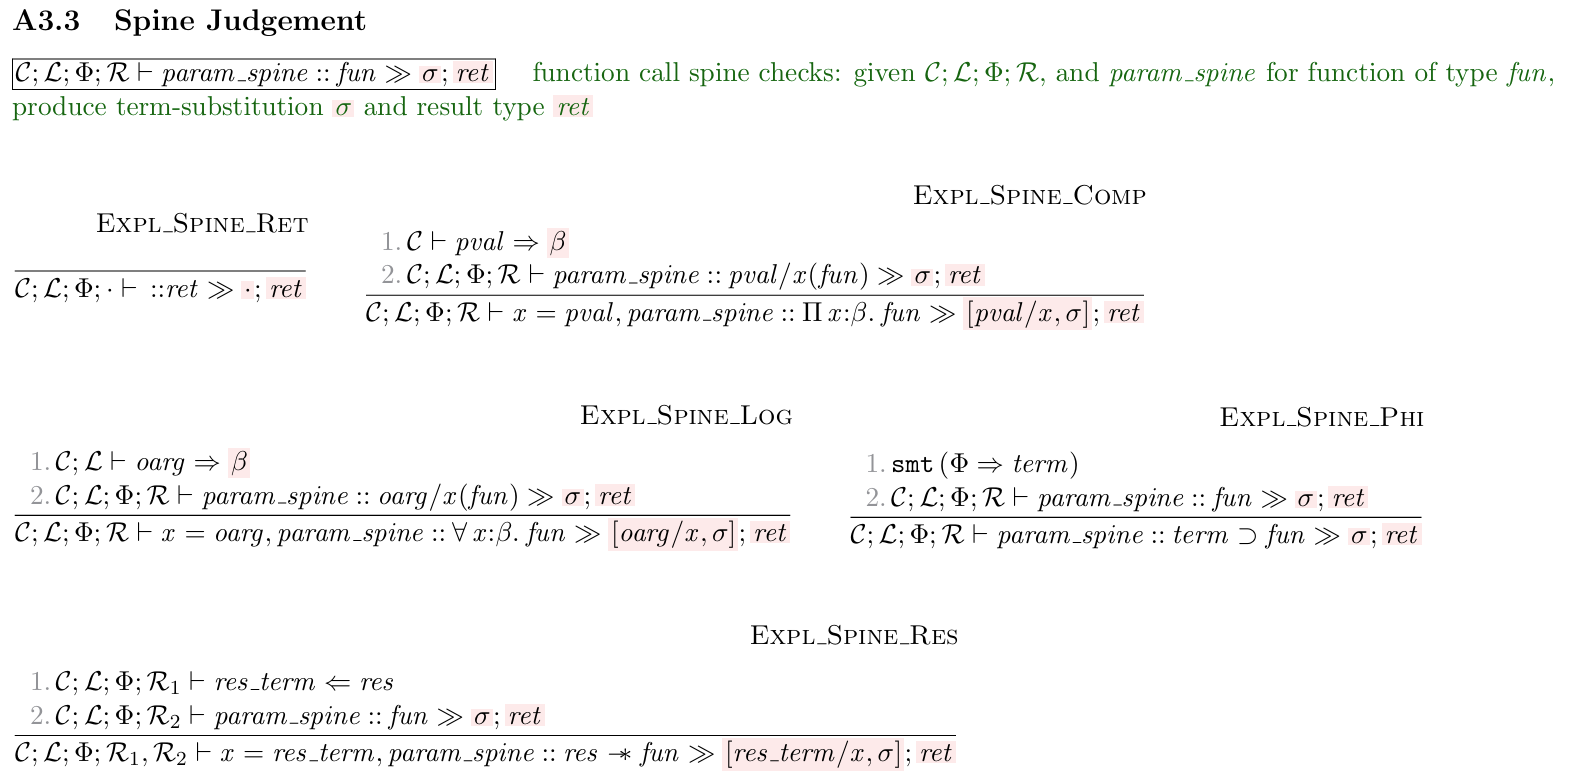
\includegraphics{figures/kernel-spine-typing}
    \caption{\kl{Kernel CN} typing rules for function
        spines.}\label{fig:typing-spine}
\end{figure*}

The judgement for typing spines is $\mathcal{C}; \mathcal{L}; \Phi ;
\mathcal{R} \vdash \mathit{param\_spine} \mathrel{{:}{:}} \mathit{fun} >\!\!>
\outpol{\sigma}; \outpol{ret}$, which means that given the contexts, a spine of
matched-up parameters and arguments and a function type, produce a substitution
$\sigma$ and a return type $\mathit{ret}$.

Function types are dependent over computational and logical (ghost) variables.
For notational convenience, I assume that the variables are the same as the
parameters in the spine. Typing these is done by substituting their
instantiation\sidenote{Remember that for \kl{kernel CN}, I assume all logical
(ghost) quantifiers are explicitly instantiated.} them into the type and typing
the rest of the spine. The substitution produced by this is extended with the
same.\sidenote{Building the substitution this way, rather than
`tail-recursively', made it easier to prove properties about it by induction
(\cref{sec:sub-ctxts}).}\label{sn:tail-rec-sub}. Constraints in types are
simply checked by the calling the SMT solver, and resources in types are
checked by splitting resource context, using one part to type the resource
term, and the other part to type the rest of the function type. Though these
types are not dependent over resources, the terms are, so this rule extends the
produced substitution with one for the resource too.

\section{Effectful values and expressions}

The spine typing is used in the rules for calling elaborated C function
\coreinline{ccall()}, and effectful Core procedures % chktex 36
\coreinline{pcall()}, in \cref{fig:typing-seq-expr-tval}. Both are % chktex 36
syntactically effectful sequenced expressions, typed with a judgement of the
form $\mathcal{C}; \mathcal{L}; \Phi; \mathcal{R} \vdash \mathit{seq\_expr}
\Rightarrow \outpol{ret}$, which says that given the contexts and an effectful
sequenced expression, synthesise a return type. Both lookup a function type for
the called function/procedure,\sidenote{\kl{CN} does not support
computed/indirect function calls, so I assume the callee has already been
resolved.} and simply produce the return type synthesised by the spine
judgement. This is also basically identical to how the top-level value
\coreinline{done<_>} is typed, with the main difference that (a) the judgement
$\mathcal{C}; \mathcal{L}; \Phi; \mathcal{R} \vdash \mathit{tval} \Leftarrow
\mathit{ret}$ is checking (b) the return type must be mapped to its dual
function type before using the spine judgement. Similar to the pure case, the
\coreinline{undef()} and \coreinline{error()} constructs % chktex 36 check
against any type if the constraint context is inconsistent.

\begin{figure*}[tp]
    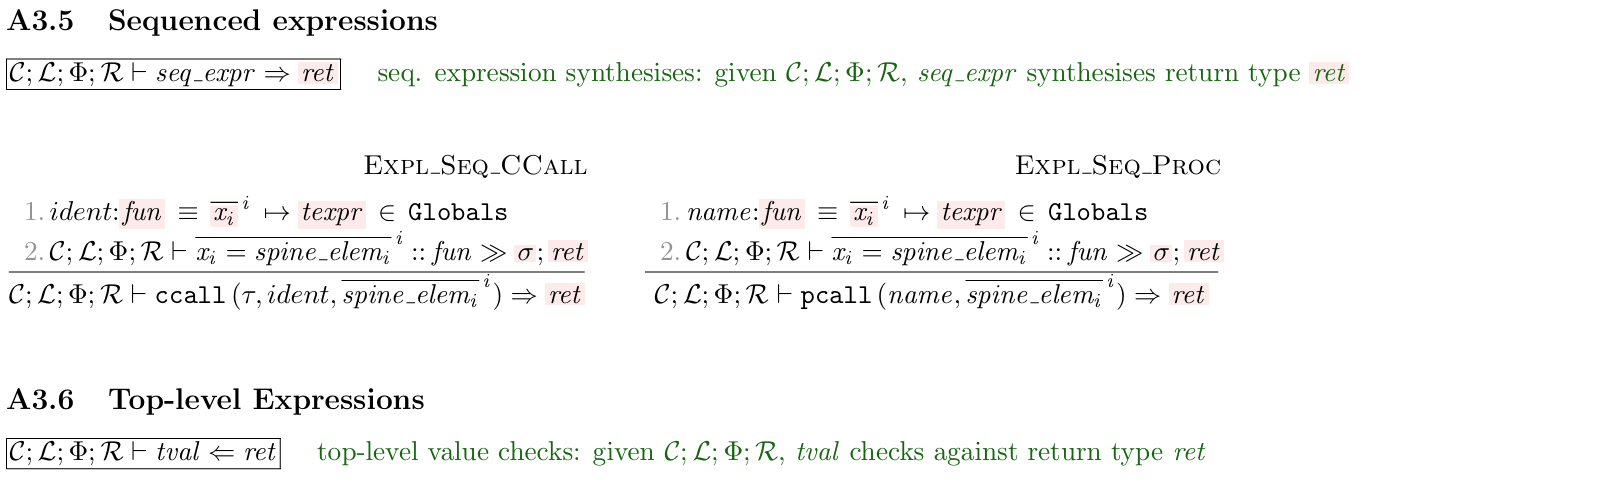
\includegraphics{figures/kernel-seq-expr-typing}
    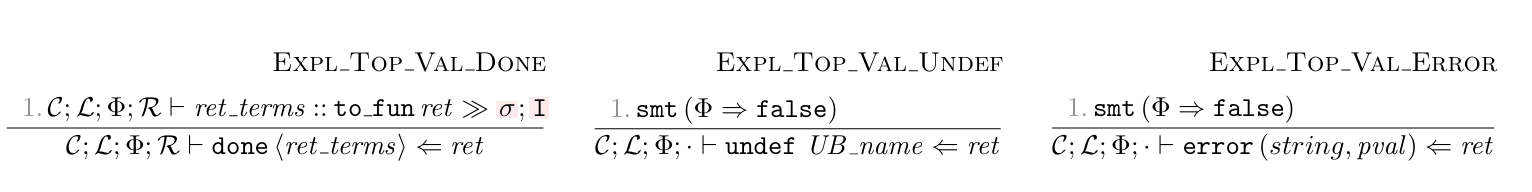
\includegraphics{figures/kernel-tval-typing}
    \caption{\kl{Kernel CN} typing rules for sequential expressions and top-level values.}\label{fig:typing-seq-expr-tval}
\end{figure*}

\section{Pattern matching}

Pattern matching is a surprisingly important crux of \kl{kernel CN}'s type
system because it \emph{is} the canal which directs a rich the grammar of
resource and return types into contexts. The judgement for this is
$\mathcal{C}; \mathcal{L}; \Phi \vdash \mathit{ret\_pat} {:} \mathit{ret}
\rightsquigarrow \outpol{\mathcal{C}'; \mathcal{L}'; \Phi'; \mathcal{R}'}$,
which says that given the contexts, a return pattern and a return type,
synthesise computational, logical, constraint and resource contexts.

Pattern matching for return types (\cref{fig:typing-ret-pat}) is complicated by
the fact that they are dependent on computational and logical (ghost)
variables, and complicated further by the fact that the computational values
have their own patterns (\cref{fig:typing-tpval-tpexpr}).

\begin{figure*}[tp]
    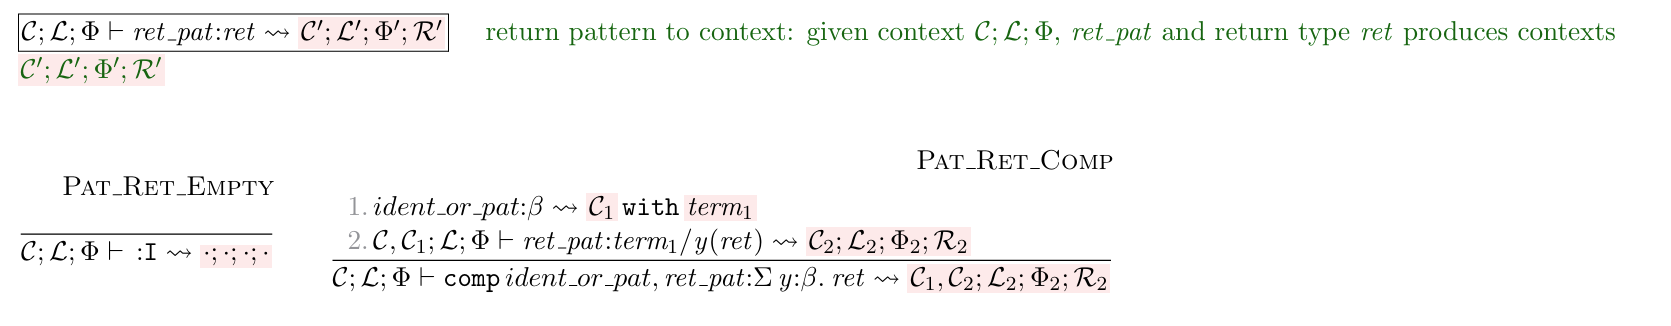
\includegraphics{figures/kernel-ret-pat-typing-1}
    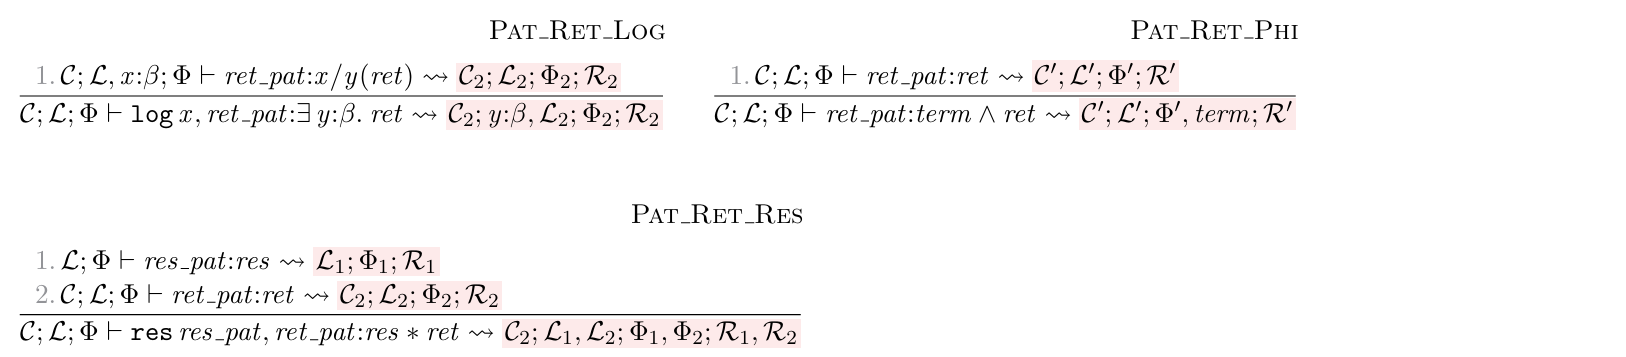
\includegraphics{figures/kernel-ret-pat-typing-2}
    \caption{\kl{Kernel CN} typing rules for pattern matching at return
        types.}\label{fig:typing-ret-pat}
\end{figure*}

If both the head of the type and pattern are computational, the
\textsc{Pat\_Ret\_Comp} rule first uses the heads to synthesise a computational
context $\mathcal{C}_1$ and a represenative $\mathit{term}_1$ of the expected
shape. The former extends the input context, and the latter is substituted into
the the rest of the return type. After the remainder of the pattern is
converted into contexts, it is extended with $\mathcal{C}_1$.\sidenote{Similar
to what I mentioned in note~\ref{sn:tail-rec-sub} about substitution, I build
the contexts this way, rather than `tail-recursively', to make it easier to
prove properties about it by induction (\cref{sec:sub-ctxts}).}

If both the head of the return type and pattern are logical, then context is
extended with the pattern variable,\sidenote{\kl{CN} added support for
algebraic datatypes after I formalised \kl{kernel CN}
(\href{https://github.com/rems-project/cerberus/commit/0e5020732df2ec444ffa7a67abcc7c2c82904d24}{commit
0e50207}) and so and I did not formalise logical pattern matching; I would
formalise it identically to computational pattern matching.} and the same is
substituted into the rest of the return type. Similar to the computational
rule, the synthesised contexts is extended with the pattern variable.

Pattern matching for constraints simply adds the constraint to the contexts
synthesised by the rest of the return type for any pattern. And pattern
matching for resources similarly synthesises combines contexts from both the
resource type and pattern, and the rest of the return type and patterns.

This brings us on to how resource patterns synthesise contexts
(\cref{fig:typing-res-pat}). The judgement for this is $\mathcal{L}; \Phi
\vdash \mathit{res\_pat}{:}\mathit{res} \rightsquigarrow \outpol{\mathcal{L}';
\Phi'; \mathcal{R}'}$, which means that given contexts,\sidenote{I abuse the
notation slightly and omit the computational context $\mathcal{C}$ because it
remains the same in all the rules.} a resource pattern and a type, synthesise
logical, constraint and resource contexts.

\begin{figure*}[tp]
    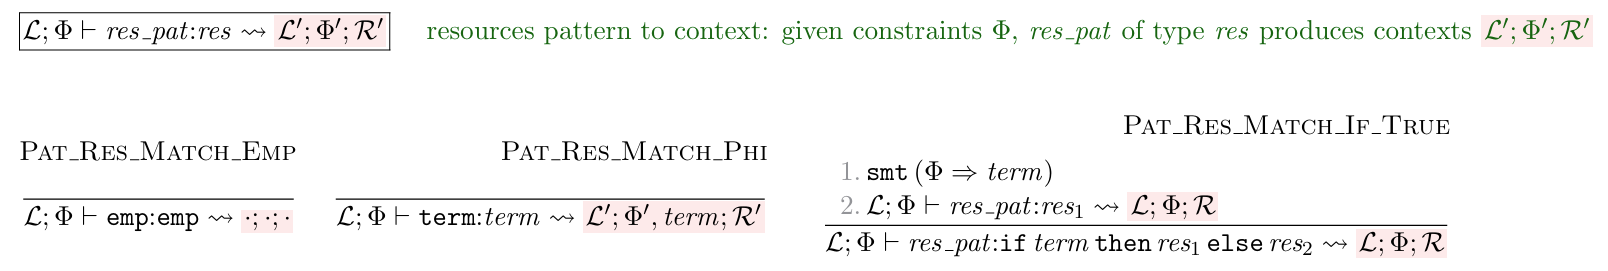
\includegraphics{figures/kernel-res-pat-typing-1}
    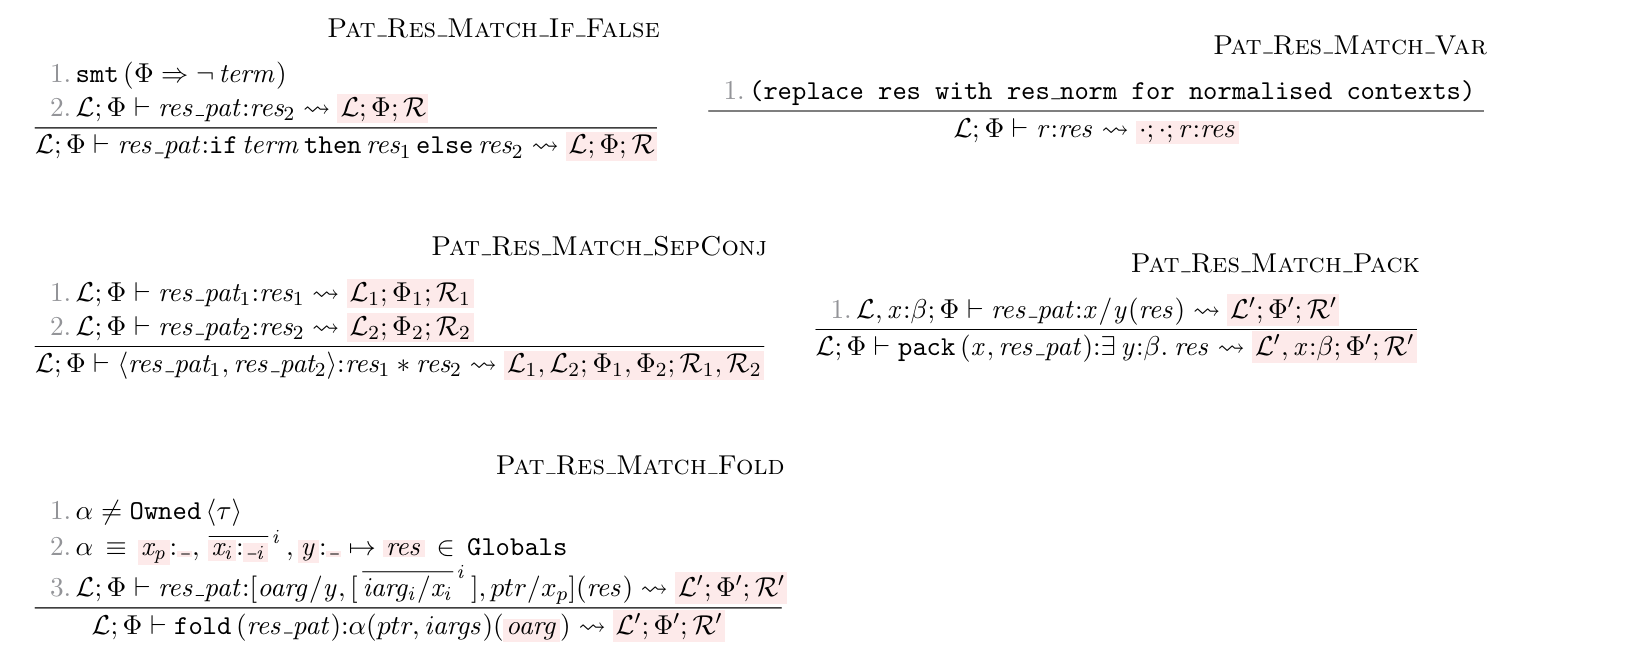
\includegraphics{figures/kernel-res-pat-typing-2}
    \caption{\kl{Kernel CN} typing rules for pattern matching at resource
        types.}\label{fig:typing-res-pat}
\end{figure*}

I am going to focus only on the rules for ordered-disjunctions and folds; the
rest are as expected. For the former, similar to its checking rule, its
condition or its negation must be proven, after which the corresponding branch
against is destructed on the same pattern; dual to its introduction by any
term, it can also be eliminated by any pattern. In the case of
\kl{under-determined} conditions, only the wildcard or the variable pattern
will match against the type. For the latter, the pattern only destructs when
the type is a predicate type and the nested pattern destructs against the
definition of that predicate (with the arguments substituted).

\section{Effectful top-level expressions}

With pattern matching in hand, I can explain the typing rules for effectful
top-level expressions (\cref{fig:typing-seq-texpr}). For space, I will
only talk about \coreinline{let} and \coreinline{run()} expressions, % chktex 36
the remaining rules are as one would expect presented in the appendix.

Top-level expressions are all checked, but the bound expression in the
\coreinline{let} is synthesised, so that the type can be used as part of
destructing the pattern it is bound against to synthesise extra contexts. Those
contexts are then appended to the existing one to check the body of the
\coreinline{let}. As for the \coreinline{run()} operator, the rule % chktex 36
looks up the function type belonging to the label being run, and then checks
that the spine satisfies that function type. Unlike the previous function call
operators, control flow does not return from a \coreinline{run()} % chktex 36
and so the type synthesised is expected to be false, and it checks against any
type.\sidenote{Need to update the rule.}

\begin{figure*}[tp]
    \includegraphics{figures/kernel-seq-texpr-typing-1}
    \begin{minipage}{0.7\textwidth}
        \includegraphics{figures/kernel-seq-texpr-typing-2}
    \end{minipage}
    \begin{minipage}{0.7\textwidth}
    \includegraphics{figures/kernel-seq-texpr-typing-3}
    \end{minipage}
    \caption{Select \kl{Kernel CN} typing rules for effectful top-level
        expressions.}\label{fig:typing-seq-texpr}
\end{figure*}

\section{Elaboration}\label{sec:elaboration}

Part of the \kl{Kernel CN} system also includes a specification for an
\emph{elaboration} system. At the time it was formalised, \kl{CN}
required users to manually fold and unfold predicates\sidenote{I should change
    the formalised grammar to use fold and unfold even though the terms CN used
we pack and unpack.}, but inferred indices for iterated predicates
automatically. Now, CN automatically folds and unfolds predicates but requires
users to state which indices are allowed to be moved in and out of any iterated
predicates in the context.\sidenote{See note~\ref{sn:new-inf-statics}.}
Instantiations for logical quantifiers were and continue to be inferred.

The goal of an elaboration pass over \kl{Kernel CN} is to take as an input a
well-formed program in \kl{ResCore} which has no explicit resources terms and
no instantiations for logical quantifiers on function calls, memory actions or
pointer operations, and to return the same program with the missing pieces
filled in, such that the above typing rules would pass if the program was
successfully elaborated, and fail if there was no elaboration possible.

I do not have a proof of these properties and so I cannot claim that the system
I am about to present meets the above goals. However, it is still useful to
present it, as it highlights some of the challenges in specifying such a system
in the first place; it also clarifies a few points about \kl{CN}'s
implementation (\cref{sec:restriction-branching}).

I shall only present a small slice of the elaboration to highlight the key
concepts, leaving the rest of the large system to the appendix. The main
judgement for synthesising a resource term and an instantiation for a logical
quantifier is $\Phi; \underline{\mathcal{R}} \vdash \mathtt{calc}\; y \;
\mathtt{using} \mathit{res} \rightsquigarrow \mathtt{bind}\;
\outpol{res\_bind}\; \mathtt{for} \outpol{res\_term} \; \mathtt{and} \;
\outpol{oarg} \dashv \outpol{\underline{\mathcal{R}'}}$
(\cref{fig:elab-res-oarg}). Given a constraint context, a resource context, an
output parameter, and a resource type, synthesise a series of bindings for an
output argument and resource term and which will result in the updated resource
context.

\begin{figure*}
    \includegraphics{figures/kernel-elab-calc-1}
    \includegraphics{figures/kernel-elab-calc-2}
    \includegraphics{figures/kernel-elab-calc-3}
    \caption{Select \kl{Kernel CN} rules for an elaboration pass which given
        contexts and a resource type, infers proof terms and logical quantifier
        instantiations satisfying those types.}\label{fig:elab-res-oarg}
\end{figure*}

\subsection{Normalised resource contexts}\label{sec:norm-ctxt-res}

One of the key restrictions I place to allow inference to be specified
relatively simply is that of a \intro{normalised} resource context, signified
with an underlined $\underline{\mathcal{R}}$, containing only normalised
resources types. A normalised resource is either an (iterated) predicate, or an
under-determined conditional resource. I call it normalised because (with the
appropriate terms and pattern-matching), any resource context can be
manipulated into such a normal form. This means it is simple to specify lookups
in the context: if I need $b \astRef{} c$ but the context has $\{\; x : a
\astRef b , y : c \astRef{} d \}$ then how should I proceed? Do I lookup $b$
and $c$ individually? Together? Swapped? How do I handle the case where one is
a sub-resource of a resource in the context? I avoid these questions and simply
require that other judgements which use resource lookup (all of them) simply
preserve normality as an invariant. This requires constructing rebindings of
existing terms (\cref{fig:res-bind-def}) to manipulate the context, carefully
retaining `leftover' resources from a lookup.

\begin{marginfigure}
    \includegraphics{figures/kernel-res-bind-def}
    \caption{\kl{Kernel CN} definition of resource bindings Note that these are
        only required in the presence of explicit resource terms, and as such
        are not necessary in \kl{CN}'s implementation.}\label{fig:res-bind-def}
\end{marginfigure}

\subsection{Synthesising resource terms and output arguments}

The judgement for synthesising resource terms and output arguments relies on
the fact that the more flexible \kl{kernel CN} types (\cref{fig:kernel-res})
have come from a translation (\cref{fig:pred-to-kernel}) of the intentionally
rigid surface syntax (\cref{sec:monadic-syntax}). Synthesising a term for
$\mathsf{emp}$ is simple and does not change the context, and the synthesised
output argument is just a dummy value.

Synthesising an output argument from equality constraints\sidenote{Should
update the rule to use a single one.} is just taking the right-hand-side of the
equality. Synthesising a resource term and an output argument for a
ordered-disjunction requires proving the condition or its negation, and then
synthesising the appropriate branch. For under-determined conditions, as
mentioned in~\nameref{subsec:checking-res-terms}, the term must be a variable
from the resource context whose type matches syntactically, modulo SMT
provability.

By construction, every existential quantifies over the output argument of
(iterated) predicates, and so synthesising a resource term and an output
argument for the \emph{whole} requires synthesising the output argument of the
(iterated) predicate. That it in turn, may require inferring an index to the
resource from an iterated version, which is handled by a separate judgement.
The inferred argument is substituted into the rest of the resource type to
infer another resource term and the originally requested output argument. The
synthesised resource term simply pairs and packs the aforementioned two, whilst
the synthesised output argument is the \emph{second} one (the first one was for
the existential).

\subsection{Synthesising indices for iterated predicates}\label{subsec:synth-indices}

Inferring indexes was possible, and relatively straightforward, because of the
requirement that every predicate had as its first input argument a pointer $p$,
and that every iteration over index $i$ of such predicates had as its first
argument $p +_\mathrm{ptr} i * \mathit{step}$ where $\mathit{step}$ is some
constant integer. Given these, inferring an index (for either
\coreinline{break}ing or \emph{glue}ing) reduced to $i = (p' - p) /
\mathit{step}$ where $p'$ is the pointer in the first argument of the request
predicate. This is made precise in \cref{fig:res-diff-break}.\sidenote{This
allows for empty iterated remainder: change it?}  The judgement $\Phi \vdash
\mathit{ident}{:}\underline{\mathit{res}} \mathbin{{-}?} \mathit{res\_req}
\rightsquigarrow \outpol{res\_diff}$ says that given constraint context, a
\kl{normalised} resource,\sidenote{Predicate (iterated) or an under-determined
ordered-disjunction.} and a request for a predicate (iterated), synthesise the
`difference' between the two. As shown in \cref{fig:res-diff-def}, the
`difference' can be of four sorts: no difference, exact match, subset match,
overlapping match and each requires slightly different handling (continue
search, stop search, bind remainder and stop search, bind remainder and
continue search respectively) from the lookup judgement (in appendix).

\begin{marginfigure}
    \includegraphics{figures/kernel-elab-res-diff-def}
    \caption{\kl{Kernel CN} definition of a `resource difference'. The second
        `and' needs to be changed to a `rem'.}\label{fig:res-diff-def}
\end{marginfigure}

\begin{figure*}[tp]
    \includegraphics{figures/kernel-elab-diff-1}
    \includegraphics{figures/kernel-elab-diff-2}
    \caption{Select \kl{Kernel CN} elaboration rule for inferring indices and
        synthesising predicate operations.}\label{fig:res-diff-break}
\end{figure*}

\subsection{Using elaboration judgements}

It is important to note that the `calc' judgement synthesises a checking
resource term, and so care must be taken for it to be used in a checking
position. The main place this judgement is used however was for manually
folding predicates (\cref{fig:kernel-elab-fold}), which by accident of \kl{CN}'s
original implementation was in a synthesis position in the grammar rather than
a checking one (hence the type annotation on folding resource
terms,~\cref{subsec:synth-res-term}). The judgement is similar to a
synthesising typing judgement, but in addition to synthesising a return type,
it also synthesises a list of resource bindings to manipulate the context, and
an elaborated expression containing the fold resource term with several type
annotations to engineer into a synthesis form.

\begin{figure*}[tp]
    \includegraphics{figures/kernel-elab-fold-1}
    \includegraphics{figures/kernel-elab-fold-2}
    \caption{\kl{Kernel CN} elaboration rule for manually folding
        predicates.}\label{fig:kernel-elab-fold}
\end{figure*}

All other placements of resource terms only require (iterated) predicates, such
as memory actions like \coreinline{load} (\cref{fig:elab-action}) and spines
(\cref{fig:elab-spine}) for calls to elaborated C functions and Core
procedures. In these cases we see that the output argument is used only in
return types\sidenote{The synthesised return types are used in turn to
synthesise patterns to maintain the invariant that the resource context is
always normalised.} but that the resource terms (and the resource bindings
which precede it to manipulate the context into the right form for typing these
terms) are the main things elaborated into the program.

\begin{figure*}[tp]
    \includegraphics{figures/kernel-elab-action-1}
    \includegraphics{figures/kernel-elab-action-2}
    \caption{Select \kl{Kernel CN} elaboration rule for memory
        actions.}\label{fig:elab-action}
\end{figure*}

\begin{figure*}[tp]
    \includegraphics{figures/kernel-elab-spine-1}
    \includegraphics{figures/kernel-elab-spine-2}
    \caption{\kl{Kernel CN} elaboration rule for instantiating a logical
        quantifier when elaborating a function call spine.}\label{fig:elab-spine}
\end{figure*}

\chapter{Kernel CN:\ Proof of soundness}%
\label{chap:kernel-soundness}

To ensure that \kl{Kernel CN} had served as a useful formalisation for \kl{CN},
I proved that it was sound. The whole proof is large and in the appendix; In
this chapter, I will discuss the key definitions, lemmas and proof sketches. I
will first define an operational semantics for \kl{ResCore}, and then do a
straightforward, if not slightly tedious, syntactic proof of type
safety.\sidenote{The continuation-like behaviour of the \coreinline{run()} % chktex 36
and \coreinline{save()} operators make it more challenging to prove % chktex 36
soundness in a denotational manner.} This suffices because \kl{ResCore} is a
first-order language, and all functions and labels are annotated with the
correct type,  despite the presence of linear types, which usually require
logical relation methods.

The proof is split up into three smaller proofs: a joint
progress-and-type-preservation proof for resource term reduction, a progress
theorem, and a type-preservation theorem.

The definitions and lemmas of note in this proof are (a) the careful definition
of substitution, and its accompanying substitution lemma (b) the novel
structure of the heap, which is unusual in that is essentially just separation
logic predicate (c) the interaction between the resource terms and heaps.

\section{Substitution and contexts}\label{sec:sub-ctxts}

The first three rules for typing substitutions (\cref{fig:soundness-sub}) are
simple enough: the empty substitution represents the empty context, a
computational or logical substitution requires the substituted value to be well
typed, and same for the resource term. However, because resource terms and
types can depend on the first two, scoping needs to be handled carefully,
so resource types in a substitution may only mention variables
either in the contexts on the left of the turnstile, or the computational
and logical context in the substitution type. This makes it easier to decompose
substitutions into valid parts, each of which can be applied sequentially but
still produce a meaningful results (because of the dependent types,
substitutions may be telescoping, so need not commute). Hence, the
\textsc{Sub\_Chk\_Concat} rule checks not only the first half $\psi$ of the
substitution against half the context, but checks the second half
\emph{substituted} against second half of the context \emph{substituted}, to
eliminate any mention of variables from $\mathcal{C}_1$ and $\mathcal{L}_1$ in
$\mathcal{R}'_2$.

\begin{figure*}[tp]
    \includegraphics{figures/kernel-soundness-sub-1}
    \includegraphics{figures/kernel-soundness-sub-2}
    \caption{\kl{Kernel CN} substitution typing}\label{fig:soundness-sub}
\end{figure*}

In the appendix, I use this definition to prove lemmas such as substitution
preserves SMT results and that substitutions can be split up (linearity means
this property is not completely trivial). The key lemma is the substitution
lemma stated below.

\begin{lemma}[Substitution lemma]
If $\mathcal{C}'    \mathcal{L}'  ;  \Phi  ;  \mathcal{R}'  \vdash  J$,
then $ \forall \ \mathcal{C}, \mathcal{L}, \mathcal{R}, \sigma.\
\left( \mathcal{C}    \mathcal{L}  ;  \sigma  (  \mathrm{ \Phi }  )  ;
\mathcal{R}  \vdash  \sigma  \Leftarrow  (  \mathcal{C}'  ;  \mathcal{L}'  ;
\mathcal{R}'  ) \right)  \Rightarrow \allowbreak
\mathcal{C}    \mathcal{L}  ;  \sigma  (  \Phi  )  ;  \mathcal{R}  \vdash  \sigma ( J ) $.
\\[\baselineskip]
If a judgement holds under some context, and the context is the type of
a substitution in \emph{another} context, then the judgement is also holds in
that other context substituted appropriately.
\\[\baselineskip]
Since $\Phi$ is scoped to $\mathcal{C}' ;
\mathcal{L}'$, we must substitute over it as well as all the usual suspects on
the right.\sidenote{I think this slightly off, $\mathcal{R}'$ is scoped the
same too and should need substituting as well.}
\\[\baselineskip]
Substitution of contexts is defined by substituting over each constraint in
$\Phi$. As a result, $\sigma (\Phi_1, \Phi_2) = \sigma (\Phi_1) , \sigma (\Phi_2) $,
and if $\sigma (\Phi) =  \Phi'_1 , \Phi'_2$ then $\exists \Phi_1,  \Phi_2 . \:
\sigma (\Phi_1, \Phi_2)   = \sigma (\Phi_1), \sigma (\Phi_2)$.
\end{lemma}

\begin{proof}
Full proof in the appendix. Induction over the typing judgements. There are
four parts to this proof.
\begin{itemize}
\item \textbf{Variable rules.} Repeatedly invert the substitution typing
    assumption until the variable used in the context appears, and then
    use the equational properties of substitution and the assumptions
    to prove the goal.
\item \textsc{Expl\_Top\_Val\_Done}. $\mathtt{to\_fun}$ commutes with
    substitution, but leaves terms unchanged, so induction proceeds
    straightforwardly.
\item \textbf{Context change rules.} Split up substitutions as required by the
    restrictions on the resource context. If a rule uses the SMT judgement, use
    the substitution preserves SMT results lemma.
\item \textbf{Remaining rules}. Straightforward induction.
\end{itemize}
\end{proof}

\section{Heaps and their types}\label{sec:heap-types}

Heaps in the operational semantics are, slightly unusually, tree-shaped
collections of predicates (\cref{fig:kernel-heap-def}). The leaves of the tree
are the built-in ownership and allocation predicates; the branches of the heap
are predicates tagged with their definition (a resource value of the type of
the predicate body) and a sub-heap (of the resources used by the definition).

\begin{marginfigure}
    \includegraphics{figures/kernel-dynamics-heap-1}
    \includegraphics{figures/kernel-dynamics-heap-2}
    \includegraphics{figures/kernel-dynamics-heap-3}
    \caption{\kl{ResCore} dynamics heap definition.}\label{fig:kernel-heap-def}
\end{marginfigure}

Resource \emph{values} are the subset of resource terms which cannot reduce
further (\cref{fig:kernel-res-val-def}). This is to capture the idea that
predicates encapsulate their contents until opened.

\begin{marginfigure}
    \includegraphics{figures/kernel-dynamics-res-val}
    \caption{\kl{ResCore} resource \emph{values} (subset of terms).}\label{fig:kernel-res-val-def}
\end{marginfigure}

This means that, in the dynamic semantics, folding (and via pattern matching,
unfolding) predicates \emph{affect the shape of the heap}
(\cref{fig:kernel-fold-unfold}). In the unfold rule, the nested definition is
used to destruct the rest of the pattern into a substitution, and the heap is
extended with the sub-heap associated with those values.

\begin{marginfigure}
    \includegraphics{figures/kernel-dynamics-unfold}
    \includegraphics{figures/kernel-dynamics-fold}
    \caption{\kl{ResCore} dynamics for folding and unfolding
        predicates.}\label{fig:kernel-fold-unfold}
\end{marginfigure}

In the fold rule, the inverse happens, which requires splitting a heap into the
\emph{footprint} of some resource values, and the remainder
(\cref{fig:kernel-footprint}). I define the footprint of a resource value as
the sub-heap containing the (iterated) predicates referred to in said value.

\begin{figure*}
    \includegraphics{figures/kernel-dynamics-footprint-1}
    \includegraphics{figures/kernel-dynamics-footprint-2}
    \caption{\kl{ResCore} dynamics definition of a footprint of a resource
        value in a heap.}\label{fig:kernel-footprint}
\end{figure*}

I defined both the pattern matching and the resource term reduction dynamic
semantics in a big-step style; this makes the definition of both more concise,
at the cost of intertwining the usually separate proofs of progress and type
preservations for resource term reduction.

The final definition required for the proof is that of the type of a heap. The
type of a heap is a \kl{normalised resource} context
(\cref{sec:norm-ctxt-res}); the rules for these are straightforward
(\cref{fig:kernel-heap-typing}), except the fact a heap with a folded predicate
requires there exists a context for which the resource value $[[ def ]]$ and
$[[ heap ]]$ is well-typed. This becomes necessary for proving the progress of
pattern-matching for the whole of the annotated and let-normalised Core.

\begin{figure*}
    \includegraphics{figures/kernel-heap-typing}
    \caption{Select typing rules for heaps.}\label{fig:kernel-heap-typing}
\end{figure*}

As with elaboration, using normalised resource contexts does not restrict the
generality of progress and type preservations theorems.This is because of the
following lemma: if a well-typed resource term is closed, then the context in
which it is well-typed must normalised (formal definition and proof in the
appendix). We now have all the ingredients to state and sketch a proof for the
progress and type preservation for resource terms.

\begin{theorem}[Progress and type preservation for resource terms]
For all closed resource terms ($[[ res\_term ]]$) which type check or
synthesise ($[[ cdot ; cdot ; N ; nR |- res\_term <= res ]]$) and all well-typed
heaps ($[[ N |- h <= nR ]]$) there exists a resource value ($[[ res\_val ]]$),
context ($[[ nR' ]]$) and heap ($[[ h' ]]$), such that: the value is
well-typed ($[[ cdot ; cdot ; N ; nR' |- res\_val <= res ]]$); the heap is
well-typed ($[[ N |- h' <= nR' ]]$); for all frame-heaps ($[[ f ]]$), the
resource term reduces to the resource value without affecting the frame-heap
($[[ < h + f ; res\_term > ||v < h' + f ; res\_val > ]]$).
\end{theorem}

\begin{proof}
Full proof in the appendix. Induction on the resource
term typing assumption. The type dictates the value and context, the latter of
which dictates the shape of the heap; all of this relies heavily on a few
inversion lemmas. The existential is necessary later for proving well-typed
values pattern pattern match successfully, where it is used as a witness when
proving heap typing for folded predicates. The frame heap $f$ is necessary later
for proving type preservation for \coreinline{let}-expressions.
\end{proof}

\section{Soundness}

The configuration for the operational semantics is a pair of a heap and a
ResCore program. As one might expect, proving progress requires well-typed
patterns successfully produce substitutions. I assume that all computational
patterns are exhaustive, because if they are not, this is a bug in Cerberus.
Proving well-typed patterns successfully produce substitutions is complicated
by two things, the solution to which requires the introduction of a relation on
SMT terms and resource types, $[[ N |- res \~ res' ]]$ (to be read ``under
constraints $[[ N ]]$, $[[ res ]]$ is related to $[[ res' ]]$'').

The first is that the constraint term generated when typing a computational
pattern (this is required to record, in the constraint context, which branch
the type system is assuming it is in) is not exactly equal to the values it can
match in the operational semantics (nor would we want it to be: the pattern $[[
Cons ( x1 , x2 ) ]]$ should match the value $[[ Cons ( pval1 , Cons ( pval21 ,
Nil base\_type ( ) ) ) ]]$). Hence, we must weaken the notion of equality on
types to $[[ \~ ]]$ relatedness, which links the two, so that during the proof,
we can substitute the constraint term $[[ x1 cons x2 ]]$ at the type-level, and
maintain a link to the corresponding value.

The second is that the conditions of related ordered-disjunctions must remain
SMT-equivalent (with reference to a constraint context), so that pattern-match
typing and resource term typing are consistent.

\begin{theorem}[Progress for the annotated and let-normalised Core]
If a top-level expression ($[[ texpr ]]$) is well-typed
($[[ cdot ; cdot ; N ; nR |- texpr <= ret ]]$) and all computational patterns
in it are exhaustive, then either it is a value ($[[ tval ]]$), or it is
unreachable, or for all heaps ($[[ h ]]$), if the heap is well-typed
($[[ N |- h <= nR ]]$) then there exists another heap ($[[ h' ]]$) and expression
($[[ texpr' ]]$) which is stepped to ($[[ < h ; texpr > --> < h' ; texpr' > ]]$)
in the operational semantics.
\end{theorem}

\begin{proof}
Induction over the typing assumption. Full proof in appendix.
\end{proof}

Moving on to type preservation, a few things are noteworthy about its proof.

First is that a frame-heap has to be explicitly passed around.  Whilst this is
inconvenient, it becomes necessary in the \textsc{Expl\_Top\_Seq\_LetT} case.

Second is in the lemma ``Well-typed values pattern match successfully''.%\nameref{subsec:wt_values_pat_match}.
There are two substitutions at play here. As an example, let
the value being matched be $[[ Cons ( Unit , Nil unit ( ) ) , ret\_terms ]]$ and
the pattern be $[[ comp Cons ( x1 : unit , x2 : list unit ) , ret\_pat ]]$.
For the return type $[[ sigma y : list unit . ret ]]$, the type-level
substitution will be $[[ Cons ( x1 , x2 ) / y ( ret )]]$.  However, at the
term-level, the substitution will be $[[ [ Unit / x1 , Nil unit ( ) / x2 ] ]]$.
\emph{Bridging this difference is the main reason for the $[[ ~ ]]$ relation}
(the other is the use of $[[ to\_fun ret ]]$).  \emph{The type-level substitution
is open}, and only makes sense with respect to the variables introduced in the
pattern-match.

Lastly, we gather constraints throughout the proof, since these are accumulated
by the typing rules, during pattern-matching, case and if. Given the constraint
context is always well-formed
% VIP related (w.r.t.~to the initial logical variable context $[[ L0 ]] = [[ allocv : id\_map ]]$), this means that after substituting in the
allocation history, all the constraints involve no variables
% VIP related (hence the substitutions in \textsc{Heap\_Ty} and \textsc{Alloc\_Ty})
, and so will be trivially decidable.

\begin{theorem}[Type preservation for the annotated and let-normalised Core]
For all closed and well-typed top-level expressions
($[[ cdot ; cdot ; N ; nR |- texpr <= ret ]]$),
well typed heaps ($[[ N |- h <= nR ]]$),
frame-heaps ($[[ f ]]$),
new heaps ($[[ heap ]]$),
and new top-level expressions ($[[ texpr' ]]$),
which are connected by a step in the operational semantics
($[[ < h + f ; texpr > -->  < heap ; texpr' > ]]$),
if all top-level functions are annotated correctly,
there exists a constraint context ($[[ N' ]]$),
sub-heap ($[[ h' ]]$),
and resource context ($[[ nR' ]]$),
such that the constraint context is $[[ N ]]$ extended,
the frame is unaffected ($[[ heap ]] = [[ h' + f ]]$),
the sub-heap is well-typed ($[[ N' |- h' <= nR' ]]$),
and the top-level expression too
($[[ cdot ; cdot ; N' ; nR' |- texpr' <= ret ]]$).
\end{theorem}

\begin{proof}
Induction over the typing assumption. Full proof in appendix.
\end{proof}

\chapter{Informing implementation discussions}\label{chap:inform-impl}

In the early stages, \kl{CN} was implemented by Christopher Pulte and Thomas
Sewell, based on sketches by Neel Krishnaswami. I started formalising
\kl{Kernel CN} much later, and benefited by the clarity of having an
implementation and implementers I could consult in moments of
confusion.

However, this mode of development means that there were \emph{many} design
decisions made in a rather conservative context, because the programming was
always of a system which was being defined along the way, rather than a
well-understood pre-existing one. Extensions to syntax and inference were
always the minimum required for verifying the pKVM buddy allocator, lest
performance and inference suffer greatly, rather than ones based on a strong
formal and holistic consideration of the constructs and interactions at play.

As such, there are several restrictions in the implementation, which with the
benefit of hindsight and formalisation, are completely unnecessary, but persist
as technical debt. This chapter lists a few of these, and explains how the
formalisation brings much needed clarity to many questions around the
implementation.

\url{https://github.com/rems-project/cerberus/labels/language}
\url{https://github.com/rems-project/cerberus/labels/resource\%20reasoning}

\section{Supporting partially initialised reads of structs/unions}\label{sec:partial-init-structs}

So far in working on verifying the buddy allocator, writing a tutorial and
working with our industry partners, no code has needed the ability to read a
partially (including completely) uninitialised struct/union, and any valid code
which does this would have to simply ignore that result. The \kl{UB} only comes
when one tries to read an uninitialised primitive type member of the
struct/union from that earlier read.

Because we can decompose ownership of a struct into its fields, and track the
initialised status of those individually (perhaps verbosely for large structs),
it does not seems like we lose much in expressiveness in forbidding this. The
only valid code that would be additionally rejected if this was forbidden in
the type system would be a read of a partially initialised struct followed by a
call to a function which reads only the initialised fields. And in such
instances, it seems likely that the code could be refactored to only pass the
initialised fields, or a pointer with the appropriate precondition to only read
the initialised fields.

Although we wish to verify C code as is, because programmers need to change the
``code'' to write annotations anyway, such small, rare and easy to explain
refactors are a worthwhile trade-off if it makes the design and implementation
of \kl{CN} simpler. The book-keeping for tracking initialised status in
symbolic terms, rather than in a flag the name of a predicate, adds a
non-trivial amount of noise to formalisation and would do the same in the
implementation.

Perhaps such an allowance simplifies data-flow analysis inside a compiler, so
that it may safely ignore the values resulting from a load of partially
uninitialised loads of a of struct, so long as none of the fields are accessed.
It seems hard to think of a case for this allowance motivated by performance or
programmer ergonomics, and so the experience from formalising this suggests
that the current implementation of \kl{CN}, which does not allow loads from
partially (including completely) uninitialised structs, can and will remain
expressive enough for all of its use cases.

\section{Auto unfolding scheme for logical functions}\label{sec:auto-unfold-functions}

\url{https://github.com/rems-project/cerberus/issues/483}

One of the strange parts of working with \kl{CN} is the predicate definitions are
automatically unfolded but not logical functions, even though both may be
recursive. As such there is separate and cumbersome annotation to manually
unfold a function.

The way the implementation determines whether to unfold a predicate is
to always unfold it if there is no top-level if, or to check if the condition
or its negation can be proven before unfolding the corresponding branch.

However, with the benefit of the formalisation, we can see that those are
actually two orthogonal questions, which happen to be tied together because of
historical reasons. In the formalisation (\cref{fig:typing-res-pat}), including
the elaboration rules (\cref{fig:kernel-elab-fold}),  we can see that (un)folding % chktex 36
predicates does not require calling the SMT solver, but determining which
branch of an ordered-disjunction to check does.

So not only does this suggest loosening the restrictions on branching in
predicate definitions (\cref{sec:restriction-branching}), it also suggests that
the general approach of ``unfold until you reach a condition for which neither
it nor its negation can be proven'' would work for logical functions too.

It is important to note that with automatic constraint-based unfolding, it is
possible for users to write constraints (including via control flow) which make
\kl{CN} diverge, and at this stage it is unclear how any well-foundedness
checks on the definitions of predicates would prevent this particular failure
mode.\sidenote{\url{https://github.com/rems-project/cerberus/issues/451}}

\section{Higher-order resources}
\url{https://github.com/rems-project/cerberus/issues/363}

If we want \kl{CN} to be used in real-world settings, it must support
concurrency. We can use the formalisation to reflect on what changes
would be needed to support this.

Fractional permissions would be useful to enable sharing. After that,
the issue becomes what level of support would be useful and worth implementing
based on the size of the change.

For example, hard-coding support for locks as an extra kind of resource would
be relatively straightforward (adding more terms and operations to the
grammar), but adding support for higher-order resources in general, so that
locks can be defined rather than an built-in feature, would be substantial
change to the resource type definitions and rules.

\section{Restrictions on branching}\label{sec:restriction-branching}
\url{https://github.com/rems-project/cerberus/issues/483}
\url{https://github.com/rems-project/cerberus/issues/266}

As mentioned in~\nameref{sec:auto-unfold-functions}, the formalisation
separates out two features (unfolding definitions, and selecting a branch of an
ordered-disjunction) which are tied together in the implementation. One of
the other places this shows up is in a restricted syntax for predicate definitions:
they must either have no ordered-disjunctions, or only one, placed first at the
top-level.

With the formalisation, not only can I show that that restriction is
unnecessary, I can also shed light on how to change the implementation to lift it.

This is because I can argue that the surface syntactic restriction and the
internal representation of predicate definition are actually two
\emph{orthogonal} issues. The key insight here is that this feature does not
add any extra expressive power, it simply unbundles to features which are
orthogonal in the formalisation. Indeed, users can work around the restriction
by manually defining an extra auxiliary predicate each time they wish to use an
ordered-disjunction anywhere which is not first and at the top-level, it is just
clunky.

This orthogonality extends to implementing fixes for this issue too
\textemdash{} I can sketch out two ways of lifting this restriction in the
implementation and offer those options, with their own trade-offs, to other
developers and users to decide which, if any, is preferable.

\section{Removing the pointer first restriction on predicates}\label{sec:rm-ptr-first}
\url{https://github.com/rems-project/cerberus/issues/303}

Another awkward restriction in working with \kl{CN} is that the first argument
to a predicate must always be a pointer. This is usually fine because it would
be strange to speak of ownership without a pointer, but the pointer is derived
from elsewhere (a fixed base pointer, but a given index), or sometimes the
pointer is in a record and that is the easiest thing to pass in.

With the formalisation, we can estimate the impact of removing this restriction
and see that the main thing we would lose is not in terms of typing fewer
programs, but in terms of synthesising indices for manipulating iterated
predicates (\cref{subsec:synth-indices}). Given that \kl{CN} has already moved
away from inferring those,\sidenote{See note~\ref{sn:new-inf-statics}.} we can
conclude that removing this restriction will not diminish the automation or the
expressive power of \kl{CN}.\sidenote{It will not increase expressiveness
either, because users currently can and do just use a dummy parameter.}

\section{Unifying the syntax of functions, predicates and specifications}

\url{https://github.com/rems-project/cerberus/issues/304}

Syntax is part of the user-interface of \kl{CN}, and as such it is subject to
strong constraints, strong scrutiny and strong opinions.

Currently, logical (ghost) functions and predicates are separated (represented
by different OCaml types) in the implementation. This is with good reason:
the pure parts are shipped off to an SMT solver, but the heap parts are the
domain of the resource reasoning. However, \kl{CN} also enforces this
distinction syntactically, which is a perfectly valid choice, but it trades
concision and occasional confusion when those worlds need to mix, for clarity
in separating when the two do not.\sidenote{\url{https://github.com/rems-project/cerberus/issues/288}}

Another equally valid choice would be to unify the two syntaxes and find some
other way of enforcing the necessary distinction between the two worlds.
Exposing the monad implicit in the predicate syntax as a type constructor would
achieve both, though at the cost of exposing developers to a fancier type
system. As a programming-language theorist, I prefer this, though the ultimate
arbiter of such a decision would have to well-designed user-studies.

\chapter{An alternative presentation}\label{chap:kernel-alternative}

I will conclude this part by sketching out an alternative presentation of the
\kl{CN} type system, \intro{MiniCN}, closer to both C as a surface language and
the \kl{CN} implementation. It will demonstrate the challenges of \emph{not}
using \kl{ResCore}, due to it not being a first-order functional
language with explicit resources and let-normalisation. The former means the
inference cannot be specified separately, whereas the latter in particular
complicates typing early-returns and join-points. It will also demonstrate the
challenges which seem to be inherent to designing a type system for a C-like
language.

\section{MiniC and MiniCN}

\kl{MiniC} is a C-like language intended to capture the parts of C relevant to
explaining the core ideas behind
\intro{Fulminate}\sidecite{banerjee2025fulminate}, a separation-logic testing
framework which translates \kl{CN} specifications to C. It includes global
variables, mutable function paramaters, block-scoped local variables, and early
return, but omits loops and unstructured control flow such as \cinline{goto}.
Expressions and statements are unified into a single construct, and evaluation
is fixed to be left-to-right. The only MiniC types are integers or pointers
(with free conversion between the two), hence no structured data such as
structs or arrays. Notably, \kl{MiniC} includes taking the address of
variables, indirect assignment and dereferencing arbitrary expressions. Its
expression grammar is shown in \cref{fig:minic-grammar}.

\begin{figure*}[tp]
    \includegraphics{figures/mini-c-grammar}
    \caption{Grammar for a C-like language, \kl{MiniC}.}\label{fig:minic-grammar}
\end{figure*}

I will omit discussion of the operational semantics of \kl{MiniC}, which is
explained in the Fulminate paper.

The specification language for \kl{MiniC}, dubbed \kl{MiniCN}, is similar to the
surface syntax of \kl{CN}, and is shown in \cref{fig:minic-grammar}. It includes the
familiar features, include the distinction between functions and predicates,
the use of \cninline{take} and \cninline{let} in predicate definitions, and
the built-in ownership predicate.

\begin{figure*}[tp]
    \includegraphics{figures/minicn-grammar}
    \caption{Grammar for a MiniCN specification language.}\label{fig:minicn-grammar}
\end{figure*}

\section{Aliasing requires linear resources}

Because syntactically different expressions may alias the same heap locations,
the type system still needs symbolic expressions and linear resources to track
permissions on reading and writing locations (there is no allocation and
destruction). This is visible in the spine judgement (\cref{fig:minicn-spine}),
which is used to \emph{check} the typing contexts against a specification:
postconditions for return expressions, preconditions for function calls.

\begin{figure*}[tpb]
    \ContinuedFloat*
    \includegraphics{figures/minicn-spine-1}
    \includegraphics{figures/minicn-spine-2}
    \caption{Select spine judgement rules for \kl{MiniCN}.}\label{fig:minicn-spine}
\end{figure*}

The typing context includes: a program (list of definitions) $P$ for lookups,
$\Gamma$ for variables (computational and logical), a resource context
$\mathcal{R}$, and a constraint context $\Phi$. It accumulates contexts whilst
checking specification $\mathit{spec}$, and produces a specification value
$\mathit{sval}$, and contexts marking the new variables introduced, the
resources used and leftover, and additional constraints learned. I chose this
more complex accumulating style to mirror the (big-step) dynamic specification
checks.

The rule for checking ownership marks the resource in the context as
used\sidenote{I marked the resources as used and delete them at the use site,
instead of deleting them along the way, to mirror the dynamic semantics here
too.} if the location is proven to be equal.

\section{Implicit resources and terms intertwine elaboration and typing}

\kl{MiniCN} is intended to be closer to the syntax (and implementation)
than \kl{Kernel CN}. This is why I phrased the rules in terms of input and
output contexts, rather than the substructural kind. It also means that there
are no explicit resource terms or logical (ghost) quantifier instantiations in
the syntax tree.

As such, the rules for checking (and assuming) a specification both have to
compute the instantiation of logical (ghost) quantifiers on-the-fly, whereas
this is separated into typing and elaboration in the \kl{Kernel CN}
presentation. This is why, in addition to outputting a modified resource
context, the spine judgement also outputs a specification value
$\mathit{sval}$, as well as the additional constraints learnt (and additional
variables used). This is best demonstrated in \cref{fig:minicn-spine-take},
where (a) the bound expression $\mathit{t}$ is the result of
checking/evaluating $\mathit{spec}$ (b) the bound variable $\mathit{id}$ is
added to the accumulating variable context (c) their equality is added to the
accumulating constraint context before (d) checking/evaluating the rest of the
specification.

\begin{figure*}[tpb]
    \ContinuedFloat{}
    \includegraphics{figures/minicn-spine-3}
    \caption{Select spine judgement rules for \kl{MiniCN}.}\label{fig:minicn-spine-take}
\end{figure*}

\section{Early returns intertwine normalising, synthesising and checking}

Because expressions and statements are a single construct in \kl{MiniC}, and
statements include \cinline{return} statements, any expression could
potentially have its evaluation interrupted a nested early-return.

The typing judgement for expressions needs to take this into account, so in
addition to synthesising symbolic values for sub-expressions (and modifying the
resource context, and extending the variable and constraint context), it also
needs to do so in a checking mode, threading through the postcondition
(\cref{fig:minicn-return}). The judgement expresses the fact that given the
context, the expression $\mathit{e}$ symbolically evaluates to $\mathit{id}$,
with a new variables and constraints, and updated resources.

\begin{figure*}[tpb]
    \ContinuedFloat*
    \includegraphics{figures/minicn-expr-judgement}
    \includegraphics{figures/minicn-return}
    \caption{\kl{MiniCN} rule for typing a return expression.}\label{fig:minicn-return}
\end{figure*}

For the sake of simplicity, the synthesised value of each sub-expression is is
represented by a fresh variable and constrained in the output constraint
context. In the case of a return expression, the fresh variable remains
unconstrained and the output context has $\mathsf{false}$ added to it, to allow
any ancestor expression to continue typing correctly.

\begin{figure*}[tpb]
    \ContinuedFloat{}
    \includegraphics{figures/minicn-bop}
    \caption{\kl{MiniCN} rule for typing binary operations.}\label{fig:minicn-bop}
\end{figure*}

In the case of a binary operation expression (\cref{fig:minicn-bop}), this
shows how the let-normalisation absent in the grammar shows up in the
constraint context anyway.\sidenote{Remember that the implementation gets
around this by passing around explicit continuations
(\href{https://github.com/rems-project/cerberus/commit/350fefc675626dcc69c7adc9edea30ff9687b752}{commit
350fefc6}). Another way of implementing this would be to have the type
system's symbolic evaluation \emph{itself} specified as a non-determinism
monad (\href{https://github.com/rems-project/cerberus/issues/730}{issue
\#730}).}

\section{Lack of let-normalisation requires join-points}

Aside from complications arising from early returns, avoiding let-normalisation
also requires us to construct join-points for resource and constraint contexts
(\cref{fig:minicn-if}).

\begin{figure*}[tpb]
    \ContinuedFloat{}
    \includegraphics{figures/minicn-if}
    \caption{\kl{MiniCN} rule for typing an if-expressions.}\label{fig:minicn-if}
\end{figure*}

I chose to represent these join-points as an ordered-disjunction of
\emph{contexts}, both resource and constraint. This is not very satisfying,
because it complicates how to specify a lookup in the resource context. I
outlined a scheme where such ordered-disjunctions would be simplified if either
the condition or its negation could be proven, and otherwise require a
syntactic match on both branch.

\section{Discussion}

As I showed in the previous sections, the typing judgements for \kl{MiniCN}
becomes substantially more complicated in the absence of key features of
\kl{ResCore}. This would extend to the proof of soundness too, because\ldots
struggling to explain this.

\includegraphics{../misc/minicn-soundness}

Or this

\includegraphics{../misc/runtime-correctness}



\pagelayout{wide} % No margins
\addpart{Memory Object Model}%
\label{part:mem-model}
\pagelayout{margin} % Restore margins

Overview of this part.

\chapter{Memory Object Models, explained}
\label{chap:mem-model-explained}

Explain the connection to Core -- not that strong, thanks to the memory
interface and the invariants of the VIP heaps, separation logic heaps, and
memory actions.

Factorising the formalisation pays off here.

\chapter{Pointers: more than you wanted to know}

Explain pointers in excrutiating detail, and why we need provenance for
optimisations.

Why do we care about provenance, why are pointers not just addresses

Common-subexpression elimination, copy-propogation, etc.

\section{Explaining PNVI-ae-udi and VIP}

\section{Design Space}

Alternatives

\begin{figure}[h]
    \centering
    \includegraphics[width=\textwidth]{../misc/type-system-options.jpg}
\end{figure}


\section{Implementation}

Performance graph

\begin{figure}[h]
    \centering
    \includegraphics[width=\textwidth]{../misc/vip-performance-hit.png}
\end{figure}

\url{https://rems-project.githb.io/cerberus/dev/bench/}

\begin{comment}

\kl{Coq} is a very complex tool. Even its \kl{kernel}, which is only but a very small
fraction of it, is already quite complex: it relies on subtle implicit invariants, which
might not be properly maintained, especially when the code evolves.
In practice, around one critical bug is found every year.%
\sidenote{A \href{https://github.com/coq/coq/blob/master/dev/doc/critical-bugs}{compilation}
  of those is maintained by \kl{Coq}’s development team.}
Although it is in practice generally difficult to exploit these
and actually derive an inconsistency,
even less so inadvertently, simply relying on the \kl{De Bruijn criterion}%
\sidenote{Keeping a small, trusted kernel that is the only one responsible for the validity
of proofs.}
is not enough if one wants to trust \kl{Coq}.
Indeed, while \kl{CIC} is well-understood and has been widely studied,
this is much less true of the type theory actually implemented, \kl{PCUIC}.
Bugs therefore often creep in with the extra level of complexity coming with the implementation,
rather than being the consequence of a defect of pen-and-paper proofs.%
\sidenote{This is for instance the case of the completeness issue
  exposed in \cref{sec:bidir-pcuic-inductives}.}

These difficulties beg for a precise investigation of \kl{PCUIC}, from the heights of the
type system’s meta-theory, all the way down to the sophisticated details of the implementation.
Due to the complexity of the endeavour, it is not feasible on paper. Nor is it
desirable: if in the end we wish to implement a certified kernel, it is natural to do so
in a proof assistant, so that we can run that certified implementation.
The natural framework is thus the \kl{MetaCoq} project,
which aims at giving tools to reify and manipulate \kl{Coq} terms%
\sidenote{Or, maybe more accurately, \kl{Gallina}.}
inside \kl{Coq} itself. This gives the possibility to write down and certify
all kinds of procedures operating on these terms, the first to come to mind being of course
a type-checker. This way, we can have both the help and guarantees offered by
formal proofs inside a \kl{proof assistant}, and the possibility to execute
our implemented kernel.

There are two important caveats to this, though.
The first pertains to Gödel’s second incompleteness
theorem. Because of it, it is impossible to prove \kl{Coq}’s consistency
inside \kl{Coq} itself,
meaning that the meta-theoretical study can only be partial, since otherwise it would allow
a proof of consistency contradicting Gödel’s theorem. In
\kl{MetaCoq}, this blind spot manifests as an axiom assuming the
\kl{normalization} of \kl{PCUIC}, on which parts of the development relies.
The second caveat is that writing down a certified kernel is not enough.
Indeed, executing directly such a kernel in \kl{Coq}
would be much too slow to actually type-check any reasonably-sized term.
Rather, we must rely on extraction, a procedure which erases the
proof-related content of a certified program to only keep the algorithmically relevant one.
As this erasure itself is a complex transformation, \kl{MetaCoq} also incorporates a certified
erasure procedure.

In this part of the thesis,
I shall describe the portion of \kl{MetaCoq} which is relevant to it.
\Cref{chap:metacoq-general} gives a general overview of
the meta-theory of \kl{PCUIC}, with the main definitions, properties, and proof ideas.
My technical contributions to this part of the development is relatively minor,
mainly consisting of small patches. However, since I rely on that formalization
in my main contributions, it seems fitting to go over it.

\Cref{chap:kernel-correctness} concentrates on the formalization of bidirectional typing, as
presented in \arefpart{bidir}, and on the proof of correctness and completeness of
the kernel implementation based on it. This is my main technical
contributions to the \kl{MetaCoq} project.

Although I will not describe it here, there is more to \kl{MetaCoq}. The two main components
I will omit are Template \kl{Coq}, and the certified extraction procedure.
The first faithfully represents the actual abstract
syntax tree of \kl{Gallina} and a typing predicate for it,
gives a translation to the syntax used in the main theoretical development of \kl{PCUIC},%
\sidenote{Described in \cref{fig:metacoq-ast}.}
and shows that both notions of typing are equivalent.
It also provides facilities for quoting and unquoting of terms from
\kl{Coq} to \kl{MetaCoq}’s AST and back, in order to provide the possibility to write operation
on \kl{Coq} terms directly in \kl{MetaCoq} – including, of course, the certified kernel of
\cref{chap:kernel-correctness}.
The second component aims at certifyng the extraction procedure,
relating the semantics of the original and extracted programs.
The goal is to be able to extract the certified type-checker itself to an efficient one –
execution in \kl{Coq} is too inefficient if we wish to type-check realistic examples –,
but also more generally to improve \kl{Coq}’s current extraction.

Throughout the part, source files of the \kl{MetaCoq} project
and specific definitions or theorems are referenced respectively as follows:
\pcuicfile{Typing}, and \pcuicline{Typing}{typing}{188}. They link directly to the source
code of the project on \kl{GitHub} – on a branch dedicated to this thesis.

\end{comment}

\chapter{CN-VIP}\label{chap:cn-vip}

\margintoc{}

I already mentioned some of the typing rules related to memory actions and
pointer operations in \nameref{sec:kernel-mem-action-ops}, but I can now
recapitulate them with more detail, drawing special attention to parts about
liveness and bounds checks I skimmed past before. For convenience, I have
reproduced \cref{fig:typing-mem-action} in \cref{fig:cnvip-mem-action}.

Specifically, I will discuss the updated typing rules for memory actions and
pointer operations, and how I proved those typing rules sound with respect to
an updated model of \kl{ResCore} heaps. Lastly, I will explain how I proved the
\kl{ResCore} semantics as a sound abstraction above \kl{PNVI-ae-udi}.

\section{Memory actions}

\begin{figure*}[tp]
    \small
    \raggedright{}
    \cndefnExplXXIsXXAction{}
    \cndruleExplXXIsXXMemopXXRelXXBinop{}
    \caption{\kl{Kernel CN} typing rules for memory actions, and a select rule
        for typing a memory operation.}\label{fig:cnvip-mem-action}
\end{figure*}

In \textsc{Expl\_Is\_Action\_Create}, creating an allocation produces new
constraints on its base address and size. These are tracked via constraints on a
logical variable $\mathit{alloc}_\mathrm{var}$, a map from \kl{allocation ID}s to
pairs of a base address and size. This can be interpreted as an implicit
logical argument and return value for each function call.\sidenote{Need to
check the typing rules to ensure enforce this idea consistently.} Creating an
allocation also produces an \cninline{Alloc} token, to track the fact the
allocation is live, as well as the usual ownership/points-to resource.

TODO\@. Having a memory model also allows me to introduce support for dynamic
memory management. Whereas the above rule is only defined for typed objects
such as locals or globals, a region is essentially just an array of memory
bytes. For simplicity, I model every allocation as succeeding, so that the
pointer returned is never \cinline{NULL}. Hence the typing rule is similar,
but instead of ownership of a single object at a given C type, the ownership
is an iterated one over an array of memory bytes.

Conversely, in \textsc{Exp\_Is\_Action\_Kill\_Static}, destroying an allocation
requires both ownership of it (remember ownership represents read/write
permissions, but not allocation and freeing permissions), and the
\cninline{Alloc} token, plus proof that the given pointer is the same as the
owned pointer, and has the same base address as indicated by the allocation
token. For static kills (a block variable going out of scope), the rule also
checks that the size of the C type is also the size of the allocation.
TODO\@. Destroying a region is similar, except with an iterated ownership
of memory bytes.

Fortunately, the rules for loads and stores do not change at all. Ownership of
a location is enough to deduce that the allocation is live, and I assume
ownership is guaranteed to be in bounds for any allocation.\sidenote{Ownership
of out-of-bounds resources is equivalent to $\mathsf{false}$.}

\section{Pointer operations}

There are large discrepancies between the rules for pointer offsets presented
in \sidetextcite{lepigre2022vip} and \sidetextcite{memarian2022cerberus}, and
the \kl{Cerberus source code}, which I have detailed in a table in
\cref{fig:offset-confusion}. I am awaiting clarification on the correct way to
proceed.

\begin{figure*}[tpb]
  \begin{tabular}{ccccc}
  \toprule
   & \citeauthor{lepigre2022vip} incl.\ appendix & \citeauthor{memarian2022cerberus} & Cerberus code \\
  \midrule
  Member (P)
    & {\checksymbol✗}
    & case \cinline{NULL}
    & case \cinline{NULL}, 0-offset
  \\
  Member (ISO)
    & bounds, case 0-offset
    & bounds, liveness
    & case \cinline{NULL}, 0-offset
  \\
  Array (P)
    & {\checksymbol✗}
    & \textendash{}
    & \textendash{}
  \\
  Array (ISO)
    & bounds
    & bounds, liveness
    & bounds, liveness
  \\
  \bottomrule
  \end{tabular}
  \caption{Rules for computing pointer offsets (member and array, with
      pure/permissive (P) and ISO variants) in PNVI-ae-udi, across three
      different sources. `{\checksymbol✗}' means the rule is omitted. `case'
      means the rule has a special case for that value. `\textendash{}' means
      there are no checks. `bounds' means a bounds check on the resulting
      pointer. `liveness' means a liveness check on the allocation.}\label{fig:offset-confusion}
\end{figure*}

Pointer operations such as taking the difference between two pointers or
relational comparison between two pointers, require both pointers to be in
bounds of the same live allocation. Hence the rule in\sidenote{TODO fix the
binop rule, which is a bit wrong in many ways} \cref{fig:cnvip-mem-action}
asks the solver to prove (a) the \kl{allocation ID}s are equal, (b) that the
pointer are within bounds of the allocation and (c) to check there exists a
live allocation with that ID\@. The evidence of a live allocation can be
either ownership with the same \kl{allocation ID}, or an \cninline{Alloc} token,
and the rule is agnostic as to which, just that this evidence is returned
in the type so as to not consume/destroy it.

A rule that is present in the code, but missing in other formats for
\kl{PNVI-ae-udi} is that for casting pointers to dead allocations to integers,
which is permitted so long as the address can fit within the target integer
type. Since \kl{VIP} does not track exposure, the live and the dead
pointer cases collapse into the same case. On top of this, as I mentioned in
\cref{subsec:prov-int-bytes}, I chose to support the limited provenance in
integers required via a new C type, to make any additional complexity and
performance cost as opt-in, and to avoid changing all the base types for
integers of various sizes (bit vectors) to a datatype with two constructors.
Because of these two simplifications, the cast is therefore just an identity,
on the SMT term and its base type.\sidenote{TODO add this rule} The rules for
casting an integer to a pointer is \kl{UB} if it is not in the \cinline{NULL}
or round-trip case, and is an identity in the latter.\sidenote{TODO add
this rule} And the rule for \cinline{copy_alloc_id} performs a bounds check on
the integer using the \kl{allocation ID} supplied by the pointer, and combines the
two into a new pointer.\cinline{TODO add this rule too}

The new C types need to be handled with care to implement the subtyping
required for a smoother experience.\sidenote{TODO figure out the subtyping
for base types and resources\ldots}

\section{\cinline{memcpy} and \cinline{memcmp}}

The typing rules for \cinline{memcpy} require iterated ownership of two
contiguous arrays of \kl{memory bytes} of length $n$; it returns ownership of
both, with the constraint that the value of the destination (first) is equal to
that of the source (second). The iterations must be contiguous and of the same
length to express the equality constraint on the values correctly.

The typing rules for \cinline{memcmp} require iterated ownership of two
contiguous arrays of \kl{memory bytes} of length $n$; like \cinline{memcpy}, it
returns ownership of both, unlike \cinline{memcpy} its resulting value is not
straightforward to specify, because the concise or obvious specification would
use quantifiers. I refer to a recursively defined logical function which
constrains the result to be (a) unconstrained if it reads any
\coreinline{unspec} values, (b) 0 if all bytes (excluding provenances) are equal
and (c) the difference between the first two unequal bytes otherwise. The presence
of \coreinline{unspec} values makes it difficult to give a simpler specification
to the result such as \cninline[breaklines]{src == dest && result == 0i3 || src
!= dest && result != 0i32}, because we do not wish to imply % chktex 26
\cninline{unspec == unspec}.\sidenote{The simpler specification could be
achieved with a notion of \emph{comparable bytes}, converting to which would
require ownership of only initialised and non-padding bytes.}

Both of these typing rules require a way to get ownership of memory bytes, for
which, \kl{CN-VIP} adds new annotations.\sidenote{TODO add these typing rules}
In the formal presentation, these are represented by operations on predicates
which consume ownership of an object, and produce ownership of memory bytes, or
vice versa.

\section{Soundness}\label{sec:cn-vip-soundness}

There are few steps involved to updating the formalisation to use a \kl{VIP}
based memory object model from its current concrete one.
\begin{enumerate}
    \item Extend the configuration of the dynamic semantics to be a step
        relation between abstract \emph{states} and expressions, rather than
        just \emph{heaps} and expressions.
    \item Extend the heap typing rules to incorporate the newly added
        allocation history.
    \item Update the proof of soundness for resource term reduction and pattern
        matching, with the new rules.
    \item Interpret and prove sound ResCore abstract state and transitions into
        the same for \kl{PNVI-ae-udi}, perhaps via an intermediate concrete
        memory model.
\end{enumerate}

\subsection{Extending the dynamic semantics}

In the typing rules, I modelled the allocation history as a single global
logical variable $\mathit{alloc}_\mathrm{var}$. This means that even morally
closed programs have that variable free in explicit logical and resource terms.
At the same time, because the allocation history is extended during the course
of evaluating a \kl{ResCore} program, it is not a term which can be substituted
once at the start of the program. Hence, the allocation history must
be threaded through to any part of dynamic semantics which relies on checking
constraints (in the empty context) using the SMT solver. At the point of
calling, the allocation history is substituted in, with the most up to date
information, to check the constraint as a closed term (\cref{fig:mem-model-dyn-smt}).

\begin{marginfigure}
    \includegraphics{figures/mem-model-dyn-smt}
    \caption{Calls to the SMT solver are now extended to thread through the
        changing allocation history.}\label{fig:mem-model-dyn-smt}
\end{marginfigure}

Only the \coreinline{create} memory action extends the allocation history, and
so it and every grammar node containing it also includes the allocation history
as part of its configuration, rather than threaded through the
side.\sidenote{TODO fix premise 7 of the create dynamic rules.} Note that
because I split the intuitionistic part of the allocation history from the
linear part, it does not get updated to record a dead allocation in the
rule for \coreinline{kill} (\cref{fig:mem-model-dyn-create-kill}).

\begin{figure*}
    \includegraphics{figures/mem-model-dyn-create}
    \includegraphics{figures/mem-model-dyn-kill}
    \caption{The allocation history only tracks a mapping from IDs to a pair of
        base address and size, so when an allocation is killed, existing entries
        are not mutated.}\label{fig:mem-model-dyn-create-kill}
\end{figure*}

With the exception of threading through the allocation history, the rules for
loads and stores are unchanged. The rules for converting ownership of objects
into iterated ownership of memory bytes and vice versa are predicate
operations, much like the ones for manipulating structs and fixed-length
arrays.\sidenote{TODO add them} The rules for \coreinline{memcpy} and
\coreinline{memcmp} are also as expected.\sidenote{TODO add them}

Pointer operations do not extend the allocation history, but do require the
heap to check whether the supplied pointers belong to live allocations. They
are agnostic of whether it is ownership or an \cninline{Alloc} token is
provided as evidence (\cref{fig:mem-model-dyn-ptr-relop}).\sidenote{TODO
add/fix this}

\begin{figure*}
    \includegraphics{figures/mem-model-dyn-ptr-relop}
    \caption{Memory operations involving pointers perform a bounds check using
        the SMT solver and supplied pointers, and a liveness check based on
        evidence from the supplied resource term and the heap.}\label{fig:mem-model-dyn-ptr-relop}
\end{figure*}

Lastly, there are the rules about pointer to integer casts, integer to pointer
casts and the \cinline{copy_alloc_id} primitive. The latter two check that that
resulting pointer is in the bounds of a live allocation; they are also agnostic
as to whether it is ownership or an \cninline{Alloc} token which is provided as
evidence.\sidenote{TODO this too\ldots}

\subsection{State typing}

Because the abstract state now includes an append-only allocation history, the
typing rules for heaps (\cref{sec:heap-types}) needs to be generalised to
include it. The main judgement involved in this is $\mathit{alloc} \Leftarrow
\Phi$, which says that the allocation history $\mathit{alloc}$ is consistent
with constraint context $\Phi$. \cref{fig:alloc-typing} shows that it does so
by checking if each constraint, with the allocation history substituted for the
$\mathit{alloc}_\mathrm{var}$, holds (under the empty context).

\begin{marginfigure}
    \includegraphics{figures/alloc-typing}
    \caption{Definition of a well-constrained allocation history \textemdash{}
        $\mathit{alloc}$ is consistent with each constraint in context
        $\Phi$.}\label{fig:alloc-typing}
\end{marginfigure}

The heap typing rule generalises similarly (\cref{fig:heap2-typing}). It
substitutes the allocation history for $\mathit{alloc}_\mathrm{var}$, and then
types the heap exactly as before.

\begin{marginfigure}
    \includegraphics{figures/heap2-typing}
    \caption{Definition of heap typing in the presence of a allocation history:
        substitute the history into the heap and the type (\kl{normalised}
        resource context) and type as before.}\label{fig:heap2-typing}
\end{marginfigure}

\subsection{Updating the soundness proof}

Recall that I defined resource term reduction and pattern matching in the
dynamic semantics in a big-step style (\cref{sec:heap-types}). Whilst this
intertwines the proofs for progress and type preservation, its advantage of
modularity pays off now. The new constructs such as non-deterministic pointer
equality, \coreinline{allocate_region}, \coreinline{kill_dynamic},
\cinline{memcpy}, \cinline{memcmp}\cinline{copy_alloc_id}, and the conversions
to and from memory bytes, are just additional cases in the proof, the rest are
merely updates. The updates are small because the additional
constraints on the allocation history are easy to link across the static and
dynamic semantics by the definition of allocation history typing. The bounds
and liveness checks are similarly easy to link across the static and dynamic
semantics by the definition of heap typing. The updated theorem statements are
as below: the main differences are the use of the updated abstract state typing
judgements, and the use of the $\mathcal{L}_0 = {\; \mathit{alloc}_\mathrm{var}
\;}$ environment, instead of the empty one, for logical variables. Updated
proofs are in the appendix.

\begin{theorem}[CN-VIP:\ progress and type preservation for resource terms]
For all resource terms ($[[ res\_term ]]$) closed which type check or synthesise
($[[ cdot ; L0 ; N ; nR |- res\_term <= res ]]$), and well-typed states
($[[ alloct ; h <= N ; nR ]]$), there exists a resource value ($[[ res\_val ]]$),
context ($[[ nR' ]]$) and heap ($[[ h' ]]$), such that: the value is well-typed
($[[ cdot ; L0 ; N ; nR' |- res\_val <= res ]]$); the heap is well-typed
($[[ alloct |- h' <= nR' ]]$), and for all frame-heaps ($[[ f ]]$), the resource term
reduces to the resource value without affecting the frame-heap
($[[ alloct | < h + f ; res\_term > ||v < h' + f ; res\_val > ]]$).
\end{theorem}

\begin{theorem}[Progress for the annotated and let-normalised Core]
If a top-level expression ($[[ texpr ]]$) is well-typed
($[[ cdot ; L0 ; N ; nR |- texpr <= ret ]]$) and all computational patterns
in it are exhaustive, then either it is a value ($[[ tval ]]$), or it is
unreachable, or for all well-typed states ($[[ s <= N ; nR ]]$)
then there exists another state ($[[ s' ]]$) and expression ($[[ texpr' ]]$)
which is stepped to ($[[ < s ; texpr > --> < s' ; texpr' > ]]$)
in the operational semantics.
\end{theorem}

\begin{theorem}[Type preservation for the annotated and let-normalised Core]
For all closed and well-typed top-level expressions
($[[ cdot ; L0 ; N ; nR |- texpr <= ret ]]$),
well typed states ($[[ alloct ; h <= N ; nR ]]$),
frame-heaps ($[[ f ]]$),
new states ($[[ alloct' ; h' ]]$),
and new top-level expressions ($[[ texpr' ]]$),
which are connected by a step in the operational semantics
($[[ < alloct ; h + f ; texpr > -->  < alloct' ; heap ; texpr' > ]]$),
if all top-level functions are annotated correctly,
there exists a constraint context ($[[ N' ]]$),
sub-heap ($[[ h' ]]$),
and resource context ($[[ nR' ]]$),
such that the constraint context is extended
($[[ cdot ; L0 ; N ; cdot \sqsubseteq cdot ; L0 ; N' ; cdot ]]$),
the frame is unaffected ($[[ heap ]] = [[ h' + f ]]$),
the sub-state is well-typed ($[[ alloct' ; h' <= N' ; nR' ]]$),
and the top-level expression too
($[[ cdot ; L0 ; N' ; nR' |- texpr' <= ret ]]$).
\end{theorem}

\section{Linking \kl{ResCore} to \kl{PNVI-ae-udi}}\label{sec:linking}

\chapter{Implementation of CN-VIP}

\margintoc{}

In addition to designing, formalising, and proving it sound, I also implemented
CN-VIP\@. This was a substantial project which I worked on for about seven
months, from August to October of 2023, and May, June, September and October
of 2024.\sidenote{See
    \href{https://github.com/search?q=repo\%3Arems-project\%2Fcerberus+author\%3Adc-mak\&type=commits\&s=committer-date\&o=asc}{my commits}
    to the \kl{Cerberus} repository. In the intervening months, I
    worked on a failed update to the buddy allocator of pKVM to work with
    bitvectors (\cref{chap:buddy}), engineering for accurate source location
    information (\cref{sec:error-msgs}), and MiniCN (\cref{chap:kernel-alternative}).}

What made it more challenging was that it had to be developed and integrated
piecemeal alongside other active \kl{CN} development.

The first step was adding in the various pieces of infrastructure in a non-functional way.
\begin{itemize}
    \item A logical variable for allocation history.
    \item A resource predicate for the \cninline{Alloc} token.
    \item Updated rules for \coreinline{create} and \coreinline{kill}, using the \cninline{Alloc} token.
    \item A datatype for the SMT representation of pointers.
    \item A flag to toggle \kl{CN-VIP} features on and off.
    \item Array and member shifting operators.
    \item The \cinline{copy_alloc_id} operator.
\end{itemize}

Given all this, the next steps were about implementing support for bounds and
liveness checks, which was relatively straightforward.
\begin{itemize}
    \item Adapt and categorise the \kl{PNVI}/\kl{VIP} test suite to \kl{CN-VIP}\@.
    \item Support for non-deterministic pointer equality.
    \item Add a pointer liveness check.
    \item Deriving bounds and disjointness constrains.
    \item Basic support for \cinline{memcpy} (no provenance or
        \coreinline{unspec} values).
\end{itemize}

At this stage of development, I switched on CN-VIP by default, but retained the
ability to switch it off behind a flag. Fortunately, this happened just after
benchmarking on the CN tests was added, so we have a measurement of the impact
of the transition, shown in \cref{fig:vip-performance-hit}.

\begin{figure}[h]
    \centering
    \includegraphics[width=\textwidth]{../misc/vip-performance-hit.png}
    \caption{Sharp increase in execution time when enabling VIP, courtesy of
        \url{https://rems-project.github.io/cerberus/dev/bench/}.}\label{fig:vip-performance-hit}
\end{figure}

Aside from performance, at this stage, it also became clear that not supporting
provenance in bytes was unworkable \textemdash{} 18 out of 44 tests required
additional \cinline{copy_alloc_id} annotations to work as intended. Lack of
support for round-trip was also an issue, this affected an additional 2 tests.

\begin{itemize}
    \item Support memory bytes.
    \item Support \cinline{memcpy}, \cinline{malloc} and \cinline{free}.
    \item Support comparable bytes for \cinline{memcmp}.
    \item Support round-trip casts.
\end{itemize}

\section{Definition of allocation history}

An allocation history is a map from \kl{allocation ID}s (non-empty provenances) to a
record of a base address and a size.

This is reflected in the definition of the \mintinline{ocaml}{Alloc.History}
module, below. Symbols are unique identifiers used to resolved names
immediately after parsing, whereas identifiers are wrappers around strings for
things like names of record fields. I omit the definition of the helper function
\mintinline{ocaml}{make_value} for space. Because I separate the intuitionistic
and linear facts about the allocation history, this is all that is required to
declare it.

\ocamlfile{code/alloc_history.ml}

This is brought into the `empty' typing context, so that it is always in scope
for checking any function, which simply adds the symbol, its type, and some
location information (a built-in variable). Notably, there are no constraints
on it at the beginning.

\ocamlfile{code/empty_context.ml}

\section{Definition of \cninline{Alloc} token}

A definition of a predicate is a record of a location, a symbol for the first
pointer argument, a list of any other input arguments, a type for the output
argument, and an optional list of clauses (the body, potentially guarded by a
series of top-level ifs). The clauses represent the contents of the predicate,
if it can be unfolded (\cninline{Owned} and \cninline{Block} are built-in and
so cannot be unfolded).

\ocamlfile{code/definition_predicate.ml}

Using this, an \cninline{Alloc} token is defined simply as a predicate which
takes only the special pointer argument, no other input arguments, outputs the
record of base address and size, and has no clauses, i.e.\ cannot be unfolded.

\ocamlfile{code/definition_alloc.ml}

This is registered in an environment of definitions and declarations, in the
\ocamlinline{Global} module. Unlike the previous environment, this one does not
change during the course of type checking, but is populated on a per-file
basis. The symbol for \cninline{Alloc} tokens is mapped to the definition
mentioned earlier.

\ocamlfile{code/global_alloc.ml}

The Cerberus front-end supports an extension point, so that the
\cninline{Alloc} token, the \cninline{allocs} logical variables, and other
built-in symbols can be resolved correctly.

\section{Using \cninline{Alloc} in \coreinline{create} and \coreinline{kill}}

These constructs are introduced either by the user, or by a \coreinline{create}
action. Whilst in the formalisation the rules for memory actions are very
clearly synthesising, in the implementation they are more mixed, where terms
are synthesised, but base types are checked, and the contexts are changed along
the way.

The \coreinline{create} action takes as its arguments a pure expression for expressing
the alignment of the new allocation \ocamlinline{pe}, a C type \ocamlinline{act} and some
source location information \ocamlinline{prefix}. The latter is used only to generate
a helpful name for the logical variable representing the returned pointer.

First the base types are checked to line up, and then the alignment expression.
The continuation for checking the alignment expression names the result as
\ocamlinline{arg}, which is used to create the alignment value
\ocamlinline{align_v}. The return value \ocamlinline{ret} is defined, and a
fresh symbol is created \ocamlinline{ret_s} and added to a (unified) variable
context using \ocamlinline{add_a}. The function \ocamlinline{add_c} adds the
constraint that the return value \ocamlinline{ret} is aligned to
\ocamlinline{align_v} to the constraint context. Similarly, \ocamlinline{add_r}
adds the uninitialised ownership resource to the resource context.

\ocamlfile[lastline=18]{code/check_create.ml}

After that, the VIP related code begins. To express bounds constraints on the
new allocation, a constraint that the value keyed by the pointer (actually its
provenance) in the allocation history will equal a record of the return address
and C type size. Note that this constraint is added under a flag
\ocamlinline{use_vip} (the `!' in OCaml is for reading a (mutable) reference,
not for negation). The allocation token is added immediately afterwards. The
typing context logs this action for error reporting, and then passes the
resulting value to an explicit continuation \ocamlinline{k}.

\ocamlfile[firstline=19]{code/check_create.ml}

\section{SMT representation of pointers}

Allocation IDs (non-empty provenances) have their SMT representation
switchable. If VIP is enabled, the representation is just an integer, otherwise
it is the empty tuple.

\ocamlfile[lastline=4]{code/solver_pointer.ml}

Pointers build on this switchable representation, so do not need a switch
themselves. Their SMT representation is a datatype named
\ocamlinline{"pointer"}, which is not polymorphic \ocamlinline{[]}, with two % chktex 18
constructors \ocamlinline{NULL} (which takes no arguments) and
\ocamlinline{AiA} for `\kl{allocation ID} and address' which takes two arguments,
\ocamlinline{"alloc_id"} of type \ocamlinline{CN_Alloc_Id.t ()} and % chktex 18
\ocamlinline{"addr"} of type bit vector (of a width determined by the memory % chktex 18
interface).

\ocamlfile[firstline=20]{code/solver_pointer.ml}

\section{Array and member shifting}

I will only show the code for member shifting; the code for array shifting is
very similar.

Bounds check constraints are as expected \textemdash{} a lookup in the
allocation history followed by constraints that the address of the pointer
(assumed to have an \kl{allocation ID}) must be between the base and base plus
size.

\ocamlfile[lastline=8]{code/check_member_shift.ml}

Having created the constraints, the check for the bound and liveness are gated
by the flag to enable VIP or not. First, it checks the allocation is live.
Next, if the SMT solver can prove the bounds check statically, based on the
available constraints, it will quietly succeed; if not, it will raise an error
saying the allocation for \ocamlinline{term}, is out of bounds
(\ocamlinline{constr} could not be proven), resulting in the \kl{UB} specified
by \ocamlinline{ub}, with \ocamlinline{model} as the counter-example.

\ocamlfile[firstline=10,lastline=24]{code/check_member_shift.ml}

The member shift constructor takes as its arguments a \ocamlinline{pe}
representing the struct address to shift, the struct type \ocamlinline{tag},
and the field \ocamlinline{member}. After the base types are checked, and
\ocamlinline{pe} has been type checked and symbolically evaluated to
\ocamlinline{vt} (value term), first it is checked to have an \kl{allocation ID}
(not be \cinline{NULL}), and then (assuming strict pointer arithmetic) checked to
be in bounds of a live allocation.\sidenote{As explained in the comment in the
code, this check is technically redundant because the elaboration guarantees
that every use of \coreinline{member_shift} is preceded by a call to
\coreinline{PtrValidForDeref}, which checks that the pointer is live and
strictly within bounds (not one past). However, since relying on this is a bit
fragile, I implement the checks anyway.}

\ocamlfile[firstline=26]{code/check_member_shift.ml}

\section{Adding copy\_alloc\_id}

Checking \cinline{copy_alloc_id} has a similar pattern. It checks the base
types, and checks and symbolically evaluates the two arguments. After it does so,
it checks the pointer is not \cinline{NULL}, and then checks the resulting
pointer is in bounds of a live allocation.

\ocamlfile{code/check_copy_alloc_id.ml}

\section{Adapting the PNVI/VIP test suite for CN}

I had to adapt the PNVI/VIP test suite to run with CN in a few ways. First,
because \kl{CN} does not (yet) support \cinline{printf}, I replaced the print
statement with assertions about the expected values at that point in the
program.

Secondly, some of the tests were intended to trigger the non-deterministic
pointer equality. It is not possible to write an assertion that a value
is \emph{not} constrained, and so for that, I used macros
(\cinline{NON_DET_TRUE} and \cinline{NON_DET_FALSE}) as a switch. I show the
example from \cref{fig:nd-ptr-eq-example}, adapted to test CN VIP, below.

\cfile[fontsize=\footnotesize,breaklines]{code/provenance_equality_global_yx.nondet.c}

In addition to checking a variable is \emph{not} constrained, I also needed to
check that some tests fail without \cinline{copy_alloc_id} annotations, and
pass with them. An example of this below, is using exclusive-or to manipulate
and reconstruct and valid pointer address via an integer. Under VIP, the only
way to recover its provenance is to use \cinline{copy_alloc_id}, so the test
must be run both ways to ensure it errors and succeeds appropriately.

\cfile[fontsize=\footnotesize,breaklines]{code/pointer_offset_xor_auto.annot.c}

Finally there are tests which should just pass with no annotations, which I
omit for space.

\section{Non-deterministic pointer equality}

I implement pointer equality and pointer inequality using the same function and
a flag for when the differences arise. In particular, after the base types are
checked, the continuation is re-bound to take the negation of the value at the
end in the negated case.

\ocamlfile[lastline=5]{code/check_ptreq.ml}

After the two operands are checked and symbolically evaluated to
\ocamlinline{arg1} and \ocamlinline{arg2}, I define a helper function to create,
constrain and return a variable.

\ocamlfile[firstline=6,lastline=13]{code/check_ptreq.ml}

I then define the circumstances under which the result is ambiguous: when both
pointers have \kl{allocation ID}s, differing provenances but equal addresses.

\ocamlfile[firstline=14,lastline=27]{code/check_ptreq.ml}

If the solver cannot statically rule out the ambiguous case, a warning is
issued to the user.

\ocamlfile[firstline=28,lastline=41]{code/check_ptreq.ml}

The true case, when both pointers are equal, is easy to define as a constraint.

\ocamlfile[firstline=42,lastline=44]{code/check_ptreq.ml}

The false case, is defined by negation \textemdash{} neither the both-equal
case, nor the ambiguous case.

\ocamlfile[firstline=45,lastline=49]{code/check_ptreq.ml}

Unlike other rules, the result in this case is not a value, a boolean variable
which is constrained to be true in the both-equal case, and to be false in the
neither-equal-nor-ambiguous case. I do not need to state the contrapositive
implications since SMT solvers assume classical logic. The ambiguous case
leaves the result under-determined by omission, and the result is passed to the
continuation.

\ocamlfile[firstline=50]{code/check_ptreq.ml}

\section{Checking whether a pointer is live}

A check for a live allocation can end in finding a live resource, not finding
one because the resource context has no ownership or allocation tokens, and not
finding one because there was no match (thus resulting in a counter-example).

\ocamlfile[lastline=8]{code/inference_liveness.ml}

Given a resource, an accumulator \ocamlinline{found}, and a candidate pointer
with an \kl{allocation ID} \ocamlinline{res_ptr}, if an answer has already been
found, then skip past this resource, otherwise check if the solver can
statically prove the searched pointer \ocamlinline{ptr} and it have the same
\kl{allocation ID}\@. If that is the case, then signal a resource has been found,
otherwise save the counter-example from the failed proof attempt.

\ocamlfile[firstline=9,lastline=22]{code/inference_liveness.ml}

Given a resource, and an accumulator \ocamlinline{found}, if the resource is
ownership or an allocation token, then check use the pointer from that resource
as a candidate for checking whether it and the search pointer have equal
\kl{allocation ID}s.

\ocamlfile[firstline=23,lastline=36]{code/inference_liveness.ml}

This function is folded over the entire resource context, and missing live
allocations are signalled as errors, with or without the most recent
counter-example.

\ocamlfile[firstline=37]{code/inference_liveness.ml}

\section{Deriving disjointness and bounds constraints on pointers}

One unexpectedly inconvenient aspect of pointers which are partly concrete is
that disjointness facts are expressed over intervals rather than points. This
means that the `distinct' operator provided by some SMT solvers is not
useful.

Instead, such facts must be derived from the resource context. For
example, for a single ownership in the context, we may deduce that (a) it has
an \kl{allocation ID} (is not \cinline{NULL}), that the range of addresses it
owns does not wrap-around (the base is less than its upper bound), and that, (b) if
\kl{VIP} is enabled, there exists an allocation which contains it.

\ocamlfile[lastline=15]{code/resource_derived_lc.ml}

Similarly, if \kl{VIP} is enabled and an \cninline{Alloc} token is in the
resource context, we may deduce the intuitionistic constraints associated with
it: the output argument of that resource is the same as the lookup in the
\cninline{allocs} allocation history keyed by the allocation ID of its pointer,
and that the allocation does not wrap-around. Other constraints, including iterated
constraints, do not have any constraints derived from them \textemdash{} this is
likely to need to
change.\sidenote{\url{https://github.com/rems-project/cerberus/issues/541}
    shows that users would like to have disjointness information inferred from
    iterated ownership.}

\ocamlfile[firstline=16,lastline=23]{code/resource_derived_lc.ml}

Constraints may also be derived from pairs of resources in the context, such as
the fact that simultaneous ownership implies the range of owned addresses are
disjoint.\sidenote{This is one of the few places in \kl{CN} that disjunctions
constraints are added to the context.}

\ocamlfile[firstline=25,lastline=35]{code/resource_derived_lc.ml}

Deriving constraints is necessary for soundness but incurs a non-trivial
performance penalty. Hence, there is a flag for disabling it (experimental).
Care must also be taken to not re-derive the same facts, since this also seems
to result in a performance hit to the SMT
solver.\sidenote{\url{https://github.com/rems-project/cerberus/pull/436}}

\ocamlfile[firstline=37]{code/resource_derived_lc.ml}

The facts are derived every time a new resource is added to the context.
They are added to the constraint context because they need to persist,
even if the resource is consumed (for example, consuming ownership
of two pointers does not change the fact that they were and still
are unequal).

\ocamlfile{code/typing_add_r_internal.ml}

\section{Basic support for \cinline{memcpy}}

To understand the impact and importance of having provenance in
bytes, I initially specified \cinline{memcpy} merely to copy iterated
ownership of characters. I derived the initial version of the specification
from verifying a user-defined version of \cinline{memcpy}, which copied an
array character by character. The specification ends with a quantified constraint,
saying the arrays are equal over the given range. This is because the SMT arrays
are total (not finite), and stating a constraint which says the arrays are equal
would spuriously fail with a counter-example index outside of the intended range.

\cfile[fontsize=\footnotesize,breaklines,firstline=9,lastline=23]{code/pointer_copy_user_dataflow_direct_bytewise.c}

To use this in the intended way, one has to use a lemma that the terms are
equal at all indices. The proof of the lemma in Rocq would rely on the fact
that the terms are defined with respect to iterated resources which cover the
same finite range.

\begin{figure}[h]
\cfile[fontsize=\footnotesize,breaklines]{code/cn_lemmas_byte_arrays_equal.h}
\caption{\kl{CN} lemma that two ``byte'' (\cinline{unsigned char}) arrays
    are equal if they have the same elements over a finite range. This needs
    to be a lemma because of the mismatch between the intended finite nature
    of arrays and the total nature of the ones use by SMT solver.}\label{fig:byte-array-eq-lemma}
\end{figure}

However, when typing a built-in, I can simply combine the two so that users do
not need to use lemmas after calling \cinline{memcpy}.

Though there is nothing in principle which forces the specification of
\cinline{memcpy} to be one that is expressible in the surface syntax (for
example, the specification simply skipped over the byte representation and
copied resources in a polymorphic way), there are practical limitations.

The issue stems from the fact that calls to \cinline{memcpy} are
replaced with calls to a proxy \kl{Core} procedure during \kl{Cerberus}'
elaboration. The proxy procedure wraps up a call to the memory interface
operation for coreinline{memcpy}. During type checking, \kl{CN} only
sees the call to the proxy, and not the memory operation. There is no
convenient way to inline the body of the procedure, so the next best
option is to give it a type like every other function and built-in
procedure.

\section{Insufficiency of not tracking provenance in bytes or integers}

The lack of provenance in bytes presents a major limitation to expressiveness
of the memory object model. Consider the below call to the
\cinline{user_memcpy} specified before (the same issue arises with the built-in
\cinline{memcpy}, sans the application of the \cinline{byte_arrays_equal}
lemma).

\cfile[fontsize=\footnotesize,breaklines,firstline=48]{code/pointer_copy_user_dataflow_direct_bytewise.c}

The issue is that upon converting ownership of pointers \cinline{&p} and
\cinline{&q} into bytes, the type system loses the provenance they carry. And
hence, when those bytes are converted back into pointers, they have an
$@\mathsf{empty}$ provenance.

A temporary work-around for this is to \cinline{copy_alloc_id} the
provenance back, but this just happens to work because the original pointer is
in scope. If it was not, then the example could not be rescued. And as it
happens, the lack of provenances in bytes affects 18 out of 44 tests, and a
lack of provenance in integers affects another 2.


\section{Memory bytes and their use in \coreinline{memcpy}, \coreinline{malloc}
and \coreinline{free}}\label{sec:mem-bytes-use}

\section{Comparable bytes in \coreinline{memcmp}}

\section{Integer with/out provenance union type for round-trip casts}

\chapter{Epilogue on CN-VIP}

Having finished my discussion on the formalisation and implementation of
\kl{CN-VIP}, I will now discuss the aftermath of transitioning the \kl{CN} test
and tutorial code to using it. I will finish with a discussion on how future
work could use the principles uncovered by my work to place the \kl{CN} memory
model on more foundational and trustworthy footing.

\section{Performance}\label{sec:vip-perf}

\kl{CN-VIP} causes a significant hit to performance. The benchmarks below show
a 2\textendash{}3x slowdown, though this is imperfect because some tests are intended to
fail in early stages such as parsing, desugaring or well-formedness checks.

\begin{figure}[h]
    \centering
    \includegraphics[width=\textwidth]{../misc/vip-performance-hit.png}
    \caption{Sharp increase in execution time when enabling VIP, courtesy of
        \url{https://rems-project.github.io/cerberus/dev/bench/}.}\label{fig:vip-performance-hit2}
\end{figure}

% It is more fruitful to look at the tests individually, and see which ones
% show a demonstrable slowdown when \kl{VIP} was enabled.
%
% \begin{itemize}
%     \item block\_type.c (CVC5, 4x)
%     \item implies2.error.c (CVC5, 2x)
%     \item extract\_verbose.c (CVC5, 5x)
%     \item builtin\_ctz.c (CVC5, <2x)
%     \item disj\_nonnull.c (both, <2x)
%     \item gnu\_types\_compatible.c (CVC, <2x)
%     \item tree16/as\_partial\_map/tree16.c (both, 3/4x)
%     \item tree16/as\_mutual\_map/tree16.c (both, 3x)
%     \item fun\_ptr\_extern.c (CVC5, 4x)
%     \item increments.c (both, 10x)
%     \item has\_alloc\_id\_shift.c (both, <2x)
%     \item int\_to\_ptr.c (both, <2x)
%     \item has\_alloc\_id\_ptr\_neq.c (both, <2x)
%     \item fun\_ptr\_three\_opts.c (Z3 <2x, CVC5 4x)
%     \item has\_alloc\_id\_ptr\_eq.error.c (CVC5 2x)
%     \item ptr\_diff2.error.c (both <2x)
%     \item ptr\_relop.error.c (both 2/3x)
%     \item ptr\_diff.errro.c (Z3 <2x, CVC5 3x)
%     \item bitwise\_compl.c (CVC5 2x)
%     \item alloc\_token.c (both <2x)
%     \item implies\_precedence.c (CVC5 2x)
%     \item division\_casting.c (Z3 <2x, CVC5 2x)
%     \item reverse.c (Z3 6x, CVC5 5x)
%     \item mask\_ptr.c (Z3 <2x, CVC5 3x)
%     \item and\_or\_precedence.error.c (CVC5 <2x)
%     \item get\_from\_arr.c (Z3 2x, CVC5 3x)
%     \item enum\_and\_and.c (both 2x)
%     \item simplify\_array\_shift.c (CVC5 5x, Z3 7x)
% \end{itemize}

% There are three potential reasons for this.
% \begin{enumerate}
%     \item Pointer bounds checks.
%     \item Pointer liveness checks.
%     \item Deriving constraints.
% \end{enumerate}

There are two main components to \kl{CN-VIP}: the pointer liveness checks, and
the bounds checks. Disabling the liveness checks is simple and gives sensible
timing information: tests which passed before will continue to do so; tests
which failed because pointers could not be proved live are small ones which do
not test anything afterwards. Disabling liveness has barely any impact on the
total time taken (a slight increase, because of previously failing tests now
passing) and so what remains is the bounds checks.

The bounds checks are easy to disable, but this does not lead to a fair
comparison: of course we expect the version which checks less and unsoundly to
go faster. Furthermore, any slow down for bounds checks will be some mixture of
the effect of derived constraints, and the complexity of the check itself.

The above two facts combined\sidenote{And a few hours of experimentation}
suggest a possible remedy: if any bounds checks can be replaced with checks in
the resource context, then it may offer a substantial speed-up. Since ownership
of a pointer is sufficient (but not necessary) to deduce bounds checks, we can
replace some of those with checking the resource context for ownership.

In particular, for member and array shifts, this is a good strategy, because
often the shifting is done just before loading, for which ownership needs to be
present regardless. The ownership check can be done first, and if it fails, the
code will fall back to the slower, full check.

The net result of this is a substantial speed-up of CN-VIP overall: a 3x
slowdown is now less than 50\% slowdown, which although not ideal, is a
worthwhile improvement. Although \kl{VIP} increases complexity and slows
things down considerably, it did also provide a helpful equivalence which I
exploited to improve execution time.

However this does raise questions: why is a linear lookup in the resource
context faster than proving a pure SMT constraint? One possibility is that most
equalities tested in resource lookup can be resolved syntactically without
appeal to the solver. This may just be an empirical fact about most C programs,
and although not very theoretically elegant, still useful. Another possibility
is that the encoding of the allocation history bounds constraints is
sub-optimal. TODO discuss with CVC5 folks.

It is possible to optimise further, for example, the \kl{Core} elaboration
performs a \coreinline{PtrValidForDeref} check before every
\coreinline{member_shift}, and so the checks on the \coreinline{member_shift}
itself are technically redundant. Though perhaps a bit fragile, such facts
could be exploited (maybe behind a switch) to improve performance of
\kl{CN-VIP} even more.

\section{Updating existing code}

As I was developing \kl{CN-VIP}, I was testing it under a flag, adding new
tests and updating existing ones. Generally, \kl{CN-VIP} is more strict than
the previous model, and so it was easy to update tests in a
backwards-compatible manner. Where VIP added new expressiveness, I added new
tests, separate from the existing regression suite. Importantly, the new ones
included a mix of positive and negative tests.

This makes it more difficult to quantify the impact of \kl{CN-VIP} on existing
code. However, unlike the regression suite, I left the \kl{CN tutorial}
examples until implementation was stable, and out of fear that I would have to
spend weeks updating more than two hundred small tests to handle the stricter
rules.

Thankfully, my fears turned out to be unnecessary, as
\href{https://github.com/rems-project/cn-tutorial/commit/9ee153e74d1b0fbdcb2802f2186d211ab6b2343b}{commit
9ee153e7}, `Add support for VIP', demonstrates. Out of roughly 185 small,
``working'' test cases, only 7 had to be updated.\sidenote{A limitation of the
    testing framework for the tutorial, and at the time, the \kl{CN} regression
    suite, is that it only checks returns codes, not the whole output. So there
    was no automated way of checking whether an already failing test starts
failing for a different reason. I eventually fixed this
\href{https://github.com/rems-project/cerberus/pull/703}{(cerberus/\#703)} by
capturing all output and automatically diffing it.} Four of them were
related to casting integers to pointers, of which one was a round-trip which
was not supported initially. All of them were updated using
\cinline{copy_alloc_id}.

\inputminted[fontsize=\footnotesize,breaklines,firstline=10,lastline=68]{diff}{code/add_support_for_vip.patch}

\subsection{Catching \kl{UB}, as intended}

The other three were all related to \emph{decrementing} a pointer out of
bounds, and technically \kl{UB}, and so assuming the intent was to test pointer
decrementing rather than catching \kl{UB}, I adjusted the code to either not
decrement the pointer, or increase the size of the allocations involved to allow it.

\inputminted[fontsize=\footnotesize,breaklines,firstline=69,lastline=107]{diff}{code/add_support_for_vip.patch}

\subsection{Non-deterministic pointer equality}

The other set of examples were the approximately 81 C files (114 including
headers) used in the \kl{CN tutorial}. Of these, 7 were intentionally broken in
non-\kl{VIP} ways for pedagogical reasons, which I manually checked was
preserved after the transition. Another 4 were intentionally without
annotations, of which 3 started to fail verification earlier because of
\kl{VIP} related reasons (member shifting on a pointer not guaranteed to be
non-\cinline{NULL}). Of the remaining 70 C files (103 including headers), only
2 predicate definitions (in headers) and 2 lemmas needed updating. The latter
followed from the former because the lemmas simply inlined the definitions of
the predicates.

\inputminted[fontsize=\footnotesize,breaklines,firstline=108]{diff}{code/add_support_for_vip.patch}

As one can see, all the updates were related to excluding the non-deterministic
case in pointer equality in a queue example.\sidenote{A detailed walk-through
is available online:
\url{https://rems-project.github.io/cn-tutorial/getting-started/case-studies/imperative-queues/}.}
Specifically, because the implementation for the pop operation, and the C proof
of an induction lemma to verify the push operation, both used C's pointer
equality, the predicates for that datatype needed an additional constraint that
address equality implied pointer equality for the relevant pointers. This is
enough to assuage \kl{CN-VIP} that the non-deterministic pointer equality case
is impossible. The constraint is sensible and the example still usable because
the pointers refer to a node in a queue; thus, they need to be valid for
dereferencing (not one-past), hence ruling out the possibility that they could
have equal addresses and differing provenances.

\section{Lemma proofs within C}\label{sec:lemma-proof-c}

As visible above, the queue example requires the use of lemmas to prove the
appropriate facts for popping and pushing. I did not write the implementation
for these examples, but I did verify them completely, including proofs of
lemmas using C as a tactic language.

The experience was humbling because I found it quite difficult; it took a few
days work. This was mostly due to my lack of prior experience with separation
logic proofs about basic data-structures such as linked list, and resulting
lack of intuition, however some of this did come down to deciphering often
inscrutable counter-examples. If the target audience of \kl{CN} is competent
programmers with little to no experience in verification, then the bar for
usability and pedagogy needs to be accordingly high. A verification expert
will find the tool rough around the edges but useful, but a novice will find
it frustrating and miss the value of verification.

Let \cinline{snoc} be the function which adds an element (by induction) to the
back of a list. Because of its recursive definition, the SMT solver will be
unable to prove facts about it. The lemma for popping below states that the head
and the tail of a \cinline{snoc}'d list is the head of the
original list, and the \cinline{snoc} of the original tail. A limitation of the
syntax \textemdash{} the inability to have an assertion about a resource in the
middle of a function and bind its output \textemdash{} means that we are
forced to mention resources to get a handle on the logical values of their
output.

\cfile[fontsize=\footnotesize,breaklines]{code/queue_pop_lemma.h}

The lemma for pushing however (seen in the diff above), is more interesting,
because it requires induction on a user-defined recursive resource predicate,
rather than a \kl{logical} (\kl{ghost}) data-structure. It says that if you
have ownership of a list segment from pointers \cinline{front} to \cinline{p},
and ownership of node \cinline{struct queue_cell} at \cinline{p}, then you can
reinterpret that as ownership of a larger queue from \cinline{front} to
\cinline{p->next}, and interpret the \kl{logical} queue it represents as a
\cinline{snoc} of the original queue and the payload \cinline{p->first}.

The lemma proved here includes an extra parameter and constraint on line 10 as
a sanity check at the call site. It also includes ownership of the last node on
line 11, which turns out to be necessary to prove the constraint on line 14.

\cfile[fontsize=\footnotesize,breaklines,firstline=3,lastline=29]{code/queue_push_induction.c}

The proof itself is simply a recursive C function, which follows the structure
of the \cinline{QueueAux} predicate (\cref{fig:queue-aux-def}). In particular,
it can be seen as traversing the queue until the base case and adding the extra
\cinline[breaklines]{struct queue_cell}.

\begin{marginfigure}
    \cfile[fontsize=\footnotesize,breaklines]{code/queue_aux.h}
    \caption{\cninline{QueueAux} predicate which states ownership of a linked
    list of \cinline{queue_cell}s from \cninline{front} inclusive to
    \cninline{back} exclusive. The ownership for \cinline{back} is
    not included because that needs to be claimed earlier for constant time
    updates.}\label{fig:queue-aux-def}
\end{marginfigure}

To be clear: \emph{this C lemma or proof is not intended to be executed at
runtime}. Indeed that would defeat the point of a queue with a pointer to the
back for constant time pushing. Instead, it demonstrates that there is a class
of resource lemmas that are provable without appeal to the underlying memory
model.

\section{Lemma proofs in a proof-assistant}\label{sec:lemma-prover}

There are however, lemmas which need to be proved outside of even the fragment
expressible by C programs. Some of these work-around limitations of using the
decidable fragment of SMT theories, such as the mismatch between the intended
finite arrays represented by resources, and the total maps used in decidable
SMT theories (\cref{fig:byte-array-eq-lemma}). Using that, it would be possible
to build support on merging array values. Non-SMT related examples have not
come up quite yet, but it is difficult to rule them out and say they will never
come up.

\kl{CN} already has a mechanism, implemented by Thomas Sewell, for exporting
lemmas about pure facts to Rocq; this was used extensively in an earlier version
with integers instead of bit vectors, to reason about the bit manipulations done
by the \kl{buddy allocator} in \kl{pKVM} (\cref{chap:buddy}). It supports
exporting pure facts involving datatypes too.

It does not however, support exporting and proving lemmas involving
resources, which are currently just trusted by \kl{CN}. Because of \kl{CN}'s
aim (\cref{sec:cn-goals}) to behave like a decidable type system rather than a
program logic, there will always be limits to the number of features that we
would like to build into the type checker, and the degree of automation which
is pragmatic.

At the same time, we would like the logic used for proving lemmas to be sound,
so that we have assurance that users cannot use it subvert the rules enforced
by the OCaml implementation. An obvious candidate for this is the
Iris~\sidecite{jung2018iris} framework in Rocq, which allows users to define a
separation logic and inherit many powerful proof rules based on that. However,
the fundamental way that Iris works means that it requires an operational
semantics over which to prove the basic primitives sound, on top of which other
predicates and rules are defined. TODO\@: also mention linearity vs affinity.

However, the idea of putting all of \kl{Core} and its dynamic semantics inside
Rocq, would be a substantial reduplication of work (it is already
implemented in \kl{Cerberus}) and difficult (in particular the rules for
handling weak evaluation order). This makes it a high-effort, high-risk and at
best medium-reward endeavour. It seems as if supporting resource terms in
lemmas pulls on a thread which drags with it all of \kl{Cerberus}, making the
feature desirable but difficult to implement. Is there an alternative?

One approach that we discussed would be to make up a subset of the language
which has enough features we care about to make the project feasible, without
losing too much fidelity to \kl{Core}. It is not clear to me exactly how this
would work, or integrate into the current project. Another approach would be to
do a pen-and-paper proof of soundness and build our own logic, but as \kl{CN}
is extended with more features such as concurrency and fractional permissions,
this would simply reduplicate the work of the \emph{Iris} project instead that
of \kl{Cerberus}.

This impasse can be broken with a few observations:
\begin{itemize}
    \item Currently, resources and contexts are defined and interpreted only
        with respect to a chosen memory object model.
    \item A lemma is a purely ghost state operation, and so would entail
        proving that the \emph{interpretation} of the sub-heap it consumes is
        the same as the \emph{interpretation} of the sub-heap it produces.
\end{itemize}

With this, a lemma is sound if the interpretations of its pre- and
postconditions are equal. The interpretations are defined to be exactly as in
\nameref{sec:linking}.

\section{Better foundations for CN}\label{sec:better-foundations}

Whilst this resolution to the problems raised by supporting lemmas soundly is
pleasing, it does raise an uncomfortable question: if \kl{CN} \emph{users}
should be prevented from introducing unsoundness via lemmas, should \kl{CN}
\emph{implementers} also be treated similarly?

As before, putting all of \kl{Core} and its dynamic semantics inside Rocq is
out of the question. Besides, that is not where most critical bugs are likely
to occur \textemdash{} most of Core is a relatively simple first order
language, and the SMT solvers we use are well tested pieces of software. Hence
while it is certainly possible the symbolic evaluation of sub-expressions and
the constraint solving could be incorrect, it is not the most subtle and
therefore error-prone parts of the system; that would be manipulating the
resource context.

Yet, the ways in which \kl{CN} interacts with the resource context are very
well defined, at least in principle, even if it is not delineated as such in
the implementation.
\begin{itemize}
    \item At the start of a function, adding resources from the precondition to
        the context.
    \item At the end of a function, looking up and removing resources required
        by the postcondition in the context (and ensuring no extra ones remain).
    \item Before a function call, looking up and removing resources required
        by the precondition of the callee.
    \item After a function call, adding resources from the postcondition to the
        context.
    \item After a \coreinline{create*}, adding resources to the context.
    \item After a \coreinline{kill*}, removing resources from the context.
    \item Before a \coreinline{kill*}, \coreinline{load}, \coreinline{store}
        and many pointer operations, looking up resources in the context.
    \item After a \coreinline{store}, updating the resource context.
    \item During any lookup, changing the syntactic structure of resources via
        folding and unfolding predicates, decomposing and rebuilding pairs,
        structs, fixed-length arrays and byte representations, and indexing and
        splitting iterated predicates.
\end{itemize}

This should be very familiar because \emph{these events are precisely the
places where \kl{ResCore} requires resource term annotations: memory actions,
memory operations, pattern matching, function calls and return values.}
Furthermore, the possible changes on the syntactic structure of resources that
could occur during a lookup are \emph{precisely the ones described by the
grammar of resource terms} (\cref{sec:res-terms}), indeed that was what they
were designed for.

We still need a feasible route to shift some of the trust out of the \kl{CN}
implementation: let-normalising Core and extending the AST with explicit
resource terms would be an impractically large refactor. A more realistic and
gradual approach would be to instrument the \kl{CN} implementation as it
currently stands, but to record a tree of traces of each of the events
described above. Each event would correspond to a transition between pairs of
\kl{CN-VIP} abstract states, upon which an Iris instantiation could be defined and
proved sound. The logic could then be used to construct separation logic proofs
for each path through the tree of events. The traces would need to record any
logical facts proved using the solver, since those would turn into assumptions
or proof obligations in Rocq.

At this point, the boundary of trust has been shifted away from the
pen-and-paper proofs discussed in this thesis, and towards trust in how well
the OCaml implementation implements the theory. The next step would be to
refactor the implementation so that it becomes impossible to manipulate the
resource context without it being recorded in a trace. Thus the
instrumentation would not need to be updated every time the inference algorithm
changes. The primitives would stay the same, just encapsulated at a
higher-level, so for example an implementer could not just add or remove
resources at arbitrary points during type checking, but only for the specific
events given.

Once all the operations are encapsulated, we could replace the implementation
with one defined in and extracted from Rocq. It would be an implementation of a
data-structure call a resource context, with each operation on it corresponding
to an event. The implementation of those events in terms of how they
syntactically manipulate linear separation logic types/assertions would be
proved correct with respect to a mechanised definition of the \kl{CN-VIP}
memory model.

At this stage, \kl{CN} implementers could experiment with different inference
schemes with a strong safety net to make difficult any unsoundness. The
mechanisation could be taken one step further and inference algorithms
themselves could be mechanised, with proofs that they have desirable properties
such as always ending in either a successful proof or a counter-example.
Accomplishing this would require some non-trivial engineering to connect the
proof-assistant to the SMT solver, used heavily by the inference algorithms.

At the point that even inference is mechanised, the remaining bases of trust
would be (a) the SMT solver and (b) the accuracy of the traces. The former could be
checked  by asking for certificates of proofs from the solver.\sidenote{Thus
avoid the need to reimplement an SMT solver inside a proof assistant, even
if it is only for decidable theories.} The latter would require \kl{Core} and
its dynamic semantics, prioritising challenging aspects such as the loose
evaluation order.

Of course, mechanising any substantial system is a significant undertaking, and
although extraction of verified code sounds nice, it may not be technically
practical. Still, if possible, the latter is where I see most of the value
coming from; a parallel implementation and proof would also work but that
carries a risk of the two drifting apart over time. I also expect mechanisation
to be increasingly valueable as more expressive features are added such as support
for concurrency, higher-order resources, fractional permissions.


\pagelayout{wide} % No margins
\addpart{Engineering}%
\label{part:engineering}
\pagelayout{margin} % Restore margins

So far I have discussed the formalisation of \kl{CN}, the formalistaion and
implementation of its memory model, \kl{CN-VIP}. In both those sections,
guiding design choices and implementation decisions at each stage was the need
to strike a balance of expressiveness, performance and ergonomics,
fundamentally motivated by designing a \emph{capable} verification tool. Not
only that, at several stages, the theory was able to inform or clarify
implementation related issues, such as the complexity of adding new features,
lifting existing restrictions, or substantially improving performance.

In this part, I will take a step back and focus more on what it takes to build
a \emph{usable} verification tool. Though not as theoretically intruiging or
elegant as some of the material in the previous chapter, this is where just as
much, if not more, of the difficulty lies in achieving \kl{CN}'s goal of being
maintainable by kernel programmers (\cref{sec:cn-goals}).

It start with the source repository for any mature C project, such ask
\kl{pKVM}. It intentionally lives in the Linux kernel, indeed in many respects
this is an advantage. It is an unignorable reminder that C in the real word
however does not come neatly packaged up into isolated files of ISO grammar
conforming translations units. Aside from the myriad extensions that it relies
on, as well as non-ISO conforming C features, the inclusion chain of one file a
few hundred lines long can stretch \emph{eleven} directories up and total
around 65,000 lines of C after preprocessing. Mature industrial projects like
GCC and Clang have spent years optimising their front-ends to deal with this
complexity at speed, which creates a large gap between it, and robust,
empirically validated, but ultimately academic tools such as \kl{Cerberus}.

Thankfully, there is an alternative to simply adding features to the
\kl{Cerberus} frontend until it can handle a substantial number of GCC and
Clang fragments. In our experience, the set of features used by a particular
directory of files, such as the \kl{pKVM} project are relatively small, and can
be manually extracted by copying files, commenting out unused features, and
flattening directory hierarchies. Whilst this is possible, it is tedious, slow,
error prone and extremely time consuming, taking days to perform by hand,
making it very difficult to update once code is updated. Doing so trades-off
implementation and intellectual effort for grunt work and drudgery, which is a
step in the right direction, albeit no more practicable.

Faced with this, and the awareness of tools such as clang-format, which can
format complex projects of C++ code, including macros, and other Clang based
tools for linting and refactoring, I developed a tool which could automate the
aforemention drudgery. Analagous to tree-shaking for JIT-compiled interpreted
languages, I call the method \intro{tree-carving}, which given a root file in a
repository, extracts out the files in the transitive dependency of that root,
and comments out anything not used.\sidenote{Such a strategy works for most
sensibly formatted code with each top-level declaration on its own line. For
code which does not fit this, input validation will reject the program rather
than produce erroneous output.} It comments out code to preserve line numbers,
and works with macros too. Since \kl{CN} specifications are comments too, and
could get lost inside other comments, I also wrote a comment simplifier to undo
such nested comments.

Even with reasonable input, the challenges continue. One of the early
challenges \kl{CN} faced was that of allocation for function arguments. Though
intuitively, a programmer might model allocations for parameters as being
created by the \emph{callee}, early versions of \kl{CN} relied on
\kl{Cerberus}' elaboration allocating storage for function arguments at the
\emph{caller}, per callsite. This significantly degraded the experience of
writing specifications and proofs because the programmer had to specify that
functions did not mutate arguments at the callsite. Kayvan Memarinan fixed this
by creating a parallel mode of elaboration to support the more intuitive model.

Influenced by \kl{Cerberus}'s decision to model C integers as unbounded with
constraints, \kl{CN} originally adopted a similar design, and used to verify
the \kl{pKVM}'s buddy allocator, as mentioned in \sidetextcite{pulte2023cn}.
However, this soon became cumbersome due to the use for frequent bit
manipualation idioms in \kl{pKVM}'s page table walker, because expressing these
idioms on integers then required the frequent use of lemmas to handle the
(undecidable) non-linear arithmetic. This prompted an overhaul of \kl{CN} to
work with bit vectors as its fundamental integer type.

My contributions to this thread began as I attempted to update the buddy
allocator to handle a very early version of \kl{VIP}, which coincided with the
move to bit-vectors, \emph{and} a change in the inference scheme. Alongside
this, this was my first serious use of \kl{CN} and separation logic, and I did
not have the benefit of the helpful \kl{CN tutorial} to serve as less steep
cliff to ascend. To top it all off, the underlying code of the buddy allocator
had been updated, unbeknownst to anyone at the time (we did not have
performance benchmarking) \kl{CN} became dramatically slower, and at the time
had no ability to track source location information across the majority of its
pipeline. Whilst the attempt seems foolish and doomed from the start, it
clarified a few things we needed to improve upon.
\begin{itemize}
    \item Source location information.
    \item Regression testing.
    \item Peformance benchmarking.
    \item Switchable major transitions.
    \item A tutorial and worked examples.
    \item Upating proofs one aspect at a time.
\end{itemize}

As result of this failed attempt, I came to appreciate all the above. I ended
up spending about one month plumbing through source location information
throughout the core datatype in \kl{CN}, as well as fixing the lexer and
parser to be more robust and have extensible error messages.

I also identified a particularly difficult challenge which any verification
tool based on an internal representation needs to deal with is relating errors
back to the source code user wrote. This is particularly evident with SMT
counter-examples which are not minimal, consistent, nor easy to translate back
to the source. Aside from this, even in the absence of \kl{VIP} related
performance issues, \kl{CN} is still about an order of magnitude slower than we
would like it to be, though the causes of this are not clear, the plan of being
able to rely on performant SMT solvers with decidable queries has not paid off
quite as well as we would have liked.

\chapter{Tree-carving: Taming C Respositories}\label{chap:tree-carver}

\margintoc{}

In this chapter, I will explain why we need a tree-carver for C repositories,
by referring to the mounting challenges we were facing scaling \kl{Cerberus} to
handle large repositories. After that, I will explain the features of C which
make this a particularly challenging endeavour, mostly centred on macros and
the C preprocessor. I will also explain why it is very desirable to \emph{not}
input preprocessed C code into verification tools such as \kl{CN} (constants,
and column information). Lastly, I will show how, extending prior work
significantly, I built a Clang-based tool which meets almost all the
requirements we sought, enough to not be the primary bottleneck to verifying
code in large projects anymore. Lastly, I will explain the limitations of the
current approach (struct fields, cross-translation-unit carving), and ways this
may be remedied in the future.

\section{Need for tree-carving}

I will use the \kl{pKVM} page-table code as the motivation for the chapter.
It lives in the folder arch/arm64/kvm/hyp/pgtable.c, and consists of some simple
functions like the one below, for converting a page-table entry to a physical
address.

% c-tree-carve -r kvm_pgtable_hyp_map arch/arm64/kvm/hyp/pgtable.c -n 0

\cfile[fontsize=\footnotesize,breaklines,lastline=7]{code/pgtable.c}

It also includes more complicated functions such the one below which uses function
pointers, arguments, and flags in a struct to effectively create a closure, with
which to call a parametric page-table walking function.

\cfile[fontsize=\footnotesize,breaklines,firstline=9]{code/pgtable.c}

This code is not suitable to be input to \kl{Cerberus} because of the fact
is uses features it does not support. However, these features are not at
all obvious from just looking at the code; one would expect the only features
used are macro constants, and regular C declarations for types and functions.

Let us start with \cinline{KVM_PTE_ADDR_MASK}. This is defined using another
macro, \cinline{GENMASK}.

\cfile[fontsize=\footnotesize,breaklines,lastline=2]{code/kvm_pte_addr_mask.c}

In turn, \cinline{GENMASK} is defined using two macros, in separate file. The
second of these, \cinline{__GENMASK} is the one which defines the constant in
the expected way as a bit-shifting expression. However, the first,
\cinline{GENMASK_INPUT_CHECK}, relies on two other macros
\cinline{BUILD_BUG_ON_ZERO} and \cinline{__isconstexpr} and a compiler
intrinsic, \cinline{__builtin_choose_expr}.

\cfile[fontsize=\footnotesize,breaklines,firstline=3,lastline=14]{code/kvm_pte_addr_mask.c}

The \cinline{__isconstexpr} macro is defined in yet another file. I do not
understand how this works, and in any case, \kl{Cerberus} rejects it.

\cfile[fontsize=\footnotesize,breaklines,firstline=16,lastline=23]{code/kvm_pte_addr_mask.c}

The GCC built-in \cinline{__builtin_choose_expr} happens to take to expressions
as its arguments, but in general this is not the case. For example,
\cinline[breaklines,breakafter=_]{__builtin_types_compatible_p} takes two \emph{types} as
its argument. Such built-ins require editing the parser and elaboration to
support, and cannot be abstracted easily.

Lastly, \cinline{BUILD_BUG_ON_ZERO} uses the expression to try to construct an
anonymous struct with a bit-field of that size, since 0-width bit-fields are
not allowed, this will trigger a build error. Bit-fields are not supported by
\kl{Cerberus} either.

\cfile[fontsize=\footnotesize,breaklines,firstline=25,lastline=26]{code/kvm_pte_addr_mask.c}

Whilst the use of robust compile-time checks is laudable, the features
involved, the trail of dependencies of macros across different files and the
lack of \kl{Cerberus} front-end support for them makes them a non-starter to
even ignore when verifying code with \kl{CN}.

Remember, this is all just for
\cinline{KVM_PTE_ADDR_MASK}. In this case, there is a simple workaround
(redefine the \cinline{GENMASK} macro to not do any compile time checks). In
general, it is not is not possible to tell if a particular part of the code is
ignorable, or used by the code one wishes to verify. This is particularly
inconvenient because it then becomes difficult to distinguish whether a
particular feature is unavoidable and worth implementing in \kl{Cerberus}, or
just an incidental block to parsing, but otherwise safely ignored.

In other words, \emph{if parsing fails on a file, we are forced to implement
the construct in the parser, regardless of whether or not is is used later,}
which is not an efficient use of engineering capacity. As seen above, Linux
headers and macros frequently contain such constructs, so the issue persists
even after preprocessing.

\section{Challenging preprocessor and C features}

One may think that preprocessing will sidestep this issue, because unused
macros (and accompanying unsupported features) will not be pasted into the
code.

Unfortunately, whilst this does avoid the myriad problems of doing dependency
analysis on macros, it comes with trade-offs. Take the \cinline{GENMASK} macro
above. If expanded fully into each use site, the code to verify would be
littered with unsupported features. The structure of the macros and its
dependency, (the fact that there is one part which is a compile-time check, and
another which computes the expression we care about) would be lost, making it
harder to spot what to redefine and where for the purposes of proof.

Preprocessing would also corrupt source location information for
columns.\sidenote{Line directives keep the line information accurate, and
comments can be preserved with the right options} Whilst this is already lost
by the \kl{Cerberus} front-end, it would make it irrecoverable if \kl{Cerberus}
were to upgrade its
lexer.\sidenote{\href{https://github.com/rems-project/cerberus/issues/393}{Cerberus\#393}}

Preprocessing will also flatten the directory structure on the original
repository, making it more difficult to relate any output back to the code it
came from. Initially, we assumed that this sort of dependency analysis would be
quite expensive, so the idea was that a user would run the carving once,
annotate the carved code, and then merge the changes back into the source
repository, for which point preserving file structure may be
helpful.\sidenote{The alternative would be to create patches based on the line
directives in the single preprocessed files.}

However, analysing a non-preprocessed file is also fraught with difficulty.
Unfortunately, macros are not simply `find-and-replace' abstractions, but can
support conditionals, defining, un-defining and re-defining, as well as be
constructed dynamically with token-pasting. Macros are not stored as part of
the abstract syntax tree and so whether or not it was possible to recover
dependency information from them was an open question.

Aside from the preprocessor, C features such as forward declarations, also make
dependency analysis challenging. For example, a struct can be forward-declared,
code can mention or manipulate pointers to it (but not mention its fields), and
only later do the fields need to be defined. Struct and union fields, typedefs,
function names, types of function locals, arguments and returns, enums and
their initialisers, and array size expressions all form part of the dependency
chain.

Lastly, on a practical level, C files, with all their includes, tend to be
quite large, with examples from \kl{pKVM} easily reaching tens of thousands of
lines with only a standard set of includes. \kl{Cerberus} has typically been
used with much smaller files, and so using it to parse, analyse and ignore the
relevant parts of a C program is not feasible either (on top of the
preprocessing issues mentioned earlier).

\section{Demonstration}

Below is a small input-output example which illustrates some of the features
of the tree carver.

First, a header file containing struct definitions (with some comments, as well
as attributes). It also includes a block comments of different kinds, as well
as a line comment.

\cfile[fontsize=\footnotesize,breaklines]{code/input_struct_fields.h}

The header is included by a simple C file. Note that the main function uses a
macro, which must be retained in the output. It also uses comments, which must
remain unaffected. It uses the \cinline{enum e1} and \cinline{struct s6} only
indirectly, via function \cinline{f}. Furthermore, \cinline{struct s6} is used
after its (forward) declaration, but before it is defined \textemdash{} the
actual definition is used separately.  Only \cinline{s1_field} of
\cinline{struct s1} is used, not \cinline{char UNUSED}. Additionally, the
\cinline{enum e5} is referred to only via the use of the constant
\cinline{THREE} in the type of the parameter to \cinline{g}.

\cfile[fontsize=\footnotesize,breaklines]{code/input_struct_fields.c}

Assume there is a simple `compile\_commands.json' file with the following
contents.

\begin{minted}[fontsize=\footnotesize]{json}
[
  {
      "directory": "/path/to/project",
      "command": "clang -c struct_fields.c",
      "file": "struct_fields.c"
  }
]
\end{minted}

Running the tree carver would result in a path to a directory being printed.
Inside the directory, we would see the that all comments are preserved,
as well as the file and directory structure, but unused lines are prefixed with
\cinline{//-}.

\cfile[fontsize=\footnotesize,breaklines]{code/output_struct_fields.h}

Similarly in the C file, we see that the comments are correctly unaffected, but
the macros, the \cinline{#include}, the functions and the used types are left
uncommented, whereas the unused \cinline{typedef struct s6 s6} is commented out.

\cfile[fontsize=\footnotesize,breaklines]{code/output_struct_fields.c}

\section{Implementation}

As I mentioned earlier, the existence of tools such as clang-format, which
handle formatting code in the presence of macros, and other Clang based tools
for linting and refactoring, led me to suspect it may be possible to build such
a tool using Clang.

The advantages of this would be excellent performance and compatibility with
existing C code, given the amount of investment placed in these tools. Clang
also gives good error messages in the presence of macros, including presenting
how an error inside multiple chained ones presents itself, which indicated that
dependency analysis on macros may be possible.

I owe a large debt to
\href{https://github.com/logicmachine/cpp-simplifier}{logicmachine/cpp-simplifier}.
The tool describes itself as a `C++ source simplifier for competitive programming',
which `expands double-quoted inclusions and removes unused declarations'.
This provide a very useful skeleton and an introduction to Clang's APIs, which
enabled me to modify it in the following ways.
\begin{itemize}
    \item Add C constructs required for kvm\_pgtable\_walk in pgtable.c code.
    \item Support compilation databases.
    \item Support multiple, user-defined root functions.
    \item Retain and reproduce the directory structure.
    \item Support macro dependencies.
    \item Comment out code instead of deleting it.
    \item Simplify comments/recover CN annotations.
    \item Retain all includes.
    \item Validate input for top-level declarations.
\end{itemize}

The tree-carver tool I wrote is called `c-tree-carve'. It is actually two tools
in a trench coat, a `clang-tree-carve.exe' written in C++ for interfacing with
Clang's APIs, and a `comment simplifier' written in OCaml, to recover CN
annotations from line comment after the first tool has run.

At the very least, c-tree-carve requires a compilation database (a
compile\_commands.json file) and a source file named within that database. If
the file is mentioned more than once within the database, then the tool
requires the user to disambiguate which command they intend to run the tool
with. This is important because the options in a command can affect the macros
enabled, their values, the paths in which headers are searched, and the
warnings emitted by the Clang front-end. If no root functions are specified,
the tool uses all the functions declared in the file as roots, otherwise only
the selected roots are used. There is also an optional debug flag which will
trace out the declarations and macros traversed, with their source locations
and their dependencies.

With these options, tree carver sets up a ClangTool instance, which is
essentially an invocation to clang as a user may given on the command line. The
invocation is the combination of the command selected from the compilation
database, plus an extra directive to Clang to store a detailed preprocessing
record, which is necessary to analyse macro dependencies later. To run the
invocation, the ClangTool is also given an instance of FrontendActionFactory.
This is where I override the appropriate methods to ultimately produce a map
from file names to a vector of bools, one for each line in the file to mark it
as present or absent. With that map, it is easy to output, in a new temporary
directory, the source files but with the all but the relevant lines commented
out.

\inputminted[breaklines,fontsize=\footnotesize]{cpp}{code/simplifier.cpp}

The FrontendActionFactory creates an instance of an ASTFrontendAction, in which
is the method I override. It adds a callback to the preprocessor to record
\emph{all} macro expansions when the preprocessor is run. To run the
preprocessor, validate the top-level declarations, traverse and mark each
top-level declaration, requires execute the action on the super object, which
in turn has one more overridden method. After that, with the preprocessing
record, it is possible to find all macro expansions within a given source range
(that of all declarations), and mark all macros and their dependencies as used.

\inputminted[breaklines,fontsize=\footnotesize,lastline=35]{cpp}{code/reachability_analyzer.cpp}

The overridden method in the super object is a handler for the translation unit
as a whole, which takes as its sole argument a reference to an immutable
ASTContext. This simply validates the top-level declarations, traverses the
declarations, adds in any forward declarations required, and then marks the
source ranges for all the declarations as kept lines. The code for traversing
and marking is similar, but represent slightly different concerns and are
currently separated to take into account the correction for forward
declarations. Since performance has not been an issue in practice, the
increased readability and maintainability has been worth the separation.

\inputminted[breaklines,fontsize=\footnotesize,firstline=37]{cpp}{code/reachability_analyzer.cpp}

I shall now describe, at a high level, how I analysed dependencies for macros.
As far as I am aware, this aspect of the tool is especially novel and difficult
to reproduce with other approaches short of implementing a custom preprocessor.
The first step is to accurately capture the source range for macro definitions,
because these can space multiple lines, and the default source ranges for macro
definitions do not capture the range one would expect.\sidenote{The range ends
\emph{before} the start of the last token, rather than including the end of
it.} Doing so is straightforward with a overridden method to handle each macro
as it is defined. Note that the data is indexed not by the macro name, but by
its definition range, which is guaranteed to be unique.

\inputminted[breaklines,fontsize=\footnotesize,lastline=19]{cpp}{code/reachability_analyzer.hpp}

The next step is to record \emph{every macro expansion}. This is again done
with an overridden method, and most elegantly, does not rely on pre-empting or
understanding when and how each macro is expanded, only that it is, and that
its replacement token stream is available. Each time the method is invoked is
either with an outer/top-level macro, or a macro that is inside the expansion
of the most recent outer/top-level macro. In the first case, the definition
range of the outer/top-level macro is recorded. Remember that the definition
range of a macro is a way of uniquely identifying it. In the second case, the
macro is being expanded \emph{inside} the outer/top-level macros. So I record
the fact that (the definition range of) the outer depends on (the definition
range of) the expanded one. The for-loop is only there to calculate
the nesting depth of the dependency for pretty-printing, which is not relevant
for the \emph{transitive} dependency structure being computed.

\inputminted[breaklines,fontsize=\footnotesize,firstline=21]{cpp}{code/reachability_analyzer.hpp}

With this information, the only remaining step is figuring out which macros are
used inside a given declaration. Fortunately, there is a
`getPreprocessedEntitiesInRange(SourceRange)' method inside the % chktex 36
PreprocessingRecord class, which allows one to take a declaration, query its
source range, and then get an iterator of all the preprocessing entities in it,
including macro expansions.

It is not however enough to stop here, because at this stage, although the
resulting file is a valid C program with all unnecessary lines commented out
(including unused headers, and unused fields), reducing thousands of lines of C
to hundreds, the empty and commented lines in between top-level declarations,
which may contain CN declarations, are also commented out.

\inputminted[breaklines,fontsize=\footnotesize]{cpp}{code/clang_tree_carve.cpp}

In this form, \kl{CN} cannot recognise them, and so they need to be recovered.
The code to achieve this is, perhaps surprisingly, an ocamllex program, which
encodes (at a first approximation) a finite state machine
(\cref{fig:comment-simp-fsm}). The implementation is complicated slightly by
the fact that in C/C++, lines terminating with a backslash may be spliced
together with the next line, and so a line-comment may actually extend over
multiple lines. Whilst this is not a common use of line splicing, it is heavily
used in macro definitions. The result is the comments are simplified but things
which are commented out stay commented out.

\begin{figure}[tp]
\begin{tikzpicture}[shorten >=1pt,node distance=2.5cm,on grid,>={Stealth[round]}]

  \node[state, initial, style={draw=black!50,very thick,fill=darkgray!20}]  (L_start)         {$L$};
  \node[state, style={draw=darkgray!50,very thick}                       ]  (IL)  [below =of L_start]  {$IL$};
  \node[state, style={draw=darkgray!50,very thick}                       ]  (IBc) [left  =of IL     ]  {$\mathit{IBc}$};
  \node[state, style={draw=darkgreen!50,very thick,fill=darkgreen!20}    ]  (CL)  [right =of IL     ]  {$CL$};
  \node[state, style={draw=black!50,very thick,fill=darkgray!20}         ]  (EL)  [right =of L_start]  {$EL$};
  \node[state, style={draw=darkgreen!50,very thick,fill=darkgreen!20}    ]  (KBc) [above =of EL     ]  {$\mathit{KBc}$};
  \node[state, style={draw=black!50,very thick,fill=darkgray!20}         ]  (KL)  [above =of L_start]  {$KL$};
  \node[state, style={draw=blue!50,very thick,fill=blue!20}              ]  (KS)  [left =of KL      ]  {$KS$};

  \path[->, every node/.style={font=\footnotesize}]
  (L_start) edge [bend left=8 ]                  node [right]                        {$//-$}           (IL)
  (L_start) edge [bend left=8 ]                  node [left]                         {$-$}             (KL)
  (L_start) edge [color=darkgreen,bend right=8 ] node [below left]                   {$//$}            (CL)
  (L_start) edge [color=darkgreen,bend left=8 ]  node [left]                         {$/*$}            (KBc)
  (L_start) edge [color=blue]                    node [left]                         {$"$}             (KS)
  (IL)      edge [bend left=8 ]                  node [left]                         {$\backslash{}n$} (L_start)
  (IL)      edge [bend left=8 ]                  node [below]                        {$/*$}            (IBc)
  (IL)      edge [color=darkgreen]               node [below]                        {$//$}            (CL)
  (IL)      edge [loop below]                    node [below]                        {$-$}             ( )
  (IBc)     edge [loop above]                    node [left]                         {$\mathrm{del}(//-)$} (  )
  (IBc)     edge [bend left=8 ]                  node [above]                        {$*/$}                (IL)
  (CL)      edge [loop below,color=darkgreen]    node [below]                        {$-$}                 ( )
  (CL)      edge [bend right=8 ]                 node [right]                        {$\backslash{}n$}     (L_start)
  (EL)      edge [color=darkgreen]               node [right]                        {$//$}                (CL)
  (EL)      edge                                 node [above]                        {$\backslash{}n$}     (L_start)
  (EL)      edge [loop right]                    node                                {$WS$}                (  )
  (EL)      edge [color=darkgreen,bend left=8 ]  node [left]                         {$/*$}                (KBc)
  (KBc)     edge [loop right,color=darkgreen]    node                                {$-$}                 ( )
  (KBc)     edge [bend right=8 ]                 node [above]                        {$*/$}                (KL)
  (KBc)     edge [bend left=8 ]                  node [right]                        {$*/$}                (EL)
  (KBc)     edge [bend left=8 ]                  node [below]                        {$*/$}                (L_start)
  (KL)      edge [loop above]                    node                                {$-$}                 ( )
  (KL)      edge [bend right=8 ,color=darkgreen] node [below]                        {$/*$}                (KBc)
  (KL)      edge [color=blue,bend left=8 ]       node                                {$"$}                   (KS)
  (KL)      edge [bend left=8 ]                  node [right]                        {$\backslash{}n$}                   (L_start)
  (KS)      edge [bend left=8 ]                  node                                {$"$}                 (KL)
  (KS)      edge [color=blue, loop below]        node                                {$\mathrm{not}(\backslash{}n)$} ( )
  (KS)      edge [color=blue, loop left]         node                                {$\backslash{}"$}       ( )
  (KS)      edge [color=blue, loop above]        node                                {$\backslash{}\backslash{}$}       ( );
  \draw[->,color=darkgreen] (KL) .. controls +(30:7cm) and +(right:2cm) .. node [left,style={font=\footnotesize}] {$//$} (CL);
\end{tikzpicture}%
\caption{Approximate pushdown automata for removing redundant commenting
    from a C file. Lines (L), comments (C), block comments (Bc) and strings (S)
    are either kept (K) or ignored (I), or required to be empty (E), with only
    whitespace (WS).}\label{fig:comment-simp-fsm}
\end{figure}

\section{Limitations and future work}

Further input validation on the formatting of fields \emph{within} structs and
unions is also desirable, and should be a relatively straightforward feature to
add.

A useful sanity check on the output of the tree carver is compiling the output
with the same compile command, which should and does not (for the examples we
have used it with so far) produce more warnings than the input code. It would
be even better if the output could be compiled and linked, but this is a
cross-translation-unit issue and the Clang API is fundamentally a
per-translation-unit one, so this requires more consideration and perhaps a
different approach.

Another limitation is that right now, struct fields are omitted with no
replacement, which changes their size. This should be possible to remedy, since
the size and padding of a field are available when traversing the declaration
of a struct field, but leads to a more complex `marking' scheme per line than
the binary included or not. It may also complicate any attempts to link the
code with other code that uses the same struct definitions but different
fields.

\chapter{Proof maintenance for pKVM buddy allocator}\label{chap:buddy}

\margintoc{}

The \kl{pKVM} hypervisor is intended to provide isolation between virtual
machines, protecting both the guest from the host and vice versa. It is also
intended to support creating and destroying virtual machines dynamically, and
so one of its key features it needs to implement is memory management. It
implements a buddy allocator~\cite{knowlton1965fast} to manage the pages it
allocates. The example is discussed in~\textcite{pulte2023cn}, so I will focus
only on my experience in updating the code.

\section{Successful update to intrusive free lists}

The major code change is easy to describe. The buddy allocator maintains a
doubly-linked list of free pages (per order). Initially, the pointers for these
were stored externally to the free pages, but an update to the code changed it
so that the pointers were stored intrusively, on the free pages themselves.

I found updating the proof for this to be challenging, mostly due to \kl{CN}'s
error reporting, which I will explain later, but also partly due to a lack
of experience and resulting intuition around the code and its predicates.
With significant help, I was able to make worthwhile progress on it.

The \kl{pKVM} buddy allocator is a challenging piece of code to understand and
verify. It shifts between physical and virtual addresses frequently, and I
found this difficult to follow. At the time, the original proof did not have or
use helper functions, so tracking the complex arithmetic and different `types'
(metadata, index into metadata, physical address, virtual address),
was confusing. Ownership of the pages was initially indexed by its physical
address; ownership of the metadata is indexed by a value computed from a page's
address.

On top of this, ownership for the pages is sparse, based on conditions
expressed in the metadata, hence, ownership of both are needed to perform any
operations such as coalescing two buddy pages of the same order, adding or
removing a page. In addition to the addresses computable from an index, the
free pages are also aliased via a per-order doubly-linked free list. This is
where freed pages are added, and from whence allocated pages are removed.

Aside from the mechanics of moving fields and ownership from one part of the
code to another, the update also highlighted some unhelpful assumption made in
the initial verification, which meant going back, fixing the issue, and then
redoing the efforts thus far. Although some aspects of the implementation could
be encapsulated in helper functions, and working from leaf functions up was
helpful in making worthwhile progress, eventually I hit the limits of my
cognitive capabilities and of \kl{CN}'s abstractions and error reporting.

\subsection{Carving and integrated the upstream code}
I did the update before I had a functioning tree carver, and so I had to
manually carve out and integrate the upstream changes into the pre-existing
buddy allocator proof. This was slow and tedious. It was also occasionally
error-prone, because although clang and Cerberus were helpful to sanity check
the new cutdown version, they would not complain if annotations were missing.

At the time, we did not support top-level \kl{CN} definitions in comments, and
so all the definitions (which were scattered inline, not factored out into a
separate header) made using clang difficult, since they had to be manually
commented out, and then uncommented later to use \kl{CN}.

In total, carving out and grafting the updated code took around 3 weeks.

\subsection{Deleting old fields}
I started by commenting out all the instances where struct fields had been
removed (forward/backward pointers deleted from the metadata array). I
was able to do this and verify one of the functions, `hyp\_put\_page'
in approximately 1 week.

This change was straightforward to propagate in specifications because CN
reliably showed errors where non-existent fields were accessed. It was less
clear, as someone new to the code and its invariants, what the required
adjustments to the invariants needed to be. Surprsingly, I could leave this
until later \textemdash{} the changes were close to dependency leaf nodes, and
the original design \& use of the resource and logical predicate definitions
(on the non-leaf functions) did a good job of encapsulating their details.

\subsection{Adding new fields}

After propagating the removed fields, my progress slowed significantly. The
next steps required understanding the code and \kl{CN} far more deeply, namely
understanding \textemdash{} and then writing the correct predicates for
\textemdash{} free pages with intrusive doubly-linked list pointers. Thomas
Sewell, who worked on the initial proof, wrote the first draft of the new
predicate to describe such pages. This took him about a day; the new predicate
had new output values (for the previous and next pointers), and propagating
this took me about 2 weeks. I also consulted with the Christopher Pulte, who
also worked on the inital proof, who advised on further refinements, which took
another 2 weeks to propagate.

% This change removed the use of the
% `vmemmap\_b\_wf` logical function, and constraining the indices for which
% `AllocatorPage` predicates were iterated over (for `.refcount == 0` and
% `.order != hyp\_no\_order()`). Propogating this change took about 2 weeks.

\subsection{Physical to virtual address}

During the update, an issue around resource management which was previously
obscured became clearer: the code was using virtual addresses to read the
intrusive list pointers, and thus implicitly claiming ownership of the pages
via the \emph{virtual} rather than physical addresses.

Unfortunately, the original verification claimed ownership for the pages via
the physical addresses. This was fine in the orignal proof and code, because
the pages were never read from; but it is impossible to convince \kl{CN} that
loading a struct from a virtual address whilst it has ownership of the
distantly related physical one, since that would collapse the distinction and
transformations between them.

The remedy to this was to go back and update the original proof to consistently
use ownership via virtual addresses, in anticipation of the forthcoming
changes. Fixing and then propogating these changes, alongside cosmetic changes,
in the rebase took one month.

\subsection{Helper functions}

After the rebase, I verified two new helper functions. The first of these takes
a pointer to a free page's metadata, converts it into the virtual address for
the free page itself, and then deletes the page from the doubly-linked free
list it is in. The second is similar, but adds the page to a specified
double-linked free list.

Their specifications were verbose, but not too challenging \textemdash{} the
standard list functions they wrapped up were already verified in the previous
proof, so it was a matter of plumbing through enough invariants to support
computing the virtual address (and associated ownership) from a page metadata
pointer.

For verification, it was useful to add an extra wrapper around each these
helper functions, which expressed the addition/removal in higher-level
invariants used by the main functions. To express those invariants, the
verification helpers needed an extra logical parameter, but since
\kl{CN} does not currently support those (when not derived from program
variables), the parameter was reified into the C code (but ignored in the
body).

\subsection{Indexing and signed bit vector division}

The main predicate of the buddy allocator claims a contiguous iterated
ownership of page metadata, and \emph{spare} iterated ownership of the pages
themselves, specifically the free pages (determined by the metadata).

As I mentioned before, the code assumes that it can dereference the contents of
pages via their \emph{virtual} addresses. So this gives two seemingly equally
valid choices on how to \emph{index} the iteration that iteration. It could
either be indexed according to the same scheme as the metadata, or it could be
indexed by a \emph{virtual index}. The latter is more natural to write, since
the base virtual index is always 0, and the base virtual address is always 0,
and was the initial choice for expressing this.

However, this quickly became unwieldy as logical expressions using the
\emph{outputs} of these differently indexed arrays need to convert between the
two consistently and correctly. Not only was this not the case, lurking beneath
the conversion was a division of a signed bit vector in Z3, which folklore
suggests is ill-advised for performance.\sidenote{I thank Thomas Sewell for
alerting me to this; though in this instance, it is not clear this was the
bottleneck.} Hence, the penultimate step to verifying the code was
standardising these indices and avoiding the possibility of signed bit vector
division, which took about 1 week.

\begin{figure}[tp]
% https://q.uiver.app/#q=WzAsNSxbMCwwLCJcXHRleHRzZnt2LiBhZGRyfSJdLFswLDIsIlxcdGV4dHNme3YuIGluZGV4fSJdLFsyLDIsIlxcdGV4dHNme3AuIGluZGV4fSJdLFsyLDAsIlxcdGV4dHNme3AuIGFkZHJ9Il0sWzQsMiwiXFx0ZXh0c2Z7bm9kZX0iXSxbMSwyLCJcXHRleHRzZnsrIG9mZnNldCAvIFBBR0VcXF9TSVpFfSIsMCx7ImNvbG91ciI6WzAsNjAsNjBdfSxbMCw2MCw2MCwxXV0sWzAsMSwiXFx0ZXh0c2Z7LyBQQUdFXFxfU0laRX0iXSxbMywyLCJcXHRleHRzZnsvIFBBR0VcXF9TSVpFfSIsMCx7ImNvbG91ciI6WzEyMCw2MCw2MF19LFsxMjAsNjAsNjAsMV1dLFswLDMsIlxcdGV4dHNmeysgb2Zmc2V0fSIsMix7ImNvbG91ciI6WzEyMCw2MCw2MF19LFsxMjAsNjAsNjAsMV1dLFsyLDQsIlxcdGV4dHNme25vZGUgLSB2bWVtbWFwfSIsMix7ImN1cnZlIjoxfV0sWzIsNCwiXFx0ZXh0c2Z7XFwmdm1lbW1hcFtcXF9dfSIsMCx7ImN1cnZlIjotMX1dXQ==
\[
\begin{tikzcd}
	{\textsf{v. addr}} && {\textsf{p. addr}} \\
	\\
	{\textsf{v. index}} && {\textsf{p. index}} && {\textsf{node}}
	\arrow["{\textsf{+ offset}}"', color=darkgreen, from=1-1, to=1-3]
	\arrow["{\textsf{* PAGE\_SIZE}}"', color=darkgreen, from=3-1, to=1-1]
	\arrow["{\textsf{/ PAGE\_SIZE}}", color=darkgreen, from=1-3, to=3-3]
	\arrow["{\textsf{+ offset / PAGE\_SIZE}}", color=red, from=3-1, to=3-3]
	\arrow["{\textsf{- vmemmap}}", bend left=10, from=3-5, to=3-3]
	\arrow["{\textsf{\&vmemmap[\_]}}", bend left=10, from=3-3, to=3-5]
\end{tikzcd}
\]
\caption{Conversions between virtual (v) and physical (p) addresses (addr) and
    indices. Offsets are signed, and thus there may be performance issues with
    translating directly from virtual indices to physical indices, since it
    needs to be divided by the page size.}\label{fig:buddy-negative-div}
\end{figure}

\subsection{Stuck in complexity}

After I had finished verifying the leaf and the intermediate functions, I
became stuck because of the sheer complexity and unfamiliarity of the top-level
predicate, as well as usability issues I will cover soon.\sidenote{I had also
started work on the tree carver, which was much more tractable and appealing.}

Thomas Sewell took over and completed the updated proofs at this stage. The key
insight to enable this was the realisation that the main invariant needed to
variants such that zero, one or two pages could be removed from it, but
otherwise still hold, so that the ownership of a page and its buddy could be
removed, coalesced, and returned in a way that preserved the original structure
of the code, which took at most 2 weeks.

\section{Successful update to experimental VIP}

Towards the end of the update to support the intrusive free lists, I started
working up updating the buddy allocator proof to an early version of the
\kl{VIP} implementation. In this early version, pointers were augmented with an
allocation ID, and the typing rules were updated to handle this. I had
implemented a flag for turning \kl{VIP} behaviour on and off, and also
non-deterministic pointer equality; I had yet to implement a separate
\cinline{NULL} constructor in the SMT representation of pointers, or pointer
liveness and bounds checks.

The modifications I made concerned only integer-to-pointer casts:
\begin{itemize}
    \item Changed all integer-to-pointer casts in the specifications to use,
        array or member shifting, or \cinline{copy_alloc_id}.
    \item Changed the pointer to the base of the metadata array from an integer
        to a pointer.
        %\cinline{u64 __hyp_vmemmap} to \cinline{struct hyp_page *__hyp_vmemmap}.
        In the absence of support for round-trip casts, this small change gave
        the frequently used pointer a valid allocation ID\@.
    \item Changed 5 instances of a \emph{computed} integer to pointer cast to
        to use \cinline{copy_alloc_id}. I added a new global pointer to
        to indicate which allocation the new pointers should all belong to.
\end{itemize}

Given the pervasiveness of computed pointers in the code and specifications,
the changes were extensive but straightforward. The updated proof was backwards
compatible: it passed both with and without the early \kl{VIP} rules enabled.

\section{Failed update to support bit vectors}\label{sec:buddy-failed-bv}

The \kl{VIP} update was intentionally small and early, so that I could iterate
on it frequently and incrementally, whilst keeping the hero example of \kl{CN}
functional at each step.

This did not pan out due to a substantial change to \kl{CN}: switching the
representation of integers from mathematical integers to fixed-width bit
vectors. In short, the change made verifying the buddy allocator at at least
50x slower, and, remarkably, this went unnoticed for a long time. The reasons
for this will become clear in the following takeaways.

\section{Key takeaways}

% Some list functions were given more general specifications, in particular, the
% remove functions now support "removal" from a self-cyclic list, which amounts
% to a no-op. d0a4c2a15557038948f4678d29e0d529d33caa00

\subsection{Features}\label{subesc:takeaway-features}

\paragraph{Tutorials are indispensable.} The buddy allocator verification is
complex, and learning it without building up intuition for separation logic and
how to operate \kl{CN} made the process unnecessarily difficult. This has been
remedied with the introduction of the \kl{CN
tutorial}~\sidecite{pulte2024tutorial}.

\paragraph{Tree carving is indispensable.} Manually carving and grafting the
code took a significant amount of time (3 weeks), once again demonstrating the
need and usefulness of the tree carver as an integral part of any usable C
verification tool.

\paragraph{Functions should be checked in dependency order.} From the get go,
the default order in which \kl{CN} checked its functions was unhelpful.
Ideally, one would like it to start with leaf functions and then work its way
up, but instead the user must figure out and maintain the dependency structure
in their head when planning the proof effort, and manually select the functions
to verify one at a time.

\paragraph{Function-like macros represent real abstractions.} The buddy allocator code
uses function-like macros heavily to convert between a pointer to metadata, an
index into metadata, a physical address and a virtual address. Ideally there
would be some way of automatically converting such macros into logical (ghost)
functions, but this is difficult because macros can and do refer to global
variables. Instead of converting macros to logical functions, it may be more
fruitful to simply expand their use in specifications, but macros are not
expanded in comments, where \kl{CN}'s annotations live.\sidenote{This is close
to essential for maintaining compatibility with existing C tool chains.}
\kl{CN} does have an experimental feature for lifting a C function into a
logical one, with the idea being that writing a C function around a macro call
is an option sometimes. All this being said, even if by hand, the benefit of
defining logical equivalents of function-like macros is worthwhile for the
readability, reliability and maintainability it brings.

\paragraph{Constant-like macros also represent real abstractions.} I spent a
bit of time removing magic constants prevalent in the original proof. Part of
this was just human inconsistency, part of this was two syntactic limitations
of an earlier version of \kl{CN}. The first was that in that in top-level
definitions, one could write \cninline{sizeof<struct hyp_page>}, but not in the
specifications. The second was that step sizes in iterated predicates must be
integer literals (rather than \cninline{sizeof<>} expressions). This was
exacerbated by the fact that the size of \cinline{struct hyp_page} shrank
between the versions from 32 to 4, and the size of its \cinline{.order} field
shrank from \cinline{u32} to \cinline{u8}. Correspondingly, the constant
\cinline{HYP_NO_ORDER} shrank from \cinline{UINT_MAX} (4294967295) to 255. All
of these required several tedious updates to the code when a well-placed
abstraction would have served well.

\paragraph{Multiple specifications/wrapper functions in annotations are
necessary.} Adding wrapper functions is useful to break down the problem of
relating complex global invariants down to more local ones required for
manipulating fundamental data-structures. Whilst this was a useful verification
strategy, to upstream such code would require the verification-only C functions
to be removed, and replaced with annotation-only mechanisms.

\paragraph{But also, allow wrapper functions to be inlined.} Requiring
specifications for all top-level functions is useful in theory, but actually
increases the cost of using them when verifying code. Allowing functions to be
verified by inlining at call site, rather than by specification, would
alleviate this, although of course, this would be open to abuse too.

\paragraph{Explicit ghost parameters and arguments are necessary.} Changing the
C code by adding unused parameters to support proof would not be acceptable in
almost all large, real-world code bases. Reifying ghost parameters complicates
specifications in tangible ways too: Adding a page to the free list requires
converting a metadata pointer into a virtual address, and doing so requires
appropriate range constraints. Without ghost parameters and arguments, the only
way to get the values for those constraints is to pass in ownership of a struct
containing them (and then constrain that the value has not changed, which is
easy to forget and painful to debug). However, the same struct also contains
ownership of the per-order free list array, which contains the \emph{other}
parameter of the function. Using that parameter requires ownership, and so if
one is not careful, naively adding an extra parameter can lead to a claiming
ownership of the same location twice.\sidenote{See
\href{https://github.com/rems-project/cn-pKVM-buddy-allocator-case-study/commit/3363734d706a90a4674c44fa36dd0babcf93b084}{commit
3363734}.} Spotting this error requires some deep familiarity with \kl{CN}.
Hence, all of this would be avoidable if ghost arguments could be passed
directly.

\paragraph{Globals should be implicitly in scope and read-only.} Forgetting the
`\cninline|{_} unchanged|' annotation in a specification leads to spurious
errors between calls to functions which use `\cninline{accesses _}' on the same
globals in their specifications.

\paragraph{Syntax needs to support `overriding' invariants.} The main invariant
on the allocation pool of the hypervisor is sometimes broken at one or two
indexes, and there is no simple way to express this in the current syntax. This
not only causes duplication of top-level predicates, but it also causes many
conditions to be inlined into annotations, such as loop invariants, making them
less readable and less understandable.

\subsection{Handling large changes}\label{subsec:handling-large-changes}

\paragraph{Substantial changes should be opt-in/gated underneath a flag.}
\kl{CN}'s transition to bit vectors was to support reasoning about \kl{pKVM}'s
page table code, which used bit manipulation extensively, without resorting to
lemmas frequently. However, the change was compulsory, rather than optional,
and it left updating the buddy allocator high and dry, rather than turned on
after understanding the specification and performance overhead.

\paragraph{Syntax changes should be opt-in/gated underneath a flag.} The update
to bit vectors changed the syntax of integer types too, and this was tedious to
update manually. Either refactoring tools for specifications need to be
developed to assist with this, or changes need to be brought in less abruptly.

\paragraph{Constraints on bit vectors should exclude overflow.} With integers,
it is possible to constraint $a$ by constraining $a \times{} 4096$, with bit
vectors, it is not. Thus, by default, specifications on bit vectors parameters
(including addresses of pointers) need to be phrased in terms of the original
variables rather than on subsequent expressions which could overflow. This also
hints a relatively simple scheme for translating specifications on integers
into bit vectors.\sidenote{Refinement types for refinement types.}

\subsection{Error messages}

\paragraph{Accurate source location information is paramount, especially in the
presence of elaboration and auto-generated variables.} Though \kl{Cerberus}'
elaboration is compositional, this does not mean the accurate and helpful error
messages come for free. For example, it is very helpful to relate source
location of generated variables to that of the expressions they are
binding.\sidenote{\href{https://github.com/rems-project/cerberus/issues/270}{Cerberus\#270}.}
Aside from that, in earlier versions of \kl{CN}, the main datatype
for representing SMT terms did not carry source location information. Which
made it very difficult to track down which part of a pre- or postcondition was
failing, or which subterm in a large expression was not well-formed. This also
fed into making counter-examples much less useful.

\paragraph{Aliasing, and conditionally aliasing variables need to be presented
clearly.} For example, the list manipulation functions take arguments which may
alias each other, and the ownership in both cases is quite different.
Understanding which case one is in, and how the two different aliases relate
can get confusing.
% Any situation where memory is "split" into logical operations gets confusing.
% For instance, in the return contracts of the list functions, which have
% input/ouput values "Owned(next) if next != prev", *next doesn't mean what you
% might think, with the C *next being (next == prev ? *prev : *next) in CN.

\paragraph{Counter-examples should be related to what the user wrote.} CN's
presentation of counter-example models was and remains unhelpful, though
improvements to the naming scheme for automatically generated variables, and
outputting sub-terms as well as top-level failed constraints, did blunt the
impact slightly. Whilst I changed the debug printing of index terms in failed
constraints to annotate sub-terms with their values, and indent them properly,
the best solution would be to annotate the original source with the
counter-example model values.

\paragraph{Counter-examples should be minimal and consistent.} Another source
of confusion is that counter-examples are neither minimal, nor consistent: all
variables are assigned a value, values irrelevant to counter-example may not be
consistent with the constraints, and it is not possible to query the solve to
determine which variables are relevant, and which may be safely ignored.

\paragraph{Counter-examples should be easy to understand.} Values in
counter-examples can be quite large and thus difficult to parser and check
mentally. A trick I learned from Thomas Sewell was to add requirements to a
function failing to verify which assert that, for instance, the
physical/virtual offset is 0 and the pool is limited to a tiny range of small
memory addresses. Constraining values to be small reduces makes
counter-examples more manageable, and this should be automated.

\paragraph{Counter-examples should be interactive.} With small values, minimal
models and good relatability to the source, it should be possible to make
counter-examples interactive, such as stepping through the program, or tracing
out the shape of the symbolic heap (ideally graphically) to make it much easier
to visualise where a user's intuitions and assumption do not match the code's.

\paragraph{Counter-examples with iterated resources and quantified constraints
need special care.} In particular, it it is tricky to debug
inconsistent/incorrect indexing across different terms.


\chapter{\kl{CN} Comparsion and Feedback}

\margintoc{}

In this chapter, I will discuss the reality and expectations of how usable a
verification tool for C \emph{can} be at this stage. I will start with my brief
and informal comparison between \kl{CN} and similar tools, based on my
experience of verifying \kl{pKVM}'s simpler \emph{early} allocator, in \kl{CN},
\kl{VeriFast}~\sidecite{jacobs2011verifast} and
\kl{Frama-C}\sidecite{baudin2021dogged}.\sidenote{\url{https://github.com/rems-project/CN-pKVM-early-allocator-case-study}}
I will also discuss a \kl{RefinedC} verification of the same, which was
completed by the developers~\sidecite{sammler2021refinedc}. Part of this
comparison was featured in~\sidetextcite{pulte2023cn}, including the annotation
overhead and execution times.

After that, I will discuss some feedback given by some industry partners on
\kl{CN}. As an academic, these seem borderline unreasonable, especially when
compared to the aforementioned state-of-the-art research tools, but as an
ex-industry professional, it is much easier to concede. Given our goal of
targeting kernel programmers, we as academics want industry adoption for these
tools, in which case taking industry feedback seriously is crucial.

\section{Comparison}

The early allocator in \kl{pKVM} during intialisation, before switching over to
the aforementioned buddy allocator. It is a simple allocator which just bumps a
pointer, with no support for reclaiming memory. It features functions to
initialise, get the number of pages allocated, and allocate new zeroed pages.

\subsection{Early allocator in CN}

The proof for the early allocator was not part of CI for \kl{CN}, and so is
considerably out-of-date.\sidenote{TODO Update this, add to CI, check how much
slower it is with bit vectors.} Nevertheless, I will show and discuss a sample
of the code and specifications, because because I expect updated specifications
to look recognisably similar.

The first function is one to zero all the bytes in a page. This is implemented
in assembly in \kl{pKVM}, but for the purposes of comparison, I implemented a
version in C. The precondition specifies that the function expects an array of
\cninline{Bytes}, (not to be confused with memory bytes from
\cref{sec:mem-bytes-use}), which is defined as a wrapper around
\cninline{Owned<char>}. The postcondition specifies the function returns an
array of bytes with value zero, expressed this way to avoid the use of the byte
array equality lemma mentioned in \cref{fig:byte-array-eq-lemma}.

The loop invariant states that ownership moves from the former to the latter at
the loop index. This version of \kl{CN} required manually folding and unfolding
predicates, but inferred indices, and so the body of the loop features
annotations to do the former.

\cfile[fontsize=\footnotesize,breaklines,lastline=18]{code/cn_early_alloc.c}

The second version is to allocate a zeroed page. It accesses two global
variables, \cinline{cur} which marks the current pointer of the allocator, and
\cinline{end} which marks the exclusive end of the allocator. It requires there
is at least a page size difference between the two, and of ownership of the
bytes from \cinline{cur} to \cinline{end}, defined in the \cninline{EarlyAlloc}
predicate. It ensures that it retains ownership of the same predicate, but with
new bounds \textemdash{} \cinline{cur} in the postcondition used to mean the
its value at the \emph{end} of the function, using \cninline|{cur}@start| to
refer to the value at the start of the function. And it ensures that the
returned value is the base address of an array of bytes. The body of the
function simply unfolds and folds the \cninline{EarlyAlloc} predicate,
incrementing the pointer by the page size in between.

\cfile[fontsize=\footnotesize,breaklines,firstline=20]{code/cn_early_alloc.c}

\subsection{Early allocator in VeriFast}

The verification of the early allocator in \kl{VeriFast} is similar to the
\kl{CN} one. The main difference is that since \kl{VeriFast} does not support
iterated separating conjunction, it may require lemmas to manipulate the
inductive predicates involved instead. \kl{VeriFast} supports non-precise
assertions (\cref{subsec:precise-assertion}) as well, but does not support
ordinary disjunction for impure assertions for the same reason \kl{CN} does
not: to avoid backtracking in symbolic
execution.\sidenote{\url{https://verifast.github.io/verifast-docs/faq.html\#how-to-express-a-disjunction-p-or-q-in-an-assertion}}

In this example, the \cninline{characters_zeroed} predicate is recursively
defined; and is marked as precise. This allows \kl{VeriFast} to unfold
(\cninline{open}) and fold (\cninline{close}) the predicate automatically. The
loop invariant is expressed in Tuerk-style,\sidecite{tuerk2010local} but
regular loop-invariants are supported too.

\cfile[fontsize=\footnotesize,breaklines,lastline=13]{code/verifast_early_alloc.c}

If \kl{VeriFast} does not support iterated separating conjunctions, then how
does it support the indexing in this example without lemmas? The answer lies in
a surprising difference between how \kl{VeriFast} handles the semantically
equivalent subscripting \cinline{e1[e2]} and \cinline{*(e1 + e2)}.\sidenote{\url{https://github.com/verifast/verifast/issues/259}} % chktex 36

\begin{quote}
    \emph{Indeed, \kl{VeriFast} symbolically evaluates \cinline{*(start + i)} and % chktex 36
    \cinline{start[i]} differently. \cinline{*(start + i)} is symbolically % chktex 36
    evaluated just like any other dereference of a pointer to int, whereas
    evaluation of \cinline{start[i]} first looks for an
    \cninline{ints(start, ?n, ?vs)} chunk where \cninline{i <= n} and, if it % chktex 26 chktex 36
    finds one, returns \cninline{nth(i, vs)}. This is convenient for ``random % chktex 36
    access'' to ints-encoded arrays. If it does not find such a chunk, it falls
    back to looking for an \cninline{integer(start + i, _)} chunk, but the % chktex 36
    \cninline{start + i} computation is indeed not checked for overflow. This
    seems sound because if the integer chunk exists, it implies that the
    address is within the limits.}
\end{quote}

%This could end up being a useful heuristic.

This particular example was also a good lesson in how phrasing assertions
differently can lead to drastically different performance outcomes. Whilst the
final version uses the \cninline{character} predicate (which is a points-to at
character type), initially I used a more general \cninline{chars} predicate
that generalised \cninline{character} relating a current and end pointer to a
\emph{list} of characters. \cninline{create(count, item)} is a fix-point % chktex 36
function that I defined, which creates a list of only \cninline{item} of length
\cninline{count}.

\cfile[fontsize=\footnotesize,breaklines,lastline=2]{code/verifast_alt_loop.c}

\kl{VeriFast} generally has good support for automation, and the ability to
state and prove lemmas (pure and resourceful) from within the system itself.
For pure lemmas, \cninline{lemma_auto}, marks it as available for use by
automation all the time, whereas \cinline{lemma_auto (expr)} automatically
applies the lemma when a precise predicate \cninline{expr} is in the context.

We need a lemma because the loop exit condition \cninline{i == 4096} means that
\cninline{length(unzeroed) == 0} and so \cninline{unzeroed == nil == create(0,0)}, % chktex 36
and this is too much for automation to deduce. Because of this, it was not clear
to me where to place an annotation to manually instantiate the lemma. At the
same time, I was not adept enough with triggers to figure out how to fire them
exactly when needed. Marking it as an automatic lemma without a trigger worked,
but it slowed down verification considerably: usable in batch mode, a not usable
interactively. There is no fallback to external assistants.

\cfile[fontsize=\footnotesize,breaklines,firstline=3]{code/verifast_alt_loop.c}

Like \kl{CN}, \kl{VeriFast} also requires annotations to read (and write)
global variables. The rest of the specification is very similar to the \kl{CN}
one; the \cninline{earlyAlloc} predicate could be marked as precise, this would
have removed the need for the unfolding and folding statements.

\cfile[fontsize=\footnotesize,breaklines,firstline=15]{code/verifast_early_alloc.c}

\kl{VeriFast} has a similar (but slightly smaller) annotation overhead to
\kl{CN}\@. Though I did not use them, fractional permissions are also
supported. As its names implies, it is indeed very fast, about 10 times faster
than \kl{CN} in this case (50 milliseconds vs 500 milliseconds). It has a
useful graphical user-interface which provides syntax highlighting for
specifications, excellent visibility into the proof state, and highlights the
annotation it cannot prove directly in the source code. Not only that, it
supports replaying the steps of the proof leading up to that state.

There are some aspect of \kl{VeriFast} which I do not understand, and cannot
find any documentation or explanation for, namely its handling of structs.
First off, it provides no in built predicates to do the equivalent of claiming
ownership of a whole struct, so users have to write such predicates themselves,
using auto-generated predicates for each members. With this one can write the
following. The semicolon is to mark the predicate as precise, and to separate
input arguments from output ones. Confusingly, it fails, with an error `no
matching heap chunks s2\_x(..)'. % chktex 36

\cfile[fontsize=\footnotesize,breaklines,lastline=15]{code/verifast_structs.c}

However, changing the predicate definition to explicitly mention the fields in
the \cinline{inner} struct allows it to pass.
\cfile[fontsize=\footnotesize,breaklines,firstline=17,lastline=18]{code/verifast_structs.c}

This strikes me as unusual because any changes to the representation of
\cinline{struct s2} are no longer encapsulated fields of that type. In \kl{CN},
the following is true (modulo padding),
\cninline[breaklines]|s1_inner(p, inner) <=> s2_x(&p->inner, inner.x)|,% chktex 36
\sidenote{`s1\_inner' and `s2\_x' are auto-generated predicates, expressing
points-to facts for struct fields.} but in \kl{VeriFast} this does not seem
to be the case.

Furthermore, the specification itself is weak, because it does not connect the
values in the inner struct to the outer struct of which it is a field. Yet,
adjusting the specification to link the output value \cninline|?val| of the
field to the output value of its member, causes the verification to fail again,
this time saying that it cannot prove \cninline|in.x == 1|.

\cfile[fontsize=\footnotesize,breaklines,firstline=19,lastline=20]{code/verifast_structs.c}

To be clear: I know I am at fault, and specifying things incorrectly. I am
quite confident such an example can be verified in \kl{VeriFast}. My point is
to draw attention to the (a) unexpected properties of nested structs and (b)
the difficulty of understanding any modes/dataflow implicit in the syntax. The
issue with structs may be an intentional design choice to sidestep handling
exploding and imploding structs, which does require extra inference and thus
reduce performance.

Stepping back, \kl{VeriFast} uses an ad-hoc semantics of C the developers
believe to be sound. During this brief experiment, I noted a few missing
features.
\begin{itemize}
    \item Struct literals/initialisers.
    \item Implicit type promotions (e.g.\ from \cinline{long long} to
        \cinline{unsigned long long}).
    \item Function types in struct fields.
    \item Taking the address of local variables.
    \item Expressive/accurate pointer provenance (has basic support).
    \item \kl{UB} or unspecified values for uninitialised reads.
\end{itemize}

\subsection{Early allocator in Frama-C and RefinedC}

Whereas \kl{VeriFast} is most similar to \kl{CN}, \kl{Frama-C} and
\kl{RefinedC} are one step removed. Both use undecidable logics, falling back
to \kl{Rocq} for manual proof. For \kl{Frama-C}, the logic is a Hoare logic,
not separation, whereas in \kl{RefinedC}, the logic is an \kl{Iris} instance.

Frama-C has a smaller annotation overhead, though its lack of support for
separation logic means the end guarantee is weaker than with the other tools.
It works by translating C programs into CIL~\sidecite{necula2002cil}. Its Hoare
logic verifier, WP, uses a custom semantics CIL, which is parametric in the
memory model, allowing the user to select trade-off increased performance for
pointer manipulation expressiveness. Its includes support for multiple
specifications per function, ghost parameters, arguments and code, and runtime
assertion checks, which amongst other things, can be used to error on
uninitialised reads. \kl{Frama-C} was noticeably slower than \kl{CN} for the
early allocator (3.5s).

\kl{RefinedC} is implemented inside \kl{Rocq} atop \kl{Iris}, making its
\kl[TCB]{trusted computing base} (TCB) the smallest out of all the tools
mentioned so far. This trust is undercut by its custom ad hoc semantics for C
based on the \emph{Caesium} kernel over which its typing and automation
framework \emph{Lithium} operates. The rules are intended to be heuristic
rather than decidable, with the main mode of operation inside a \kl{Rocq}
session. Its annotation overhead is similar to \kl{CN}, but the performance is
much slower (16.7s).

\section{Industry feedback}

Lorem ipsum dolor sit amet,\sidenote{Under review from industry, hence
placeholder for formatting and word count.} consectetuer adipiscing elit.
Aenean commodo ligula eget dolor. Aenean massa. Cum sociis natoque penatibus et
magnis dis parturient montes, nascetur ridiculus mus. Donec quam felis,
ultricies nec, pellentesque eu, pretium quis, sem. Nulla consequat massa quis
enim. Donec pede justo, fringilla vel, aliquet nec, vulputate eget, arcu. In
enim justo, rhoncus ut, imperdiet a, venenatis vitae, justo. Nullam dictum
felis eu pede mollis pretium. Integer tincidunt. Cras dapibus. Vivamus
elementum semper nisi. Aenean vulputate eleifend tellus.

Aenean leo ligula, porttitor eu, consequat vitae, eleifend ac, enim. Aliquam
lorem ante, dapibus in, viverra quis, feugiat a, tellus. Phasellus viverra
nulla ut metus varius laoreet. Quisque rutrum. Aenean imperdiet. Etiam
ultricies nisi vel augue. Curabitur ullamcorper ultricies nisi. Nam eget dui.
Etiam rhoncus. Maecenas tempus, tellus eget condimentum rhoncus, sem quam
semper libero, sit amet adipiscing sem neque sed ipsum. Nam quam nunc, blandit
vel, luctus pulvinar, hendrerit id, lorem. Maecenas nec odio et ante tincidunt
tempus.

Donec vitae sapien ut libero venenatis faucibus. Nullam quis ante. Etiam sit
amet orci eget eros faucibus tincidunt. Duis leo. Sed fringilla mauris sit amet
nibh. Donec sodales sagittis magna. Sed consequat, leo eget bibendum sodales,
augue velit cursus nunc, quis gravida magna mi a libero. Fusce vulputate
eleifend sapien. Vestibulum purus quam, scelerisque ut, mollis sed, nonummy id,
metus. Nullam accumsan lorem in dui. Cras ultricies mi eu turpis hendrerit
fringilla.

Vestibulum ante ipsum primis in faucibus orci luctus et ultrices posuere
cubilia Curae; In ac dui quis mi consectetuer lacinia. Nam pretium turpis et
arcu. Duis arcu tortor, suscipit eget, imperdiet nec, imperdiet iaculis, ipsum.
Sed aliquam ultrices mauris. Integer ante arcu, accumsan a, consectetuer eget,
posuere ut, mauris. Praesent adipiscing. Phasellus ullamcorper ipsum rutrum
nunc. Nunc nonummy metus. Vestibulum volutpat pretium libero. Cras id dui.
Aenean ut eros et nisl sagittis vestibulum. Nullam nulla eros, ultricies sit
amet, nonummy id, imperdiet feugiat, pede. Sed lectus.

Donec mollis hendrerit risus. Phasellus nec sem in justo pellentesque
facilisis. Etiam imperdiet imperdiet orci. Nunc nec neque. Phasellus leo dolor,
tempus non, auctor et, hendrerit quis, nisi. Curabitur ligula sapien, tincidunt
non, euismod vitae, posuere imperdiet, leo. Maecenas malesuada. Praesent congue
erat at massa. Sed cursus turpis vitae tortor. Donec posuere vulputate arcu.
Phasellus accumsan cursus velit. Vestibulum ante ipsum primis in faucibus orci
luctus et ultrices posuere cubilia Curae; Sed aliquam, nisi quis porttitor
congue, elit erat euismod orci, ac placerat dolor lectus quis orci.

Phasellus consectetuer vestibulum elit. Aenean tellus metus, bibendum sed,
posuere ac, mattis non, nunc. Vestibulum fringilla pede sit amet augue. In
turpis. Pellentesque posuere. Praesent turpis. Aenean posuere, tortor sed
cursus feugiat, nunc augue blandit nunc, eu sollicitudin urna dolor sagittis
lacus. Donec elit libero, sodales nec, volutpat a, suscipit non, turpis. Nullam
sagittis. Suspendisse pulvinar, augue ac venenatis condimentum, sem libero
volutpat nibh, nec pellentesque velit pede quis nunc.

Vestibulum ante ipsum primis in faucibus orci luctus et ultrices posuere
cubilia Curae; Fusce id purus. Ut varius tincidunt libero. Phasellus dolor.
Maecenas vestibulum mollis diam. Pellentesque ut neque. Pellentesque habitant
morbi tristique senectus et netus et malesuada fames ac turpis egestas. In dui
magna, posuere eget, vestibulum et, tempor auctor, justo. In ac felis quis
tortor malesuada pretium. Pellentesque auctor neque nec urna. Proin sapien
ipsum, porta a, auctor quis, euismod ut, mi. Aenean viverra rhoncus pede.

Pellentesque habitant morbi tristique senectus et netus et malesuada fames ac
turpis egestas. Ut non enim eleifend felis pretium feugiat. Vivamus quis mi.
Phasellus a est. Phasellus magna. In hac habitasse platea dictumst. Curabitur
at lacus ac velit ornare lobortis. Curabitur a felis in nunc fringilla
tristique. Morbi mattis ullamcorper velit. Phasellus gravida semper nisi.
Nullam vel sem. Pellentesque libero tortor, tincidunt et, tincidunt eget,
semper nec, quam. Sed hendrerit. Morbi ac felis. Nunc egestas, augue at
pellentesque laoreet, felis eros vehicula leo, at malesuada velit leo quis
pede.

Donec interdum, metus et hendrerit aliquet, dolor diam sagittis ligula, eget
egestas libero turpis vel mi. Nunc nulla. Fusce risus nisl, viverra et, tempor
et, pretium in, sapien. Donec venenatis vulputate lorem. Morbi nec metus.
Phasellus blandit leo ut odio. Maecenas ullamcorper, dui et placerat feugiat,
eros pede varius nisi, condimentum viverra felis nunc et lorem. Sed magna
purus, fermentum eu, tincidunt eu, varius ut, felis. In auctor lobortis lacus.
Quisque libero metus, condimentum nec, tempor a, commodo mollis, magna.
Vestibulum ullamcorper mauris at ligula. Fusce fermentum.

Nullam cursus lacinia erat. Praesent blandit laoreet nibh. Fusce convallis
metus id felis luctus adipiscing. Pellentesque egestas, neque sit amet
convallis pulvinar, justo nulla eleifend augue, ac auctor orci leo non est.
Quisque id mi. Ut tincidunt tincidunt erat. Etiam feugiat lorem non metus.
Vestibulum dapibus nunc ac augue. Curabitur vestibulum aliquam leo. Praesent
egestas neque eu enim. In hac habitasse platea dictumst. Fusce a quam. Etiam ut
purus mattis mauris sodales aliquam. Curabitur nisi. Quisque malesuada placerat
nisl. Nam ipsum risus, rutrum vitae, vestibulum eu, molestie vel, lacus.

Sed augue ipsum, egestas nec, vestibulum et, malesuada adipiscing, dui.
Vestibulum facilisis, purus nec pulvinar iaculis, ligula mi congue nunc, vitae
euismod ligula urna in dolor. Mauris sollicitudin fermentum libero. Praesent
nonummy mi in odio. Nunc interdum lacus sit amet orci. Vestibulum rutrum, mi
nec elementum vehicula, eros quam gravida nisl, id fringilla neque ante vel mi.
Morbi mollis tellus ac sapien. Phasellus volutpat, metus eget egestas mollis,/
lacus lacus blandit dui, id egestas quam mauris ut lacus. Fusce vel dui. Sed in
libero ut nibh placerat accumsan. Proin faucibus arcu quis ante. In
consectetuer turpis ut velit. Nulla sit amet est. Praesent metus tellus,
elementum eu, semper a, adipiscing nec, purus. Cras risus ipsum, faucibus ut,
ullamcorper id, varius ac, leo. Suspendisse feugiat. Suspendisse enim turpis,
dictum sed, iaculis a, condimentum nec, nisi. Praesent nec nisl a purus blandit
viverra. Praesent ac massa at ligula laoreet iaculis. Nulla neque dolor,
sagittis eget, iaculis quis, molestie non, velit. Mauris turpis nunc, blandit

\section{Summary}

Here, I summarise the many (incompatible, or at the very least, impractical)
directions \kl{CN} could pursue based on the comparison with other tools
and the industry feedback. I leave evaluating and synthesising these points
to the next chapter.
\begin{itemize}
    \item Improve performance by 10x.
    \item Trace type checking steps for replay.
    \item Improve syntax concision and approachability.
    \item Improve error messages.
    \item Infer/suggest specifications.
    \item Reduce the \kl{TCB}.
    \item Support using \kl{CN} `out-of-the-box'.
    \item Focus on industry-favoured use cases, such as mathematics,
        input-validation, memory safety beyond current tools, and concurrency.
\end{itemize}

\chapter{Not-so-great expectations}

\margintoc{}

In the last chapter, I compared \kl{CN} to some relevant tools in the
space,\sidenote{A notable omission was \kl{VST}, mostly due to lack of time and
expertise for a fair comparison.} and I presented industry feedback on \kl{CN}.
Based on my experience of having worked on programming language tooling both in
industry and in academia, I will synthesise the two and lay out what I believe
are achievable standards of usability for \kl{CN}, with an emphasis on how new
projects can avoid several pitfalls.

\section{Work backwards from examples}

\kl{CN}'s guiding star during its development was the \kl{pKVM buddy
allocator}. Whilst this was understandable, and indeed its unique selling
point, this \emph{also} guided its design to a large degree. Features were only
considered and implemented insofar as they got \kl{CN} closer to verifying the
entire allocator.

Whilst this produced a successful paper, this over-fitted \kl{CN} to the example.
More concretely, it meant that we had accrued significant technical and design
debt, which became more obvious by the time it came to specifying and verifying
more pedestrian examples, such as those now in the \kl{CN
tutorial}~\sidecite{pulte2024tutorial}.

Many of the features mentioned in \cref{chap:inform-impl} might have been
incorporated earlier. An obvious candidate is unifying the syntax for
functions, predicates and specifications: these features were built separately
over time and as a result have ended up similar but
incompatible.\sidenote{\href{https://github.com/rems-project/cerberus/issues/288}{Cerberus
\#288}} For example, one of the many incompatibilities is the separate scopes
for predicates and functions: this results in a confusing error message when
a predicate and a function are mixed up. Unifying the scopes at
point would require a major refactor to symbol resolution during
desugaring.\sidenote{\href{https://github.com/rems-project/cerberus/issues/288}{Cerberus
\#288}} Had we worked through enough examples and designs concretely, we might
have noticed the emerging similarities and reworked the approach.

With only slight irony, my point is that \emph{test-driven development is
exceptionally useful when implementing a verification tool}. This bore out in
my personal experience in implementing \kl{VIP}: writing examples and
informally but rigorously working through how they ought to be specified and
helped enormously in guiding my intuitions and highlighting problems early on,
and I conjecture a broader range of smaller examples escalating to the
\kl{buddy allocator} would have been similarly helpful.

\section{Design with a formalism}

Whilst there are some changes that I think would have been difficult to
pre-empt by more careful design at the start, for example, the change in
inference
scheme,\sidenote{\href{https://github.com/rems-project/cerberus/commit/7c2c0a364a4373e4eb109f32d01cc9584f51e81f}{Commit
7c2c0a36.} This was motivated by reducing the annotation burden for folding
and unfolding predicates, which turned out to be heavier than annotation
saved by inferring indices.}, or the switch to the monadic syntax
(\cref{sec:monadic-syntax}), there are few design decisions I conjecture would
would have benefited from scrutiny prior to implementation.

\subsection{Calling conventions affect syntax}

By default, \kl{Cerberus} elaborates calls to C functions by allocating and
initialising parameters \emph{at the call site} and then \emph{passing
pointers} to the temporary objects to the callee. This leads to very verbose
and awkward specifications, where functions had to (a) claim ownership of their
parameters and (b) promise they did not modify them so that the objects at the
call-site remained unaffected.

This eventually became intolerable enough to realise that what needed to change
was not the specifications but the
elaboration.\sidenote{\href{https://github.com/rems-project/cerberus/commit/772173d6432c86b029fd1bb993b8dc83b80c96c0}{Cerberus
772173d6}} Of course, this required changes to \kl{CN}
too,\sidenote{\href{https://github.com/rems-project/cerberus/commit/186e4e42a75cad2222d441ce608fc1dc84cc7b98}{Cerberus
186e4e42}} to handle the changed elaboration. Ultimately, this resulted in
duplicated effort. Had we spent some time looking at small sample core
programs, and testing out a formalism on it, we might have anticipated the
issue sooner.


\subsection{Error reporting}

Most of the time, \emph{any} programming language tool will be fed an incorrect
or incomplete program. The standard approach to dealing with this is to layer
the program's stages such that only well-formed programs pass from one stage to
the next. Within the context of \kl{CN}, the main stages are:
\begin{itemize}
    \item Parsing
    \item Desugaring
    \item Elaboration of C into \kl{Core}
    % \item Translation of \kl{Core} to $\mu$\kl{Core}
    \item Base type/well-formed specification checks
    \item Per-function constraint and resource inference and checking.
\end{itemize}

Such a strategy is understandable, indeed it makes the system more robust
because each phase assumes the invariants ensured by the previous, and
establishes new ones. It makes the implementer's job easier, but as important
as that is, it is quite likely the cumulative user time will dominate
cumulative implementer time in the long run: code is written once, read many
times, and used orders of magnitude more.

The problem is that users (rightfully) expect to be able to get feedback on
their program at multiple stages of development, and getting one error at a
time slows down the edit-check cycle. Of course, multiple errors can also
overwhelm the user, but it is easier to limit them once they are already
supported, than it is to support them if they do not exist.

In the ideal case, users should be able to execute a whole pipeline of stages
even in the presence of errors from the first; it would be very impressive if
\kl{CN} could do resource inference in the presence of parse errors
\emph{within the function it was checking}, or even just in other parts of the
program.

This is likely unrealistic for \kl{CN}, because of the amount of re-engineering
it would require in the \kl{Cerberus} front-end. A realistic goal for \kl{CN}
is to raise the lower bar of recovery, by designing each step such that:
\emph{it avoids stopping at the first error}. For example, up until relatively
recently, \kl{CN} stopped at the first error in the first failing function,
\emph{even though it was designed to support per-function checking}.

It would be ironic, if, in advocating support for multiple errors, I insisted
that the best way to achieve this was a full rewrite of everything starting
from the parser. And so, below I conjecture a process which I believe can be
applied in an incremental way to existing projects, which allows developers
to reap the benefits of multiple errors in proportion to the amount of
time they are willing to spend on it.
\begin{itemize}
    \item Pick the most important stage.
    \item For every (or each important) sort, a \emph{hole}
        construct~\sidecite{omar2017hazelnut}.
    \item Update the rest of the stage to handle this hole.
    \item If the subsequent stage supports holes, consider joining them up.
\end{itemize}
If, like in \kl{CN} proof mode, the last (semantic analysis) stage backwards is
the most interesting and expensive one, this suggests working backwards through
each stage.

To be clear, I am not talking about \emph{incrementalising} the entire type
checker, though support for holes could make this easier.

What I am saying is that for every \kl{CN} annotation, there is the opportunity
to support multiple errors through multiple stages. Take the example of failed
the bit vector update for the buddy allocator (\cref{sec:buddy-failed-bv}). One
of the major pain points of this update was (tediously) ensuring that
\emph{every datatype, function, predicate, and pre/postcondition} was updated
to switch from integer to bit vector types; without this, \kl{CN} would refuse
to move on to checking any functions. As a result, I was forced to manually
figure out the dependency structure, start at the leaves, and comment out
everything else that was irrelevant. This also made it difficult to
incrementally check my progress into a CI pipeline. Though gating the switch to
integers behind a flag would have helped, I believe multiple error propagation
would have been helpful too, \emph{especially when type checking is slow}.

I conjecture inspiration from the below two papers will prove fruitful
to investigating and guiding the theory and implementation of multiple
errors for \kl{CN}.
\begin{itemize}
    \item \citetitle{zhao2024total}~\sidecite{zhao2024total}.
        This paper defines a bidirectional gradual
        type system for types and expressions (including holes), and a total
        procedure to mark expressions with \emph{all possible} type errors. It
        then adds constraint solving on top of the type holes, so that
        inconsistent type constraints are localised \emph{exclusively to holes
        and marked types and expressions}, by tracking the program origins of
        unknown types. The relevance of this paper is its principled approach
        to all of the above.
    \item \citetitle{spies2024quiver}~\sidecite{spies2024quiver}.
        This paper also uses a two way flow of
        information familiar from bidirectional type checking, but describes it
        using terms more standard in separation logic circles: \emph{abductive
        deductive verification}. It symbolically evaluates a program using a
        context of separation logic assertions, proving everything it can and
        assuming everything it cannot. The specifications (`predicate
        transformers') they infer are analogous to \kl{CN}'s function types.
        The relevance of this paper is its similar domain to \kl{CN}.
\end{itemize}
Though designing such calculi in this way may seem like it increases the amount
of work involved for reporting errors, in actuality, it simply makes
implementation-related error reporting \emph{explicit in the formalism}.

\subsection{Elaborate with care}

Elaboration and large-scale program transformations such as A-normalisation can
affect the accuracy of source locations. On top of this, if handled without
care, generated variables can also end up not associated to any source location
the user wrote, and can be difficult to interpret in a counter-example. \kl{CN}
used to A-normalise, but does not any
more,\sidenote{\href{https://github.com/rems-project/cerberus/commit/21808139bda2ee320756c71eb22dbd57d0986f97}{Commit
21808139}.} because it was difficult to relate such variables to \kl{Core}
expressions. The situation has improved a bit with more helpful auto-generated
names and no A-normalising, but the solution is ad hoc, and the gap between
\kl{Core} and C still remains.

Whilst I have some ideas on how to improve the situation,\sidenote{Low-hanging
    fruit is to associate bound variables to the location of the sub-expression
    they are binding
    (\href{https://github.com/rems-project/cerberus/issues/270}{Cerberus
\#270}).} a systematic treatment of source location information through
elaboration would be helpful to understand what it would mean, and what is
required for maximal source location accuracy. A suitable theory would provide
guidance on the different kinds of source locations, (points, ranges, cursors,
preprocessed, elaborated, fresh/dummy) and how they should be preserved in
different manipulations, such as alpha-renaming and substitution and (partial)
evaluation. An important feature would be accurately tracking the origins of
new source locations \emph{from within the implementing code}, because it is
quite confusing and difficult to debug a bad source location. Ideally, it would
also explore how one might track which terms have valid locations in a type
system such as OCaml's or Haskell's.

\section{Software engineering}

\kl{CN} has been developed for around 4 years at the time of writing. It has
had multiple contributors, some of whom have left the project now. As such,
it benefits from good software engineering practices like any other project.
There are many such things, so I will focus on the important ones.

\subsection{Test for any visible regressions}

For a long time, \kl{CN} did not have any regression testing and so features
which were implemented, but accidentally broke later, went unnoticed.
Another substantial benefit to regression testing is that it enables assists
with fairly large-scale refactors. Regression testing is also very helpful when
multiple people are working on overlapping parts of the project, so that
changes which accidentally break other things are picked up \emph{before} being
merged in to the main branch.

Regression testing should not only capture the ability of the program to
execute with or without errors, but also \emph{the output} in \emph{both} of
those cases. If a test is intended to fail before a \kl{VIP}-related change,
and it continues to fail after the change, it is often good to check that it is
failing \emph{for the same reason} (we would not a division-by-zero test
changing its behaviour after a change to the memory-object model).

To assist with this, I wrote a small but increasingly sophisticated Python
script\sidenote{\href{https://github.com/rems-project/cerberus/pull/703}{Cerberus
\#703}.} to run a given program, in a particular configuration (consisting a
name, a filter on file names, and arguments to the program) and capture and
check the return codes and all the output, against a pre-existing file. If
there is a difference, the program will raise an error, and also provide a diff
the developer can apply \emph{across some or all of the affected files} if the
change is expected.

\subsection{Profile early and often, at the right level}\label{subsec:profile}

A slow heavily-automated verification tool is basically an unusable
verification tool, and the lack of good performance measurement makes it
difficult to understand why \kl{CN} is slow and how to fix it.

Prior measurements were ad hoc but revealed that most of the time is spent in
the solver, which we believe to still be the case. Whilst this is useful
information, we need better granularity on the subject, to answer the following.
\begin{itemize}
    \item What is the distribution of times per call to the solver?
    \item What part of \kl{CN} generates the slowest problems?
\end{itemize}

We have some performance benchmarking now, enough to demonstrate that enabling
\kl{VIP} is slow and soundly reducing bounds checks\sidenote{By replacing them
with liveness checks.} reduces execution time (\cref{sec:vip-perf}). However, we
do not have good insight into explaining these observations. The measurements
are very noisy and coarse \textemdash{} the script measures the total execution
time for running each regression test once, when what we need are answers to
the aforementioned questions.

As I mentioned before, performance remains the main reason that it is nigh-on
impossible to update the \kl{pKVM buddy allocator} to verify after \kl{CN}'s
bit vector update (\cref{sec:buddy-failed-bv}). \kl{CN} is still an order of
magnitude slower than we would like or expect it to be, and so fixing this, and
setting up infrastructure prevent backsliding, is a key priority.

\subsection{Error with pride, do not crash}\label{sec:error-msgs}

I will beging this sub-section with a quote from Sean Chen, co-shepherd
of the Rust Error Handling Working Group~\sidecite{chen2020anatomy}.

\begin{quote}
\em
This, to me, really speaks about culture; rustc and the developers [\ldots]
are all eager to help you, to provide helpful context,
to provide hopeful errors, to make your job, your workflow, as a developer,
easier. If you have to spend less deciphering error messages, that is more time
that you can be productive on the code you are writing.

[\ldots] I think technology takes a little bit of a back seat, [\ldots] all of
these code examples [\ldots] ingenious in a sense but at the end
of the day I don't think it is [\ldots] more ingenious than anything else
inside of rustc [\ldots] It really is a question of culture, more specifically,
I think the culture of the community is what informs the technology.
\end{quote}

Rust compiler (`rustc') developers have a clear definition and explanation of
the structure of an error
message.\sidenote{\url{https://rustc-dev-guide.rust-lang.org/diagnostics.html}}
On top of that, as demonstrated by the quote, they have a culture of
willingness to be helpful.

Whilst \kl{CN} is different from Rust in many ways, they do share the
commonalities of being low-level systems programming language with complex
rules dictating whether code is accepted or rejected, and as such, there is
much to learn from their example.

Of course, there are large differences in the amount of resources available for
both, with \kl{CN} being an academic project with limited industry support,
whereas Rust is a mainstream project. And so, I will adjust my recommendations
accordingly.

\paragraph{Use rich datatypes for errors.} \kl{CN} inherits many of Cerberus'
error message datatypes, but also explanations, which quote the standard.
Whilst that is extremely impressive, most users will not understand the jargon
of the standards committee (\cref{fig:lsp-extra}), and so these need to be
hidden by default, and eventually translated into language more friendly to C
programmers. The fact that these are represented by a datatype makes it easy to
add this functionality later. It is better to add more information and not use
it than it is to plumb that information through later.

\begin{figure}[htp]
    \includegraphics{figures/lsp-structs9-hover.png}
    \includegraphics{figures/lsp-structs9-inline.png}
    \includegraphics{figures/lsp-structs9-problems.png}
    \caption{LSP server and client I prototyped using \kl{CN}'s temperamental
    JSON output. Rather unhelpfully, it quotes the \kl{ISO} standard's jargon
    rather than explaining signed integers may not overflow.}\label{fig:lsp-extra}
\end{figure}

\paragraph{Avoid showing crashes and backtraces.} \kl{CN} does an admirable job
on controlling the effects exposed by various parts of the code by wrapping
most effectful operations in a typing monad.\sidenote{This comes with its own
trade-offs.} However, there are a few cases which result in crashes which
are predictable and avoidable if the intent is there from the beginning. The
most important reason for this is that \emph{the output from \kl{CN} can and
will be used by other tooling, to provide editor services and
GUIs}.\sidenote{For example,
\href{https://github.com/rems-project/cerberus/issues/286}{cn \-\-json
can produce non-JSON output \#286} and
\href{https://github.com/rems-project/cerberus/issues/221}{Flycheck
support \#221}.}\label{sn:gui-issues} At the time of writing, there are 185 uses of
\ocamlinline{failwith} and 297 uses \ocamlinline{assert} in the code
base, all of which can cause backtraces, and make it difficult for
tools to build on top of \kl{CN}. Whilst it is possible to work
around this, by calling into \kl{CN} as an OCaml library instead,
this increases the overhead of developing tooling for \kl{CN}.
These come from a couple of sources.
\begin{itemize}
    \item \textbf{Unimplemented features.} These are extremely common when
        building any large project, and so this should by no means be
        considered an exceptional condition. Instead, an error message should
        make it clear what feature is not implemented, and \emph{where in the
        source code} it rose from.
    \item \textbf{Assertion or invariant failures.} Again, whilst these signal
        bugs, bugs are common, and they need to be handled gracefully. Whilst
        backtraces may be helpful, they should not be visible by default.
\end{itemize}

\subsection{Log, do not debug}

Another regretful aspect of \kl{CN}'s development is its over-reliance on debug
output as a substitute for a user-interface and well-defined structured logs.
There are about 255 instances of debug related code in \kl{CN} today.

To be clear, I am not saying that it is necessary to invest heavily in
producing beautiful and intuitive GUIs from the start \textemdash{} that
depends on the resources available and priorities of the project.

What I am saying is that clear visibility is a trait of good software, and
unstructured debug output, whilst occasionally helpful, are rarely the first,
main or correct tool for this job. Instead, it makes much more sense to record
the sequence of actions and their effects at each step, in a reasonably
structure format so that (a) its output format can be wholly separated from the
recording and (b) processing the output can be wholly separated from both.

Structured logging is \emph{especially} useful in the presence of monadic OCaml
code, which removes all useful information from any backtraces, and inverted
control flow with explicit continuations, and manipulating state and contexts.
Whilst there is some ad hoc logging for recording the memory actions, used
for the HTML output, a disciplined logging scheme would facilitate the
following.
\begin{itemize}
    \item Profiling the solver (\cref{subsec:profile}).
    \item Validating resource inference (\cref{sec:better-foundations}).
    \item Experimenting with the user-interface.
\end{itemize}

The last one in particular has been the subject of multiple issues related to
GUIs (see note~\ref{sn:gui-issues}). It was also one of the blockers for
further progress on an LSP\sidenote{Editor-agnostic language-server protocol.}
server\sidenote{\url{https://github.com/rems-project/cn-lsp-server}} and
client\sidenote{\url{https://github.com/rems-project/cn-lsp-client}} I
prototyped (\cref{fig:lsp-state,fig:lsp-extra}).

\begin{figure*}[htp]
    \includegraphics{figures/lsp-structs9-state.png}
    \caption{LSP server and client I prototyped using \kl{CN}'s temperamental
        JSON output. It shows the counter-example for why signed integer
        addition may cause UB.}\label{fig:lsp-state}
\end{figure*}

\subsection{Miscellaneous}

There are a myriad of other small but useful practices which have or would have
been useful regarding \kl{CN}'s development.
\begin{itemize}
    \item Gate substantial changes to \kl{CN} underneath a flag. Whilst this
        does risk making the code more complex, and accruing unused flags and
        options, the cost of breaking updates is too high, which I discussed in
        depth in \nameref{subsec:handling-large-changes}.
    \item Use version control \emph{well}. Thankfully, using version control
        these days is convenient and common, though there is an art to
        using it well.
        \begin{itemize}
            \item Break up large features into small commits. This makes them
                easier to test, review and merge piecemeal.
            \item Rebase at least daily. This simplifies the commit history and
                avoid error-prone and time-consuming merges later on.
            \item Write informative commit messages. Commit messages are just
                as much documentation as any other part of the code. A good
                message summarises the change and \emph{explains why}
                certain decision were made.
            \item If working on an online platform, work on forks, rather than
                branches. This prevents clutter on the primary repository.
        \end{itemize}
    \item Automate and enforce a continuous-integration (CI) pipeline. The
        regression testing and profiling should be there to \emph{decrease}
        developer load, rather than increase  it.
    \item Automate and enforce code formatting. Whilst no code-formatter will
        please everyone, the easiest to read (and diff) code is consistent
        code. This saves a remarkable amount of time and effort.\sidenote{Git
            has a feature to ignore certain commits when using its blame
            features, which has minimised the impact on formatting all of the
        \kl{CN} code.}
\end{itemize}

\section{Get source locations right}

Source location information is the fundamental building block of a useful error
message, without which an error is close to useless. Unfortunately, early
versions of \kl{CN} did not give this crucial data its due leading to an
incredibly poor user experience. This is all the more disappointing because
within the OCaml ecosystem, the \kl{Menhir} parser generator makes getting this
sort of thing right a lot easier than one might initially
expect~\sidecite{pottier2016reachability}.

\subsection{Keep lexer and parser simple}

Initially, support for \kl{CN}
annotations in comments was implemented with reference to lots of global
mutable state.\sidenote{A feature of ocamllex that seems to be
under-appreciated is that each rule is an OCaml function and can be passed
arbitrary parameters, thus avoid the need to use global mutable state.}
This prevented code re-use, complicated the code and introduced subtle
location bugs because of accidentally re-using shared mutable token
buffers. I simplified the lexer and parser to avoid this, and in the
process improved and unified the error-reporting for parsing C and
\kl{CN}.\sidenote{\href{https://github.com/rems-project/cerberus/pull/252}{Cerberus
\#252}.}

\subsection{Investigate strange source locations}

Strange source locations are
bugs which deserve to be investigated, or at the very least, have their
triggers documented. One such
issue\sidenote{\href{https://github.com/rems-project/cerberus/issues/382}{Cerberus
\#382}.} uncovered a subtle interaction between the `lexer hack' used to parse
C11~\sidecite{jourdan2017simple}, and a token buffer feature offered by
\kl{Menhir} for more helpful error messages. Again, the issue was mutable state
which was accidentally shared across what should be separate, fresh instances
of the lexer. The solution was to stage the creation of the lexer and its
internal state, and make this explicit in its
API.\sidenote{\href{https://github.com/rems-project/cerberus/commit/c970a43b7126560b229fb55c32ce22bfbc5d23f2}{Cerberus
c970a43b}.}

\subsection{Actually use source locations once you have them}

Once source locations are accurately recorded by the front-end, then it is
important to use them in later stages. Initially, \kl{CN}'s core term type,
used for representing SMT terms, did not support source location information.
This made for a very poor and frustrating user experience in common cases, such
as ill-formed terms, or failing constraints in a specification or a predicate.

Because the type representing this term was large, and used in many places,
this made adding the location information after the fact much more tedious and
painful, and adding new code only exacerbates this further. Eventually, I spent
about one month fixing this
problem.\sidenote{\href{https://github.com/rems-project/cerberus/pull/225}{Cerberus
\#225}.} Whilst in some cases, threading source location through was obvious,
in many cases it is not. The question then arises: is it better to have all
terms have source location information, even if some of it is approximate,
or to have missing location information, but be confident about the ones
which are not missing?

Though the user-experience of the latter seems superficially worse than the
former, \emph{a bad source location is worse than no source location}, for both
the user, and the developer who has to debug it later. Hence, missing source
location information is preferable, \textbf{so long as it documents where in
the implementation code} the missing location comes from. Here is an example,
were a resource request has failed. Below is an error message which says that
ownership of a local is not available at function exit. This means that either
some predicate is not being unfolded enough, or that a function claimed
ownership without returning it. Ideally, the error would point to where this
local was declared, where it disappeared, and the definition of that field of
in that struct. In the absence of all that information, it is safer to (a) not
attempt to display any location at all or (b) if a dummy one must be provided,
point to where in the implementation this dummy location originates.

\begin{minted}[fontsize=\footnotesize,linenos,breaklines]{text}
tests/cn/reverse.error.c:124:3: error: Missing resource for de-allocating
  return 0;
  ^~~~~~~~~
Resource needed: Block<struct node>(&n3)
  which requires: Block<signed int>(&&n3->head)
      other location (File "backend/cn/lib/resourceInference.ml", line 220, characters 31-38)  (arg head)
State file: file:///tmp/state__reverse.error.c__main.html
\end{minted}

\subsection{Write parser error messages if feasible}

Initially, a parse error in \kl{CN} would simply signal `unexpected token' and
exit with no other information, except a ballpark source location which was
sometimes right. This was less than helpful for a number of reasons, most
notably not telling the user what token \emph{was} expected. It is possible to
\emph{generate} very inelegant, but informative parse error messages based on
the error message format output by
\kl{Menhir}.\sidenote{\url{https://gallium.inria.fr/~fpottier/menhir/manual.html\#sec\%3Amessages\%3Aformat}}

I shall now explain how I did
this.\sidenote{\href{https://github.com/rems-project/cerberus/commit/127758764cd6efdabaaaddb60eabf40575864117}{Cerberus
12775876}.} The first line shows the sentence used to get to the error state.
This is useful for \kl{Menhir}, but is not considered to be a good source of
information for writing an error message. This is because the information in
the comments shows the production which is being parsed, and at which point in
it the error occurs. More than half of error states (629) have exactly one
production, and in this case, I generate an error message as shown at the
bottom of the excerpt.

\begin{minted}[fontsize=\footnotesize,linenos,breaklines]{py}
cn_statements: ASSERT WHILE
##
## Ends in an error in state: 1585.
##
## cn_statement -> ASSERT . LPAREN assert_expr RPAREN SEMICOLON [ .. ]
##
## The known suffix of the stack is as follows:
## ASSERT
##

parsing "cn_statement": seen "ASSERT", expecting "LPAREN assert_expr RPAREN SEMICOLON"
\end{minted}

Of course, it is better to fill these and the remainder (593) manually, as I
demonstrated for one
case.\sidenote{\href{https://github.com/rems-project/cerberus/issues/245}{Cerberus
\#245}.} Details of how best to do so are in the \kl{Menhir} manual, along with
examples and links to how \kl{CompCert} uses it for its C parser (proof that
the approach can be scaled). For the cases I did not auto-generate, I
output an message which says that an error message is missing for the state
(identified by a number), and that it can be added in the stated file. In any
case, I set up \kl{Menhir} to show exactly where and between which tokens
parsing failed, which is often enough for experienced users to fix the syntax.
\kl{Menhir} also provides functionality to check and merge its auto-generated
error messages with existing ones, so that the latter can be preserved despite
changes to the grammar.

\subsection{Consider a custom pre-processor}

The bane of any academic C tooling seems to be the preprocessor. Whilst it
faithfully preserves line numbers, and this tends to be good enough, it does
not preserve column information, which in most cases, leads to inaccurate error
messages on any code which is inside, or after a macro expansion.\sidenote{The
macro call and expansion may have the same length if one is lucky.}

We are caught between two unappealing choices: either present the error message
in terms of the preprocessed code, thus retaining accuracy but sacrificing
relevancy, or present the error message (with the wrong location) in terms of
the original code, retaining relevancy but not accuracy. \kl{CN} currently does
the latter, and given the fact that macros do often represent constants, or
function-like abstractions~(\cref{subesc:takeaway-features}), we would also
like to have them supported in \kl{CN} as well.

There are no easy solutions to this,\sidenote{Even CompCert just calls a
user-specified preprocessor.} but it appears to be a solvable problem. For
example, there maybe ways to coax GCC or Clang to output debug tokens whilst
preprocessing a file, which could be input to a custom lexer which takes the
tokens \emph{and the source location information} output and connects it to the
\kl{Cerberus} front-end. Or, one could write a Clang plugin, or use the Boost
pre-processing library Wave to attempt a similar trick, with more control over
the resulting format. In both cases, it looks like it should be possible to
preserve comments too, but this will not allow running the preprocessor
\emph{inside} \kl{CN} annotations.

It may however, be feasible to implement a custom C preprocessor. What makes
this feasible is the existence of a relatively straightforward pseudo-code
algorithm by Dave Prosser, \emph{which formed the basis of the prose
    specification of macro expansion in the C89/ANSI C
standard}~\sidecite{prosser1986complete}. This algorithm is annotated and
explained~\sidecite{spinellis2008complete} by the author of the CScout
refactoring browser for C~\sidecite{spinellis2010cscout}, Diomodis
Spinellis, who was struggling to implement a C preprocessor correctly for about
five years, before finding a reference to an algorithm by Dave Prosser.
Spinellis could not find the algorithm, so he emailed Prosser who
obliged.\sidenote{\url{https://www.spinellis.gr/blog/20060626/}}

Not only is there an algorithm, Spinellis' implementation is available
online\sidenote{\url{https://github.com/dspinellis/cscout/blob/master/src/macro.cpp}}
along with a suite of test
cases\sidenote{\url{https://github.com/dspinellis/cscout/tree/master/src/test/cpp}}
and expected
outputs.\sidenote{\url{https://github.com/dspinellis/cscout/tree/master/src/test/out}}
There is even expertise within the programming language research community on
the algorithm, since it was recently discussed as being closely related to the
strategy for checking termination for expanding type definitions in type
expressions in OCaml~\sidecite{chataing2024unboxed}. This is not to say that it
will be easy, but at this stage such an effort seems more likely to succeed
than the tree-carver was when I embarked on implementing it.

\section{Process counter-examples smartly}\label{sec:counter-ex}

Whilst counter-examples have the potential to be very useful for explaining
abstract proof errors, their use in \kl{CN} is far from that currently.
The criteria represent real usability issues we have encountered with
counter-examples, but it is not clear to me how achievable they are.
In the idea world, we would aim for `dynamic witnesses for static errors',
as described in~\sidetextcite{seidel2016dynamic}.
\begin{itemize}
    \item \textbf{Multiple counter-examples may need to be shown.}
        If there is more than one predicate in the context with a matching
        name, but unequal arguments, then the counter-example will be of
        the most recent failure. A user is unable to understand why a resource
        did not match one of the ones in the middle based on the presented
        values.
    \item \textbf{Unconstrained/irrelevant variables should be excluded from the
        counter-example.} A given error will have many variables irrelevant
        to the whole program state, but the counter-example will give
        assignments to all of them, without saying which ones are directly
        relevant. This makes the user work harder to filter out irrelevant details.
    \item \textbf{Counter-examples should be consistent.} The counter-examples
        need not be consistent with respect to the irrelevant variables, and this
        can be confusing to the user too.
    \item \textbf{Counter-example variables should be easy to relate to
        program variables.} Currently, counter-example variables are presented
        in terms of symbolic variables \emph{from the precondition} of the
        function rather the values of the program variables at the point
        of failure. This means the user has to trace and work out values
        at that point for themselves.
    \item \textbf{Counter-example variables should be easy to relate to
        \emph{prior source steps}.} In general, the counter-examples represents
        the failure at the \emph{latest} step, and what users would like would
        be to see how a counter-example would evolve \emph{at every step
        leading to that}.
    \item \textbf{Counter-example values should be small.} Large numbers in
        counter-examples are difficult to comprehend. Ideally counter-examples
        would be rephrased in terms of smaller numbers which are easy to read
        and track mentally.
\end{itemize}



\bookmarksetup{startatroot}
\chapter{Conclusion}%
\label{chap:conclusion}

\margintoc{}

In this thesis, I argued that building a verification tool for C, suitable
for handling low-level systems programming idioms, is two parts engineering,
and one part theory.

In~\arefpart{formalisation}, I discussed the origin of \kl{CN} as a tool
to verify the \kl{pKVM} hypervisor, and \kl{CN}'s design goal of lowering the
cost of verification and being usable by `systems programmers who know
Haskell'. I showed how these engineering constraints informed the choice of
\kl{CN}'s many theoretical foundations. I showed that those these foundations
are well-established and individually well understood, its application to a
large calculus \kl{Core} with unique features presents new challenges and
solutions, such as closely linking resource contexts to heaps by representing
them as separation logic predicates, and using explicit proof terms to encode
transformations on both. I concluded by feeding back insights from the theory
into actual engineering questions we face in developing and extending \kl{CN}.

In~\arefpart{mem-model}, I described a complex, formal, memory object
model for C which accurately captures most of the behaviour exhibited by
existing optimsing compilers. I showed that we can simplify some of the
complexity by exploiting the fact that in verification, small and
easy-to-explain changes to the code are justified if they make the typing rules
easier to implement and explain. These engineering constraints defined a
flexible perimeter for the design space, which I decomposed, guided by the
theory of the model's definitions, features, purposes, and representations in
the \kl{CN} type system. I showed that there are multiple reasonable design
points for typing rules to capture, and that doing so soundly can come down to
very subtle technical details. After summarising the point I chose for
\kl{CN-VIP}, I showed that factoring out the definition and usage of the heap
allows for significantly more modular updates and structure to the
overall proof of soundness. I then explained how I implemented these rules in
\kl{CN} and their effect on the annotation and performance overhead of \kl{CN}.
At the end, I discussed how I fed back insights from the theory to improve performance,
and outlined the development of new features such as support for lemmas and
better foundations for \kl{CN}.

Lastly, in~\arefpart{engineering}, I showed that a verification tool for
real-world C, needs some way of taming the complexity of large repositories and
non-standard or unsupported aspects of C. I showed that whilst \kl{CN}'s first
sub-goal of proving \kl{pKVM} seems to be feasible, there are several concrete
ways in which needs to become more usable. I showed that the second sub-goal of
on-going proof maintenance still needs substantial work. I then compared
\kl{CN} to other proof tools by discussing my experience on verifying a small
but informative example in all of them, which indicated where it stands with
respect to the academic state-of-the-art. I then discussed industry feedback on
\kl{CN}, which indicated where \kl{CN} stands in relation to user
expectations. Lastly, I synthesised the large gap between them by outlining
concrete expectations and how to achieve them for \kl{CN} and similar tools.

There are of course, longer-term lines of research to pursue based on \kl{CN}.
I see at least four broad directions for this. I already covered in detail the
direction of more trustworthiness in \nameref{sec:better-foundations}; I will
discuss the remaining aspects here.

\section{More expressiveness}

% Increasing expressiveness of \kl{CN} means adding support for more C features,
% and in tow, a richer separation logic.
\begin{itemize}
    \item \textbf{Support for unions.} This is a type system design
        question, and is expected to be straightforward.
    \item \textbf{User-defined variadic functions.} I believe the types of
        \kl{CN} are rich enough to support this, but supporting the
        \kl{Cerberus} constructs which enable this will require more work.
    \item \textbf{Function pointers.} Supporting this in the general
        case would require a higher-order separation logic, which would
        be considerable departure from the current design and require
        thinking deeply about reasonable schemes and expectations for
        automation.
    \item \textbf{Standard library support.} Full support for the above 
        two features should allow this straightforwardly, though
        there may be considerable engineering involved.
    \item \textbf{Locks and relaxed-memory concurrency.} A first-order solution
        would be to provide locks as a primitive, and that should suffice in
        many cases, but at the very least would require fractional permissions
        to make usable. Relaxed memory models will require an even richer
        separation logic; as before, the impact on automation is unknown.
    \item \textbf{Inline assembly.} As seen in the early allocator in
        \kl{pKVM}, inline assembly is used in real-world C, and supporting
        this soundly would be a rather large integration with frameworks
        such as Islaris~\sidecite{sammler2022islaris}.
    \item \textbf{Binary verification.} Mete Polat did some exploratory
        work~\sidecite{polat2023automated} on translating \kl{CN}
        specifications and proofs to binary using the
        Islaris framework, and turning this into full-fledged support
        for direct binary verification (as opposed to verifying an
        industrial-grade optimising compiler) would be a large undertaking.
\end{itemize}

\section{More performance}

\begin{itemize}
    \item \textbf{Inferring join-points for resource contexts.} If this
        was possible, even many if not all cases, then this would
        reduce the chances of state-explosion affecting verification
        complexity.
    \item \textbf{Optimising solvers for typical queries.} It seems
        likely that the types of queries \kl{CN} will typically send a
        solver are quite amenable to automation, especially related
        to pointers and the \kl{CN-VIP} memory model. If these can be
        made substantially faster, then this would have a large
        benefit on \kl{CN} performance.
    \item \textbf{Carefully incrementalisng verification.} For large projects,
        \kl{CN} should cache proofs it already knows and only check the parts
        which have changed.
\end{itemize}

\section{More user-friendliness}

\begin{itemize}
    \item \textbf{Iterating on syntax with user studies.} Syntax matters
        a lot to most people outside of programming language research,
        and the syntax of \kl{CN} right now is elegant but verbose. It
        needs to be made simultaneously more concise and intuitive, whilst
        retaining a clear denotation. C programmers may prefer an imperative
        specification language, and this may be more feasible than one might
        expect~\sidecite{memarian2024ghost}, accommodating which would be a new
        challenge for specification research.
    \item \textbf{Experimenting with graphical representations of resources.}
        It is difficult to understand failed resource lookups in \kl{CN}.
        On top of this, although currently \kl{CN}'s ownership model is simple,
        features such as fractional permissions will add further complexity to
        this. It would be useful to experiment with graphical explanations of
        resource manipulations, either representations of a symbolic heap, or
        resource change timelines à la
        RustViz\sidenote{\url{https://fplab.github.io/rustviz-tutorial/}}~\sidecite{almeida2022rustviz}.
        Of course a key difference between C and Rust is not tying aliasing
        to syntax, and so (potential) aliases would need to be explained
        appropriately.
    \item \textbf{Pedagogy and incremental benefits for professionals.}
        The target audience of \kl{CN} is people who are more invested in
        correctness and learning than the average programmer, but will still
        have limited time in which to become productive and show benefits
        to stakeholders. Even if the preceding two ideas are executed perfectly,
        verification is different enough from programming and test-based tooling
        to require structured pedagogy. On top of this, it will always be
        competing with the other two for attention. A sensible pedagogy,
        combined with incremental benefits (such as runtime checking of
        incomplete assertions~\sidecite{banerjee2025fulminate}), will
        be required for the substantial uptake.
    \item \textbf{Suggesting specifications, proofs and repairs.} Aside from
        being difficult, verification is often tedious. There is rich history
        of using techniques from artificial intelligence to improve the
        automation of both SAT solvers and interactive proof assistants, and
        there is much excitement about the potential for using machine
        learning, particularly large language models, for improving on the
        state-of-the art~\sidecite{first2023ml4tp}.
\end{itemize}



\appendix % From here onwards, chapters are numbered with letters, as is the appendix convention

\pagelayout{wide} % No margins
\addpart{Appendix}
\pagelayout{margin} % Restore margins

%TC:ignore
\chapter{Names for Type Systems}
\label{chap:names}

\subsection*{MLTT and CIC}

% Dependent type theory is a vast field, and as in any other field there are numerous
% variations in the objects considered, both due to advances in their understanding,
% and to diverging purposes and techniques. In the end, when 
% choosing a particular type system to investigate, there are many more parameters to 
% fix than names available for them, so that the same name is bound to be used for
% different systems.

In the field of dependently types, I think we can safely delineate two main schools,
with different histories and cultures. The first goes back to Martin-Löf –
in particular \sidetextcite{MartinLoef1972} –, and is strongly linked to the \kl{Agda}
proof assistant. The second is related to the proof assistant \kl{Coq}, in the filiation of
Coquand and Huet – since \sidetextcite{Coquand1988}.
The umbrella name “MLTT”, for Martin-Löf Type Theory is the one usually used for systems
in the first school, while ones in the second tend to use “CIC” – Calculus of Inductive
Constructions –, or variants thereof.

This separation is of course not a strict one,
and researchers from both schools interact, exchange
theoretical and implementation ideas, and move forward together. But still, this cultural
difference is not anecdotal, as seemingly small differences between the approaches on both
sides lead to wildly different behaviours between the systems, so that some techniques
that are very successful on one side can prove unusable on the other.

I tried to probe the community of proof assistants%
\sidenote{Using a \href{https://proofassistants.stackexchange.com/questions/267/what-are-the-differences-between-mltt-and-cic}{question} on the proof assistant
Stack Exchange.}
as to what they consider the more important differences between the two schools,
which led to quite different answers,
although this is very approximate: \kl{Agda} has a general scheme for inductive types
(including cubical ones in the cubical library) while many articles on \kl{CIC} only
consider a few example inductive types – as was the case in parts of this thesis –, etc.
So this should be read as “this tradition is more prone to taking that approach”.
The results are summarized in \cref{fig:mltt-cic}.

\begin{figure*}[h]
  \begin{tabular}{cccccc}
    \rule{0pt}{4ex} & Universes & Inductive Types & Pattern-matching & Philosophy & Conversion \\
    \hline
    MLTT \rule{0pt}{4ex} & Predicative hierarchy & $0$, $1$, $W$ and $Id$ & Top-level clauses & Constructivism & Typed \\
    CIC \rule{0pt}{4ex} & Impredicative $\Prop$ & General scheme & First-class terms & None/Formalism & Untyped
  \end{tabular}
  \caption{General characteristics of MLTT and CIC}
  \label{fig:mltt-cic}
\end{figure*}

\subsection*{Why “CIC”?}

The one feature which came out maybe as the more prominent in the distinction between MLTT and
CIC is the presence of an impredicative sort of propositions, which immensely augments the
logical power of the theory, and makes it much harder to prove normalization.
Despite the exclusion of propositions by default, I still chose to use the name \kl{CIC}
in this thesis, for multiple reasons.

First, regarding all other columns in the table, the system fits more
in the bottom line than the top one. In particular, the general spirit of studying
conversion using tools from rewriting theory which appears as a repeated pattern throughout
the thesis is incompatible – or, at the very least, must be heavily amended –
with a typed conversion.
Moreover, apart from \arefpart{gradual}, the absence of
treatment of $\Prop$ on the paper presentation was done mostly due to simplification concerns
than to theoretical limitations, as the formalization of \kl{PCUIC} as a whole illustrates.
This also applies to \cref{chap:bidir-gradual-elab}, even though the models presented
in \cref{chap:beyond-gcic} do not scale to $\Prop$, meaning that the target
of \cref{chap:bidir-gradual-elab} would then be on a precarious foundation.

But more importantly, in the bidirectional approach,
there is again a clear cultural difference between
\kl{Agda}/MLTT and \kl{Coq}/CIC. The former have used the bidirectional ideas for a long
time in order to allow for a lightweight syntax using Curry-style abstractions,
at the cost of losing completeness of typing on non-normal forms.%
\sidenote{This is a deliberate trade-off, at least in the case of \kl{Agda}
  \cite[p.~19]{Norell2007}.}%
\margincite{Norell2007}
The latter insist on keeping enough annotations in the kernel syntax by using Church-style
abstractions to let every term infer,
and use a mechanism of implicit arguments during elaboration to lighten the weight of for users.
This means that the completeness theorem as stated in \cref{thm:compl-ccomega}
does \emph{not} hold in any of the standard presentations of MLTT,
while it does to CIC’s, as this thesis shows.

% \chapter{\kl{MetaCoq} Contributors}
% \label{chap:meta-contrib}

% Where I list the contributors and contributions to \kl{MetaCoq}.
%TC:endignore

%----------------------------------------------------------------------------------------

\backmatter% Denotes the end of the main document content
\setchapterstyle{plain} % Output plain chapters from this point onwards

%----------------------------------------------------------------------------------------
%	BIBLIOGRAPHY
%----------------------------------------------------------------------------------------

% The bibliography needs to be compiled with biber using your LaTeX editor, or on the command line with 'biber main' from the template directory

\defbibnote{bibnote}{Here are the references in citation order.\par\bigskip} % Prepend this text to the bibliography
\printbibliography[heading=bibintoc, title=Bibliography, prenote=bibnote] % Add the bibliography heading to the ToC, set the title of the bibliography and output the bibliography note

%----------------------------------------------------------------------------------------
%	INDEX
%----------------------------------------------------------------------------------------

% The index needs to be compiled on the command line with 'makeindex main' from the template directory

% \printindex % Output the index

\newpage \mbox{}
\cleardoubleevenemptypage%
% \includepdf[pages=2]{../MathSTICTemplate/main.pdf}

\end{document}
